\documentclass[a4paper,12pt]{book}
\usepackage[utf8]{inputenc}
\usepackage{graphicx}
\usepackage[UTF8]{ctex}
\usepackage{minitoc}
\dominitoc[n]%表示去掉minitoc的contents的名字
\dominitoc[c]% 表示把 "contents"居中
\usepackage{titlesec}
\usepackage{textcomp}
\usepackage{tabularx} %可变长表格导言
\usepackage{graphicx} %插图导言
\usepackage{listings} %代码插入导言
\usepackage{amsmath} %公式编辑导言
\usepackage{float} %插图控制
\usepackage{multirow} %合并表格

\begin{document}

\author{KAI BORRE}
\title{ALGORITHMS\\FOR\\GLOBAL\\POSITIONING}
\date{2017}

\frontmatter
\maketitle
\setcounter{tocdepth}{1}
%仅显示主目录到chapter一级
%数值	目录等级
%	0	\part
%	1	\chapter
%	2	\section
%	3	\subsubsection
\setcounter{minitocdepth}{1} % 会在minitoc显示到sections
\tableofcontents

\mainmatter

\titleformat{\part}[display]{\centering\Huge\bfseries}{第\,\thepart\,篇}{1em}{}
%\titleformat{command}[shape]{format}{label}{sep}{before}[after]
%command 包括\part,\chapter,\section,\subsection,\subsubsection,\paragraph,\subparagraph等
%display 将单独一行显示“第一篇”
%format 参数 将章标题设置为居中( \centering )显示、字号为 \Huge,字体被加粗显示 \bfseries  
%label 参数将标题的标签设置为 “第 xxx 章”格式。 sep 参数设置标签与标题内容之间以一个字(1em)的宽度为间隔。
\titleformat{\chapter}[display]{\Huge\bfseries}{第\,\thechapter\,章}{1em}{}

\lstset{
	numbers=left,
	numberstyle=\tiny,
	tabsize=1,
	breaklines=true,
	frame=shadowbox
} %插入代码格式

%-----------------------第一部分开始---------------------------%	
\part[卫星信号与坐标系统]{卫星信号与坐标系\\Satellite Signals \\and\\ Coordinate Systems}
% \第一篇[目录标题]{正文标题}
	%%----------------------------第一章开始-------------------------%%
	\chapter[GNSS的基本思路与应用]{GNSS的基本思路与应用\\Essential Ideas and Applications \\ of GNSS}
	\minitoc %小标题
	\newpage%新页
		\section[定位的世界]{定位的世界\\The Positioning World}

		\section[GPS如何提供位置]{GPS如何提供位置\\How GPS Yields a Position}

		\section[全球卫星导航系统]{全球卫星导航系统\\Global Navigation Satellite Systems\(GNSS\)}
	%%----------------------------第一章结束-------------------------%%


	%%----------------------------第二章开始-------------------------%%
	\chapter[GNSS信号和调制]{GNSS信号和调制\\GNSS Signals and Modulations}
	\minitoc %小标题
	\newpage%新页
		\section[GNSS信号]{GNSS信号\\GNSS Signals}
	
		\section[二进制偏移载波调制]{二进制偏移载波调制\\Binary Offset Carrier Modulations}
	%%----------------------------第二章结束-------------------------%%	
	

	%%----------------------------第三章开始-------------------------%%
	\chapter[坐标系统转换]{坐标系统转换\\Change of Coordinate Systems}
	\minitoc %小标题
	\newpage%新页
		\section[直角坐标系到椭球坐标系]{直角坐标系到椭球坐标系\\Rectangular to Ellipsoidal Coordinates}

		\section[1980大地参考系]{1980大地参考系\\Geodetic Reference System 1980}

		\section[递归最小二乘(与卡尔曼滤波)]{递归最小二乘(与卡尔曼滤波)\\Recursive Least Squares(and Kalman Filter)}
例4.4 \quad 假设我们已经计算了99个数$b_1,...,b_{99}$的平均数$\hat{x}_{99}$,出现一个新的数$b_{100}$,我们如何在不把前99个数再重新加一遍的情况下得到一个新的平均值$\hat{x}_{100}$(加上$b_{100}$)?我们只想利用$\hat{x}_{99}$和$b_100$。

这是新旧正确的组合$\hat{x}_{100}$,表现为两种形式:

新平均值 
\begin{equation}
\hat{x}_{100}=\frac{99}{100}\hat{x}_{99}+\frac{1}{100}b_{100}=\hat{x}_{99}+\frac{1}{100}(b_{100}-\hat{x}_{99})
\end{equation}
公式中第一项$\frac{99}{100}\hat{x}_{99}$是$(\frac{99}{100})$乘以$(\frac{1}{99})$再乘以$(b_1+b_2+...+b_{99})$,约去99,就是$(\frac{1}{100})$乘以这99个数的和(没有重新加一次!),加上额外的$(\frac{1}{100})$给出所有b的和,再除以100,这就是正确的平均值。

我们更喜欢第二张形式的递推公式(4.24)。通过复杂的创新$b_{100}-\hat{x}_{99}$得到右边更新的$\hat{x}_{99}$,这个创新表明了有多少“新信息”在$b_{100}$中。当$b_{100}$等于旧平均数,创新为0,在这种情况下,更新的$\hat{x}_{100}$就是原来的$\hat{x}_{99}$,校正=预测。

创新是将这个更新公式(4.24)乘以$\frac{1}{100}$,这个增益系数使这个公式正确。想到同样的方法$Ax=b$,从最小二乘解决方程$A_{old}x=b_{old}$入手,新的信息加入,新的观测值$b_{new}$,组合方程$Ax=b$通过最小二乘解出,组合系统为:
\begin{equation}
\begin{bmatrix}
A_{old} \\ A_{new}
\end{bmatrix}
\begin{bmatrix}
x
\end{bmatrix}
\begin{bmatrix}
b_{old} \\ b_{new}
\end{bmatrix}
\end{equation}
引导$\hat{x}_{new}$。

估值$\hat{x}_{new}$从整个系统$Ax=b$得到,在$b_{old}$中的数据仍然有助于$\hat{x}_{new}$,但是我们不想做相同的计算两次。

问题4.1  \quad 我们能否仅用$A_{new}$和$b_{new}$更新$\hat{x}_{old}$和$\hat{x}_{new}$?采取$C=I$
答案 \quad  既然$A^T=\begin{bmatrix} A^T_{old} & A^T_{new}\end{bmatrix}$,我们需要$A^TA$在正常方程:
\begin{equation}
A^TA=A^T_{old}A_{old}+A^T_{new}A_{new}=(known)+(new)
\end{equation}
然后在右边我们需要$A^Tb$,也涉及到新旧值:
\begin{equation}
A^Tb=A^T_{old}b_{old}+A^T_{new}b_{new}=A^T_{old}A_{old}\hat{x}_{old}+A^T_{new}b_{new}
\end{equation}

用$A^TA-A^T_{new}A_{new}$代替$A^T_{old}A_{old}$,然后乘以$(A^TA)^{-1}$找到$\hat{x}_{new}$:
\begin{equation*}
\hat{x}_{new}=(A^TA)^{-1}((A^TA-A^T_{new}A_{new})\hat{x}_{old}+A^T_{new}b_{new})
\end{equation*}

这个更新的公式简化了从原来的值产生新的$\hat{x}$,递推:
\begin{equation}
\hat{x}_{new}=\hat{x}_{old}+(A^TA)^{-1}A^T_{new}(b_{new}-A_{new}\hat{x}_{old})
\end{equation}
最后一项$b_{new}-A_{new}\hat{x}_{old}$是更新,这是我们对于观测值$b_{new}$的预测误差。如果误差为零,数据$b_{new}$与旧估计是完全一致的,没有理由去改变,因此$\hat{x}_{new}=\hat{x}_{old}$。

通常更新项$b_{new}-A_{new}\hat{x}_{old}$不为零,然后(4.28)乘上增益矩阵$K=(A^TA)^{-1}A^T_{new}$找到$\hat{x}$中的变化,增益矩阵是“放大器”,由K(卡尔曼)提出。注意到$A^TA$和$\hat{x}$在更新(4.26)和(4.28)有大小n,比m小。

例4.5 \quad (例4.4完整版)平均值$\hat{u}_{99}=\frac{1}{99}(b_1+...+b_99)$是一元99个方程的最小二乘解,99由1矩阵$A_{old}$是所有的:
\begin{equation*}
\begin{bmatrix}
1 \\ \dots \\ 1
\end{bmatrix}
u=
\begin{bmatrix}
b_1 \\ \dots \\ b_{99}
\end{bmatrix}
A^T_{old}A_{old}\hat{x}_{old}=A^T_{old}b_{old}
\end{equation*}
为:
\begin{equation*}
99\hat{x}_{old}=b_1+...+b_{99}
\end{equation*}
第100个方程是$u=b_{100}=b_{new}$,新的一行是$A_{new}=[1]$,检查所有:

(4.26)更新$A^TA$:
\begin{equation*}
A^TA=99(old)+1(new)=100
\end{equation*}

(4.28)更新$\hat{x}$:
\begin{equation*}
\hat{x}_{100}=\hat{x}_{99}+\frac{1}{100}(b_{new}-A_{new}\hat{x}_{old})=\hat{x}_{99}+\frac{1}{100}(\hat{x}_{100}-\hat{x}_{99})
\end{equation*}

更新的公式与方程(4.24)匹配,增益K是$(A^TA)^{-1}A_{new}=\frac{1}{100}$。

重要的是,你可能认为$A^TA=100$仅仅是对$\hat{x}_{100}$有用的一步,一点也不是,在最小二乘中,$A^TA$(及其逆)是比答案本身更有意义!当我们包含加权矩阵$C=\Sigma^{-1}$时,更新方程(4.26)给出$A^TCA$。我们已经知道为什么想要这个矩阵:逆矩阵$A^TCA=A^T\Sigma^{-1}A$量测$\hat{x}$的可信度P。

在这100个方程的例子中,$b_i$具有相等的可信度,它们有相同的方差$\sigma^2$,来自“标准”正态分布,它们都有$\sigma^2=1$,加权矩阵是$C=I$(正如我们所选),然后$A^TCA=100$的逆量测它们平均值$\hat{x}_{100}$的可信度,如果100个样本有相同的$\sigma^2$,它们的平均值有方差$\sigma^2/100$,当递推最小二乘更新$\hat{x}$时更新矩阵$P=(A^T\Sigma^{-1}A)^{-1}$。

	\subsection[卡尔曼滤波实例]{卡尔曼滤波实例\\Kalman Filter by Example}
	卡尔曼滤波应用在时变最小二乘中,状态x是不断变化的。在离散时间中,我们在每一个$t=i$时间下产生一个估计$\hat{x}_i$,早期的测量仍然给出关于目前状态的信息,因为这种状态是相关的,所以那些$b's$被包含在计算$\hat{x}_i$中。它们可能作用小一些,但是仍然起作用。
	
	例4.6 \quad  有一个未知数x,你的心率,医生第一次测量为$b_1$,之后测量为$b_2$,如果没有理由预测改变,最好的估计$\hat{x}$将是平均数$\frac{1}{2}(b_1+b_2)$,但是如果预测脉率随着年龄的增加而变慢,一个“状态方程”将在这个时间间隔内表示预期变化$c_1$,状态方程为:
	\begin{equation}
	x_2-x_1=c_1+error\epsilon_1
	\end{equation}
	现在我们看关于两个状态值$x_1$和$x_2$。三个方程,它们通过(4.29)联系,观测值和状态方程为:
	\begin{equation}
	x_1 \quad =b_1 
	\end{equation}
	\begin{equation*}
    -x_1+x_2=c_2 
	\end{equation*}
	\begin{equation*}		
	\quad x_2 = b_2
	\end{equation*}
	为:
	\begin{equation*}
	\begin{bmatrix}
	A_{old} \\ A_{state} \\ A_{new}
	\end{bmatrix}
	\begin{bmatrix}
	x_{old}  \\ x_{new}
	\end{bmatrix}
	=
	\begin{bmatrix}
	b_{old} \\ c_{state} \\ b_{new}
	\end{bmatrix}
	\end{equation*}
	重要的是,在这三个方程中都有误差,状态方程并不精确,因为我们的心脏并非以同样的方式变慢,在(4.29)中的状态误差$\epsilon_1$有它自己的方差$\upsilon^2_1$。我们假设误差$e_1,\epsilon_1,e_2$是独立的,这使得一个递归计算(卡尔曼滤波)成为可能。
	
	状态$x_i$通常是一个向量,具有像位置和速度这样的成分(思考追踪一颗空间卫星,或者移动车辆中的GPS),然后(4.29)从旧$x_i$中预测新的位置$x_{i+1}$。通常在$b_i$中会有测量误差的协方差矩阵$\Sigma_i$,在$x_{i+1}=F_ix_i+c_i$中有状态方程误差的协方差$V_i$。		
  
   \begin{figure}
		\centering
		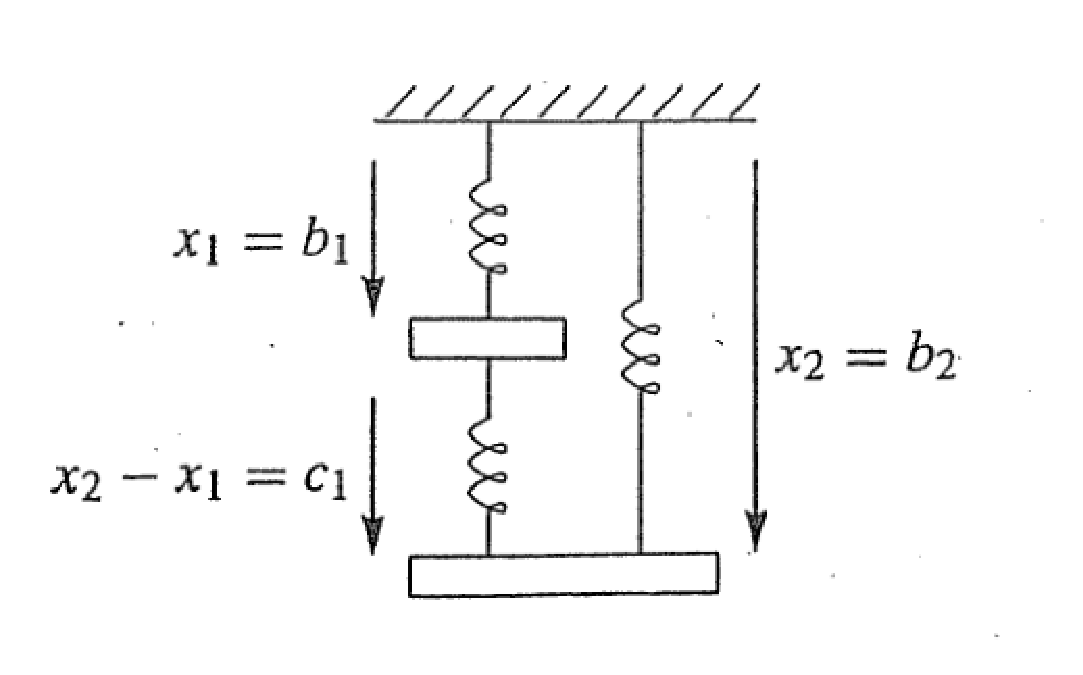
\includegraphics[width=0.7\linewidth]{TeX_files/Part02/chapter04/image/4-4}
		\caption{观测方程和状态方程的质量弹簧当量}
		\label{fig:4-4}
	\end{figure}	
	卡尔曼在每个预测/校正中增加一个弹簧 
	\begin{equation*}
	\hat{x}_{1|1}=b_1  \qquad  \hat{x}_{2|1}=b_1+c_1
	\end{equation*}
	\begin{equation*}
	\hat{x}_2=\hat{x}_{2|2}=\frac{1}{3}(b_1+2b_2+c_1)
	\end{equation*}
	
	解法 \quad  (4.30)中加权最小二乘原则仍给出$\hat{x}_1$和$\hat{x}_2$,最小化为:
	\begin{equation}
	E=\frac{1}{\sigma^2_1}(b_1-x_1)^2+\frac{1}{v^2_1}(c_1+x_1-x_2)^2+\frac{1}{\sigma^2_2}(b_2-x_2)^2
	\end{equation}
	
	加权正常方程$A^TCA=A^TCb$将有$C^{-1}=diag(\sigma^2_1,v^2_1,\sigma^2_2)$,有$C=I,\sigma_1=\sigma_2=V_1=1$:
	\begin{equation}
	\begin{bmatrix}
	\hat{x}_1  \\ \hat{x}_2
	\end{bmatrix}
	=
	\begin{bmatrix}
	b_1-c_1  \\  b_2+c_1
	\end{bmatrix}
	\end{equation}
	给出:
	\begin{equation*}
	\hat{x}_1=\frac{1}{3}(2b_1+b_2-c_1)
	\end{equation*}
	\begin{equation*}
	\hat{x}_2=\frac{1}{3}(b_1+2b_2+c_1)
	\end{equation*}
	
	最新的估计$\hat{x}_2$给了最新的观测值$b_2$一个较大的权重$\frac{2}{3}$。
	
	现在递归计算。关键的一点是$A^TCA$是三对角矩阵(在第8章中,当状态x是一个向量时,它将成为块对角矩阵)。观测方程$A_ix_i=b_i$与状态方程$x_{i+1}=F_ix_i+c_i$相连接,在三对角矩阵$A^TCA$中前向消去法总是一个递归乘法器和一个支点,然后回代是第二个递归,落后于时间。
	
	关键是事实本身,前向递归在观测方程、多达状态方程、还包括时间t=i的基础上,找到最佳估计$\hat{x}_{i|i}$,通常情况下,最终状态的估计$\hat{x}_{n|n}$是我们想要的,然后忘记回代这一步。
	
	回代这一步是调整先前的$\hat{x}_{i|i}$去解释之后的观测方程和状态方程,在时间i之后,以这种方式返回被称为“平滑”,它会使正常方程$A^TCA\hat{x}=A^TCb$产生正确的答案$\hat{x}_{i|n}$。
	
	甚至说寻找$\hat{x}_{i|i}$的前向递归是一个两步法。先前的一步$\hat{x}_{i-1|i-1}$通过时间$i-1$使用所有的信息,接下来状态方程给出一个预测,然后观测值$b_i$加上一个校正,与卡尔曼的滤波一起产生$\hat{x}_{i|i}$,预测和校正为:
	\begin{equation*}
	\hat{x}_{i|i-1}=F_{i-1}\hat{x}_{i-1|i-1}+c_i
	\end{equation*}
	\begin{equation*}
	\hat{x}_{i|i}=\hat{x}_{i|i-1}+K_i(b_i-A_i\hat{x}_{i|i-1})
	\end{equation*}
	该校正像使用增益矩阵$K_i$更新一样被写入,新数据是$c_i$和$b_i$,我们通过最小二乘,一次增加一个方程求解这个完整的系统$Ax=b$。
	
	在递归最小二乘中,有更多的一些东西需要我们计算——估计$\hat{x}_{i|i}$的可信度。协方差矩阵$P_{i|i}=(A^TCA)^{-1}_i$也是递归更新,卡尔曼滤波的每一步都增加一行(或块)到A和C中,一列(或块)到$A^T$和$C$中。预测校正步骤计算$P_{i|i-1}$和$P_{i|i}$,在$\hat{x}_{i|i-1}$和$\hat{x}_{i|i}$中的误差协方差。
	
	公平地说,卡尔曼滤波变得复杂,即使这个计划一直向前。所有的作者试图找到一个清晰的方法去推导$\hat{x}_{i|i}$和$P_{i|i}$的矩阵公式(有多种方式给数值以不同的递归)。平方根滤波用$LDL^T$或$QR$来减少当方差变得很小或很大时的数值不稳定性,我们对卡尔曼滤波的阐述将在第八章进行。
	
	最重要的一点是,协方差矩阵$P_{i|i}$像状态$x_i$具有相同的大小,这个大小与在第i步的观测数量$m_i$无关,如果我们更新最佳拟合直线,我们的矩阵保持2乘以2。
	
	例4.7 \quad (心率)在C=I(单位方差)下,递归找出P和$\hat{x}$:
	
	从$x_1=b_1$开始:\quad\quad  $A_{1|1}=[1]$  给出 $P_{1|1}=(A^TA)^{-1}_{1|1}=[I]$

	加上$x_2-x_1=c_1$:\quad $A_{2|1}=\begin{bmatrix} 1 & 0 \\ -1 & 1 \end{bmatrix}$
	和 $(A^TA)^{-1}_{2|1}=\begin{bmatrix} 1 & 1 \\ 1 & 2 \end{bmatrix}$ 给出  $P_{2|1}=2$
	
	包括$x_2=b_2$:\quad  $A_{2|2}=\begin{bmatrix} -1 & 0 \\ -1 & 1 \\ 0 & 1 \end{bmatrix}$
	和 $(A^TA)^{-1}_{2|2}=\frac{1}{3}\begin{bmatrix} 2 & 1 \\ 1 & 2 \end{bmatrix}$ 给出  $P_{2|2}=\frac{2}{3}$。
	
	第一次估计是$\hat{x}_{1|1}=b_1$(没有平滑!),使用状态方程进行接下来预测$\hat{x}_{2|1}=b_1+c_2$,使用最后的$A_{2|2}$得到校正$\frac{1}{3}(b_1+2b_2+c_1)$。
	
	那些方差$P_{2|1}=2$和$P_{2|2}=\frac{2}{3}$是$(A^TA)^{-1}_{2|1}$和$(A^TA)^{-1}_{2|2}$的最后一项,向量$x_i$引导块的支点$P^{-1}$。这里的2和$\frac{2}{3}$也被看作$b_1+c_1$和$\frac{1}{3}(b_1+2b_2+c_1)$的系数平方和。
	
	回代(平滑)在(4.32)中,调整$\hat{x}_{1|1}=b_1$成为$\hat{x}_1=\frac{1}{3}(2b_1+b_2-c_1)$。
		\section[WGS-84坐标系]{WGS-84坐标系\\World Geodetic System 1984}

		\section[对权重的依赖]{对权重的依赖\\Dependency on the Weights}
一个已经获得最小二乘问题基本知识的人很快提出这个问题:权重有多重要? 如果我们改变他们有点多少,这改变了解决方案? 让我们试着得到一些洞察的问题。 像往常一样,我们从一组观测方程$ A\textbf{\textit{x}}=\textbf{\textit{b}}-\textbf{\textit{e}} $和权重矩阵$C$开始。

我们将观察向量$\textbf{\textit{b}}$分成两个子向量。首先,我们对$\textbf{\textit{b}}_{1}$和$\textbf{\textit{b}}_{2}$的尺寸没有限制。向量$\textbf{\textit{e}}$和矩阵$A$和权重$C$
\begin{align*}
\textbf{\textit{b}}=
\begin{bmatrix}
\textbf{\textit{b}}_{1} \\	
\textbf{\textit{b}}_{2}
\end{bmatrix},
\quad
\textbf{\textit{e}}=
\begin{bmatrix}
\textbf{\textit{e}}_{1} \\	
\textbf{\textit{e}}_{2}
\end{bmatrix},
\quad
A=
\begin{bmatrix}
A_{1} \\	
A_{2}
\end{bmatrix},
\quad
C=
\begin{bmatrix}
C_{1} & 0\\	
0   & C_{2}
\end{bmatrix}.
\end{align*}
这意味着在两组观察之间没有权重耦合。原来的问题变成两个明显的问题:
\begin{align*}
A_{1}\textbf{\textit{x}}&=\textbf{\textit{b}}_{1}-\textbf{\textit{e}}_{1}  &\text{权阵} \ C_{1}                      \\
A_{2}\textbf{\textit{x}}&=\textbf{\textit{b}}_{2}-\textbf{\textit{e}}_{2}  &\text{权阵} \ C_{2}    
\end{align*}
并且我们可以计算每个系统的解。现在有趣的问题是:这些解决方案与整个问题的解决方案相比有什么表现?

我们将看到当我们将第二组的权重$C_{2}$改变为$ C_{2}+\delta C_{2}$时,解$\hat{\textbf{\textit{x}}}$的误差$ \delta \textbf{\textit{x}} $是多少。$ \delta \textbf{\textit{x}} $的表达式涉及一个有用矩阵公式的矩阵计算。原始问题的正规方程是
\begin{align*}
\begin{bmatrix}
A^{T}_{1} &	A^{T}_{2}
\end{bmatrix}
\begin{bmatrix}
C_{1} &	0 \\
0     &	C_{2}
\end{bmatrix}
\begin{bmatrix}
A_{1} \\
A_{2}
\end{bmatrix}  \hat{\textbf{\textit{x}}} = 
\begin{bmatrix}
A^{T}_{1} &	A^{T}_{2}
\end{bmatrix}
\begin{bmatrix}
C_{1} &	0 \\
0     &	C_{2}
\end{bmatrix}
\begin{bmatrix}
\textbf{\textit{b}}_{1} \\
\textbf{\textit{b}}_{2}
\end{bmatrix}.
\end{align*}
这可以写成
\begin{align}
(A^{T}_{1}C_{1}A_{1}+A^{T}_{2}C_{2}A_{2})\hat{\textbf{\textit{x}}}=A^{T}_{1}C_{1}\textbf{\textit{b}}_{1}+A^{T}_{2}C_{2}\textbf{\textit{b}}_{2}.
\end{align}
注意如何收集来自两个问题的正规方程。对正态方程的贡献具有可加性特征。扰动的问题是
\begin{align}
(A^{T}_{1}C_{1}A_{1}+A^{T}_{2}(C_{2}+\delta C_{2} )A_{2})(\hat{\textbf{\textit{x}}}+\delta \textbf{\textit{x}} )=(A^{T}_{1}C_{1}\textbf{\textit{b}}_{1}+A^{T}_{2}(C_{2}+\delta C_{2} )\textbf{\textit{b}}_{2}).
\end{align}
现在从(6.32)中减去(6.31),得到$ \delta \textbf{\textit{x}} $的方程:
\begin{align}
(A^{T}_{1}C_{1}A_{1}+A^{T}_{2}(C_{2}+\delta C_{2} )A_{2})\delta \textbf{\textit{x}} + A^{T}_{2}\delta C_{2}A_{2}\textbf{\textit{x}}=
A^{T}_{2}\delta C_{2}\textbf{\textit{b}}_{2}.
\end{align}
我们令$ N= A^{T}_{1}C_{1}A_{1} + A^{T}_{2}C_{2}A_{2}$和$ \hat{\textbf{\textit{e}}}_{2} = \textbf{\textit{b}}_{2} - A_{2}\textbf{\textit{x}}  $。那么$\hat{\textbf{\textit{x}}}$的变化是
\begin{align}
\delta \textbf{\textit{x}} = ( N + A^{T}_{2}\delta C_{2}A_{2})^{-1}
A^{T}_{2}\delta C_{2} \hat{\textbf{\textit{e}}}_{2}.
\end{align}
下面的重要公式,取自(8.45),得出:
\begin{align}
( N + A^{T}_{2}\delta C_{2}A_{2})^{-1} = N^{-1} - N^{-1}A^{T}_{2}
(A_{2}N^{-1}A^{T}_{2} +(\delta C_{2})^{-1} )^{-1} A_{2} N^{-1}
\end{align}
对于$n$个观测值,该矩阵乘以$ A^{T}_{2}\delta C_{2} \hat{\textbf{\textit{e}}}_{2} $得到$ \delta \textbf{\textit{x}} $。如果我们专注于一个单一的观测值,$ A^{T}_{2} $成为一个$n$乘1矩阵, $ \delta C_{2} $是1乘1.我们命名$ A_{2}N^{-1}A^{T}_{2} = s $并且得到
\begin{align*}
\delta \textbf{\textit{x}} = N^{-1} A^{T}_{2} (1-\dfrac{\delta C_{2}}{1+s\delta C_{2}}s)\delta C_{2}\hat{e}_{2}
\end{align*}
或
\begin{align}
\delta \textbf{\textit{x}} = \dfrac{\hat{e}_{2}\delta C_{2} }{1+s\delta C_{2}}N^{-1}A^{T}_{2}.
\end{align}
表达式(6.36)揭示了几个有趣的事实。解决方案中的变化 $ \delta \textbf{\textit{x}} $(一阶近似)与权重变化$ \delta C_{2} $成正比。在与$A_{2}$中包含的观察相关的未知数中,$ \delta \textbf{\textit{x}} $变化最大。$ N^{-1}A^{T}_{2} $只有来自$N^{-1}$的列的贡献,该列对应于不同于零的$ A^{T}_{2} $。

已经在1823年C.F.高斯找到一个单一权重$ \delta C_{2} $的变化的类似表达式。参见高斯(1995)中的“更新观察变化的未知数”一节。

\begin{figure}[htb]
	\centering
	\includegraphics[width=0.7\linewidth]{TeX_files/Part02/chapter06/image/6-1}
	\caption{Dependence of $ \hat{\textbf{\textit{x}}}$ on $ \delta C_{2}$ \text{在实例} 6.4}
\end{figure}

实例6.4 \ 我们想要演示关于简单最小二乘问题的过程:
\begin{align*}
A = 
\begin{bmatrix}
1&1 \\	
1&2 \\		
-1&1 	
\end{bmatrix} \quad 
\text{和} \quad 
\textbf{\textit{b}}=
\begin{bmatrix}
2 \\	
1 \\		
0 	
\end{bmatrix} \quad 
\text{和} \quad 
C+\delta C_{2} =
\begin{bmatrix}
1   &   & \\	
&   2   & \\		
&   &  1+\delta C_{2} 	
\end{bmatrix} 
\end{align*}
然后$ \delta C_{2} =0 $照常产生解$\hat{\textbf{\textit{x}}}$和残差向量$\hat{\textbf{\textit{e}}}$:
\begin{align*}
\hat{\textbf{\textit{x}}} = \dfrac{1}{3}
\begin{bmatrix}
2 \\	
1 	
\end{bmatrix} \quad 
\text{和} \quad 
\hat{\textbf{\textit{e}}} = \dfrac{1}{3}
\begin{bmatrix}
3 \\	
-1 \\
1	
\end{bmatrix}.
\end{align*}
令$\delta C_{2} =-1 $对应于消除第三观测量。然后$ \hat{\textbf{\textit{x}}}=(3,-1)$是前两行的交点。我们得到第三行元素从(3,-1)到(5/11,5/11)的线段,随着$\delta C_{2} $从-1到$ \infty$。所有权重变化,我们显然可以在三角形内的任何地方获得解。

 $M$文件$dw$反映了发生了什么。
 
 这种权重变化的方法对于少量的观测是极好的。对于一个更大的问题的更多的定性知识,我们转向一个更强大的工具。

现在我们要求更多的定量结果:如果权重改变,投影$\textbf{\textit{p}}=P\textbf{\textit{b}}$在$A$的列空间中移动多少?这种运动的描述是
\begin{align}
tan \alpha = \dfrac{\rVert \textbf{\textit{p}}_{2} - \textbf{\textit{p}}_{1}\rVert c_{1}}{\rVert \textbf{\textit{b}} - \textbf{\textit{p}}_{1}\rVert c_{1}}.
\end{align}
范数由$ \rVert \textbf{\textit{x}} \rVert c_{1}  = \rVert  C_{1}\textbf{\textit{x}} \rVert$加权,$ \alpha$是在行程$ \overline{\textbf{\textit{p}}_{1}\textbf{\textit{p}}_{2}}$处的$\textbf{\textit{b}}$角度。注意图6.2是在$C_{1}$范数中绘制的。在$\textbf{\textit{p}}_{2}$处的角度为$C_{2}$正交;但在$C_{1}$范数中的角度是$ \dfrac{\pi}{2} - \alpha$。从$C_{1}$到$C_{2}$范数的变化导致角度从$ \dfrac{\pi}{2}$改变到$ \dfrac{\pi}{2} - \alpha$。

矩阵$C$的平方根$W$是满足$W^{2}=C$的正定矩阵。这样的矩阵肯定存在,是唯一的,并且非奇异。我们定义$ D = W^{-1}_{1}C_{2}W^{-1}_{1}$,其条件数$c(D)$最大和最小特征值之间的比率可以与角度$ \alpha$相关:
\begin{align}
2\lvert tan\alpha \rvert \leq \sqrt{c(D)} - \dfrac{1}{\sqrt{c(D)}}.
\end{align}

\begin{figure}[!h]
	\centering
	\includegraphics[height=0.23\linewidth]{TeX_files/Part02/chapter06/image/6-2}
	\caption{投影与范数之间的关系. 图是在 $C_{1}$的范数下画的.}
\end{figure}

让我们重复一下:最小二乘问题由系数矩阵$A$,权重$C_{0}$和观测值$\textbf{\textit{b}}$给出。我们考虑所有权重矩阵$C$,使得$ W^{-1}_{0}CW^{-1}_{0}$的特征值位于封闭区间$[s,t]$中。在$C_{0}$的范数中总是找到
\begin{align}
\lvert tan \alpha \rvert \leq \dfrac{1}{2} (\sqrt{\dfrac{t}{s}} - \sqrt{\dfrac{s}{t}}).
\end{align}
角度$ \alpha$测量从$\textbf{\textit{b}}$看到的最小二乘结果的位移。存在至少一个矩阵$C$,其等式符号是有效的。此外,对应于$C_{1}$和$C_{2}$的残差向量的范数之间的比率被限制
\begin{align}
\dfrac{1}{\sqrt{\lambda_{max}}} \leq \dfrac{\rVert \textbf{\textit{b}} - \textbf{\textit{p}}_{1}\rVert c_{1}}{\rVert \textbf{\textit{b}} - \textbf{\textit{p}}_{2}\rVert c_{2}} \leq \sqrt{\lambda_{max}}
\end{align}
其中 $ \lambda_{max}$是该矩阵$ W^{-1}_{2}CW^{-1}_{2}$的最大特征值。

关于最小二乘问题中权重变化的主要结果引自Krarup(1972)。条件数是主要的问题。如果条件数很大,忽略观测值之间可能的相关性的效果可能是危险的。

示例6.5 \ 我们引入具有强相关性的$n$乘$n$的协方差矩阵:
\begin{align*}
\Sigma_{b} =
\begin{bmatrix}
2    &    -1          &        &        & \\
-1   &     2    &    -1        &        & \\
&       \ddots  &  \ddots      & \ddots & \\
&          &         -1    &   2    &  -1 \\
&          &          &       -1    &   2
\end{bmatrix}.
\end{align*}
它的逆具有特殊的形式
\begin{align*}
D = C_{2} = \Sigma^{-1}_{b} =
\left\{
\begin{aligned}
\dfrac{i(n+1-j)}{n+1} \quad \text{for} \ i\leq j\\
\dfrac{j(n+1-i)}{n+1} \quad \text{for} \ i\geq j.
\end{aligned}
\right.
\end{align*}
特征值是$ 4sin^{2} \dfrac{i\pi}{2(n+1)}$,所以条件是$ c(D) \approx \dfrac{4(n+1)^{2}}{\pi^{2}} < n^{2} $。由(6.39)
\begin{align*}
\lvert tan \alpha \rvert \leq \dfrac{1}{2} ( \sqrt{c(D)} - \dfrac{1}{\sqrt{c(D)}}) \approx \dfrac{1}{\pi} (n+1) \rightarrow \infty.
\end{align*}
强相关可以使我们任意地远离对应于$C_{1}=I$的解。

示例6.6 \ 如果$ D = C_{2} = I +t\Sigma^{-1}_{b}$和$ t \approx 10^{-2}$,相关性较弱:
\begin{align*}
c(D) = \dfrac{1+4sin^{2}\dfrac{n\pi}{2(n+1)}}{1+4sin^{2}\dfrac{\pi}{2(n+1)}} \approx 
(1+4t)(1-4t\dfrac{\pi^{2}}{4n^{2}}) \approx 1+4t.
\end{align*}
\begin{align*}
\lvert tan \alpha \rvert \leq \dfrac{1}{2} (\sqrt{1+4t} - \dfrac{1}{\sqrt{1+4t}}) = \dfrac{2t}{\sqrt{1+4t}}.
\end{align*}
另外 $\lvert tan \alpha \rvert < 2t $.
		\section[GPS参考系的意义]{GPS参考系的意义\\Reference Systems Relevant for GPS}
	%%----------------------------第三章结束-------------------------%%	
	
%-----------------------第一部分结束---------------------------%


%-----------------------第二部分开始---------------------------%		
\part[最优估计]{最优估计\\Optimal Estimates}
% \第二篇[目录标题]{正文标题}
	%%----------------------------第四章开始-------------------------%%
	\chapter[随机变量和协方差阵]{随机变量和协方差阵\\Random Variables \\and\\ Covariance Matrices}
	\minitoc %小标题
	\newpage%新页
		\section[最小二乘方程]{最小二乘方程\\The Equations of Least Squares}
本章提出了全球定位的基本数学。在大图片中,我们获得卫星到接收机的伪距测量值。有如此多的卫星,我们希望有更多测量值而不是最少的测量值去确定X,Y,Z,t(位置和时间)。但是这些测量值包含误差(所以我们使用“假,伪”这一词汇去描述观测到的距离)。这就是最小二乘算法:不相容方程组最好的解决方法。

典型的问题是超定线性系统有噪声e(误差):
\begin{equation}\label{eq:4.1}
Ax=b-e
\end{equation}

通常我们有适合n个参数的m个方程(m为观测值)。(未知数$x_1,x_2,...,x_n$可以表示接收机的位置,速度或时间)。方程$Ax=b$无解,因为m>n。我们的任务是找到方程最优解$\hat{x}$(被称为“x帽子”)。

本章建立方程,当噪声向量e是一个随机变量时确定$\hat{x}$。从最简单的假设开始:m的组成部分e独立于标准正态分布(均值为0,方差为1),没有理由相信任何方程在。。。中比其他方程多或少。未加权的最小二乘最小化为$\parallel b-Ax\parallel^2$,即平方差之和,最佳估计$\hat{x}$解答正常方程(标准式方程)
\begin{equation}\label{eq:4.2}
A^TA\hat{x}=A^Tb
\end{equation}	

我们将通过微积分和几何代数得到这些方程,通过通用条件$\partial E/\partial    x_i=0$微积分最小化$E=\|b-Ax\|^2$。通过选择接近于b,组合$A\hat{x}$的A的列数几何最小化E。代数承认$A\hat{x}$是b的投影,在子空间内所有可能组合Ax。

所有理解正常方程$A^TA\hat{x}=A^Tb$的方式值得你的关注,也许这是最重要的线性代数中的应用。解决这些方程数值是一个单独的问题,在大多数情况下,我们只是从系数矩阵$A^TA$(对称正定)入手,然后通过消除不旋转解决。虽然这种方式可以解决,却不是最佳方式:

1、当$A^TA$为病态(系数矩阵A几乎是不独立的列数)时,可能需要更大的数值稳定性,然后有了避免形成$A^TA$的“平方根法”。系数矩阵A相反的列可以提前使其正交化,这在第五章中描述。这个著名的算法使用克-施密特方法,但户主矩阵给出一个更好的方法,奇异值分解可以发挥重要作用。

2、B中的观测值不一定立刻生成,在这种情况下,我们更喜欢递归最小二乘,更新估计的$\hat{x}$来反映最新的观测结果,从一开始就没有重复之前的步骤和验算。

在动态应用(比如移动接收机)中,其状态本身是不断变化的。我们从第i步新的观测中估计不同的的位置向量$x_i$,但这个向量$x_i$与之前的$x_i-1$通过状态方程建立联系,所以每一步是一个两阶段的过程:从状态方程预测(有自己的误差来源),后跟一个修正值去说明下一步新的观测值。

卡尔曼滤波执行这两个步骤。我们在第八章解释这一想法和推导更新公式,在4.3节举出一个例子。
	
3、b中的观测值m可能不是同样地可靠(它们可能不是独立的,误差$e_1,...,e_m$可能是相关的)。$b_i$中的不确定性通过方差$\sigma^2_i$来评估,$e_i$与$e_j$的相关性通过协方差$\sigma_ij$来评估。所有这些数字放入协方差矩阵$\Sigma$中,描述如下:

对称矩阵$\Sigma$告诉我们观测方程$Ax=b$正确的权重,普通最小二乘有隐含的假设,即$\Sigma=\sigma^2I$,独立且平等的方差确定相等的权重,方差越大的方程,可靠性越低,权重越小。

我们将展示逆矩阵$C=\Sigma^-1$为何是加权最小二乘的正确选择。正常方程从$A^TA\hat{x}=A^Tb$变为$A^TCA\hat{x}=A^TCb$,这些方程直接解或者递归解。这一重要的结果不仅是最佳估计$\hat{x}$,而且还是协方差矩阵$P=(A^TCA)^-1$,用来评定最佳估计的可靠性。
	
本章解释概率分布和协方差。正态分布(或高斯分布)中的因素$e^-|x|^2 /2$总是占主导地位,当协方差阵$\Sigma=C^-1$包含在内时系数变为$-x^TCx/2$,这些是基本的想法,定位的应用是这本书的核心。
	
例4.1  最小二乘的一个重要应用是由m个点拟合一条直线。从3个点开始:找到最接近(0,6),(1,0)和(2,0)的线。

\begin{figure}[h]
	\centering
	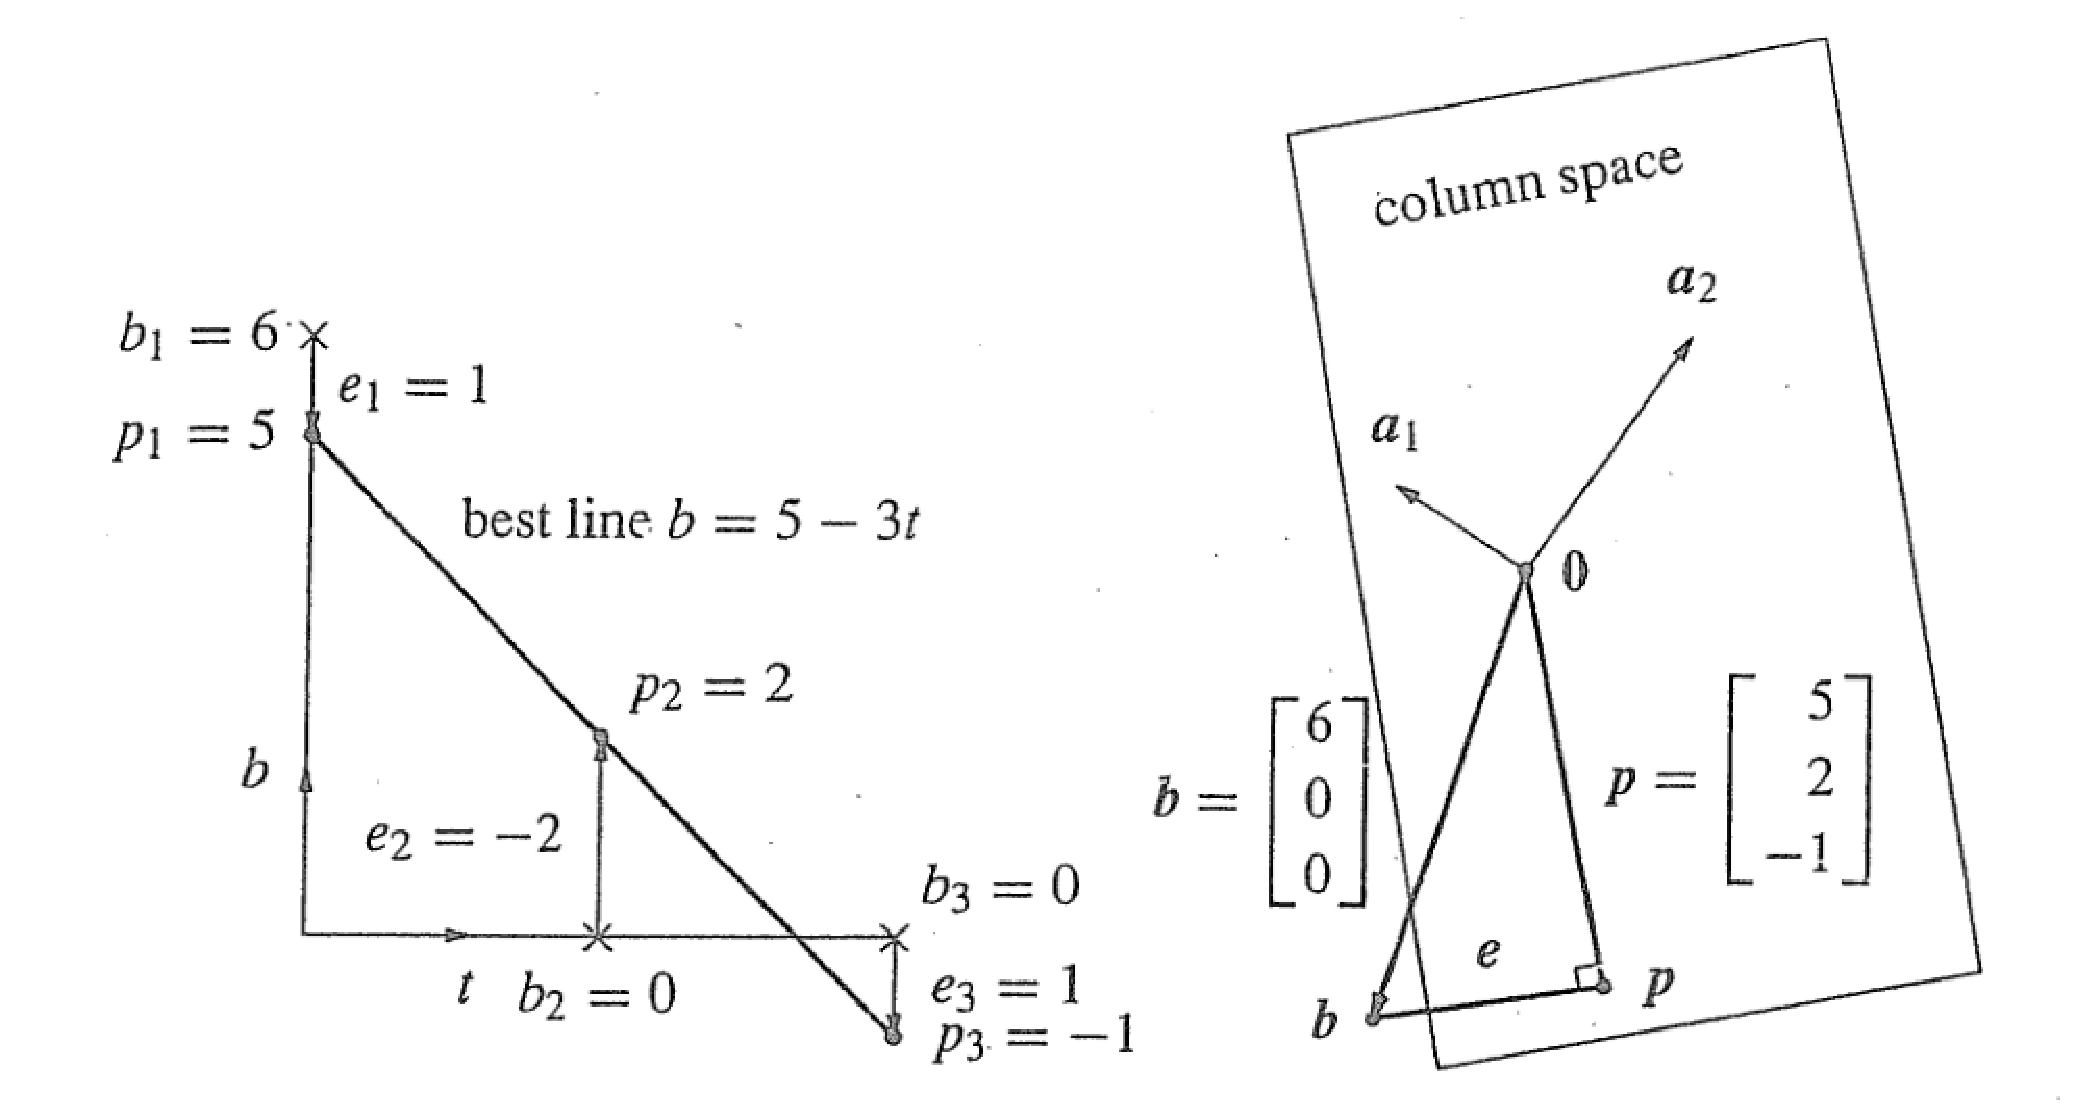
\includegraphics[width=0.7\linewidth]{TeX_files/Part02/chapter04/image/4-1}
	\caption[误差=到直线的垂直距离]{}
	\caption{}
	\label{fig:4-1}
\end{figure}

图4.1\;最好的线和投影:两张图片,同样的问题。这条线有顶点$p=(5,2,-1)$,误差$e=(1,-2,1)$。方程式$A^TA\hat{x}=A^Tb$给出结果$\hat{x}=(5,-3)$,最好的线为$5-3t$,第二张图片中,b的投影为$p=5a_1-3a_2$。

没有直线$b=C+Dt$通过这三个点。我们要求两个数C和D,满足三个方程,这是方程在$t = 0,1,2$匹配给定值$b= 6,0,0$:

	t=0   第一个点在直线$b=C+Dt$  则  $C+D*0=6$ 
	
	t=1   第二个点在直线$b=C+Dt$  则  $C+D*1=0$
	
	t=2   第三个点在直线$b=C+Dt$  则  $C+D*2=0$	
这个3×2的系统没有解决方案:$b =(6,0,0)$不是列(1,1,1)和(0,1,2)的组合。从这些方程中读取A,x和b,解答$A^TA\hat{x}=A^Tb$:

\begin{equation*}
  	A=              
\begin{bmatrix}
    1 & 0 \\ 1 & 1 \\ 1 & 2
\end{bmatrix}
  	\ x=
\begin{bmatrix}
	C \\ D
\end{bmatrix}
  	\ b=
\begin{bmatrix}
	6 \\ 0 \\0
\end{bmatrix}
\end{equation*}
$Ax=b$不可解。

	\subsection[最小化误差]{最小化误差\\Minimizing the Error}
	我们如何使误差$e=b-Ax$尽可能小呢?这是一个有着完美答案的问题。最佳x(被称之为$\hat{x}$)可以通过几何或代数或微积分找到:90°角,或投影向量b,或设置导数平方误差为零。
	
	根据几何学,每一个$Ax$都位于列(1,1,1)和(0,1,2)的平面,在那个平面(图\ref{fig:4-1})内,我们寻找最接近于b的点,最近点则是投影p。
	
	$A\hat{x}$的最佳选择是p,最小的可能错误为$e=b-p$。这三个点的高度$(p_1,p_2,p_3)$确实在一条直线上,因为p是系数C和D两列的组合。在拟合直线中,$\hat{x}$给出了最佳选择$(C,D)$。根据代数将每个向量B分成两部分。列空间中的部分是p,垂直部分在$A^T$零空间的误差为e。我们无法解答方程$(Ax=b)$,但是我们确实可以解答方程$A\hat{x}=p$(通过删除e):
	
	\begin{equation}
	Ax = b = p + e    A\hat{x} = p
	\end{equation}
	前者不可解,后者可解。
	$A\hat{x} = p$解法使得最小可能误差(也就是e),任何x的平方长度为:
	\begin{equation}
 	\|Ax-b\|^2 = \|Ax-p\|^2 + \|e\|^2
	\end{equation}
	
	这是直角三角形定律:$c^2=a^2+b^2$任何在列空间的向量$Ax-p$都垂直于e在$A^T$零空间的误差e,我们通过选择$x=\hat{x}$使$Ax-p$减小到零,让最小的可能误差为$e=(e_1,e_2,e_3)$。
	
	要注意“最小”的含义。$Ax-b$的平方长度最小化:最小二乘解法$\hat{x}$使得$E=\|Ax-b\|^2$尽可能小。
	
	图\ref{fig:4-1}左面板,展示了最接近的线,距离误差为$e_1,e_2,e_3 = 1,-2,1$,这些都是垂直距离,最小二乘线最小化为$E=e^2_1+e^2_2+e^2_3$。
	
	图\ref{fig:4-1}右面板,在三维空间(b,e,p空间)展示了相同的问题,向量b不在A的列空间中。这就是为什么我们无法解决$Ax=b$,没有直线通过这三个点,最小可能误差是垂直向量e,这是$e=b-A\hat{x}$,在三个方程中的误差向量(1,-2,1),与最好直线的距离。这两个数字的后面是基础方程$A^TA\hat{x}=A^Tb$。
	
	注意把误差1,-2,1加上0,误差$e=(e_1,e_2,e_3)$垂直于A的第一列(1,1,1),点乘得$e_1+e_2+e_3=0$。
	
	根据微积分,大多数函数最小化演算。图表最底部和各个方向导数都为零,这里的误差函数E最小平方和$e^2_1+e^2_2+e^2_3=0$(每个方程的误差平方):
	\begin{equation}
	E=\|Ax-b\|^2=(C+D\cdot 0-6)^2+(C+D\cdot 1)^2+(C+D\cdot 2)^2
	\end{equation}
	未知数为C和D,有两个未知数就有两个导数,最小值为零。它们是“偏导数”,因为$\partial E/\partial C$将D看做常数,$\partial E/\partial D$将C看做常数。
	\begin{equation*}
	\partial E/\partial C=2(C+D\cdot 0-6)+2(C+D\cdot 1)+2(C+D\cdot 2)=0
	\partial E/\partial D=2(C+D\cdot 0-6)(0)+2(C+D\cdot 1)(1)+2(C+D\cdot 2)(2)=0
	\end{equation*}
		
	$\partial E/\partial D$包含链式法则的额外因素$(0),(1),(2)$。(从$(C+2D)^2$的最后一个导数是2倍的$C+2D$的2倍),在C导数中对应的因素为1,1,1,因为C总是乘1,1,1,1和0,1,2是A的列并不是偶然的。
	
	现在取消所有项的2倍,收集所有的C和D:
	
	C和D的导数为0:
	\begin{equation}
	3C+3D=6 
	\quad 3C+5D=0 
	\quad A^TA=
	\begin{bmatrix}
	3 & 3 \\ 3 & 5
	\end{bmatrix}
	\end{equation}
	这些方程与$A^TA\hat{x}=A^Tb$是相同的,最好的C和D组成了$\hat{x}$。微积分的方程与线性代数的“正常方程”是相同的,这些是最小二乘的关键方程,当$A^TA\hat{x}=A^Tb$偏导数$\|Ax-b\|^2$为0。
	
	答案为$C=5,D=-3$,因此$b=5-3t$是最好的直线,它与三个点最为接近。当$t=0,1,2$时,这条直线经过$P=5,2,-1$,不能通过$b=6,0,0$,误差为$1,-2,1$,即为向量e。
	
	当x具有微小误差$\Delta x$时,$E=\|b-Ax\|$的一个微积分捷径零导数可以除去E中线性$\Delta x$项,我们可以直接计算线性项:
	\begin{equation*}
	(b-Ax-A\Delta x)^T(b-Ax-A\Delta x)
	\end{equation*}
	包含
	\begin{equation*}
	-\Delta x^TA^T(b-Ax)
	\end{equation*}
	
	相同的项也来自于$(b-Ax)^T(-A\Delta x)$。(记住真正的点产品有$y^Tz=z^Ty$)因此线性部分是这项的两倍,误差$\Delta x$的必须为零:$-\Delta x^TA^T(b-Ax)=0$要求$A^T(b-Ax)=0$。
	
	我们已经恢复在最小化$x=\hat{x}$正常方程$A^TA\hat{x}=A^Tb$。
	
	\subsection[统计与概率的线性代数]{统计与概率的线性代数\\Linear Algebra for Statistics and Probability}
	统计通常处理大量的数据,由于数据往往以矩阵形式存放,我们希望看到$A^TA$,最小二乘$Ax\approx b$是一个线性回归问题,最佳解$hat{x}$适合m个观测值和小于m的n个参数,这是线性代数在统计学中的一个基本应用。
	
	这一章节超越$A^TA\hat{x}=A^Tb$,这些未加权方程假设观测值$b_1,...,b_m$同样可靠,当有好的理由要求在一些观测值中有更高的精度(更小的方差)时,这些方程应该权更重,给予它们多大权重呢?$w_1,...,w_m$?如果观测值$b_i$不独立,协方差矩阵$\Sigma$给出统计误差,下面是关键问题:
	
	1、加权最小二乘和$A^TCA\hat{x}=A^TCb$。
	
	2、方差$\sigma^2_1,...,\sigma^2_m$和协方差矩阵$\Sigma=C^-1$。
	
	\subsection[加权最小二乘]{加权最小二乘\\Weighted Least Squares}
	为了在m个方程$Ax=b$中包含权重,每个方程i乘以权重$w_i$,将这m个权重放入对角矩阵,用$WAx=Wb$代替$Ax=b$,我们希望用最小二乘刚好解决这些方程。
	
	最小二乘方程由$A^TA\hat{x}=A^Tb$变为$(WA)^TWA\hat{x}=(WA)^TWb$。矩阵$C=W^TW$包含$(WA)^TWA$,在最小二乘的中间。
	
	加权最小二乘:
	\begin{equation}
	C=W^TW    A^TCA\hat{x}=A^TCb
	\end{equation}
	当n=1时,A的列数为1,$\hat{x}$从平均数变为加权平均数,最简单的例子:
	\begin{equation}
	\hat{x}=\frac{b_1+...+b_m}{m}
	\end{equation}
	改变为:
	\begin{equation*}
	\hat{x}_W=\frac{w^2_1b_1+...+w^2_mb_m}{w^2_1+...+w^2_m}
	\end{equation*}
	
	平均数$\hat{x}_W$给具有最大权重的观测值$b_i$最大的权重$w_i$,我们总是假设误差为零均值(如果必要的话减去平均数,在测量中并没有片面的偏见)。
	
	我们应该如何选择权重$w_i$?这取决于$b_i$的可靠性,如果观测值方差为$\sigma^2_i$,则$b_i$的均方根误差为$\sigma_i$。当我们以$\sigma_1,...,\sigma_m$分割方程时(左侧和右侧一起),所有的方差等于1。所以权重为$w_i=1/\sigma_i$,$C=W^TW$的对角线包含数字$1/\sigma^2_i$。
	
	统计正确矩阵为:$C=diag(1/\sigma^2_1,...,\sigma^2_m)$。
	
	这仅仅在假设不同方程的误差$e_i$和$e_j$独立时才正确(我们很快定义独立性,方差和协方差)。如果误差是相关的,非对角线元素将在协方差矩阵$\Sigma$中呈现,好的选择仍然是$C=\Sigma^-1$,将在以下章节中描述。

		\section[协方差与最优权]{协方差与最优权\\Covariances and Optimal Weights}

		\section[递归最小二乘(与卡尔曼滤波)]{递归最小二乘(与卡尔曼滤波)\\Recursive Least Squares(and Kalman Filter)}
例4.4 \quad 假设我们已经计算了99个数$b_1,...,b_{99}$的平均数$\hat{x}_{99}$,出现一个新的数$b_{100}$,我们如何在不把前99个数再重新加一遍的情况下得到一个新的平均值$\hat{x}_{100}$(加上$b_{100}$)?我们只想利用$\hat{x}_{99}$和$b_100$。

这是新旧正确的组合$\hat{x}_{100}$,表现为两种形式:

新平均值 
\begin{equation}
\hat{x}_{100}=\frac{99}{100}\hat{x}_{99}+\frac{1}{100}b_{100}=\hat{x}_{99}+\frac{1}{100}(b_{100}-\hat{x}_{99})
\end{equation}
公式中第一项$\frac{99}{100}\hat{x}_{99}$是$(\frac{99}{100})$乘以$(\frac{1}{99})$再乘以$(b_1+b_2+...+b_{99})$,约去99,就是$(\frac{1}{100})$乘以这99个数的和(没有重新加一次!),加上额外的$(\frac{1}{100})$给出所有b的和,再除以100,这就是正确的平均值。

我们更喜欢第二张形式的递推公式(4.24)。通过复杂的创新$b_{100}-\hat{x}_{99}$得到右边更新的$\hat{x}_{99}$,这个创新表明了有多少“新信息”在$b_{100}$中。当$b_{100}$等于旧平均数,创新为0,在这种情况下,更新的$\hat{x}_{100}$就是原来的$\hat{x}_{99}$,校正=预测。

创新是将这个更新公式(4.24)乘以$\frac{1}{100}$,这个增益系数使这个公式正确。想到同样的方法$Ax=b$,从最小二乘解决方程$A_{old}x=b_{old}$入手,新的信息加入,新的观测值$b_{new}$,组合方程$Ax=b$通过最小二乘解出,组合系统为:
\begin{equation}
\begin{bmatrix}
A_{old} \\ A_{new}
\end{bmatrix}
\begin{bmatrix}
x
\end{bmatrix}
\begin{bmatrix}
b_{old} \\ b_{new}
\end{bmatrix}
\end{equation}
引导$\hat{x}_{new}$。

估值$\hat{x}_{new}$从整个系统$Ax=b$得到,在$b_{old}$中的数据仍然有助于$\hat{x}_{new}$,但是我们不想做相同的计算两次。

问题4.1  \quad 我们能否仅用$A_{new}$和$b_{new}$更新$\hat{x}_{old}$和$\hat{x}_{new}$?采取$C=I$
答案 \quad  既然$A^T=\begin{bmatrix} A^T_{old} & A^T_{new}\end{bmatrix}$,我们需要$A^TA$在正常方程:
\begin{equation}
A^TA=A^T_{old}A_{old}+A^T_{new}A_{new}=(known)+(new)
\end{equation}
然后在右边我们需要$A^Tb$,也涉及到新旧值:
\begin{equation}
A^Tb=A^T_{old}b_{old}+A^T_{new}b_{new}=A^T_{old}A_{old}\hat{x}_{old}+A^T_{new}b_{new}
\end{equation}

用$A^TA-A^T_{new}A_{new}$代替$A^T_{old}A_{old}$,然后乘以$(A^TA)^{-1}$找到$\hat{x}_{new}$:
\begin{equation*}
\hat{x}_{new}=(A^TA)^{-1}((A^TA-A^T_{new}A_{new})\hat{x}_{old}+A^T_{new}b_{new})
\end{equation*}

这个更新的公式简化了从原来的值产生新的$\hat{x}$,递推:
\begin{equation}
\hat{x}_{new}=\hat{x}_{old}+(A^TA)^{-1}A^T_{new}(b_{new}-A_{new}\hat{x}_{old})
\end{equation}
最后一项$b_{new}-A_{new}\hat{x}_{old}$是更新,这是我们对于观测值$b_{new}$的预测误差。如果误差为零,数据$b_{new}$与旧估计是完全一致的,没有理由去改变,因此$\hat{x}_{new}=\hat{x}_{old}$。

通常更新项$b_{new}-A_{new}\hat{x}_{old}$不为零,然后(4.28)乘上增益矩阵$K=(A^TA)^{-1}A^T_{new}$找到$\hat{x}$中的变化,增益矩阵是“放大器”,由K(卡尔曼)提出。注意到$A^TA$和$\hat{x}$在更新(4.26)和(4.28)有大小n,比m小。

例4.5 \quad (例4.4完整版)平均值$\hat{u}_{99}=\frac{1}{99}(b_1+...+b_99)$是一元99个方程的最小二乘解,99由1矩阵$A_{old}$是所有的:
\begin{equation*}
\begin{bmatrix}
1 \\ \dots \\ 1
\end{bmatrix}
u=
\begin{bmatrix}
b_1 \\ \dots \\ b_{99}
\end{bmatrix}
A^T_{old}A_{old}\hat{x}_{old}=A^T_{old}b_{old}
\end{equation*}
为:
\begin{equation*}
99\hat{x}_{old}=b_1+...+b_{99}
\end{equation*}
第100个方程是$u=b_{100}=b_{new}$,新的一行是$A_{new}=[1]$,检查所有:

(4.26)更新$A^TA$:
\begin{equation*}
A^TA=99(old)+1(new)=100
\end{equation*}

(4.28)更新$\hat{x}$:
\begin{equation*}
\hat{x}_{100}=\hat{x}_{99}+\frac{1}{100}(b_{new}-A_{new}\hat{x}_{old})=\hat{x}_{99}+\frac{1}{100}(\hat{x}_{100}-\hat{x}_{99})
\end{equation*}

更新的公式与方程(4.24)匹配,增益K是$(A^TA)^{-1}A_{new}=\frac{1}{100}$。

重要的是,你可能认为$A^TA=100$仅仅是对$\hat{x}_{100}$有用的一步,一点也不是,在最小二乘中,$A^TA$(及其逆)是比答案本身更有意义!当我们包含加权矩阵$C=\Sigma^{-1}$时,更新方程(4.26)给出$A^TCA$。我们已经知道为什么想要这个矩阵:逆矩阵$A^TCA=A^T\Sigma^{-1}A$量测$\hat{x}$的可信度P。

在这100个方程的例子中,$b_i$具有相等的可信度,它们有相同的方差$\sigma^2$,来自“标准”正态分布,它们都有$\sigma^2=1$,加权矩阵是$C=I$(正如我们所选),然后$A^TCA=100$的逆量测它们平均值$\hat{x}_{100}$的可信度,如果100个样本有相同的$\sigma^2$,它们的平均值有方差$\sigma^2/100$,当递推最小二乘更新$\hat{x}$时更新矩阵$P=(A^T\Sigma^{-1}A)^{-1}$。

	\subsection[卡尔曼滤波实例]{卡尔曼滤波实例\\Kalman Filter by Example}
	卡尔曼滤波应用在时变最小二乘中,状态x是不断变化的。在离散时间中,我们在每一个$t=i$时间下产生一个估计$\hat{x}_i$,早期的测量仍然给出关于目前状态的信息,因为这种状态是相关的,所以那些$b's$被包含在计算$\hat{x}_i$中。它们可能作用小一些,但是仍然起作用。
	
	例4.6 \quad  有一个未知数x,你的心率,医生第一次测量为$b_1$,之后测量为$b_2$,如果没有理由预测改变,最好的估计$\hat{x}$将是平均数$\frac{1}{2}(b_1+b_2)$,但是如果预测脉率随着年龄的增加而变慢,一个“状态方程”将在这个时间间隔内表示预期变化$c_1$,状态方程为:
	\begin{equation}
	x_2-x_1=c_1+error\epsilon_1
	\end{equation}
	现在我们看关于两个状态值$x_1$和$x_2$。三个方程,它们通过(4.29)联系,观测值和状态方程为:
	\begin{equation}
	x_1 \quad =b_1 
	\end{equation}
	\begin{equation*}
    -x_1+x_2=c_2 
	\end{equation*}
	\begin{equation*}		
	\quad x_2 = b_2
	\end{equation*}
	为:
	\begin{equation*}
	\begin{bmatrix}
	A_{old} \\ A_{state} \\ A_{new}
	\end{bmatrix}
	\begin{bmatrix}
	x_{old}  \\ x_{new}
	\end{bmatrix}
	=
	\begin{bmatrix}
	b_{old} \\ c_{state} \\ b_{new}
	\end{bmatrix}
	\end{equation*}
	重要的是,在这三个方程中都有误差,状态方程并不精确,因为我们的心脏并非以同样的方式变慢,在(4.29)中的状态误差$\epsilon_1$有它自己的方差$\upsilon^2_1$。我们假设误差$e_1,\epsilon_1,e_2$是独立的,这使得一个递归计算(卡尔曼滤波)成为可能。
	
	状态$x_i$通常是一个向量,具有像位置和速度这样的成分(思考追踪一颗空间卫星,或者移动车辆中的GPS),然后(4.29)从旧$x_i$中预测新的位置$x_{i+1}$。通常在$b_i$中会有测量误差的协方差矩阵$\Sigma_i$,在$x_{i+1}=F_ix_i+c_i$中有状态方程误差的协方差$V_i$。		
  
   \begin{figure}
		\centering
		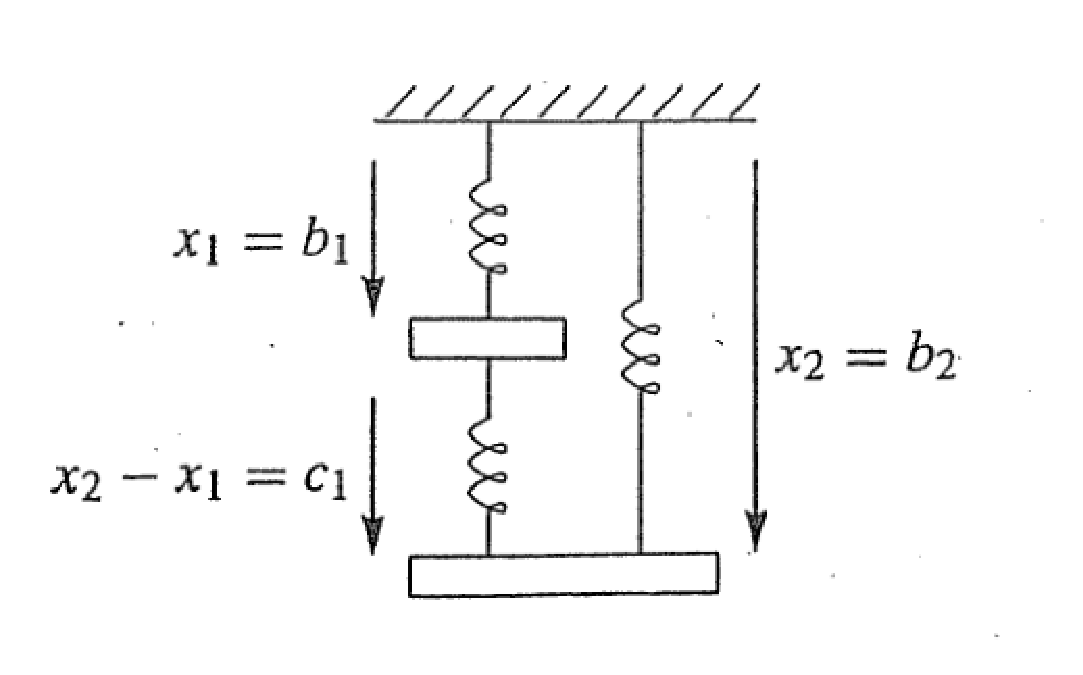
\includegraphics[width=0.7\linewidth]{TeX_files/Part02/chapter04/image/4-4}
		\caption{观测方程和状态方程的质量弹簧当量}
		\label{fig:4-4}
	\end{figure}	
	卡尔曼在每个预测/校正中增加一个弹簧 
	\begin{equation*}
	\hat{x}_{1|1}=b_1  \qquad  \hat{x}_{2|1}=b_1+c_1
	\end{equation*}
	\begin{equation*}
	\hat{x}_2=\hat{x}_{2|2}=\frac{1}{3}(b_1+2b_2+c_1)
	\end{equation*}
	
	解法 \quad  (4.30)中加权最小二乘原则仍给出$\hat{x}_1$和$\hat{x}_2$,最小化为:
	\begin{equation}
	E=\frac{1}{\sigma^2_1}(b_1-x_1)^2+\frac{1}{v^2_1}(c_1+x_1-x_2)^2+\frac{1}{\sigma^2_2}(b_2-x_2)^2
	\end{equation}
	
	加权正常方程$A^TCA=A^TCb$将有$C^{-1}=diag(\sigma^2_1,v^2_1,\sigma^2_2)$,有$C=I,\sigma_1=\sigma_2=V_1=1$:
	\begin{equation}
	\begin{bmatrix}
	\hat{x}_1  \\ \hat{x}_2
	\end{bmatrix}
	=
	\begin{bmatrix}
	b_1-c_1  \\  b_2+c_1
	\end{bmatrix}
	\end{equation}
	给出:
	\begin{equation*}
	\hat{x}_1=\frac{1}{3}(2b_1+b_2-c_1)
	\end{equation*}
	\begin{equation*}
	\hat{x}_2=\frac{1}{3}(b_1+2b_2+c_1)
	\end{equation*}
	
	最新的估计$\hat{x}_2$给了最新的观测值$b_2$一个较大的权重$\frac{2}{3}$。
	
	现在递归计算。关键的一点是$A^TCA$是三对角矩阵(在第8章中,当状态x是一个向量时,它将成为块对角矩阵)。观测方程$A_ix_i=b_i$与状态方程$x_{i+1}=F_ix_i+c_i$相连接,在三对角矩阵$A^TCA$中前向消去法总是一个递归乘法器和一个支点,然后回代是第二个递归,落后于时间。
	
	关键是事实本身,前向递归在观测方程、多达状态方程、还包括时间t=i的基础上,找到最佳估计$\hat{x}_{i|i}$,通常情况下,最终状态的估计$\hat{x}_{n|n}$是我们想要的,然后忘记回代这一步。
	
	回代这一步是调整先前的$\hat{x}_{i|i}$去解释之后的观测方程和状态方程,在时间i之后,以这种方式返回被称为“平滑”,它会使正常方程$A^TCA\hat{x}=A^TCb$产生正确的答案$\hat{x}_{i|n}$。
	
	甚至说寻找$\hat{x}_{i|i}$的前向递归是一个两步法。先前的一步$\hat{x}_{i-1|i-1}$通过时间$i-1$使用所有的信息,接下来状态方程给出一个预测,然后观测值$b_i$加上一个校正,与卡尔曼的滤波一起产生$\hat{x}_{i|i}$,预测和校正为:
	\begin{equation*}
	\hat{x}_{i|i-1}=F_{i-1}\hat{x}_{i-1|i-1}+c_i
	\end{equation*}
	\begin{equation*}
	\hat{x}_{i|i}=\hat{x}_{i|i-1}+K_i(b_i-A_i\hat{x}_{i|i-1})
	\end{equation*}
	该校正像使用增益矩阵$K_i$更新一样被写入,新数据是$c_i$和$b_i$,我们通过最小二乘,一次增加一个方程求解这个完整的系统$Ax=b$。
	
	在递归最小二乘中,有更多的一些东西需要我们计算——估计$\hat{x}_{i|i}$的可信度。协方差矩阵$P_{i|i}=(A^TCA)^{-1}_i$也是递归更新,卡尔曼滤波的每一步都增加一行(或块)到A和C中,一列(或块)到$A^T$和$C$中。预测校正步骤计算$P_{i|i-1}$和$P_{i|i}$,在$\hat{x}_{i|i-1}$和$\hat{x}_{i|i}$中的误差协方差。
	
	公平地说,卡尔曼滤波变得复杂,即使这个计划一直向前。所有的作者试图找到一个清晰的方法去推导$\hat{x}_{i|i}$和$P_{i|i}$的矩阵公式(有多种方式给数值以不同的递归)。平方根滤波用$LDL^T$或$QR$来减少当方差变得很小或很大时的数值不稳定性,我们对卡尔曼滤波的阐述将在第八章进行。
	
	最重要的一点是,协方差矩阵$P_{i|i}$像状态$x_i$具有相同的大小,这个大小与在第i步的观测数量$m_i$无关,如果我们更新最佳拟合直线,我们的矩阵保持2乘以2。
	
	例4.7 \quad (心率)在C=I(单位方差)下,递归找出P和$\hat{x}$:
	
	从$x_1=b_1$开始:\quad\quad  $A_{1|1}=[1]$  给出 $P_{1|1}=(A^TA)^{-1}_{1|1}=[I]$

	加上$x_2-x_1=c_1$:\quad $A_{2|1}=\begin{bmatrix} 1 & 0 \\ -1 & 1 \end{bmatrix}$
	和 $(A^TA)^{-1}_{2|1}=\begin{bmatrix} 1 & 1 \\ 1 & 2 \end{bmatrix}$ 给出  $P_{2|1}=2$
	
	包括$x_2=b_2$:\quad  $A_{2|2}=\begin{bmatrix} -1 & 0 \\ -1 & 1 \\ 0 & 1 \end{bmatrix}$
	和 $(A^TA)^{-1}_{2|2}=\frac{1}{3}\begin{bmatrix} 2 & 1 \\ 1 & 2 \end{bmatrix}$ 给出  $P_{2|2}=\frac{2}{3}$。
	
	第一次估计是$\hat{x}_{1|1}=b_1$(没有平滑!),使用状态方程进行接下来预测$\hat{x}_{2|1}=b_1+c_2$,使用最后的$A_{2|2}$得到校正$\frac{1}{3}(b_1+2b_2+c_1)$。
	
	那些方差$P_{2|1}=2$和$P_{2|2}=\frac{2}{3}$是$(A^TA)^{-1}_{2|1}$和$(A^TA)^{-1}_{2|2}$的最后一项,向量$x_i$引导块的支点$P^{-1}$。这里的2和$\frac{2}{3}$也被看作$b_1+c_1$和$\frac{1}{3}(b_1+2b_2+c_1)$的系数平方和。
	
	回代(平滑)在(4.32)中,调整$\hat{x}_{1|1}=b_1$成为$\hat{x}_1=\frac{1}{3}(2b_1+b_2-c_1)$。
		\section[正态分布与$\chi^{2}$]{正态分布与$\chi^{2}$\\The Normal Distribution and $\chi^{2}$}

		\section[均值、方差与协方差]{均值、方差与协方差\\Mean,Variance,and Covariance}

		\section[均值与协方差的传播律]{均值与协方差的传播率\\Propagation of Means and Covariances}

		\section[单位权方差估计]{单位权方差估计\\Estimating the Variance of Unit Weight}

		\section[数值计算方法与最小二乘]{数值计算方法与最小二乘\\Numerical Methods for Weighted Least Squares}

		\section[置信椭圆]{置信椭圆\\Confidence Ellipses}

		\section[质量控制]{质量控制\\Quality Control}

	%%----------------------------第四章结束-------------------------%%

	%%----------------------------第五章开始-------------------------%%
	\chapter[随机过程]{随机过程\\Random Processes}
	\minitoc %小标题
	\newpage%新页
		\section[连续时间中的随机过程]{连续时间中的随机过程\\Random Processes in Continuous Time}

		\section[离散时间中的随机过程]{离散时间中的随机过程\\Random Processes in Discrete Time}
	第四章从连续随机变量开始,本章我们用类似的方法进行。(这儿有一段看不清)
	
		\[ x_{k}=F_{k-1}x_{k-1}+G_{k}\varepsilon_{k} \]
		\begin{equation}\label{5.24}
	b_{k}=A_{k}x_{k}+e_{k}
	\end{equation}
	
	
	假设状态方程中的不相关过程噪声 $ \varepsilon_{k} $ 有协方差矩阵 $\sum_{\varepsilon,k} $ 。假设观测噪声  $ e_{k} $ 是不相关的并且具有零均值,通过协方差传播率,我们得到关于协方差 $ x_{k} $ 的以下递归方程:
	
	\begin{equation}\label{5.25}
	\sum\nolimits_{k}=F_{k-1}\sum\nolimits_{k-1}F_{k-1}^{T}+G_{k}\sum\nolimits_{\varepsilon,k}G_{k}^{T}
	\end{equation}
		然而,模型(5.24)允许随机过程噪声 $ \varepsilon_{k} $ 的时间相关。这种相关常常发生在实践的模型中。它可以通过增加状态向量 $ x_{k} $  来正确处理。假设 $ \varepsilon_{k} $ 可以分为相关量 $ \varepsilon_{1,k} $ 和不相关量 $ \varepsilon_{2,k}: \varepsilon_{k} = \varepsilon_{1,k} + \varepsilon_{2,k} $,我们假设$\varepsilon_{1,k} $可以模型化为差分方程
		
			\[ \varepsilon_{1,k}=G_{\varepsilon,\varepsilon_{1,k}}+\varepsilon_{3,k-1} \]
			
		 $ \varepsilon_{3} $	是不相关噪声的向量,增强状态向量 $ x_{k}^{'} $ 通过以下式子给出
		 
		 \[ x_{k}^{'}=\begin{bmatrix} x_{k}  \\ \varepsilon_{1,k}\end{bmatrix} \quad \]
		 
		 增强状态方程仅由不相关干扰给出
		 
		 	\begin{equation}\label{5.26}
		 x_{k}^{'}=\begin{bmatrix} x_{k}  \\ \varepsilon_{1,k}\end{bmatrix} \quad=\begin{bmatrix} F&G  \\ 0&G_{\varepsilon}\end{bmatrix} \quad \begin{bmatrix} x_{k-1}  \\ \varepsilon_{1,k-1}\end{bmatrix} \quad
		 + \begin{bmatrix} G&0 \\ 0&I\end{bmatrix} \quad \begin{bmatrix} \varepsilon_{2,k-1}  \\ \varepsilon_{3,k-1}\end{bmatrix} 
		 \end{equation}
		 接下来我们考虑系统扰动的四个特定模型。在每种情况下以标量描述。
		 
		 \textbf{实例5.7}(随机常数)随机常数是有固定随机振幅的非动态量,该过程由以下方程描述
		 
		 \[ x_{k}=x_{k-1} \]
		 
		 随机常数可能有随机初始状态 $ x_{0} $。
		 
		 \textbf{实例5.8}(随机游走)该过程由以下方程描述
		 
		 	\[ x_{k}=x_{k-1}+\varepsilon_{k} \]
		 
		 噪声的方差为
		 
		 \[ E\left\lbrace \varepsilon_{k}^{2}\right\rbrace = E\left\lbrace(x_{k}-x_{k-1})^{2} \right\rbrace =E\left\lbrace x_{k}^{2} \right\rbrace +E\left\lbrace x_{k-1}^{2} \right\rbrace -2E\left\lbrace x_{k}x_{k-1} \right\rbrace =2\sigma_{x}^{2} \]
		 
		 \textbf{实例5.9}(随机斜坡)随机斜坡是随时间线性增长的过程,随机斜坡的增长率是具有给定方差的随机量。我们需要两个状态元素来描述随机斜坡:
		 
		 	\[ x_{1,k}=x_{1,k-1}+(t_{k}-t_{k-1})x_{2,k-1}+\varepsilon_{1,k-1} \]
		 \[ x_{2,k}=x_{2,k-1}+\varepsilon_{2,k} \]
		 
		 \textbf{实例5.10}(指数相关随机变量)
		 
		 \[ x_{k}=e^{-\alpha(t_{k}-t{k-1})}x_{k-1}+\varepsilon_{k}\]
		 
		 我们有$ \varepsilon_{k}=x_{k}-e^{-\alpha(t_{k}-t_{k-1})} $ 。时间差是 $ \Delta t=t_{k}-t_{k-1} $。根据(5.20)我们有$ E\left\lbrace \varepsilon_{k}^{2}\right\rbrace =\sigma^{2}(1-e^{-2 \alpha   \bigtriangleup t  })  $.
		 
		 实例5.7-5.10是许多线性滤波器的基础,接下来我们讨论三个和GP应用相关的例子,见 Axelrad and Brown (1996)
		 
		 \textbf{实例5.11}(离散随机斜坡)通常随机误差表现出确定的时间增长行为。离散随机斜坡是一个随时间线性增长的函数,通常可以用来描述随机误差,随机斜坡的增长率是具有给定方差的随机量。这个模型的很好的例子是偏移 $  b $ 的行为和接收机钟的漂移 $ d $ 。
		 
		 需要两个状态分量来描述随机斜坡,所以我们用向量 $ x_{k} $ 和矩阵方程:
		 
		 
		 	\begin{equation}\label{5.27}
		 x_{k}=Fx_{k-1}+\varepsilon _{k} \quad with \quad  x_{k}= \begin{bmatrix} b_{k}  \\ d_{k}\end{bmatrix} \quad and\quad F=\begin{bmatrix} 1&\Delta t  \\ 0 & 1 \end{bmatrix}
		 \end{equation}
		  
		 
		 偏移 $ b $ 是随机斜坡过程。漂移 $ d  $ 描述了斜坡的斜率。$ F $ 的第二行给了从 $ d_{k-1} $ 到 $ d_{k} $ 的斜率的变化。第一行给了随机游走:
		 
		 \[ b_{k}=b_{k-1}+\Delta t d_{k-1}+random error \]
		 
		 
		 接下来,我们估计观测误差 $ \sum = E\left\lbrace \varepsilon \varepsilon^{T} \right\rbrace  $  的协方差矩阵。我们从一个连续的系统公式开始,
		 
		 并整合一个时间步骤:
		 
		  \[ \epsilon_{k}=\int_{t_{k-1}}^{t_{k}}F(t_{k},\tau)\epsilon(\tau)d\tau \]	
		  
		  这产生
		  
		 	\begin{equation*}
		 \begin{aligned}
		 E\left\lbrace \epsilon_{k} \epsilon_{k}^{T} \right\rbrace &=E\left\lbrace\int_{t_{k-1}}^{t_{k}}\int_{t_{k-1}}^{t_{k}} F(t_{k},\tau)\epsilon(\tau)\epsilon(\sigma)^{T}F(t_{k},\sigma)d\tau d\sigma \right\rbrace \\
		 &= \int_{t_{k-1}}^{t_{k}} F(t_{k},\tau)\sum(\tau)F(t_{k},\tau)^{T}d\tau
		 \end{aligned}
		 \end{equation*}
		 
		  矩阵 $\sum (\tau)$ 是一个谱密度矩阵。让偏移和漂移的频谱幅度为  $ s_{b} $ 和 $ s_{d}$ :
		  
		  	\[ \sum = \begin{bmatrix} s_{b}&0  \\ 0&s_{d} \end{bmatrix} \quad \]
		  	
		  然后被积函数是一个2*2的矩阵
		  
		  \[ F\sum F_{T} = \begin{bmatrix} s_{b}+s_{d} \tau ^{2} & s_{d}\tau \\s_{d}\tau & s_{d} \end{bmatrix} \quad  \]
		  
		  然后我们得到了协方差矩阵的公式:
		  
		  	\begin{equation}\label{5.28}
		  \begin{aligned}
		  E\left\lbrace\epsilon \epsilon^{T} \right\rbrace &=\int_{t_{k-1}}^{t_{k}} \begin{bmatrix}
		  s_{b}+s_{d}\tau^{2}&s_{d}\tau\\s_{d}\tau&s_{d}
		  \end{bmatrix}\quad d\tau\\
		  &=\begin{bmatrix}
		  s_{b}\Delta t+s_{d}(\Delta t)^{3}/3&s_{d}(\Delta t)^{2}/2\\s_{d}(\Delta)^{2}/2&s_{d}\Delta t
		  \end{bmatrix}
		  \end{aligned}
		  \end{equation}
		  
		  白噪声的频谱幅度$ s_{b} $和接收机钟差 $ s_{d} $ 的典型值为  $ 4\times10^{-19} $ 和 $ 15\times10^{-19} $ 。
		  一个典型的时间步长是  $ \Delta t=20s $ 。在这种情况下协方差矩阵 $ \sum\nolimits_{clock} $ 是:
		  
		  	\[ \sum\nolimits_{clock}=E\left\lbrace \epsilon \epsilon^{T} \right\rbrace =\begin{bmatrix}
		  400004&300\\300&3000
		  \end{bmatrix}\times10^{-19} \] 
		  
		  \textbf{实例5.12}一个GPS接收机的过程模型包括与接收机钟偏和钟漂相组合的接收机的三个坐标。动态过程仍由(5.27)给出,状态向量X有五个分量:
		  
		  	\[ x_{k}=\begin{bmatrix}
		  x\\y\\z\\b\\d
		  \end{bmatrix}\quad and \quad  F=\begin{bmatrix}
		  1&0&0&0&0\\0&1&0&0&0\\0&0&1&0&0\\0&0&0&1&\Delta t\\0&0&0&0&1
		  \end{bmatrix}  \]
		  
		  静态接收机的协方差矩阵是:
		  
		 	\begin{equation}\label{5.29}
		 \sum\nolimits_{static} = E\left\lbrace \epsilon \epsilon^{T} \right\rbrace = \begin{bmatrix}
		 \sum\nolimits_{position}&0\\0&\sum\nolimits_{clock}
		 \end{bmatrix}
		 \end{equation}
		  
		  
		  矩阵 $ \sum\nolimits_{clock} $ 反应了接收机钟的随机分布。协方差矩阵 $ \sum\nolimits_{position} $ 反映了和测站相关的模型噪声。当接收机放在固定的位置(静态接收机)很自然的设为 $ \sum\nolimits_{position}=0$。然而这意味着所有新的测站信息将被忽略并且没有意义。所以我们人为的让测站有一个小的偏差以便滤波不会卡住。
		  
		  \textbf{实例5.13}运动接收器是一个可以四处移动的GPS接收器,他通常放在低速移动并且不会突然变速的车上。现在状态向量包含八个分量:
		  三个坐标,三个速度,和两个时钟项:
		  
		  	
		  \[ x_{k}=\begin{bmatrix}
		  x\\y\\z\\\dot{x}\\\dot{y}\\\dot{z}\\b\\d
		  \end{bmatrix}\quad 和 \quad  F=\begin{bmatrix}
		  1&0&0&\Delta t&0&0&0&0\\0&1&0&0&\Delta t&0&0&0\\0&0&1&0&0&\Delta t&0&0\\0&0&0&1&0&0&0&0\\0&0&0&0&1&0&0&0\\0&0&0&0&0&1&0&0\\0&0&0&0&0&0&1&\Delta t\\0&0&0&0&0&0&0&1
		  \end{bmatrix}  \]
		  
		  协方差为
		  
		 \begin{equation}\label{5.30}
		 \sum\nolimits_{kinematic}=E\left\lbrace \epsilon\epsilon^{T}   \right\rbrace=\begin{bmatrix}
		 \sum\nolimits_{position}&\sum\nolimits_{position,velocity}&0\\\sum\nolimits_{position,velocity}&\sum\nolimits_{velocity}&0\\0&0&\sum\nolimits_{clock}
		 \end{bmatrix} 
		 \end{equation}
		  
		  矩阵 $ \sum\nolimits_{velocity} $ 通常对水平分量和垂直分量使用不同的值,汽车基本不改变它的垂直速度,但它可以快速加速或减速。当然,如果  $ \sum\nolimits_{kinematic} $ 中的对角项的方差很大,如下一张描述的滤波过程,将不会对位置的精度有明显提高。
		  
		  
		 \textbf{ 实例5.14}(高斯-马尔克夫过程)令 $ x_{k} $ 为具有零均值并且自相关指数递减的静态随机过程:
		 
		 \[ R_{x}(t_{2}-t_{1})=\sigma^{2}e^{-\alpha|t_{2}-t_{1}|} \] 
		 
		 
		 当输入  $v\varepsilon_{k} $ 是具有等于1的功率谱密度的零平均白噪声时,这种类型的随机过程可以被建模为线性系统的输出。 (在标准时间序列文献中,这被称为AR(1)模型.AR(1)表示阶数1的自回归)。这种类型的过程的差分方程模型是:
		  \[  x_{k}=Fx_{k-1}+G\epsilon_{k}\]
		 \begin{equation}\label{5.31}
		b_{k}=x_{k}
		\end{equation}
		 
		 为了使用这个模型,我们需要求解未知标量参数 $ F $ 和 $ G $ 作为参数  $ \alpha $ 的函数。 为此,我们在两边乘以(5.31)两边并取
		\[ \textbf{Table 5.2} System models of discrete-time random processes  \]
		\[ \begin{tabular}{lcr}
		\hline
		$ Process\quad type $ & $ Autocorrelation\quad R_{x}(\tau) $ & $State\quad model $ \\
		\cline{1-3}
		$ Random \quad constant $ & $  R_{x}(\Delta t)=\sigma^{2}$ & $  x_{k}=x_{k-1},\sigma^{2}{x_{0}}=\sigma^{2}$\\
		$ Random \quad walk $&$  R_{x}(\Delta t)= \infty  $&$  x_{k}=x_{k-1}+\epsilon_{k},\sigma^{2}{x_{0}}=0$\\
		
		$ Random \quad ramp $ &$ \quad$&$  x_{1,k}=x_{1,k-1}+\Delta t x_{2,k-1}$\\
		
		$  \quad  $ &$ \quad$&$  x_{2,k}=x_{2,k-1} $\\
		
		$  Exponenitially  $  & $ R_{x}(\Delta t)=\sigma^{2}e^{-\alpha|\Delta t_{k}|} $ & $ x_{k}=e^{-\alpha|\Delta t|}x_{k-1}\epsilon_{k}$\\
		
		$ correlated$ & $  \quad   $ & $ \sigma^{2}{x_{0}}=\sigma^{2},\Delta t = t_{k}-t_{k-1} $ \\
		
		\hline
		\end{tabular} \]      
		 期望值以获得方程
		 
		 \[ E\left\lbrace x_{k}x_{k-1} \right\rbrace =FE\left\lbrace x_{k-1}x_{k-1}\right\rbrace +GE\left\lbrace \epsilon_{k}x_{k-1}\right\rbrace \]
		 
		 \begin{equation}\label{5.32}
		 \sigma^{2}e^{-\alpha}=F\sigma^{2}
		 \end{equation}
		 
		 假设 $ \varepsilon_{k} $ 是不相关的并且 $ E\left\lbrace \varepsilon_{k}\right\rbrace =0 $,则 $ E\left\lbrace \varepsilon_{k}\varepsilon_{k} \right\rbrace = 0 $。转换矩阵是 $ F=e^{-\alpha} $。接下来是由(5.31)定义的状态变量并取其期望值:
		 
		 \[ E\left\lbrace x_{k}^{2}\right\rbrace = F^{2}E\left\lbrace x_{k-1}x_{k-1}\right\rbrace+G^{2}E\left\lbrace \epsilon_{k}\epsilon{k}\right\rbrace \]
		 
		\begin{equation}\label{5.33}
		\sigma^{2}=\sigma^{2}F^{2}+G^{2}
		\end{equation}
		 
		  因为系统方差是  $ E\left\lbrace\varepsilon_{k}^{2}\right\rbrace=1 $ 。我们 将$ F=e^{-\alpha} $ 插入到5.33得到 $ G=\sigma\sqrt{1-e^{-2\alpha}}   $ 。完整的模型是
		  	
		  \[ x_{k}=e^{-\alpha}x_{k-1}+\sigma\sqrt{1-e^{-2\alpha}}\epsilon_{k} \]
		 
		 \[ b_{k}=x_{k} \]
		 
		 其中, $ E\left\lbrace \varepsilon_{k}\right\rbrace=0  $ , $E\left\lbrace \varepsilon_{k}\varepsilon_{j}\right\rbrace=\delta_{jk}$。
		 
		 理想情况下,随机过程应基于管理系统错误噪声的物理规律。 确切的表述通常是不可能的,因为底层物理学不是很好理解,或者因为实现理想的随机过程将产生麻烦的解决方案。 高斯马尔可夫模型(相关指数衰减)非常有用,只需要一个参数 $ \alpha $。
		\section[模型]{模型\\Modeling}

在应用工程中,很少发生给定的物理问题是确切的形式:


\[ x_{k}=F_{k-1}x_{k-1}+\epsilon_{k} \]

\[ b_{k}=A_{k}x_{k}+e_{k} \]

\begin{figure}[h]
	\centering
	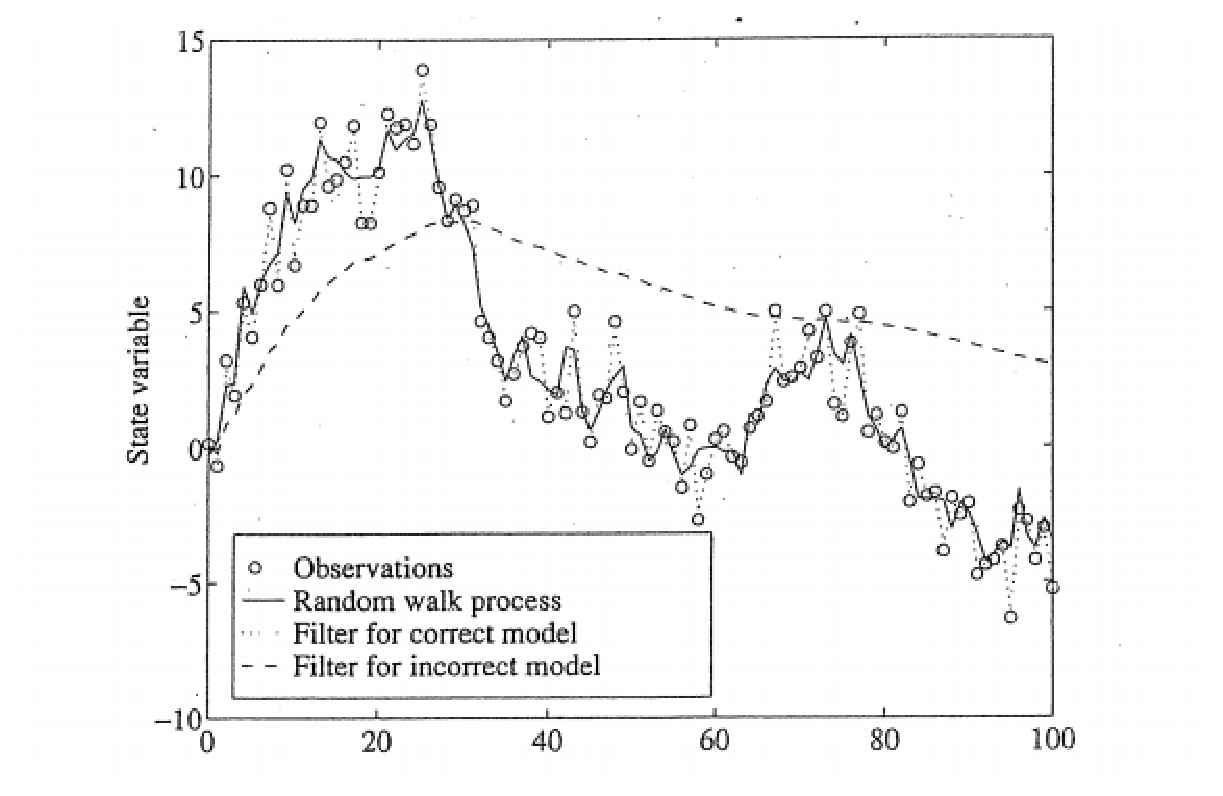
\includegraphics[width=0.7\linewidth]{TeX_files/Part02/chapter05/image/3}
	\caption{Correctly and incorrectly filtered random walk process}
\end{figure}

最常见的是,原始问题必须被修改以适应适当的形式。 这种扭曲通常被称为建模,它在卡尔曼滤波应用中是非常重要的。 良好的建模导致良好的效果; 糟糕的造型导致糟糕的结果。 它是如此简单。 建模过程没有设定规则,它通常需要一些想象力。也许最好变得擅长建模的方法是看各种各样的例子。 我们从Brown and Hwang(1997)的一个例子开始,展示了误差模型的影响。

\textbf{示例5.15}考虑一个实际上是随机游走但是被错误地建模为随机常数 $ c $ 的过程。 然后我们有真正的模型

\[ x_{k}=x_{k-1}+\epsilon_{k}, \quad \epsilon_{k}=单位高斯白噪声,\sigma^{2}{x_{0}}=1 \]

\[ b_{k}=x_{k}+e_{k},\quad k=0,1,2,...\sigma^{2}\left\lbrace e_{k}\right\rbrace =0,1\]

和不正确的模型

\[ x_{k}=c,\quad c~N(0,1) \]
\[ b_{k}=x_{k}+e_{k},\quad k=0,1,2,...\sigma^{2}\left\lbrace e_{k}\right\rbrace=0,1 \]

错误的模型有 $ F_{k}=1,\sum\nolimits_{\varepsilon,k}=0,\sum\nolimits_{e,k}=0.1, \hat{x_{0}}=0 $ 和 $ P_{0}^{-1}=1 $。正确的模型参数是一样的,除了 $ \sum\nolimits_{\varepsilon,k}=1 $,而不是0.

图5.3中显示了100秒的处理结果。还使用另一组N(0,1)个随机数生成该样本处理的测量序列 $ b_{k} $。首先使用不正确的模型处理该测量序列,再次使用正确的模型进行处理。结果与图5.3中的样品过程一起显示。在这种情况下,测量噪声相对较小()$ \sigma\approx 0.3 $,我们注意到,在最初的几个步骤之后,建模过滤器的估计很差。这是由于过滤器的增益随着每个后续步骤而减小。在第100步,增益比起初要低两个数量级。因此,过滤器变得非常缓慢,不会随机游走。如果模拟被允许进一步,那将会变得更加缓慢。


实例5.15就是这样。假设过程或过程的任何方面永远永远永远是永恒的,任何模型都是一个风险模型。在物理世界中,极少数事物绝对不变。这种类型的分歧问题的明显补救办法总是将一些过程噪声插入到每个状态变量中。即使有一定程度的不合适的风险,也可以做到这一点;它造就了比其他方式更安全的过滤器。它也有助于彻底解决潜在的问题。通常,随机游走模型是时间跨度较大的更安全的模型,通常优于超过真正恒定模型的模型。

选择合适的流程模型始终是一个重要的考虑因素。需要一定量的常识判断来决定适合手头情况的模式,但同时不会太复杂。
例如,没有过程会随机游走到无限远。某些地方受到某种限制:对流层短时间内看起来像随机游走。但是假设整天没有测量?我们对对流层方法的了解不足吗?不,当然不。我们知道对流层天顶延迟可以预测为2.4米,约2%的不确定性或更好。

\subsection{计算自相关}

以一个恒定的时间间隔计算一个有序数据集 $ a_{0},a_{1}.1_{2},...a_{n-1} $ 的自相关性是很简单的。 首先我们计算平均值m(平均值)。 第二,我们可以想象数据排列成两行:

\[ shift = 0:\begin{bmatrix}
a_{0}&a_{1}&a_{2}&a_{3}&a_{4}&...\\ a_{0}&a_{1}&a_{2}&a_{3}&a_{4}&...
\end{bmatrix}\quad auto(0)=\sum_{0}^{n-1}a_{i}a_{i}/n \] 


我们将元素  $ a_{i}a_{i} $  相互重叠,并添加。 现在下移一行:

 \[ shift = 1:\begin{bmatrix}
a_{0}&a_{1}&a_{2}&a_{3}&a_{4}&...&\quad\\ \quad&a_{0}&a_{1}&a_{2}&a_{3}&a_{4}&...
\end{bmatrix}\quad auto(0)=\sum_{1}^{n-1}a_{i}a_{i-1}/n \] 

再次,我们将元素相互叠加。 这一次,术语数减少了一个。 我们继续移动,每次我们将总和除以数据数n。 M文件具有以下核心代码:

\[ auto=autocoor(a) \]
\[ m=mean(a) \]
\begin{figure}[h]
	\centering
	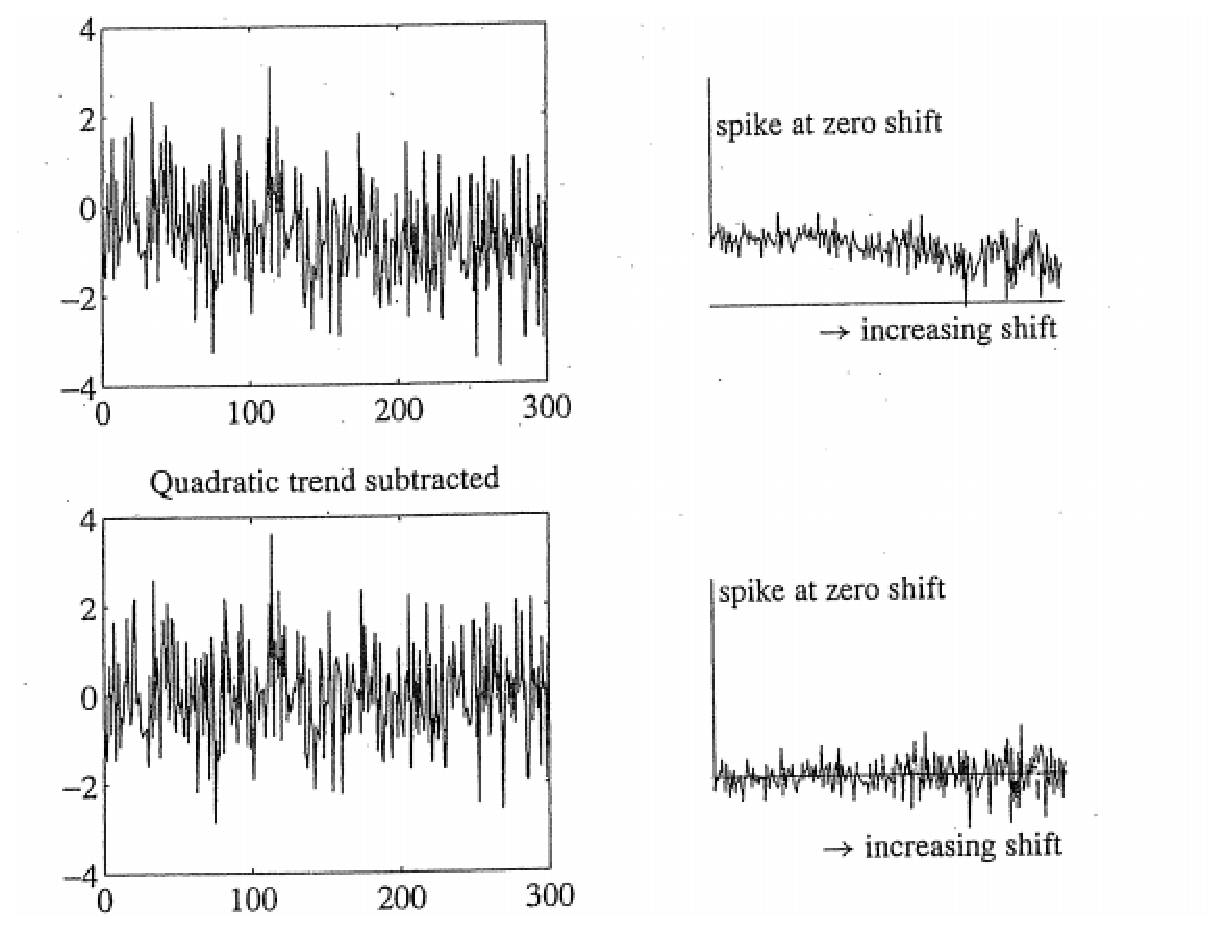
\includegraphics[width=0.7\linewidth]{TeX_files/Part02/chapter05/image/4}
	\caption{Autocorrelation for random data. The peak at zero measures the variance.}
	\label{ }
\end{figure}

 \[ for \quad shift = 0:n-2 \]
\[ q=0 ;\]
\[ for\quad t=1:n-shift \]
\[ q=q+(a(t)-m)*(a(t+shift)-m); \]
\[ end \]
\[ auto(shift+1)=q/n ;\]
\[ end \]


图5.4随机数据的自相关图。 零点的峰值测量方差。

大量转移的总量只包含少量的术语; 重叠数 $ n-shift-1 $ 很小。 统计做法是省略转移产品总额的20%(或类似分数); 他们不那么可靠。 幸运的是,我们对小转换的自相关最感兴趣,因为它们揭示了数据的性质。 所以自动化的结果对于小转换最重要,见图5.4。

我们把总和除以 $  n $,而不是  $ n-shift-1 $ 。这正好确保了

 \begin{equation}\label{5.34}
R=\begin{bmatrix}
auto(0)&auto(1)&...&auto(n-1)\\auto(1)&auto(0)&...&auto(n-2)\\ \colon&\colon&\ddots&\colon\\auto(n-1)&auto(n-2)&...&auto(0)
\end{bmatrix}
\end{equation}

是正半定

\begin{figure}[h]
	\centering
	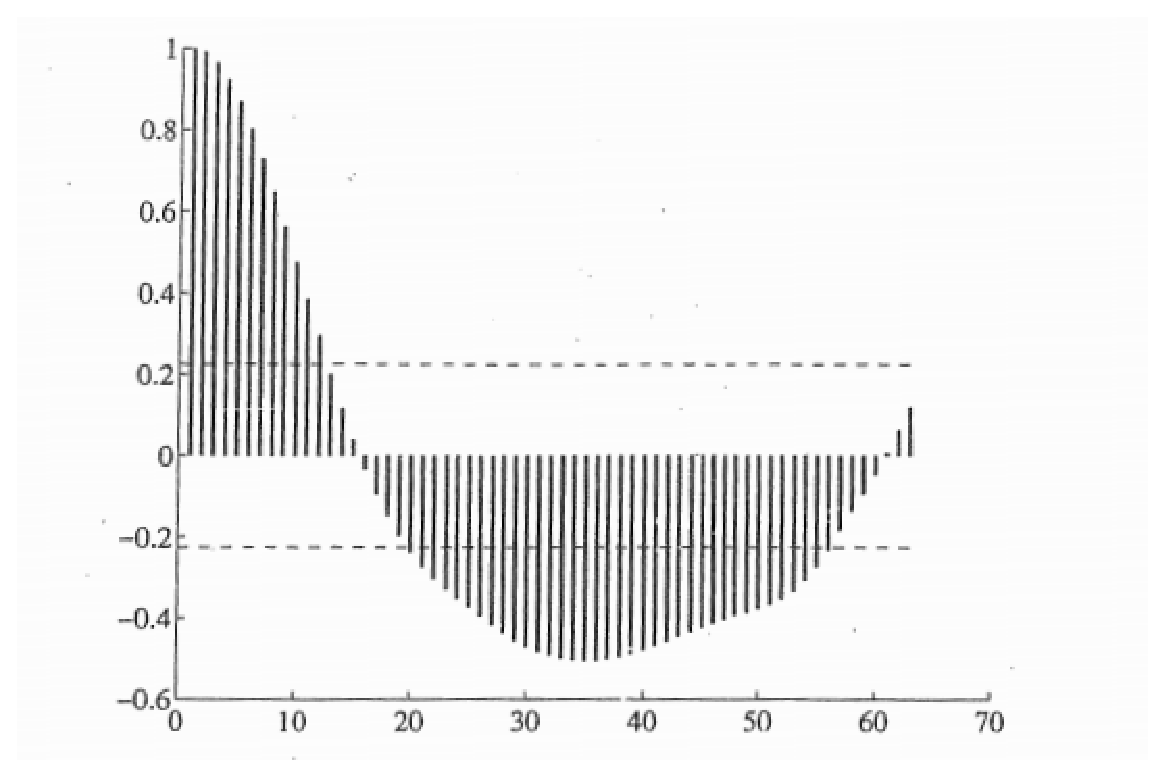
\includegraphics[width=0.7\linewidth]{TeX_files/Part02/chapter05/image/5}
	\caption{Correlogram for an autocovariance function. The dashed horizontal lines represent the limits $ \pm2/\sqrt{n},n $being 80.}
	\label{ }
\end{figure}
图5.5自协方差函数的相关图。 虚线水平线表示极限为$ \pm2/\sqrt{n},n $为80。
\subsection{方差分量模型}

我们再次假设我们的观察(信号)是静止的。 此外,在等距离时间反演中进行了观察。下面将介绍一些分析自相关函数的有用工具。

我们经常会提供标准化的自相关函数。 自相关系数 $ r_{k} $ 定义为

\begin{equation}\label{5.35}
r_{k}=\Re_{x}(k)/\Re_{x}(0),\quad k=0,1,...,n-1 
\end{equation}

变化k的图 $ r_{k} $ 被称为随机过程  $ x_{k} $ 的相关图。 相关图的一个简单的作用是检查观察时间序列中是否存在任何连续依赖性的证据。 为了做到这一点,我们使用一个结果,由于Bartlett表明,对于白噪声序列 $ a_{k} $,对于大的 $ n $,$ r_{k}  $大致正态分布,平均值为零,方差为 $  1 / n $。 因此,
大于 $ 2/\sqrt{n} $ 绝对值的  $ r_{k} $ 值可以在约5%的水平被认为是重要的。 如果计算大量数据  $ r_{k} $ ,即使ajc是白噪声序列,也有可能某些数值超过该阈值。

图5.5显示了接收机时钟偏移的相关图。 从0到12的偏移量超过极限值 $ ± 2/\sqrt{n} $,从$  k = 20 $ 到 $ k = 56 $。相关图表明观测值之间的相关性,即使是高达56个单位时间的变化。

在实践中,随机过程通常显示非随机趋势。 随着噪声 $ \epsilon_{t} $ 我们有

\[ Z_{t}=\mu_{t}+\epsilon{t} \]

我们将通过将第i个系列的观测值 $ Z_{i}(t) $ 分为起始水平  $ L_{i}(t) $ ,随机静止部分 $ M_{i}(t) $ 和噪声 $ N_{i}(t) $ 来演示如何处理这种情况:

\begin{equation}\label{5.36}
Z_{t}(t_{k})=L_{i}(t_{0})+M_{i}(t_{k})+N_{i}(t_{k})
\end{equation}

所有实验对象 $  i = 1,2,...,m $ 的所有观察值在等距离时间  $ t_{0},t_{1},...t_{k},L_{i} $ 被取代,随机变量取决于时间  $ t_{k} $ 时  $ L_{i} $ 在时间 $ t_{0} $  被定义。 $ i\neq j $时  $ L_{i} $独立于 $ L_{j} $,分布为  $ N(0,\lambda^{2}) $ 。 噪音分布为 $ N(0,\nu^{2}) $ ,在时间和主体之间独立。 最终 $ M_{i}(t_{k}) $ 分布为 $ N(0,\mu^{2}) $ ,当$ R(k)=\mu^{2}r(k) $ 和主体之间独立。 我们记得$ r(0) = 1 $和 $ r(k)\rightarrow 0 $时,$ k\rightarrow \infty $。 三个分量 $  L_{i},M_{i}, $和$ N_{i} $ 假定相互独立。观测方差为

\[ R_{Z}(0)=Var(Z_{i}=\lambda^{2}+\mu^{2}+\nu^{2}) \]

$ Z_{i}(t_{l}) $ 和  $ Z_{j}(t_{m}) $ 之间的协方差为


\begin{equation*}
\begin{aligned}
\sigma (Z_{i}(t_{i}), Z_{j}(t_{m}))&=E\left\lbrace Z_{i}(t_{i}) Z_{j}(t_{m})\right\rbrace\\
&=E\left\lbrace(L_{i}(t_{0})+M_{i}(t_{l})+N_{i}(t_{l}))(L_{j}(t_{0})+M_{j}(t_{m})+N_{j}(t_{m}))  \right\rbrace\\
&= E\left\lbrace L_{i}L_{j}\right\rbrace +E\left\lbrace M_{i}(t_{l})M_{j}(t_{m}) \right\rbrace =(Var(L_{i})+\mu^{2}r_{Z}(t_{m}-t_{l}))\delta_{ij}
\end{aligned}
\end{equation*}

注意,由于受试者的独立性,特别是 $ i\neq j $ 时协方差为零。

有一段时间我们对自相关 $ R_{Z}{k} $ 进行了研究。观测误差 $ N_{i}(t_{k}) $ 不等于零; 这意味着  $ k\rightarrow 0 $ 时 $ R_{Z}(k) $ 不接近 $ R_{Z}(0) $ ,$ k\rightarrow \infty $时$ R_{Z}(k) $ 也不接近0。 这是由主题特定的随机变量引起的。


从(5.34)我们记得R,并且E表示一个对角线元素都是1的矩阵,则协方差矩阵可以写为

 \[ \sum = \lambda^{2}E+\mu^{2}R+\nu^{2}I \]
 
 现在我们准备介绍变异函数了
 
 
 \begin{equation}\label{5.37}
V(k) = 1/2E\left\lbrace (Z_{i}(t_{l})-Z_{i}(t_{m}))^{2} \right\rbrace
\end{equation}

 
 我们有
 
  \[ Z_{i}(t_{l})-Z_{i}(t_{m})=M_{i}(t_{l})-M_{i}(t_{m})+N_{i}(t_{i})-N_{i}(t_{m})\]
  
  并记住, $ M_{i} $ 和 $ N_{i} $是独立的。
  
 \begin{equation*}
 \begin{aligned}
 V(k)&=1/2E\left\lbrace (M_{i}(t_{l})-M_{i}(t_{m}))^{2}\right\rbrace+1/2E\left\lbrace (N_{i}(t_{l})-N_{i}(t_{m}))^{2}\right\rbrace\\
 &=\mu^{2}(1-r_{Z}(k))+\nu^{2} 
 \end{aligned}
 \end{equation*}
  

图5.6显示了具有三个方差分量$ \lambda^{2},u^{2} $ 和 $ \mu^{2} $.的变异函数。 记住 $ r_{Z}(0)=1 $,因此 $ lim_{k\rightarrow 0}V(k)=\nu^{2} $。我们可以从图中读取 $ \nu^{2} $ 作为纵坐标轴的截距。

对于我们所用的任何静态,随机过程, $ k\rightarrow 0 $ 时我们有$ r_{Z}(k)\rightarrow 0 $ 。 因此$ V(\infty)=\mu^{2}+\nu^{2} $ 。 因此,个别受试者的差异  $\mu^{2} $ 被发现是$ V(\infty) $ 减去 $ \mu^{2} $。
\begin{figure}[h]
	\centering
	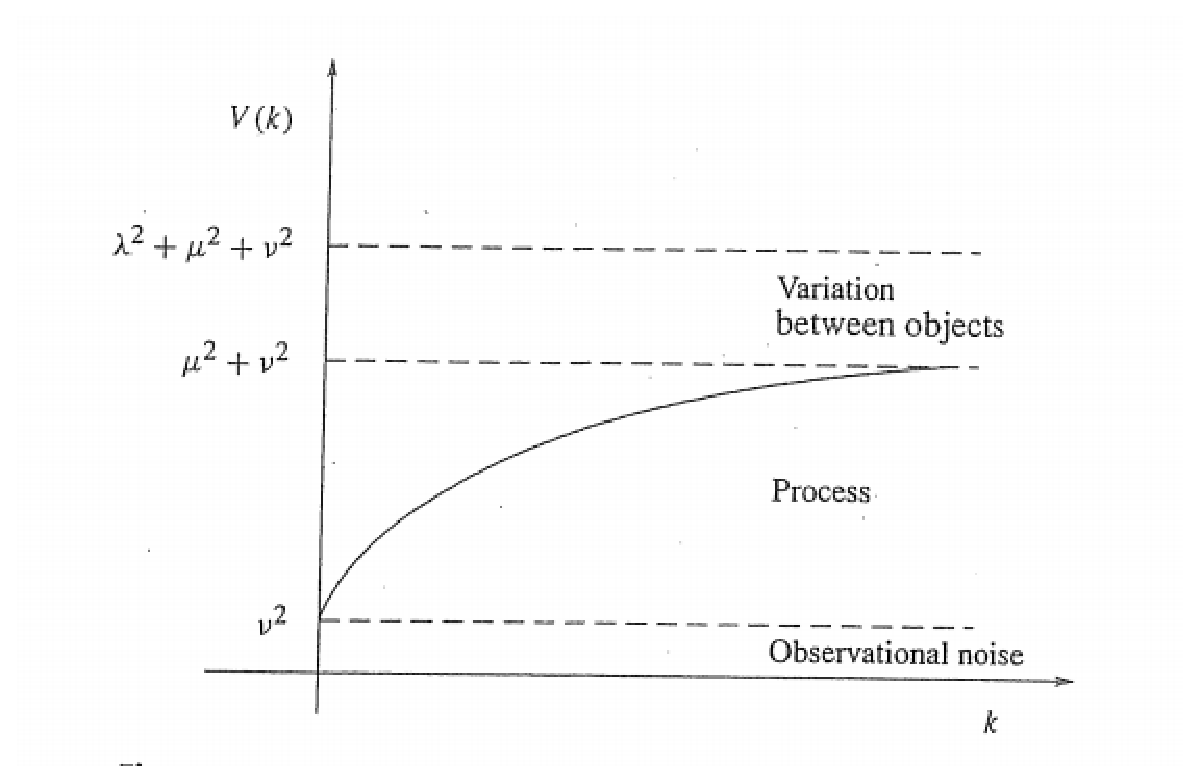
\includegraphics[width=0.7\linewidth]{TeX_files/Part02/chapter05/image/10}
	\caption{Variogram illustrating the three variance components}
	\label{ }
\end{figure}

通过实验对象的数据估计所有观测值$ Z_{i} $的总方差,再次假设过程相互独立,当 $ i\neq j $时,对所有的 $ l ,m,i和j$,总方差被计算为$ (Z_{i}(t_{l})-Z_{j}(t_{m}))^{2}/2 $的均值。这使得  $ M=\sum\nolimits_{i}(_{2}^{n_{i}}) $,其中,$ n_{i} $ 是 $ i $ 序列的观测次数:

 \[ \lambda^{2}+\mu^{2}+\nu^{2}=1/2M \sum_{i\neq j}(Z_{i}(t_{l})-Z_{j}(t_{m}))^{2} \]
 
 总方差如图6所示,人口的方差 $ \lambda^{2} $ 也可以在纵坐标轴中读取。
 
 自相关函数的两个常见例子是指数相关函数
 
\begin{equation}\label{5.38}
r(k)=e^{-\alpha k}
\end{equation}

 和高斯相关函数
 
\begin{equation}\label{5.39}
r(k)=e^{-\alpha k^{2}}
\end{equation}

 
 在图5.7中,我们绘制了(5.38)和(5.39)的自相关函数以及相应的变差函数。 对于小的时间差k,指数相关函数的相关性迅速降低,而高斯相关函数在较大时间内具有强相关性,后迅速下降。
 
 示例5.16为了演示该理论,我们使用接收机和卫星之间作单差。 我们使用具有伪随机噪声码(PRN)2,9,16,23,26和27号卫星。我们集中研究历元k的电离层延迟。我们使用双频观测值以消除延迟$ I_ {k} $中的主要误差:
 
  
 \[ I_{k} =\frac{(\Phi_{2,k}-\lambda_{2}N_{2})-(\Phi_{1,k}-\lambda_{1}N_{1})}{1-(f_{1}/f_{2})^{2}} \]
 
 
\begin{figure}[h]
	\centering
	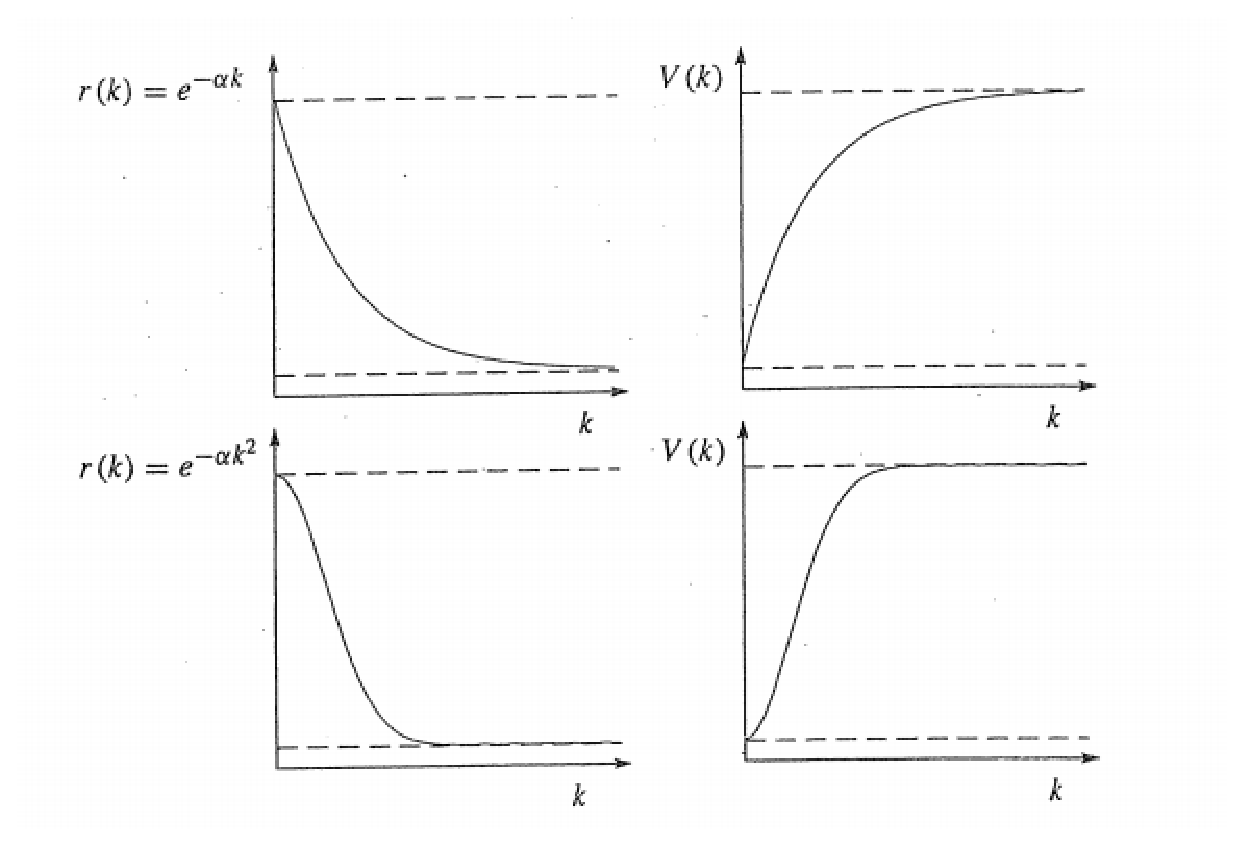
\includegraphics[width=0.7\linewidth]{TeX_files/Part02/chapter05/image/6}
	\caption{Exponential and Gaussian autocorrelationfunctions and variograms}
	\label{ }
\end{figure}

 
 图5.8描述了对于单差的$ I_ {k} $,单差再作差又是所谓的双差。实际基线长度为4.6公里。 对于单差 $ I_ {k} $ 通常在 $ 5-15 $ 米之间变化。 单差的 $ I_ {k} $ 值为2.5-3m,双差为 $ -0.2-0.2 $ 米。 请注意,单个PRN的仰角平均值列于表5.3。 我们可以看到到 $ I_ {k} $ 强烈地依赖于单个卫星的高度角。
 
 现在我们来看 $ I_ {k} $ 的自相关函数。为了消除观测序列中的可能趋势,经常会从历元差 $ I_ {K} -I_ {K-1} $ 开始调查 。图5.9(左上图)显示了2号卫星单差电离层延迟的自相关性。0处的峰值等于单差 $ I_ {K} -I_ {K-1} $ 的方差。现在我们计算非差的自相关性,结果
 
 \[\textbf{ Table 5.3} Autocorrelation of ionospheredelay for one-ways \] 
 \[ \begin{tabular}{lccc}
 \hline
 $ \quad$ & $ Elevation  $ & $\sigma_{1}(m)$&$Shift for firstzero  $ \\
 \cline{1-4}
 $ PRN$ & $ (^{\circ}) $ & $ master \quad rover $&$master \quad rover  $ \\
 $ 26$ & $ 68.9 $ & $ 0.08 \quad0.11 $&$35\quad 30  $ \\
 $ 2$ & $ 59.0 $ & $ 0.08 \quad0.04 $&$15\quad 35  $ \\
 $ 27$ & $ 28.0 $ & $ 0.39 \quad0.35 $&$30\quad 32  $ \\
 $ 16$ & $ 22.8 $ & $ 0.77 \quad0.71 $&$30\quad 30  $ \\
 $ 23$ & $ 20.4 $ & $ 0.17 \quad0.19 $&$12\quad 20  $ \\
 $ 9$ & $ 18.5 $ & $ 0.48 \quad0.19 $&$15\quad 30  $ \\
 
 \hline
 \end{tabular} \] 
 
 
 \begin{figure}[h]
 	\centering
 	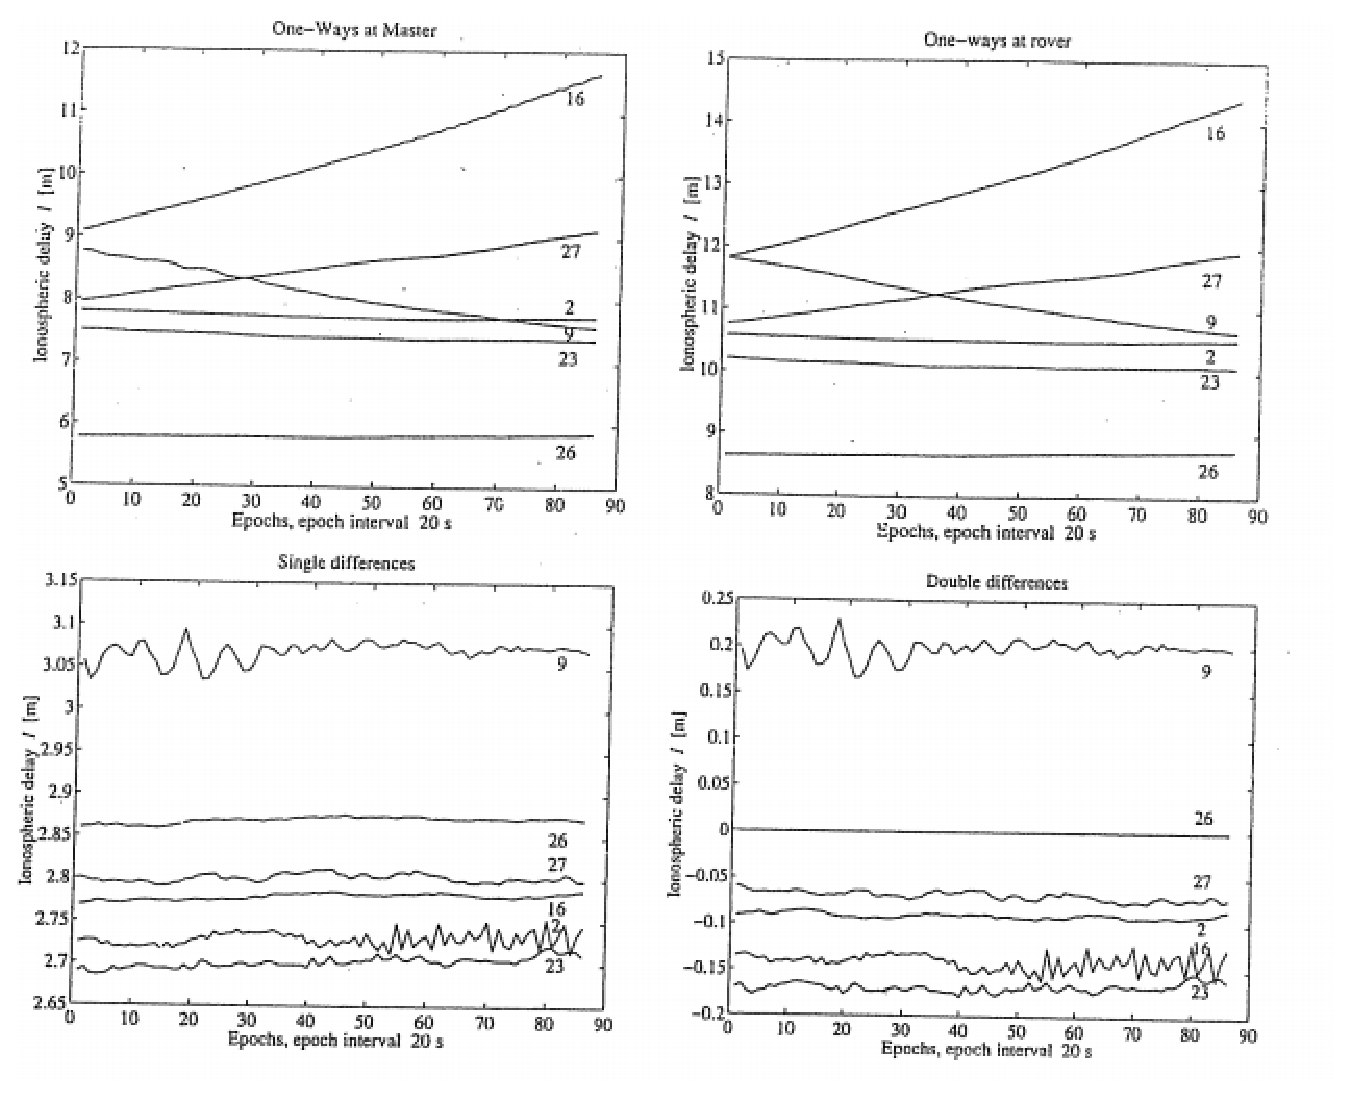
\includegraphics[width=0.7\linewidth]{TeX_files/Part02/chapter05/image/7}
 	\caption{Exponential and Gaussian autocorrelationfunctions and variograms}
 	\label{}
 \end{figure}
 
 如图右上方所示。这显然反应了延迟的系统性。我们的最终目标是对这部分进行建模,然后从实际延迟中减去,希望只留下白噪声或近似白噪声。有一个好的模型,我们可以提高电离层时间延迟 $ \ delta_ {t} $ 以及伪距 $ d $ 估计的精度。
 
 我们继续计算单差中  $ I_{k} $  的自相关值,计算单差的自相关值时必须遵守(5.13)给出的规则,这意味着我们必须计算互相关,图的左下角显示了2号卫星的结果。
 
 从表格5.3中我们得到2号卫星 $ \sigma_{1}=2 $厘米,16号卫星$ \sigma_{1}=77 $厘米,表5.3中的结果是通过调用下列函数产生的:
  \[ one_way(m)(27)\quad and \quad autocorr(x(2,:)^{'}) \]
  
  然而单差的结果减小到4毫米到9毫米,双差的结果减小到2毫米到9毫米,这个例子常用的M文件被称为$ oneway_{i} $。
  
  由于几何变化, $ I_{k} $ 会随着基线长度 $  d = 5, 25, 50, 100,500, 1000 $ 千米而变化,因此,我们建议有兴趣的读者进行探索和调查,最终确定差分电离层的方差 $ \sigma_{0}^{2} $ ,相关时间 $  T  $ ,相关长度 $ D $的关系。
  
  \begin{figure}[h]
  	\centering
  	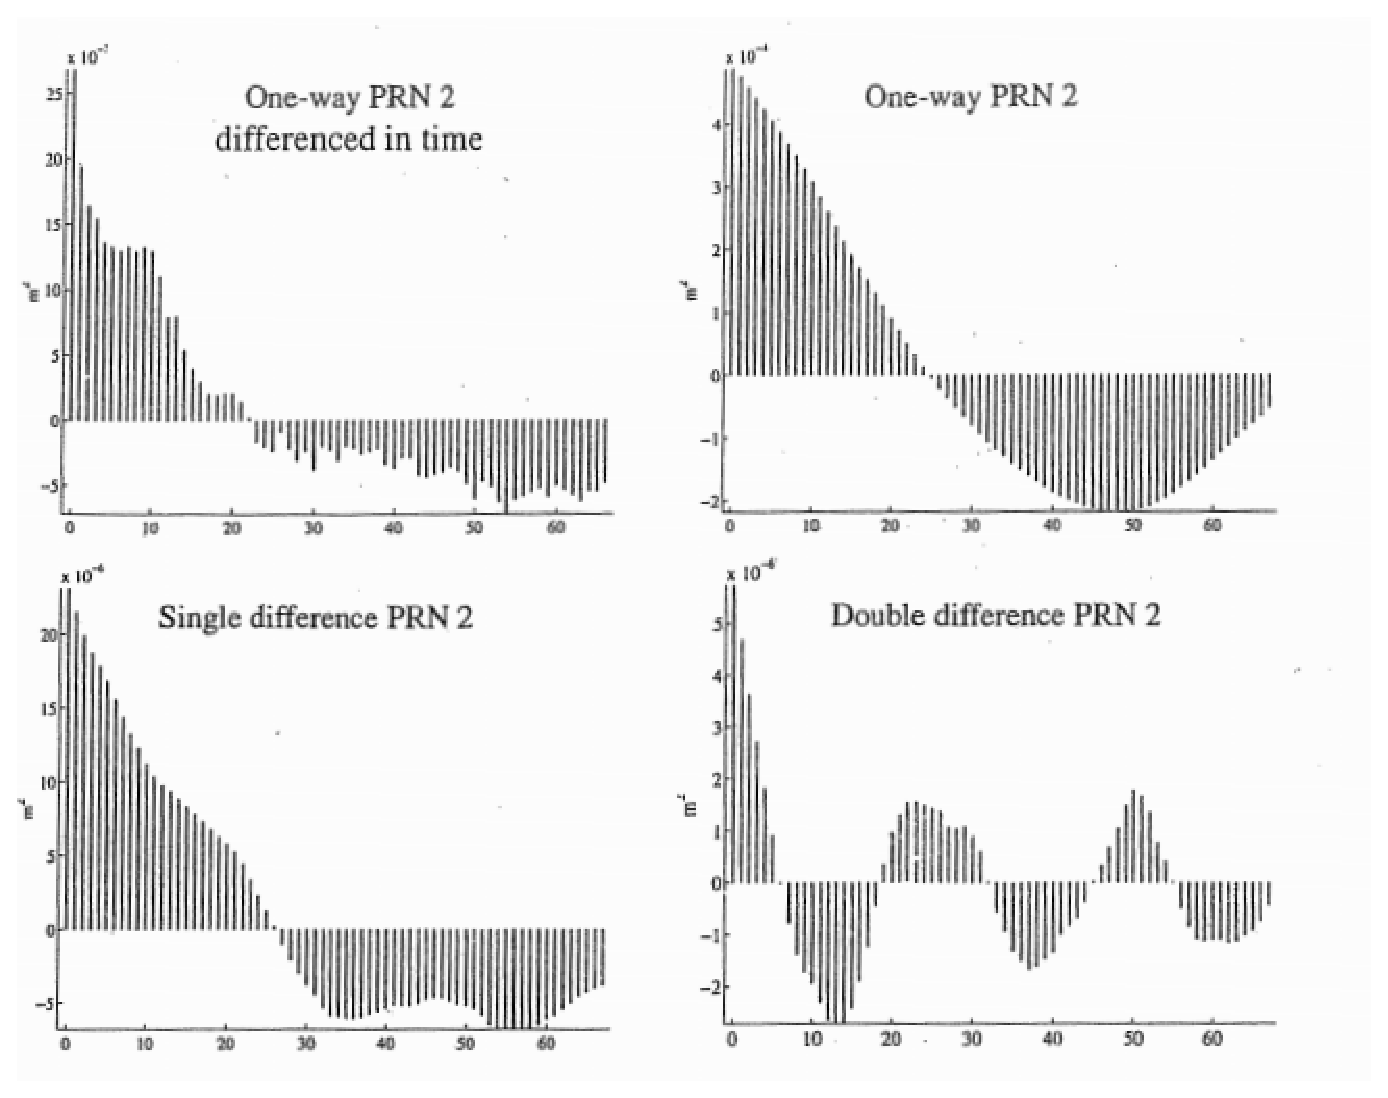
\includegraphics[width=0.7\linewidth]{TeX_files/Part02/chapter05/image/8}
  	\caption{Autocorrelation fo rionospheric delay to PRN 2}
  	\label{ }
  \end{figure}
   图的左上角显示了历元差分的结果,右上角显示了单历元的结果,左下角显示了单差的结果,右下角显示了双差的结果。注意各种数量级,采样间隔 $ \delta_{t} $ 和基线长度 $ d $ 关系如下:
   
   \begin{equation}\label{5.40}
   R_{x}(k,d)=\sigma_{0}^{2}e^{-|\delta_{t}|/T} e^{-d/D}
   \end{equation}
    
    这个函数 $ R_{x} $ 1994年由Goad和Yang通过载波的双差观测值提出。作者假设了一个平稳的指数相关过程:估计 $ T $ 到64分钟, $ \sigma_{0}^{2}=2m^{2} $, D $ \approx $ 1500千米,通常可以调整参数$ \sigma^{2} $和$ \alpha $来调整高斯——马尔科夫过程,在$ k = 0 $时调整$ \sigma_{0}^{2} $, 1/e时调整$ \alpha $。
    
    已知电离层延迟具有明显的日变化。 在Klobuchar(1996)中,我们发现以米为单位的 $ I $ 的近似表达式,作为当地时间 $ t $ 的函数 (以小时计):
    
    \[ I=2.1+0.75\cos((t-14)2\pi/28) \]
    
    该值在天顶方向有效。 为了获得$ I $的增加值,在高度角为1/2个周期的方向($ El $的范围为0-0.5,半个周期时间为$ \ pi $等于弧度),我们必须乘以倾斜因子。
    
     \[ F(El)=1+16(0.53-El)^{3} \]
     
     \begin{figure}[h]
     	\centering
     	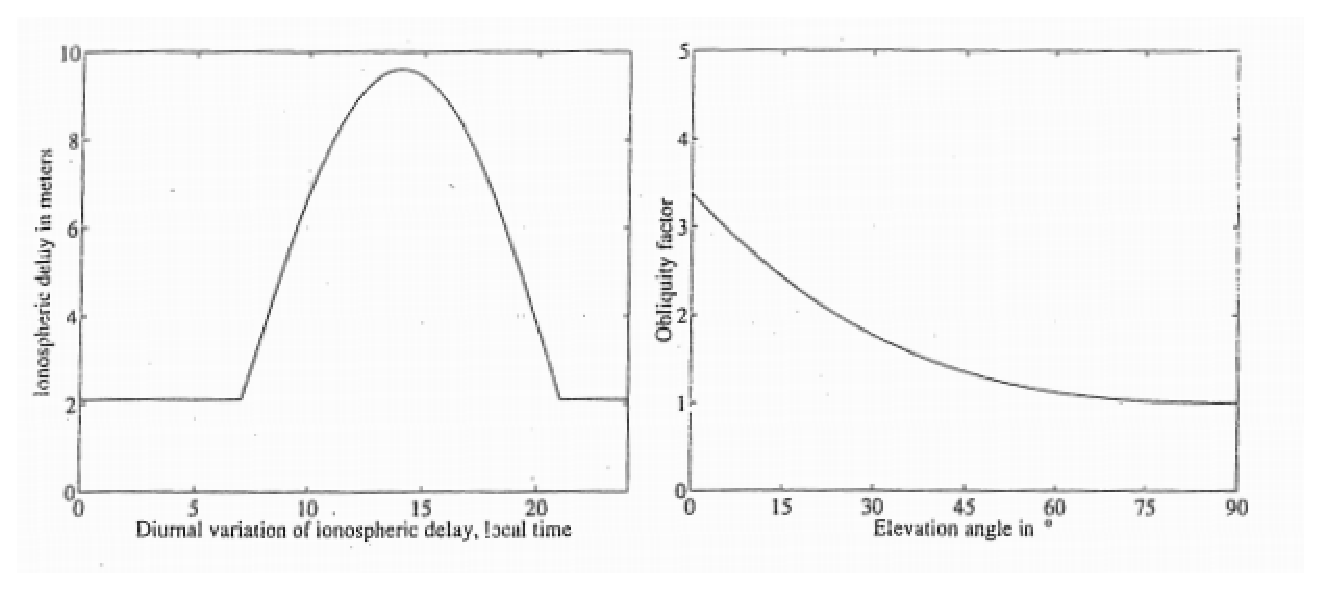
\includegraphics[width=0.7\linewidth]{TeX_files/Part02/chapter05/image/9}
     	\caption{Ionospheric delay model as function of local time and elevation angle}
     	\label{ }
     \end{figure}
     
     该表达式基于IS-GPS-200(2007)中给出的公式。 图5.10显示了$ I $和$ F(El)$的图表。小于2.1m的恒定的延迟表示夜间的延迟。 随着太阳升起,电离层延迟在白天呈现余弦形状。
     
     解释自相关函数时,请记住以下重要属性:
     
     最大值自相关函数的最大值为零移位:
     
      \[ E\left\lbrace x^{2}(t)\right\rbrace  = R_{x}(k) \]
      
      对称条件,自相关函数是一个偶数函数:
      
       \[ R_{x}(k) = R_{x}(-k) \]
       
       而互相关函数满足:
       
        \[ R_{xy}(k)=R_{yx}(-k) \]
        
        均方值互相关由下式决定:
        
         \[ |R_{xy}(k)|^{2}\leq R_{x}(0)R_{y}(0)\leq\frac{1}{2}((R_{x}(0))^{2}+(R_{y}(0))^{2}) \]
         
        周期性,如果 $ x $ 有周期性,则自相关函数也具有周期性。
        
       \textbf{ 备注5.1}(滤波差分技术的理论解释)我们可能会看到由两个单差测量数据 $ S_{i} $: $ D=S_{1}-S_{2} $组成的双差数据$ D $。每个单差测量数据都是简单的由 $ S_{i}=\rho_{i}+t $ 组成,其中 $ \rho_{i} $是伪距,$ t $是接收器时钟偏移乘以$ c $转换得到的长度。
       
       我们说明差分的几个基本事实。一开始有两个单差:
       
        \[ S_{1}=\rho_{1}+t \]
       \[ S_{2}=\rho_{2}+t \]
       
       和他们组成的双差
       
       \[ S_{2}-S_{1}=\rho_{2}-\rho_{1} \]
       
       对双差来说情况有所不同,双差不能估计$ t $,你可以从单差开始估计,但是先验钟差的方差  $ \sigma_{clock}^{2} $ 必须是无穷大,否则的话需要引入第三个观测量,但双差模型中没有。所以一个模型中要有$ S_{1} $, $ S_{2} $和 $ \sigma_{clock}^{2} $,这等价于$ S_{1} $, $ D $和  $ \sigma_{clock}^{2} $。 如果$ \sigma_{clock}^{2} = \infty $,这意味着它没有价值。所以等价于 $ S_{1} $ 和 $ D $。现在,双差不明确涉及钟差,$ S_ {1} $的唯一用途是估计钟差。由于双差不需要估计钟差,所以$ D $ 用来定位。
       
       然而,如果$ \ sigma_ {clock} ^ {2} <\ infty $,那么这将使这三个量结合在一起,在这种情况下,所有这三个测量都将一起处理。使用$S_{1},S_{2},t  $或$ S_{1},D,t $或 $ S_{2},D,t $都无关紧要。如果将时钟视为在每个历元都不同,然后绘制其估计值,您将看到时钟不会随无穷大的方差而漂移。 从理论上说,我们知道有关时钟漂移的一些事情是正确的,使用双差我们无法利用这些知识(因为t消除了)。
       
       现在无法回答的问题是“接收机时钟在什么程度上随机漂移?”明显不同的接收机具有非常大的差异(通常为石英)时钟。 国际地球动力学GPS服务(IGS)提出最好的办法是是用铷或甚至更好的铯振荡器驱动用于轨道计算的接收器。 甚至更好的是氢气,但现在他们太贵了,不予考虑。 那么具有较小方差的更具描述性的随机模型可以证明是有用的。 石英钟相对于厘米的定位要求漂浮得如此之大,试图对它们进行建模对改进位置几乎没有什么影响。所以我们可以得出结论:
       
       - 双重差异可以被认为是过滤器,其中钟差被建模为具有无限方差的白噪声。
       
       - 如果预测的方差小于无穷大,则使用单差分析预测接收机钟差比使用双差更好。
       
        \subsection{ 随机过程}
        
          我们提出了三个基本模型:随机游走,随机斜坡和指数相关过程。 每个模型都引入了一个特殊的模式,用于描述随机误差的相互作用。 如果模型被正建立择,则残差应为白噪声。对误差随机性的测量看其自相关性。 或者换句话说:给定的自相关函数基于给定的模型。 如果模型适合数据,误差自相关函数应该是是白噪声。
        
        
        纯粹的测量误差在零点会有很明显的峰值。系统误差会有一个很大的自相关性,即使远离零点。 为了演示随机数据的自相关,我们称之为M-file $ model_g $。结果如图5.4所示。 这里我们有一个自相关函数,在零点有一个峰值。 这个峰值是观察方差的一个量度。 自相关函数的全局特征(距离shift = 0)源于模型。 如果自相关在距零点一定距离后显著下降,我们会说这是一个受限过程。
        
        有时我们很幸运地知道一个问题背后的物理学知识。 然后通常用微分方程给出。
        
        \textbf{实例5.17} 我们描述一个过程,从微分方程开始 ,推出离散状态方程。 z变换显示结果的极点,这些极点决定滤波器是否稳定。
        
        实际的微分方程描述了一个过程的强制运动,质量为$ m $,阻尼常数$ d $,弹簧模量$ c $,均受到外力$ f $的影响 :
        
         \begin{equation}\label{5.41}
        m \ddot x + d \dot{x} +cx = f
        \end{equation}
        
        
        实际的位移是 $ x(t)=\int \ddot{x}(t)dt  $,我们区分得到 $ x_{k}\approx x_{k-1}+\dot{x}_{k-1} $  和  $ \delta_{t}=1 $。除此以外还有:
        
         \begin{equation}\label{5.42}
         \dot{x}(t)=\int \ddot{x} (t)dt \quad and \quad \dot{x}_{k}\approx\dot{x}_{k-1}+\ddot{x}_{k-1}
         \end{equation}
         
         方程(5.41)的离散形式是:
         
          \begin{equation}\label{5.43}
         \ddot{x}_{k-1}=- \frac{d}{m}\dot{x}_{k-1}-\frac{c}{m}x_{k-1}+\frac{f}{m}
         \end{equation}
         
         
         (5.43)插入(5.42)得到:
         
          \[ \dot{x}_{k}=\dot{x}_{k-1}+(- \frac{d}{m}\dot{x}_{k-1}-\frac{c}{m}x_{k-1}+\frac{f}{m}) \]
          
          因此,在矩阵形式中,状态方程成为:
          
           \[ \begin{bmatrix}
          x_{k}\\\dot{x}_{k}
          \end{bmatrix} = \begin{bmatrix}
          1&1\\-c/m&1-d/m
          \end{bmatrix} \begin{bmatrix}
          x_{k-1}\\\dot{x}_{k-1}
          \end{bmatrix}+\begin{bmatrix}
          0\\f/m
          \end{bmatrix}\]
          
          随机游走是$ c = 0 $和$ d = 0 $的特殊情况。 没有弹簧力,没有阻尼:
          
          \begin{equation}\label{5.44}
         \begin{bmatrix}
         x_{k}\\\dot{x}_{k}
         \end{bmatrix} = \begin{bmatrix}
         1&1\\0&1
         \end{bmatrix} \begin{bmatrix}
         x_{k-1}\\\dot{x}_{k-1}
         \end{bmatrix}+\begin{bmatrix}
         0\\f/m
         \end{bmatrix} 
         \end{equation}
          
          我们用 $ X_{1,k}=x_{k},X_{2,k}=\dot{x}_{k},F(z)=f/m $代替状态变量:
          
         \begin{equation}\label{5.45}
         \begin{bmatrix}
         X_{1,k}\\X_{2,k}
         \end{bmatrix} = \begin{bmatrix}
         1&1\\-c/m&1-d/m
         \end{bmatrix} \begin{bmatrix}
         X_{1,k-1}\\X_{2,k-1}
         \end{bmatrix}+\begin{bmatrix}
         0\\F(z)
         \end{bmatrix} 
         \end{equation}
          
          静态平衡的位移是$ X_{1,k} $, $ X_{2,k} $是瞬时速度。
          
          该离散系统的解决方案是通过z变换找到$ X_ {1}(z)= \ sum X_ {1,kz ^ { - k}} $和 $ X_{2}(z)=\sum X_{2,kz^{-k}} $。(5.45)的变换是:
          
            \[ zX_{1}(z)=X_{1}(z)+X_{2}(z) \]
          
          \[ zX_{2}(z)=-\frac{c}{m}X_{1}(z)+(1-\frac{d}{m})X_{2}(z)+F(z) \]
          
          我们重写最后的等式:
          \[ X_{2}(z)(z-(1-\frac{d}{m}))=- \frac{c}{m} X_{1}(z)+F(z) \]
          
          
          然后将  $ X2(z) $  插入到第一个方程中得到:
          
           \[ zX_{1}(z)=X_{1}(z)+\frac{-(c/m)X_{1}(z)+F(z)}{z-(1-d/m)} \]
           或
           \[ (z^{2}-(2-\frac{d}{m})z+(1-\frac{d}{m}+\frac{c}{m}))X_{1}(z)=F(z) \]
           
           位置 $ X_{1}(z) $ 由下式给出:
           
            \[ \frac{X_{1}(z)}{F(z)}=\frac{1}{z^{2}-(2-d/m)z+(1-d/m+c/m)} \]
           
           $ c = 0 $和$ d = 0 $的随机游走模型给出:
           
           \[ \frac{X_{1}(z)}{F(z)}=\frac{1}{z^{2}-2z+1}=\frac{1}{z-1}\frac{1}{z-1} \]

           
           函数 $ X_{1}(z) $ 在$ z = 1 $ 时具有多极点。 一般来说,如果所有极点都在单位圆内,我们将处理一个稳定的过滤器。 如果一个或多个极点在单位圆外,我们有一个不稳定的过滤器。$ z = 1 $在当前模型中是最细微的。 $ z = 1 $的邻域是一个真正的“雷区”。
           
           脉冲响应的z变换是转换函数 $ H (z) $。 输入和输出通过  $ H (z) $连接,它是最优控制的关键。 这进一步导致了自相关和光谱密度的显示。 然而,这个相对简单的例子是通过纯代数方法找到代数方程的闭合形式解的复杂性的极限。 所以我们不想提出更多的理论,因为在大多数现实世界中,是用数据而不是公式来描述现实。
           
           \textbf{实例5.8} 我们想在动态线性模型中组合随机游走和白噪声
           
           状态方程:$ x_{k}=x_{k-1}+\epsilon_{k},\epsilon_{k}~N_{1}(0,\sigma_{\epsilon}^{2})$
           观测方程:$ b_{k}=x_{k}+e_{k},e_{k}~N_{1}(0,\sigma_{e}^{2}) $
           
           这是最简单的模型,其应用范围非常广泛。
           
           我们通过重复高斯马尔可夫过程的要点来总结本章:
           
           自相关: $ \Re_{x}(k)=\sigma^{2}e^{-\alpha|k|} $
           过程:$ x_{k}=e^{-\alpha|\delta_{t}|}x_{k-1}+\epsilon_{k} $
           方差 $ \sigma_{\epsilon_{k}}^{2}=E\left\lbrace \epsilon_{k}^{2} \right\rbrace =\sigma^{2}(1-e^{-2\alpha|\delta_{t}|})$ 作用于过滤器的对角线
           协方差矩阵 $ \sum\nolimits_{\epsilon,k} $ ,参见第八章。
           
           
          
          
       
       
       
       
       
       


	
	%%----------------------------第五章结束-------------------------%%
		
	%%----------------------------第六章开始-------------------------%%
	\chapter[线性代数中加权最小二乘]{线性代数中加权最小二乘\\Linear Algebr for\\ Weighted Least Squares}
	\minitoc %小标题
	\newpage%新页
		\section[格瑞姆-史密正交化系数阵$A$和乔利斯基分解用于$A^{T}A$]{格瑞姆-史密正交化系数阵$A$和乔利斯基分解用于$A^{T}A$\\Gram-Schmidt on $A$ and Cholesky on $A^{T}A$}

		\section[计算正交矩阵]{计算正交矩阵\\Computing with Orthogonal Matrices}

		\section[奇异值]{奇异值\\Singular Value Decomposition(SVD)}
在本节中,我们要介绍新的坐标系统,其中最小二乘问题变得更简单,因此更加清晰。在坐标变换之后,我们说我们已经获得了最小二乘问题的“规范形式”,我们先介绍线性代数中的$SVD$,然后回到应用程序。

奇异值分解是线性代数的亮点。$A$是任何$m$乘$n$矩阵,正方形或矩形。它的秩是$r$。我们将对角线化这个$A$,但不是$S^{-1}AS$。$S$中的特征向量有三个大问题:它们通常不是正交的,并不总是有足够的特征向量,而且要求$A$为正方形。$A$的奇异向量以完美的方式解决所有这些问题。

我们付出的代价是有两套奇异向量,$\textbf{\textit{u}}$和$\textbf{\textit{v}}$。 $\textbf{\textit{u}}$是$AA^{T}$的特征向量,$\textbf{\textit{v}}$是$A^{T}A$的特征向量。由于这些矩阵都是对称的,因此它们的特征向量可以选择正交。在下面的等式(6.14)中,$A$乘$A^{T}A$与$AA^{T}$乘$A$相同的简单事实将导致这些$\textbf{\textit{u}}$和$\textbf{\textit{v}}$的显着性质:
\begin{align}
" A \ \text{是对角矩阵}\  \textquotedblright \ \ \ 
A\textbf{\textit{v}}_{1}=\sigma_{1}\textbf{\textit{u}}_{1} \ \ 
A\textbf{\textit{v}}_{2}=\sigma_{2}\textbf{\textit{u}}_{2} \ \cdots \ 
A\textbf{\textit{v}}_{r}=\sigma_{r}\textbf{\textit{u}}_{r}
\end{align}
奇异向量$\textbf{\textit{v}}_{1},\cdots,\textbf{\textit{v}}_{r}$ 在$A$的行空间中。输出$\textbf{\textit{u}}_{1},\cdots,\textbf{\textit{u}}_{r}$在$A$的列空间中。奇异值$ \sigma_{1},\cdots,\sigma_{r}$都是正数。当$\textbf{\textit{v}}$和$\textbf{\textit{u}}$进入$V$,$U$的列时,正交性给出$V^{T}V=I$和$U^{T}U=I$。$Q$进入对角矩阵$D$.

正如$ A\textbf{\textit{x}}_{i}=\lambda_{i}\textbf{\textit{x}}_{i}$引出对角化$AS=S\Lambda$,方程$A\textbf{\textit{v}}_{i}=\sigma_{i}\textbf{\textit{u}}_{i}$逐列告诉我们$AV = UD$:
\begin{align}
\begin{array}{l}
(m \ \times \ n)(n \ \times \ r) \\
\ \text{=} \\              
(m \ \times \ r) (r \ \times \ r)
\end{array}  A
\begin{bmatrix}
\ \\
\textbf{\textit{v}}_{1} \ \cdots \ \textbf{\textit{v}}_{r}\\
\ 
\end{bmatrix}=
\begin{bmatrix}
\ \\
\textbf{\textit{u}}_{1} \ \cdots \ \textbf{\textit{u}}_{r}\\
\ 
\end{bmatrix}
\begin{bmatrix}
\sigma_{1}  & & \\
& \ddots &\\
& & \sigma_{r} 
\end{bmatrix}
\end{align}
这是$SVD$的核心,但还有更多。这些$\textbf{\textit{v}}$和$\textbf{\textit{u}}$说明了$A$的行空间和列空间。我们需要从零空间$ \textbf{N}(A)$和左零空间$ \textbf{N}(A^{T})$得到$n-r$个更多的$\textbf{\textit{v}}$和$m-r$个更多的$\textbf{\textit{u}}$。它们可以是这两个空间的正交基(然后自动正交于第一个$r$ $\textbf{\textit{v}}$和$\textbf{\textit{u}}$的)。包括所有在$V$和$U$的$\textbf{\textit{v}}$和$\textbf{\textit{u}}$,所以这些矩阵变成方阵。我们仍然有$AV = UD$。
\begin{align}
\begin{array}{l}
(m \ \times \ n)(n \ \times \ n) \\
\text{equals} \\              
(m \ \times \ m) (m \ \times \ n)
\end{array}  A
\begin{bmatrix}
\ \\
\textbf{\textit{v}}_{1} \ \cdots \ \textbf{\textit{v}}_{r} \ \cdots \textbf{\textit{v}}_{n}\\
\ 
\end{bmatrix}=
\begin{bmatrix}
\ \\
\textbf{\textit{u}}_{1} \ \cdots \ \textbf{\textit{u}}_{r} \ \cdots \textbf{\textit{u}}_{m}\\
\ 
\end{bmatrix}
\begin{bmatrix}
\sigma_{1}  & & &\\
& \ddots & &\\
& & \sigma_{r} & \\
& & & & 
\end{bmatrix}
\end{align}
新的$D$是$m$乘$n$。它只是旧的$r$乘$r$矩阵(称为$D_{r}$),其中$m-r$个新的零行和$n-r$个新的零列。真实的变化是$U$和$V$和$D$的形状.而且$V^{T }V = I$和$U^{T }U=I$,大小为$n$和$m$。

$V$现在是正方形正交矩阵,具有逆$V^{-1}=V^{T}$。因此$AV=UD$可以变为$A=UDV^{T}$。这是奇异值分解:
\begin{align}
SVD & &  A=UDV^{T}=\textbf{\textit{u}}_{1}\sigma_{ 1}\textbf{\textit{v}}^{T}_{1}+\cdots+\textbf{\textit{u}}_{r}\sigma_{ r}\textbf{\textit{v}}^{T}_{ r}
\end{align}
我们将早期的“减少的$SVD$”从等式($6.10$)写为$A=U_{r}D_{r}V^{T}$。这同样是真的,在$D$中没有额外的零。这个减少的$SVD$给出了$A$的相同的分裂为$r$个矩阵的总和,每个矩阵的秩为1。

我们将看到$ \sigma^{2}_{i}=\lambda_{i}$是$A^{T}A$和$AA^{T}$的特征值。当我们按照降序排列奇异值时,,公式(6.12)中的分裂给出了重要性顺序中的$r$个一阶$A$.

示例6.2 $UDV^{T}$(奇异值)何时与$SAS^{-1}$(特征值)相同?

解:我们需要$S=U$中的正交特征向量。我们需要非负特征值$ \Lambda = D $。因此$A$必须是正半定式(或确定)对称矩阵$Q \Lambda Q^{T}$。

例6.3 如果$A=\textbf{\textit{x}}\textbf{\textit{y}}^{T}$单位矢量$\textbf{\textit{x}}$和$\textbf{\textit{y}}$,$A$的$SVD$是多少?

解决方案(6.10)中的减少的$SVD$恰好是$\textbf{\textit{x}}\textbf{\textit{y}}^{T}$,秩为1。它有$\textbf{\textit{u}}_{1}=\textbf{\textit{x}}$和$\textbf{\textit{v}}_{1}=y$和$\sigma_{1}=1$。对于完整的$SVD$,完成$\textbf{\textit{u}}_{1}=\textbf{\textit{x}}$到$\textbf{\textit{u}}$的正交基,并完成$\textbf{\textit{v}}_{1}=\textbf{\textit{y}}$到$\textbf{\textit{v}}$的正交基。没有新的$\sigma$。

矩阵$U$和$V$包含所有四个子空间的正交基:
\begin{align*}
&   &r&                &V\text{的列:}&          &A\text{的行空间} \\ 
&   &n-r&               &V\text{的列: }&         &A\text{的零空间 }\\
&   &r &               &V\text{的列:}&         &A\text{的列空间} \\
&   &m-r &             &V\text{的列:}&          &A^{T} \text{的零空间}.
\end{align*}
第一列$\textbf{\textit{v}}_{1},\cdots,\textbf{\textit{v}}_{r}$和$\textbf{\textit{u}}_{1},\cdots,\textbf{\textit{u}}_{r}$是$A^{T}A$和$AA^{T}$的特征向量。我们现在解释为什么$A\textbf{\textit{v}}_{i}$落在$\textbf{\textit{u}}_{i}$的方向。最后的$\textbf{\textit{v}}$和$\textbf{\textit{u}}$的(在零空间)更容易。只要那些向量是正交的,$SVD$将是正确的。

$SVD$的证明从$A^{T}A\textbf{\textit{v}}_{i}=\sigma^{2}_{i}\textbf{\textit{v}}_{i}$开始,它给出了$\textbf{\textit{v}}$和$\sigma$的值。乘以$ \textbf{\textit{v}}^{T}_{i}$得到$ \lVert A\textbf{\textit{v}}_{i} \lVert ^{2}$,为了证明$ A\textbf{\textit{v}}_{i}=\sigma_{ i}\textbf{\textit{u}}_{i}$,关键一步是乘以$A$:
\begin{align}
\textbf{\textit{v}}^{T}_{i}A^{T}A\textbf{\textit{v}}_{i}=\sigma^{2}_{i}\textbf{\textit{v}}^{T}_{i}\textbf{\textit{v}}_{i}  & & \text{令} & &     \lVert A\textbf{\textit{v}}_{i} \lVert^{2}=\sigma^{2}_{i}
&  & \text{所以} & & \lVert  A\textbf{\textit{v}}_{i} \lVert = \sigma_{i}
\end{align}
\begin{align}
AA^{T}A\textbf{\textit{v}}_{i}=\sigma^{ 2}_{i}A\textbf{\textit{v}}_{i} & & \text{令} & & \textbf{\textit{u}}_{i}=A\textbf{\textit{v}}_{i}/\sigma_{ i} & & \text{作为单位特征向量} & AA^{T}.
\end{align}
方程(6.13)使用了放置括号的小技巧在$(\textbf{\textit{v}}^{T}_{i}A^{T})(A\textbf{\textit{v}}_{i})=\lVert A\textbf{\textit{v}}_{i} \lVert ^{2}$。方程(6.14)将所有重要的括号放在$(AA^{T})(A\textbf{\textit{v}}_{i}) $中。这表明$A\textbf{\textit{v}}_{i}$是$AA^{T}$的特征向量。除以长度$\sigma_{i}$得到单位向量$\textbf{\textit{u}}_{i}=A\textbf{\textit{v}}_{i}/\sigma_{ i} $。

这完成了$SVD$背后的“理论”。

现在是应用!使线性化观测方程为
\begin{align}
A\textbf{\textit{x}}=\textbf{\textit{b}}
\end{align}
其中$\textbf{\textit{x}}$是描述对未知(坐标)的校正的$n$维向量,并且$\textbf{\textit{b}}$是观察的$m$维向量。它们被假定为不相关和相等的权重。换句话说,观察的协方差矩阵是$ \Sigma_{b}=I$。

奇异值分解$SVD$表明找到正交矩阵$V$(在$A$的行空间或坐标空间中)和正交$U$(在$A$或观察空间的列空间中)总是有效的,使得$U^{T}AV$是奇异值的对角矩阵$\sigma_{1},\sigma_{2},\cdots,\sigma_{r} $通常表示为$ \Sigma$,但我们使用$D$来区别协方差矩阵。现在将$\textbf{\textit{x}}$和$\textbf{\textit{b}}$更改为$\textbf{\textit{y}}$和$\textbf{\textit{c}}$:
\begin{align}
\textbf{\textit{x}}=V\textbf{\textit{y}}  \ \ \text{和} \ \ \textbf{\textit{b}}=U\textbf{\textit{c}}. 
\end{align}
\begin{flushleft}
	然后 $A \textbf{\textit{x}}=\textbf{\textit{b}}$ 成为
\end{flushleft}
\begin{align}
B\textbf{\textit{y}}=\textbf{\textit{c}}
\end{align}
\begin{flushleft}
	\text{其中}
\end{flushleft}
\begin{align}
B=U^{T}AV
\end{align}
\begin{flushleft}
	 $SVD$ 选择 $U$ 和 $V$ 所以$ B$ 的形式是
\end{flushleft}
\begin{align}
B
\end{align}
\begin{flushleft}
	与对角矩阵$D$(通常称为$ \Sigma$,这里是协方差):
\end{flushleft}
\begin{align}
D=
\begin{bmatrix}
\sigma_{1}  & & &\\
& \sigma_{1} & &\\
& & \ddots & \\
& & & \sigma_{n} 
\end{bmatrix}.
\end{align}
矩阵$O$是($m-n$)乘$n$的矩阵。此外,奇异值按递减排序
\begin{align*}
\sigma_{1}\geq \sigma_{2} \geq \sigma_{3} \ldots \geq \sigma_{n}\geq 0
& & 
(\text{假设} \ \sigma_{r+1} = 0) .
\end{align*}
显然我们有
\begin{align}
B^{T}B=VA^{T}U^{T}UAV^{T}=VA^{T}AV^{T}=D^{2}
\end{align}
和
\begin{align}
BB^{T}=UAV^{T}VA^{T}U^{T}=UAA^{T}U^{T}=
\begin{bmatrix}
D^{2} & \textit{O} \\
\textit{O} & \textit{O}
\end{bmatrix}
\end{align}
记住正交矩阵$Q$有$ Q^{T}Q=QQ^{T}=I$,现在,我们让
\begin{align}
V^{T}=(\varphi_{1},\varphi_{2},\cdots,\varphi_{n}),
\end{align}
和
\begin{align}
UT=(\psi_{1},\psi_{2},\cdots,\psi_{n},\rho_{1},\rho_{2},\cdots,\rho_{m-n}),
\end{align}
其中$ \{ \varphi_{i} \}  $表示$ A^{T}A $的特征向量的正交集合,并且$ \{\psi_{i}\}\cup\{\rho_{i}\}$是$AA^{T}$的特征向量的正交集合。等式(6.16)的转置版本表示$\textbf{\textit{y}}$可以被看作系数$\{\varphi_{i}\}$中的向量$\textbf{\textit{x}}$的扩展,并且相应地,$\textbf{\textit{c}}$包含在$ \{\psi_{i}\} $和$ \{\rho_{i}\} $的扩展中$\textbf{\textit{b}}$的系数。我们称$ \{\varphi_{i}\} $,$ \{\psi_{i}\} $和 $ \{\rho_{i}\} $为第一,第二和第三组标准向量,即使它们没有被唯一地确定。

最小二乘问题的规范形式的统计解释由Scheff$\acute{e}$ (1959)的第一章给出。$ \{\rho_{i}\} $向量所跨越的空间被称为误差空间,$ \{\varphi_{i}\} $是估计空间。

在(6.18)和(6.19)的基础上,我们显示下面的前两组规范向量之间的关系是有效的:
\begin{align}
A\varphi_{i}=\sigma_{i}\psi_{i}, & &  i=1,2,\cdots,n.
\end{align}
类似地,从(6.18)和(6.19)中
\begin{align}
A^{T}\psi_{i}=\sigma_{i}\varphi_{i}, & &  i=1,2,\cdots,n
\end{align}
\begin{align}
A^{T}\rho_{i}=0, & &  i=1,2,\cdots,m-n.
\end{align}
在$\textbf{\textit{b}}$的正交变换$U$中留下在(6.17)权重归一化的观察值$\textbf{\textit{c}}$,我们可以通过对角化的正规方程来求解最小二乘问题
\begin{align}
B^{T}B\textbf{\textit{y}}=B^{T}\textbf{\textit{c}}
\end{align}
或
\begin{align*}
\sigma^{2}_{i}y_{i}=\sigma_{i}c_{i}, & & i=1,2,\cdots,n  &  & \text{或}&  & y_{j}=\dfrac{c_{j}}{\sigma_{j}},& & j=1,2,\cdots,r
\end{align*}
其中A的秩$r$是非零$ \sigma_{j}'s $的数目,并且拉丁下标$j$表示这些向量$\textbf{\textit{y}}$和$\textbf{\textit{c}}$的分量。

 这些事实导致以下重要后果:

1 \ 关于第一组规范向量:最好确定的$\textbf{\textit{x}}$的组成部分是那些在$ \varphi_{i} $有着$ \sigma_{i} $定义的方向上的;有$ \sigma_{i}=0 $的$ \varphi_{i} $的条目完全不确定。

为了正确地解释该结果,必须在大致相同的单位中测量坐标的校正。通常希望 $\textbf{\textit{x}}$的所有条目以相同的精度确定。

2 \ 第二组显示应该用更大的权重执行观察。这是因为我们扩大了个人观察。举个例子,$ \{\psi_{i}\} $和$ \{\rho_{i}\} $中的单位向量,并随后选择具有主导系数并且$ \sigma_{i}\neq0 $。这些系数可以通过检查矩阵$U$来找到。这是属性$U^{T}U=I$的结果,其也可以被视为产生单位向量扩展成集合的$ \{\psi_{i}\} $ 和$ \{\rho_{i}\} $。

3 \ 对于第三组,我们认识到在$ \{\rho_{i}\} $确定的方向上的观察项的条目不给出关于坐标的任何新的信息。这也适用于$ \psi_{i} $,其中$i>r$,即对应于奇异值的奇异向量$ \sigma_{i}=0 $。定义第$i$次观测的冗余可能是相关的
\begin{align}
red_{i}=\sqrt{p = \sum_{j=r+1}^mu^{2}_{ji}.}
\end{align}
 

		\section[条件数]{条件数\\The Condition Number}

		\section[对权重的依赖]{对权重的依赖\\Dependency on the Weights}
一个已经获得最小二乘问题基本知识的人很快提出这个问题:权重有多重要? 如果我们改变他们有点多少,这改变了解决方案? 让我们试着得到一些洞察的问题。 像往常一样,我们从一组观测方程$ A\textbf{\textit{x}}=\textbf{\textit{b}}-\textbf{\textit{e}} $和权重矩阵$C$开始。

我们将观察向量$\textbf{\textit{b}}$分成两个子向量。首先,我们对$\textbf{\textit{b}}_{1}$和$\textbf{\textit{b}}_{2}$的尺寸没有限制。向量$\textbf{\textit{e}}$和矩阵$A$和权重$C$
\begin{align*}
\textbf{\textit{b}}=
\begin{bmatrix}
\textbf{\textit{b}}_{1} \\	
\textbf{\textit{b}}_{2}
\end{bmatrix},
\quad
\textbf{\textit{e}}=
\begin{bmatrix}
\textbf{\textit{e}}_{1} \\	
\textbf{\textit{e}}_{2}
\end{bmatrix},
\quad
A=
\begin{bmatrix}
A_{1} \\	
A_{2}
\end{bmatrix},
\quad
C=
\begin{bmatrix}
C_{1} & 0\\	
0   & C_{2}
\end{bmatrix}.
\end{align*}
这意味着在两组观察之间没有权重耦合。原来的问题变成两个明显的问题:
\begin{align*}
A_{1}\textbf{\textit{x}}&=\textbf{\textit{b}}_{1}-\textbf{\textit{e}}_{1}  &\text{权阵} \ C_{1}                      \\
A_{2}\textbf{\textit{x}}&=\textbf{\textit{b}}_{2}-\textbf{\textit{e}}_{2}  &\text{权阵} \ C_{2}    
\end{align*}
并且我们可以计算每个系统的解。现在有趣的问题是:这些解决方案与整个问题的解决方案相比有什么表现?

我们将看到当我们将第二组的权重$C_{2}$改变为$ C_{2}+\delta C_{2}$时,解$\hat{\textbf{\textit{x}}}$的误差$ \delta \textbf{\textit{x}} $是多少。$ \delta \textbf{\textit{x}} $的表达式涉及一个有用矩阵公式的矩阵计算。原始问题的正规方程是
\begin{align*}
\begin{bmatrix}
A^{T}_{1} &	A^{T}_{2}
\end{bmatrix}
\begin{bmatrix}
C_{1} &	0 \\
0     &	C_{2}
\end{bmatrix}
\begin{bmatrix}
A_{1} \\
A_{2}
\end{bmatrix}  \hat{\textbf{\textit{x}}} = 
\begin{bmatrix}
A^{T}_{1} &	A^{T}_{2}
\end{bmatrix}
\begin{bmatrix}
C_{1} &	0 \\
0     &	C_{2}
\end{bmatrix}
\begin{bmatrix}
\textbf{\textit{b}}_{1} \\
\textbf{\textit{b}}_{2}
\end{bmatrix}.
\end{align*}
这可以写成
\begin{align}
(A^{T}_{1}C_{1}A_{1}+A^{T}_{2}C_{2}A_{2})\hat{\textbf{\textit{x}}}=A^{T}_{1}C_{1}\textbf{\textit{b}}_{1}+A^{T}_{2}C_{2}\textbf{\textit{b}}_{2}.
\end{align}
注意如何收集来自两个问题的正规方程。对正态方程的贡献具有可加性特征。扰动的问题是
\begin{align}
(A^{T}_{1}C_{1}A_{1}+A^{T}_{2}(C_{2}+\delta C_{2} )A_{2})(\hat{\textbf{\textit{x}}}+\delta \textbf{\textit{x}} )=(A^{T}_{1}C_{1}\textbf{\textit{b}}_{1}+A^{T}_{2}(C_{2}+\delta C_{2} )\textbf{\textit{b}}_{2}).
\end{align}
现在从(6.32)中减去(6.31),得到$ \delta \textbf{\textit{x}} $的方程:
\begin{align}
(A^{T}_{1}C_{1}A_{1}+A^{T}_{2}(C_{2}+\delta C_{2} )A_{2})\delta \textbf{\textit{x}} + A^{T}_{2}\delta C_{2}A_{2}\textbf{\textit{x}}=
A^{T}_{2}\delta C_{2}\textbf{\textit{b}}_{2}.
\end{align}
我们令$ N= A^{T}_{1}C_{1}A_{1} + A^{T}_{2}C_{2}A_{2}$和$ \hat{\textbf{\textit{e}}}_{2} = \textbf{\textit{b}}_{2} - A_{2}\textbf{\textit{x}}  $。那么$\hat{\textbf{\textit{x}}}$的变化是
\begin{align}
\delta \textbf{\textit{x}} = ( N + A^{T}_{2}\delta C_{2}A_{2})^{-1}
A^{T}_{2}\delta C_{2} \hat{\textbf{\textit{e}}}_{2}.
\end{align}
下面的重要公式,取自(8.45),得出:
\begin{align}
( N + A^{T}_{2}\delta C_{2}A_{2})^{-1} = N^{-1} - N^{-1}A^{T}_{2}
(A_{2}N^{-1}A^{T}_{2} +(\delta C_{2})^{-1} )^{-1} A_{2} N^{-1}
\end{align}
对于$n$个观测值,该矩阵乘以$ A^{T}_{2}\delta C_{2} \hat{\textbf{\textit{e}}}_{2} $得到$ \delta \textbf{\textit{x}} $。如果我们专注于一个单一的观测值,$ A^{T}_{2} $成为一个$n$乘1矩阵, $ \delta C_{2} $是1乘1.我们命名$ A_{2}N^{-1}A^{T}_{2} = s $并且得到
\begin{align*}
\delta \textbf{\textit{x}} = N^{-1} A^{T}_{2} (1-\dfrac{\delta C_{2}}{1+s\delta C_{2}}s)\delta C_{2}\hat{e}_{2}
\end{align*}
或
\begin{align}
\delta \textbf{\textit{x}} = \dfrac{\hat{e}_{2}\delta C_{2} }{1+s\delta C_{2}}N^{-1}A^{T}_{2}.
\end{align}
表达式(6.36)揭示了几个有趣的事实。解决方案中的变化 $ \delta \textbf{\textit{x}} $(一阶近似)与权重变化$ \delta C_{2} $成正比。在与$A_{2}$中包含的观察相关的未知数中,$ \delta \textbf{\textit{x}} $变化最大。$ N^{-1}A^{T}_{2} $只有来自$N^{-1}$的列的贡献,该列对应于不同于零的$ A^{T}_{2} $。

已经在1823年C.F.高斯找到一个单一权重$ \delta C_{2} $的变化的类似表达式。参见高斯(1995)中的“更新观察变化的未知数”一节。

\begin{figure}[htb]
	\centering
	\includegraphics[width=0.7\linewidth]{TeX_files/Part02/chapter06/image/6-1}
	\caption{Dependence of $ \hat{\textbf{\textit{x}}}$ on $ \delta C_{2}$ \text{在实例} 6.4}
\end{figure}

实例6.4 \ 我们想要演示关于简单最小二乘问题的过程:
\begin{align*}
A = 
\begin{bmatrix}
1&1 \\	
1&2 \\		
-1&1 	
\end{bmatrix} \quad 
\text{和} \quad 
\textbf{\textit{b}}=
\begin{bmatrix}
2 \\	
1 \\		
0 	
\end{bmatrix} \quad 
\text{和} \quad 
C+\delta C_{2} =
\begin{bmatrix}
1   &   & \\	
&   2   & \\		
&   &  1+\delta C_{2} 	
\end{bmatrix} 
\end{align*}
然后$ \delta C_{2} =0 $照常产生解$\hat{\textbf{\textit{x}}}$和残差向量$\hat{\textbf{\textit{e}}}$:
\begin{align*}
\hat{\textbf{\textit{x}}} = \dfrac{1}{3}
\begin{bmatrix}
2 \\	
1 	
\end{bmatrix} \quad 
\text{和} \quad 
\hat{\textbf{\textit{e}}} = \dfrac{1}{3}
\begin{bmatrix}
3 \\	
-1 \\
1	
\end{bmatrix}.
\end{align*}
令$\delta C_{2} =-1 $对应于消除第三观测量。然后$ \hat{\textbf{\textit{x}}}=(3,-1)$是前两行的交点。我们得到第三行元素从(3,-1)到(5/11,5/11)的线段,随着$\delta C_{2} $从-1到$ \infty$。所有权重变化,我们显然可以在三角形内的任何地方获得解。

 $M$文件$dw$反映了发生了什么。
 
 这种权重变化的方法对于少量的观测是极好的。对于一个更大的问题的更多的定性知识,我们转向一个更强大的工具。

现在我们要求更多的定量结果:如果权重改变,投影$\textbf{\textit{p}}=P\textbf{\textit{b}}$在$A$的列空间中移动多少?这种运动的描述是
\begin{align}
tan \alpha = \dfrac{\rVert \textbf{\textit{p}}_{2} - \textbf{\textit{p}}_{1}\rVert c_{1}}{\rVert \textbf{\textit{b}} - \textbf{\textit{p}}_{1}\rVert c_{1}}.
\end{align}
范数由$ \rVert \textbf{\textit{x}} \rVert c_{1}  = \rVert  C_{1}\textbf{\textit{x}} \rVert$加权,$ \alpha$是在行程$ \overline{\textbf{\textit{p}}_{1}\textbf{\textit{p}}_{2}}$处的$\textbf{\textit{b}}$角度。注意图6.2是在$C_{1}$范数中绘制的。在$\textbf{\textit{p}}_{2}$处的角度为$C_{2}$正交;但在$C_{1}$范数中的角度是$ \dfrac{\pi}{2} - \alpha$。从$C_{1}$到$C_{2}$范数的变化导致角度从$ \dfrac{\pi}{2}$改变到$ \dfrac{\pi}{2} - \alpha$。

矩阵$C$的平方根$W$是满足$W^{2}=C$的正定矩阵。这样的矩阵肯定存在,是唯一的,并且非奇异。我们定义$ D = W^{-1}_{1}C_{2}W^{-1}_{1}$,其条件数$c(D)$最大和最小特征值之间的比率可以与角度$ \alpha$相关:
\begin{align}
2\lvert tan\alpha \rvert \leq \sqrt{c(D)} - \dfrac{1}{\sqrt{c(D)}}.
\end{align}

\begin{figure}[!h]
	\centering
	\includegraphics[height=0.23\linewidth]{TeX_files/Part02/chapter06/image/6-2}
	\caption{投影与范数之间的关系. 图是在 $C_{1}$的范数下画的.}
\end{figure}

让我们重复一下:最小二乘问题由系数矩阵$A$,权重$C_{0}$和观测值$\textbf{\textit{b}}$给出。我们考虑所有权重矩阵$C$,使得$ W^{-1}_{0}CW^{-1}_{0}$的特征值位于封闭区间$[s,t]$中。在$C_{0}$的范数中总是找到
\begin{align}
\lvert tan \alpha \rvert \leq \dfrac{1}{2} (\sqrt{\dfrac{t}{s}} - \sqrt{\dfrac{s}{t}}).
\end{align}
角度$ \alpha$测量从$\textbf{\textit{b}}$看到的最小二乘结果的位移。存在至少一个矩阵$C$,其等式符号是有效的。此外,对应于$C_{1}$和$C_{2}$的残差向量的范数之间的比率被限制
\begin{align}
\dfrac{1}{\sqrt{\lambda_{max}}} \leq \dfrac{\rVert \textbf{\textit{b}} - \textbf{\textit{p}}_{1}\rVert c_{1}}{\rVert \textbf{\textit{b}} - \textbf{\textit{p}}_{2}\rVert c_{2}} \leq \sqrt{\lambda_{max}}
\end{align}
其中 $ \lambda_{max}$是该矩阵$ W^{-1}_{2}CW^{-1}_{2}$的最大特征值。

关于最小二乘问题中权重变化的主要结果引自Krarup(1972)。条件数是主要的问题。如果条件数很大,忽略观测值之间可能的相关性的效果可能是危险的。

示例6.5 \ 我们引入具有强相关性的$n$乘$n$的协方差矩阵:
\begin{align*}
\Sigma_{b} =
\begin{bmatrix}
2    &    -1          &        &        & \\
-1   &     2    &    -1        &        & \\
&       \ddots  &  \ddots      & \ddots & \\
&          &         -1    &   2    &  -1 \\
&          &          &       -1    &   2
\end{bmatrix}.
\end{align*}
它的逆具有特殊的形式
\begin{align*}
D = C_{2} = \Sigma^{-1}_{b} =
\left\{
\begin{aligned}
\dfrac{i(n+1-j)}{n+1} \quad \text{for} \ i\leq j\\
\dfrac{j(n+1-i)}{n+1} \quad \text{for} \ i\geq j.
\end{aligned}
\right.
\end{align*}
特征值是$ 4sin^{2} \dfrac{i\pi}{2(n+1)}$,所以条件是$ c(D) \approx \dfrac{4(n+1)^{2}}{\pi^{2}} < n^{2} $。由(6.39)
\begin{align*}
\lvert tan \alpha \rvert \leq \dfrac{1}{2} ( \sqrt{c(D)} - \dfrac{1}{\sqrt{c(D)}}) \approx \dfrac{1}{\pi} (n+1) \rightarrow \infty.
\end{align*}
强相关可以使我们任意地远离对应于$C_{1}=I$的解。

示例6.6 \ 如果$ D = C_{2} = I +t\Sigma^{-1}_{b}$和$ t \approx 10^{-2}$,相关性较弱:
\begin{align*}
c(D) = \dfrac{1+4sin^{2}\dfrac{n\pi}{2(n+1)}}{1+4sin^{2}\dfrac{\pi}{2(n+1)}} \approx 
(1+4t)(1-4t\dfrac{\pi^{2}}{4n^{2}}) \approx 1+4t.
\end{align*}
\begin{align*}
\lvert tan \alpha \rvert \leq \dfrac{1}{2} (\sqrt{1+4t} - \dfrac{1}{\sqrt{1+4t}}) = \dfrac{2t}{\sqrt{1+4t}}.
\end{align*}
另外 $\lvert tan \alpha \rvert < 2t $.
		\section[消除未知量]{消除未知量\\Elimination of Unknowns}
\subsection{经典方法}
现在我们要描述如何从最小二乘问题中消除未知。一些未知数可能不重要。它们被引入到最小二乘问题中,以便以适当的方式处理相关;但否则这些未知数是没有用的。有时这种未知数称为烦扰参数,如经纬仪观测方向未知数。

开始,我们将假设所有观测方程具有权重1;除此以外它们将通过实际权重的平方根来归一化。

实际过程通过具体示例来容易地描述:
\begin{align}
\begin{bmatrix}
1    &    0\\
1    &    1\\
1    &    3\\
1    &    4
\end{bmatrix}
\begin{bmatrix}
c\\
d
\end{bmatrix}  = 
\begin{bmatrix}
0\\
8\\
8\\
20
\end{bmatrix}
- \textbf{\textit{e}}.
\end{align}
正则方程是
\begin{align}
\begin{bmatrix}
4  &  8\\
8  &  26
\end{bmatrix}
\begin{bmatrix}
c\\
d
\end{bmatrix} = 
\begin{bmatrix}
36\\
112
\end{bmatrix}
\end{align}
解为
\begin{align*}
\begin{bmatrix}
c\\
d
\end{bmatrix} =
\begin{bmatrix}
1\\
4
\end{bmatrix}.
\end{align*}
如果我们根据$Cholesky$的方法求解方程,则计算过程为

1 \ 左边的三角分解
\begin{align*}
l_{11} &= \sqrt{4} = 2 \\
l_{21} &=  8/2     = 4   \quad    l_{22} = \sqrt{26 - 16}  = \sqrt{10}
\end{align*}
2 \ 右侧的正向消除
\begin{align*}
z_{1} &= 36/2 = 18 \\
z_{2} &=  (112 - 4\cdot18) /\sqrt{10}  = 40 /\sqrt{10}
\end{align*}
3 \ 回代
\begin{align*}
d &= 40/(\sqrt{10}\cdot\sqrt{10}) = 4 \\
c &=  (18 - 4\cdot 4) / 2  = 1.
\end{align*}
从这个例子开始,我们将研究以下技巧:我们用一个虚构的方程增加现有的观测方程。它是给定方程的和,它被分配了权重$ c_{fict} = -\dfrac{1}{t} = - \dfrac{1}{4}$。($A$的第一列中相同条目的总和是$t$)。这个新方程是
\begin{align}
4c+8d = 36 \quad \text{权重为} \quad -\dfrac{1}{4}.
\end{align}
增加的正态方程系统具有奇异矩阵$A^{T}CA$:
\begin{align*}
\begin{bmatrix}
1 & 1 & 1 & 1 & 4 \\
0 & 1 & 3 & 4 & 8 
\end{bmatrix}
\begin{bmatrix}
1 &  &  &  &  \\
& 1  &  &  &  \\
& &  1  &  &  \\
& &  &  1  &  \\
& &  &  &  -\dfrac{1}{4}  
\end{bmatrix}
\begin{bmatrix}
1 & 0\\
1 & 1\\
1 & 3\\
1 & 4\\
4 & 8
\end{bmatrix} = 
\begin{bmatrix}
0 & 0\\
0 & 10
\end{bmatrix}.
\end{align*}
系统$ A^{T}CA\textbf{\textit{x}} = A^{T}C\textbf{\textit{b}}$仍然总是可解:
\begin{align}
\begin{bmatrix}
0 & 0\\
0 & 10
\end{bmatrix}
\begin{bmatrix}
c\\
d
\end{bmatrix} = 
\begin{bmatrix}
0\\
40
\end{bmatrix}
\end{align}
这产生$d = 4$。通过插入(6.43),我们得到$c$ = 1。单目正态方程(6.44)具有令人惊讶的结构,我们想要说明。

比较正规方程(6.42)和(6.44)两个系统,很明显,未知的$c$已被消除。我们早期的标准消除方法是行变换。我们演示对实际数字的操作方法:
\begin{align}
\begin{aligned}
4c+8d & = & 36 \\
8c+26d & = & 112
\end{aligned}  \quad 
\rightarrow    \quad 
\begin{aligned}
4c+8d & = & 36\\
10d   & = & 40,
\end{aligned}
\end{align}
这显示没有看法。

早先我们假设所有条目在对应于要被消除的未知的$A$的列中是相同的。实际上,这些条目通常为1。

如果单个观测值的权重$c_{i}$变化,那么虚构方程的权重必须改变为$ c_{fict} = -1/\Sigma^{m}_{i=1}c_{i}$,并且$A$中的求和必须作为加权求和来执行。

消除的未知数$c$的方差$ \sigma^{2}_{c}$计算如下:为了计算正则方程的逆矩阵,我们对单位矩阵使用与上面相同的行变换:
\begin{align*}
\begin{bmatrix}
1 & 0\\
0 & 1
\end{bmatrix}
\quad
\rightarrow
\quad
\begin{bmatrix}
1 & 0\\
-2 & 1
\end{bmatrix}.
\end{align*}
我们用第一列代替(6.45)中的右边,并得到解
\begin{align*}
\textbf{\textit{v}}_{1} = 
\begin{bmatrix}
\dfrac{13}{20}\\
-\dfrac{1}{5}
\end{bmatrix}
\end{align*}
并且将第二列代入右侧得到以下解
\begin{align*}
\textbf{\textit{v}}_{2} = 
\begin{bmatrix}
-\dfrac{1}{5}\\
\dfrac{1}{10}
\end{bmatrix}
\end{align*}
或
\begin{align*}
(A^{T}CA)^{-1} = 
\begin{bmatrix}
\textbf{\textit{v}}_{1} & \textbf{\textit{v}}_{2}
\end{bmatrix} =
\dfrac{1}{20}
\begin{bmatrix}
13 & -4\\
-4 & 2 
\end{bmatrix}.
\end{align*}
当使用普通方法来反演系数矩阵(6.42)时,也得到了这个结果。

为了计算方差因子$\hat{\alpha}^{2}_{0} $,我们必须使用(4.86)
\begin{align*}
\hat{\textbf{\textit{e}}}^{T}C \hat{\textbf{\textit{e}}} =
\textbf{\textit{b}}^{T}C\textbf{\textit{b}} - \textbf{\textit{z}}^{T}\textbf{\textit{z}} = \textbf{\textit{b}}^{T}C\textbf{\textit{b}} -
\Sigma z^{2}_{i} = 64 + 64 + 400 - (324 + 160) = 44.
\end{align*}
通过计算产生相同的结果
\begin{align*}
\textbf{\textit{p}} = A\hat{\textbf{\textit{x}}} =
\begin{bmatrix}
1\\
5\\
13\\
17
\end{bmatrix} \quad
\text{然后} \quad
\hat{\textbf{\textit{e}}} = \textbf{\textit{b}} - \textbf{\textit{p}} =
\begin{bmatrix}
-1\\
3\\
-5\\
3
\end{bmatrix}.
\end{align*}
随后,$ \hat{\sigma}^{2}_{0} = 44/(4-2) = 22$。注意,由于消元$n$不被减小。隐含地还有$n$未知。最后
\begin{align*}
\hat{\sigma}^{2}_{c} = \dfrac{22\cdot 26}{40} = 14.3 
\quad 
\text{和}
\quad
\hat{\sigma}^{2}_{d} = \dfrac{22\cdot 4}{40} = 2.2. 
\end{align*}
我们总结的方法:在最小二乘问题中,我们要用常数系数消除未知。 这是通过用虚构的观测方程增加原始问题来完成的,该方程结果作为该未知出现的所有观测方程的和。新方程给出权重 -1/(未知系数的和)。接下来,剩余的$n-1$个正规方程以常规方式求解。随后,可以通过插入解来从新的观测方程计算被消除的未知数。通过使用单位向量作为右侧并通过使用与消除未知的相同的行变换,从正规方程计算未知的方差。

\subsection{从正态方程中消除未知数}

我们希望通过使用块消除技术使上述描述更加一般和有说服力。让正规方程分解如下(记$B=C^{T}$):
\begin{align*}
\begin{bmatrix}
A  & B\\
C  & D
\end{bmatrix}
\begin{bmatrix}
\textbf{\textit{x}}_{1}\\
\textbf{\textit{x}}_{2}
\end{bmatrix} =
\begin{bmatrix}
\textbf{\textit{b}}_{1}\\
\textbf{\textit{b}}_{2}
\end{bmatrix}.
\end{align*}
块消除将$CA^{-1}$乘以第一行$[A B]$和$\textbf{\textit{b}}_{1}$。这通过用左乘消除矩阵来实现:
\begin{align*}
\begin{bmatrix}
I  &  0\\
-CA^{-1} & I
\end{bmatrix}
\begin{bmatrix}
A  &  B\\
C &   D
\end{bmatrix}
\begin{bmatrix}
\textbf{\textit{x}}_{1}\\
\textbf{\textit{x}}_{2}
\end{bmatrix} =
\begin{bmatrix}
I  &  0\\
-CA^{-1} & I
\end{bmatrix}
\begin{bmatrix}
\textbf{\textit{b}}_{1}\\
\textbf{\textit{b}}_{2}
\end{bmatrix}
\end{align*}
或明确地
\begin{align*}
\begin{bmatrix}
A & B\\
0 & D-CA^{-1}B
\end{bmatrix}
\begin{bmatrix}
\textbf{\textit{x}}_{1}\\
\textbf{\textit{x}}_{2}
\end{bmatrix}
=
\begin{bmatrix}
\textbf{\textit{b}}_{1}\\
\textbf{\textit{b}}_{2} - CA^{-1}\textbf{\textit{b}}_{1}
\end{bmatrix}.
\end{align*}
最后一行包含剩余未知的所需表达式:
\begin{align}
\textbf{\textit{x}}_{2} = (D-CA^{-1}B)^{-1}(\textbf{\textit{b}}_{2} - CA^{-1}\textbf{\textit{b}}_{1}).
\end{align}
该公式被编码为$M$文件清除器。

\subsection{消除参数:减少估计问题}

假设建模参数的向量$\textbf{\textit{x}}$被分为不重要部分$\textbf{\textit{y}}$和重要部分$z$。然后,我们可以从正常方程中消除$\hat{\textbf{\textit{y}}}$,并仅求解$\hat{z}$。如果我们想要,我们可以返回找到$\hat{\textbf{\textit{y}}}$ 。描述这些步骤是有用的。

我们将从$\hat{\textbf{\textit{x}}} = [\hat{\textbf{\textit{y}}} \ \hat{\textbf{\textit{z}}}]$的正规方程执行$\hat{\textbf{\textit{y}}}$的标准消去。从观测方程开始
\begin{align}
\textbf{\textit{b}} = A\textbf{\textit{x}} + \textbf{\textit{e}} = B \textbf{\textit{y}} + Gz + \textbf{\textit{e}}.
\end{align}
表示$C$的权重矩阵$ \Sigma ^{-1}_{b}$。正态方程为
\begin{align}
\begin{bmatrix}
B^{T}\\
G^{T}
\end{bmatrix} C
\begin{bmatrix}
B & G
\end{bmatrix}
\begin{bmatrix}
\hat{\textbf{\textit{y}}}\\
\hat{\textbf{\textit{z}}}
\end{bmatrix} = 
\begin{bmatrix}
B^{T}\\
G^{T}
\end{bmatrix} C \textbf{\textit{b}}.
\end{align}
这为$\hat{\textbf{\textit{y}}}$和$\hat{\textbf{\textit{z}}}$产生两个块方程:
\begin{align}
\begin{bmatrix}
B^{T}CB & B^{T}CG \\
G^{T}CB & G^{T}CG
\end{bmatrix}
\begin{bmatrix}
\hat{\textbf{\textit{y}}}\\
\hat{\textbf{\textit{z}}}
\end{bmatrix} =
\begin{bmatrix}
B^{T}C \textbf{\textit{b}}\\
G^{T}C \textbf{\textit{b}}
\end{bmatrix}.
\end{align}
为了消除$\hat{\textbf{\textit{y}}}$,将行1乘以$G^{T}CB(B^{T}CB)^{-1}$并从行2中减去。这产生行2,列1中的零块。它留下用于$\hat{\textbf{\textit{z}}}$的等式,具有修改的加权矩阵$C'$:
\begin{align}
G^{T}C'G\hat{z} = G^{T}C'\textbf{\textit{b}} \quad
\text{其中}
\quad
C' = C - CB(B^{T}CB)^{-1}B^{T}C.
\end{align}
注意,$C'B$是零矩阵。代数已经证实了我们可以预期的:由于$B \ \textbf{\textit{y}}$项被投影出来,用于$\hat{z}$的简化模型具有更小的权重矩阵$C'$(和更大的协方差矩阵)。和往常一样,当我们知道$\hat{\textbf{\textit{z}}}$时,(6.49)中的回代就产生$\hat{\textbf{\textit{y}}}$:
\begin{align}
\hat{\textbf{\textit{y}}} = (B^{T}CB)^{-1}B^{T}C(\textbf{\textit{b}} - G\hat{z} )
\end{align}

\begin{figure}[htb]
	\centering
	\includegraphics[width=0.7\linewidth]{TeX_files/Part02/chapter06/image/6-3}
	\caption{ $A=[A1 \ A2]$  中A的列空间中正交分解的几何图形}
\end{figure}

\subsection{观测方程的消元}

如果我们直接对观测方程使用上述过程是可以求解的,但是我们通常得到错误的结果。列空间必须被分成符合将$A$分割成$[A1 A2]$的两个子空间,此外,两个子空间必须是正交。

首先,将观测方程划分为
\begin{align}
\begin{bmatrix}
A_{1}\\
A_{2}
\end{bmatrix}
\begin{bmatrix}
\textbf{\textit{x}}_{1} & \textbf{\textit{x}}_{2}
\end{bmatrix} = \textbf{\textit{b}}.
\end{align}
$A =[A1 A2]$的列空间$R(A)$。我们将$R(A)$分解为$A_{1}$列空间和其正交补间$\textbf{R}^{\bot} $所覆盖的空间$\textbf{R}(A_{1})$。根据定义,我们有$ A^{T}_{1}CA^{*}_{2} = 0 $其中$ A^{*}_{2}$ 跨越 $\textbf{R}^{\bot} $。

投影$P = I -A_{1}(A^{T}_{1}CA_{1})^{-1}A^{T}_{1}C $将$\textbf{R}(A)$中的$A_{2}$投影至$\textbf{R}^{\bot} $中的$ A^{*}_{2}$
\begin{align*}
A^{*}_{2} = (I -A_{1}(A^{T}_{1}CA_{1})^{-1}A^{T}_{1}C)A_{2}.
\end{align*}
减少的观测方程是
\begin{align*}
(I -A_{1}(A^{T}_{1}CA_{1})^{-1}A^{T}_{1}C)A_{2}\textbf{\textit{x}}_{2} =
(I -A_{1}(A^{T}_{1}CA_{1})^{-1}A^{T}_{1}C)\textbf{\textit{b}}
\end{align*}
或缩写
\begin{align*}
A^{*}_{2}\textbf{\textit{x}}_{2} = \textbf{\textit{b}}^{*}.
\end{align*}
接下来我们解决$ \textbf{\textit{x}}_{2}$:
\begin{align}
\textbf{\textit{x}}_{2} = ( A^{*^T}_{2}CA^{*}_{2} )^{-1}A^{*^T}_{2}C \textbf{\textit{b}}^{*}.
\end{align}
上述过程具有重要的应用。当处理$GPS$观测值时可能想要消除歧义未知数。我们重写(6.52)
\begin{align*}
A_{1}\textbf{\textit{x}}_{1} + A_{2}\textbf{\textit{x}}_{2} = \textbf{\textit{b}}.
\end{align*}
未知数$\textbf{\textit{x}}_{1}$通过乘以$\textbf{R}^{\bot}$的投影$\textbf{P}$去除:
\begin{align*}
PA_{1}\textbf{\textit{x}}_{1} + PA_{2}\textbf{\textit{x}}_{2} = P\textbf{\textit{b}}.
\end{align*}
当$PA_{1}=0$时,变换后的观测方程变为
\begin{align*}
A^{*}_{2}\textbf{\textit{x}}_{2}= \textbf{\textit{b}}^{*}.
\end{align*}
我们描述了图6.3中这种正交分解的几何形状。

最后,我们想要演示从(6.41)观察的程序。系数矩阵$A$被分成两列$[A1 A2]$。投影$P$变为
\begin{align*}
P = \dfrac{1}{4}
\begin{bmatrix}
3 & -1 & -1 & -1 \\
-1 & 3 & -1 & -1 \\
-1 & -1 & 3 & -1 \\
-1 & -1 & -1 & 3 
\end{bmatrix}.
\end{align*}
变换的观测方程为$A^{*}_{2}\textbf{\textit{x}}_{2} = \textbf{\textit{b}}^{*} $
\begin{align*}
\begin{bmatrix}
-2 \\
-1 \\
1 \\
2 
\end{bmatrix}
\textbf{\textit{x}}_{2}= 
\begin{bmatrix}
-9 \\
-1 \\
-1 \\
11 
\end{bmatrix}.
\end{align*}
方程为$10\hat{\textbf{\textit{x}}}_{2}=40$,解法再次恢复为$\hat{\textbf{\textit{x}}}_{2} = 4 $。

 错误计算运行如下:
 \begin{align*}
 \hat{\textbf{\textit{e}}} = \textbf{\textit{b}}^{*} -A^{*}_{2} \hat{\textbf{\textit{x}}}_{2} =
 \begin{bmatrix}
 -9 \\
 -1 \\
 -1 \\
 11 
 \end{bmatrix} -
 \begin{bmatrix}
 -2 \\
 -1 \\
 1 \\
 2 
 \end{bmatrix}4 = 
 \begin{bmatrix}
 -1 \\
 3 \\
 -5 \\
 3 
 \end{bmatrix};
 \end{align*}
 和
 \begin{align*}
 \hat{\sigma}^{2}_{0} = \dfrac{44}{4-2} = 22 .
 \end{align*} 
 该过程在$M$文件消除中编码。
		\section[去相关和规范权]{去相关和规范权\\Decorrelation and Weight Nomalization}

		\section[等式约束的最小二乘]{等式约束的最小二乘\\Least Squares with Equality Constraints}
	%%----------------------------第六章结束-------------------------%%

	%%----------------------------第七章开始-------------------------%%
	\chapter[奇异方程和网平差]{奇异方程和网平差\\Singular Normal Equations \\and\\ Networks}
	\minitoc %小标题
	\newpage%新页
		\section[秩亏的标准方程]{秩亏的标准方程\\Rank Deficient Normal Equations}	
到目前为止,我们已经假定$A^\mathsf{T}A$是可逆的。$A$的列是相互独立的。正态方程有唯一解。然而,在实际的大地问题中我们也会遇到矩阵$A$\emph{列相
	关}的最小二乘问题。矩阵是“秩亏”的。
\par
最突出的例子是具有\emph{m}条边和\emph{n}个节点的网中的矩阵$A$。\emph{n}的电位或者电压或者高程或者节点的气压形成了未知向量$x$。$A$的每一行相当于一条边(因此$A$为\emph{m} 行):
边缘行产生了电位差!如果第\emph{i}边是从节点
\emph{j}到节点\emph{k},那么$A$的第\emph{i}行找到$x_j$和$x_k$ 的区别。
这里有一个典型的6 $\times$ 4矩阵乘以4个节点值$x= (x_1,x_2,x_3,x_4)$产生了6个不同的值的例子:
\begin{equation}
	\begin{bmatrix}
		-1 & 1  & 0  & 0\\
		-1 & 0  & 1  & 0\\
		0  & -1 & 1  & 0\\
		-1 & 0  & 0  & 1\\
		0  & -1 & 0  & 1\\
		0  & 0  & -1 & 1
	\end{bmatrix}
	\begin{bmatrix}
		x_1\\
		x_2\\
		x_3\\
		x_4\\
	\end{bmatrix}
	=\begin{bmatrix}
		x_2-x_1\\
		x_3-x_1\\
		x_3-x_2\\
		x_4-x_1\\
		x_4-x_2\\
		x_4-x_3
	\end{bmatrix}
\end{equation}
\par
当然$A$是列相关的秩亏矩阵。这里有一个4维列向量的矩阵可以解决$Ax = 0$:
\begin{equation}
	A\emph{的零空间}     \text{当}x=
	\begin{pmatrix}
		\varepsilon,\varepsilon,\varepsilon,\varepsilon
	\end{pmatrix} \text{时}
	Ax = 0
\end{equation}
相同的电位差没有差异。矩阵的四列添加到第零列(因为每一行添加了零)。当$Ax = 0$,我们得到$A^\mathsf{T}Ax = 0$。因此\emph{法方程是奇异的}。
\par
线性代数一个重要的事件是逆命题:\emph{如果} $A^\mathsf{T}Ax = 0$ 那么我们得到$Ax = \mathbf{0}$。如果$A^\mathsf{T}Ax = 0$,那么$x^\mathsf{T}A^\mathsf{T}Ax = 
(Ax)^\mathsf{T}{Ax} = 0$即$Ax = 0$。
\par
因此$A$列相关意味着$A^\mathsf{T}A$为奇异矩阵。矩阵$A$的列近乎相关意味着矩阵$A^\mathsf{T}A$是\emph{病态}的。前一章通过选择$A^\mathsf{T}A\hat{x} = A^\mathsf{T}b$的数值方法处理
病态问题,相比消除的方法,这种方法更加稳定。通常,我们通过$A= QR$正交化列,或者通过SVD使得$A = U\Sigma V^\mathsf{T}$以达到“双正交化”。
\par
本章涉及真正的奇异情况。对于网而言,有一个破坏矩阵的$A$的列相关性和$A^\mathsf{T}A$的奇异性的常见方法:\emph{修复一个或多个节点的电位}。(在电子网络中,地面上有\emph{一个节
	点})在测量学或者大地测量学中的水准网中,假定其中一个高程。当流动是基于压力差或者温度差时,修复某个节点的压力或温度:\emph{设}\ ${A}_n = 0$。
\par
在GPS应用中节点值${x}_j$往往是\emph{向量}而不是标量。在$A$中有更多的依赖关系,有更多破坏矩阵$A$列相关的方法。在一个典型的例子中,${x}_j$可能是一个三维位置向量
$\begin{pmatrix}
X_j , Y_j , Z_j
\end{pmatrix}$。
如果$Ax$衡量了位置的差异,那么任何\emph{刚性运动}(平移或刚性旋转)相当于$Ax = 0$的一个解。这是$A$的零空间中的一个向量,现在零空间的维数大于1,所以必须删除更多依赖关系。
\par
这里是对依赖关系个数的计数,节点值$x_j$表示$d$维空间的位置:
\begin{eqnarray*}
	\emph{d}=1 \qquad \text{(线上的点)} \qquad         \text{1 个平移参数} \\
	\emph{d}=2 \qquad \text{(平面中的点)}\qquad        \text{2个平移参数 + 1个旋转参数}\\
	\emph{d}=3 \qquad \text{(线上的点)} \qquad         \text{1 个平移参数}\\
	\emph{d}=2 \qquad \text{(平面中的点)}\qquad        \text{2个平移参数 + 1个旋转参数}
\end{eqnarray*}
\par \noindent
通常将会有$d$次刚性平移和$d(d - l)/2$次刚性旋转。
\par \noindent
\textbf{注意 7.1} 我们强调通常被遗忘的一点(作者也容易忘掉)。当矩阵$A$列相关时,矩阵A的秩$r < n$,我们确定$A^\mathsf{T}A$是奇异的。$A^\mathsf{T}A$的秩也是$r$。 法方程
$A^\mathsf{T}A\hat{x} = A^\mathsf{T}b$ 较通常来说是不正常的,因为$A^\mathsf{T}A$不可逆。但是,这里的关键是 $A^\mathsf{T}A\hat{\mathbf{x}} = A^\mathsf{T}b$\ \emph{总有一个
	解}。当$r < n$时,它有\emph{许多解}。
\par
我们怎么知道$A^\mathsf{T}A\hat{x} = A^\mathsf{T}b$有解那?因为$A^\mathsf{T}A$的零空间等于$A$的零空间,它们中的每一个$x_n$与等号右边$A^\mathsf{T}b$是正交的。证据:点积$x_n^ 
\mathsf{T}(A^\mathsf{T}b)$与$(Ax_n)^\mathsf{T}b$ 相同,其中$0^\mathsf{T}b = 0$。
\par
我们的问题是选择其中的一个解决方法。无论我们选择哪一种方法,法方程假定我们要减小误差向量即残差向量即$b - A\hat{x}$的长度。通过修复$n - r$ 个部分或者增加$n - r$个合适的约束条
件求得 $\hat{x}$。
\par
通过选择\emph{最小范数}广义逆解${x^+}$法方程。这种方面是下面将要描述的$A$的\emph{广义逆}。在这种情况下,${x^+}$被选择为$A$行的组合。在语言的限制中,这意味着${x^+}$垂直于$A$
的零向量(这也是$A^\mathsf{T}A$的零向量)。这提供了$n - r$个确定${x^+}$方法的限制条件。
\par
如果需要广义逆的话,例如在MATLAB中可以通过$pin(A) * b$的命令选择广义逆${x^+}$。这是通过SVD得到特殊和特定的解。但是它不是唯一的选择也不是最好的选择。
\par
在我们描述GPS应用之前,我们将处理矩阵列相关的算法简短的解释为广义逆。方程$Ax = b$因为$b$可能没有或者有无穷种解决方法。矩阵$A$为$m \times n$,并且它的秩是$r$:
\par
\begin{center}
	\text{无解} \qquad \text{当}$r < m$ \qquad \text{行向量无关}。  \text{求解} $A^\mathsf{T}A\hat{x} = A^\mathsf{T}b$
	\par
	\text{无穷个解} \qquad  \text{当}$r < n$ \qquad \text{列向量无关} \text{。}  \text{找到最小范数解} $\hat{x}$ \text{。}
\end{center}
\par
我们来更加具体的讨论最小范数解。当我们有许多观测值的时候,秩小于$m$。当我们有列相关的矩阵$A$ 时,矩阵的秩小于$n$(因为我们解决的是自由网)。通常$r < m$与$r < n$两种情况都不好
处理。这种情况导致了\emph{广义逆}(写作${A}^+$而不是${A}^{-1}$))。向量${x}^+ = {A}^+b$是$A$矩阵行之间的组合,这提供了法方程的最小范数解。
\par
当$m\times n$阶矩阵是\emph{对角阵}时一切都清晰了。在那种情况下,我们称它为$\Sigma$。在SVD分解${\color{red}{UNKOWN}} =U\Sigma V^\mathsf{T}$过程中,这代表对角阵,而\emph{不是}
协方差矩阵。关键是$U$和$V$是可逆的,因此它们可解。
\par
最明显的真正的问题是$\Sigma$。$\Sigma$的对角线元素$\sigma_1,...,\sigma_r$都是正的,其他的是零。现将$\Sigma x = c$分解为含有$n$个未知数的$m$个简单方程:$\Sigma x = c$ 即为
$\sigma_1{x_1}=c_1,...,\sigma_r{x_r}=c_r$。然后0 = $c_{r+1}$,. ..,0 = $c_m$。 法方程$\Sigma^{\mathsf{T}}\Sigma x=\Sigma^\mathsf{T}c: 
{\sigma_1}^2{{\hat{x}}_1}={\sigma_1}{c_1},...,{\sigma_r}^2{{\hat{x}}_r}={\sigma_r}{c_r}$,随后有$n - r$个“零矩阵”$0{\hat{x}}_{r+1}$ = 0,..., $O{\hat{x}}_{n}$ = 0。
\par
这决定了$r$个元素:${\hat{x}}_{1} = c_1/\sigma_1$一直到${\hat{x}}_{r} = c_r/\sigma_r$。如果$r = n$,${\hat{x}}$将被完全确定。$\Sigma$的$n$列是相互独立的并且
$\Sigma^\mathsf{T}\Sigma$ = diag$({\sigma_1}^2,...,{\sigma_r}^2)$)在它的零空间中只有零向量并且它是可逆的。
\par
现在假设$r < n$,第一部分仍然是${x}_{1} = c_1/\sigma_1 ,...,{x}_{r} = c_r/\sigma_r$。这里的问题是如何选择$x_{r+1},...,x_n$—使它们甚至不出现在方程$\Sigma x = c$ 中!
\par
很明显以下都是0:$x_{r+1} = 0,...,x_n = 0$。这无疑给出了最小范数解$x^+ = ( c_1 / \sigma_1,...,c_r / \sigma_r,0, ...,0)$,这个解决方案正是$x = \sigma^+c$,其中$\Sigma$的广义
逆也是一个对角矩阵—$\text{但是}\Sigma^+\text{是}n \times m\text{的矩阵}$。
\begin{equation}
	\text{Pseudoinverse} \qquad  \Sigma^+ =
	\begin{bmatrix}
		{\sigma_1}^{-1}\\
		& \ddots & & \emph{0}\\
		&  & {\sigma_r}^{-1} \\
		% \hdashline[2pt/2pt]
		&  \emph{0} & & \emph{0}
	\end{bmatrix} \text{。}
\end{equation}
\par \noindent
零矩阵的大小为:$r \times ( m - r )\text{,}(n - r ) \times r$ , 和 $(n - r ) \times (m - r )$。
\par
也许我们可以在这里声明,对于任何$A = U\Sigma V^\mathsf{T}$,其\emph{广义逆}$A^+ = U\Sigma^+U^\mathsf{T}$。这些正交矩阵$U$ 和$V$ 不改变长度。因此通过$A^\mathsf{T}A$求得的最小
范数解源于知道使用$\Sigma^\mathsf{T}\Sigma$求得的最小范数解。
\par
现在我们讨论在GPS中秩亏矩阵的应用。从过去的大地测量开始,一个基本的例子是一个没有假定高程的水准网。$Ax$仅涉及\emph{不同}的高程。在所有高程中这里有一个不能确定的任意常数。
(当我们假定地面上一个节点的高程时,这个假定的常数将被删除。)高程常数向量$x = e = (1, 1,...,1)$有=在$Ax = (0,0,...,0)$有差异,并且$A^\mathsf{T}Ax = 0$ 和 $A^\mathsf{T}A$是
可逆的。
\par
由于同样的原因,这个也适用于2维或者3维GPS控制网。,通过修复$A$的一个或多个部分,我们仍然可以定义一个有意义的和独特的解决方案。对于这些类型的解决方案,我们应当研究几何和统计特
性。他们通过大量使用\emph{广义矩阵}$A^+$进行研究。
\par
对于这些秩亏矩阵$A$,不存在任何线性无偏估计量$\hat{x} = Pb$。这将要求对于所有的$x$,$E\{\hat{x}\}= PAx = \mathbf{x}$,或者当$A$列相关时$PA = I$ 是不可能的。但确实存在关于$x$
的线性函数,允许无偏估计(期望值等于真实值)。基本上,我们在奇异向量的方向上必须没有像是(1,1,...,1)的组成部分。我们的讨论集中于选择合适的线性函数并在几何上如何解释它们。
\par
一般来说,在大地控制网中使用最小二乘过程的目的是确定未知点的坐标。具有假定坐标的这些点保持坐标不变,大地网由这些点确定。
\par
虽然这样一个网的最小二乘估计提供给我们新点的协方差阵,但是这个协方差矩阵被假定点的出现和分布影响。因为它也反映出已知坐标之间可能的误差,因此协方差矩阵反映了网小部分的一般特
征。
\par
在1962年,迈塞尔针对大地控制网提出了最小二乘过程,允许结合特定线性约束的\emph{奇异法方程}。这个想法是给所有控制点提供相同的情形。
\par
在约束最小二乘问题和相同网相似变换之间存在密切关系。当$A$为秩亏矩阵时,我们以推导与最常见类型的大地观测值相联系的奇异向量开始。他们解决了$Ax = 0$。	
		\section[网中的零空间]{网中的零空间\\Nullspaces for Networks}	

		\section[约束秩亏问题]{约束秩亏问题\\Constraining a rank Deficient Problem}	
\par \noindent
当$A$列相关时,奇异最小二乘问题有无数个解(与$Ax= \mathbf{0}$不同):
\begin{center}
	选择最佳估值 $\hat{x}$使得$||{x - Ax}||$最小。
\end{center}
我们通过增加如下$d$个附加约束条件寻找唯一解
\begin{equation}
	G^\mathsf{T}x
	=g\text{。}
\end{equation}
这里$d = n - r$ 等于$A$的列数减去 $A$ 互相独立的列数(即矩阵 $A$ 的秩)。由矩阵$G$的$d$个新列增强的矩阵$A$是满秩的并且秩为$n$。
\par
我们将这个问题当做由奇异矩阵$A^\mathsf{T}A$组成的问题,并且通过\emph{正交加边化矩阵}$G$将它公式化:
\begin{equation}
	\begin{bmatrix}
		A^\mathsf{T}A & G \\
		G^\mathsf{T} & \mathbf{0}
	\end{bmatrix}
	\begin{bmatrix}
		x\\
		\mathbf{0}
	\end{bmatrix}
	=
	\begin{bmatrix}
		A^\mathsf{T}b \\ g
	\end{bmatrix}\text{。}
\end{equation}
通过矩阵$G^\mathsf{T}$对$A^\mathsf{T}A$的增强使分块矩阵可逆。这时的解是唯一的,而且它可以用广义逆 $A^\mathsf{+}$的形式表示:
\begin{equation}
	x^\mathsf{+}
	=A^\mathsf{+}b\text{。}
\end{equation}
\textbf{备注 7.2} 这个问题有另外一种公式化形式。法方程为
\begin{equation}
	A^\mathsf{T}Ax
	=A^\mathsf{T}b\text{。}
\end{equation}
$A^\mathsf{T}A$仍然是奇异的和非负的。为了获得唯一解,我们增加了一个合适的\emph{虚拟观测方程}
\begin{equation}
	Fx
	=g\text{。}
\end{equation}
现在我们考虑矩阵
$\begin{bmatrix}
A\\
F
\end{bmatrix}$
的未加权的最小二乘问题,该矩阵为列满秩矩阵。假设这些观测方程是权重归一化的,法方程就变为:
\begin{equation}
	(A^\mathsf{T}A + F^\mathsf{T}F)x
	=A^\mathsf{T}b + F^\mathsf{T}g \text{。}
\end{equation}
这样一种对问题的补充称为\emph{软公设}。我们将会看到这个软公设如何决定系数矩阵的逆。
\par
如果给予虚拟观测值无限权重—\emph{硬公设},这意味着式(7.18)被强制执行—那么这些方程被视为条件方程而不是观测方程。
\par
我们展示下面式(7.44)的转换过程。并且将它的软假设进行如下修改:
\begin{equation}
	\sum\nolimits_ {\text{transformed}}
	=S(\sum\nolimits_{\hat{x}} + G^\mathsf{T})S^\mathsf{T}\text{。}
\end{equation}
根据Krarup(1979)所知。
\par\noindent
\textbf{例 7.2} 定向图如图7.2所示,图中给出了各边的高度差。与这张图相关的关联矩阵是
\begin{equation*}
	A
	=
	\begin{bmatrix}
		-1 & 0 & 0 & 1 & 0\\
		-1 & 0 & 0 & 0 & 1\\
		0 & 0 &-1 & 1 & 0\\
		0 &-1 & 0 & 0 & 1\\
		0 & 0 & 0 & 1 & -1
	\end{bmatrix}
\end{equation*}
其中观测值是
\begin{equation*}
	b
	=
	\begin{bmatrix}
		1.978\\
		0.732\\
		0.988\\
		0.420\\
		1.258
	\end{bmatrix}\text{。}
\end{equation*}
\begin{figure}
	\centering
	\includegraphics[width=0.4\linewidth]{TeX_files/Part02/chapter07/image/7-2}
	\caption{图7.2 定向自由水准网图}
	\label{fig:7-2}
\end{figure}

\par\noindent
矩阵$A^\mathsf{T}A$ 是奇异的。$A$的唯一解可以通过广义逆矩阵 $A^\mathsf{+}$计算出。这个矩阵通过$A$的奇异分解确定。此分解为$A = U\sum V^\mathsf{T}$,在7.1节已解释了广义逆:$A^+ 
= V\sum^{+}U^\mathsf{T}$。最小范数的唯一最小二乘解是
\begin{equation*}
	x^+
	= A^{+}b
	=
	\begin{bmatrix}
		-0.8024\\
		-0.4944\\
		0.1916\\
		1.1796\\
		-0.0744
	\end{bmatrix}\text{。}
\end{equation*}
通过用行矩阵$e^\mathsf{T}$增强矩阵$A^\mathsf{T}A$与所有的列向量$e$得到$\hat{x} = x^{+}$,列向量$e$来自$A$的零空间:
\begin{equation*}
	\begin{bmatrix}
		A^\mathsf{T}A & e \\
		e^\mathsf{T} & \mathbf{0}
	\end{bmatrix}
	\begin{bmatrix}
		x\\
		\mathbf{0}
	\end{bmatrix}
	=
	\begin{bmatrix}
		A^\mathsf{T}b \\
		\mathbf{0}
	\end{bmatrix}\text{。}
\end{equation*}
请注意,均值$\hat{x} = \hat{x}_{0}$=0。这个给出了最后的方程$e^\mathsf{T}\hat{x} = \mathbf{0}$。为了求得解,我们没有使用法方程而是使用奇异值分解。
\par
如果我们想要从“0级”到一级改变解$\hat{x}_{0}$比如$l$ = 20。我们只需要将$g$变为5 $\times$ 20 = 100,我们得到解
\begin{equation*}
	\hat{x}_{20}
	=     \begin{bmatrix}
		19.1976\\
		19.5056\\
		20.1916\\
		21.1796\\
		19.9256
	\end{bmatrix}\text{。}
\end{equation*}
因为$e^\mathsf{T}\hat{x}_{20} = 100$,所以这个解的平均值是20。
\par\noindent
\textbf{例7.3} 我们想要证明一个投影如何从将例7.2的$\hat{x}_{20}$带回到$\hat{x}_{0}$。在这种特殊情况下,我们投影到与$e$垂直的平面。这个投影矩阵是
\begin{equation*}
	P
	= I - e(e^\mathsf{T}e)^{-1}e^\mathsf{T}
	= I - \frac{1}{5}ee^\mathsf{T}
	= \frac{1}{5}
	\begin{bmatrix}
		4 & -1 & -1 & -1 & -1\\
		-1 & 4  & -1 & -1 & -1\\
		-1 & -1 &  4 & -1 & -1\\
		-1 & -1 & -1 &  4 & -1\\
		-1 & -1 & -1 & -1 & 4\\
	\end{bmatrix}
\end{equation*}
或者
\begin{equation*}
	\hat{x}_{0}
	=P\hat{x}_{20}
	= p
	\begin{bmatrix}
		19.1976\\
		19.5056\\
		20.1916\\
		21.1796\\
		19.9256
	\end{bmatrix}
	=\begin{bmatrix}
		-0.8024\\
		-0.4944\\
		0.1916\\
		1.1796\\
		-0.0744
	\end{bmatrix}\text{。}
\end{equation*}
\textbf{例7.4} 继续例7.2,我们将计算出伪逆解的协方差阵。我们将确定标准差(单位权的标准差)$b - Ax^{+} = b - AA^{+}b = (I - AA^{+})b$ 和 $\hat{\sigma}_0 = ||b - Ax^{+}|| = 
0.0069 = 6.9mm$。
\par\noindent
因此协方差矩阵$\Sigma_+ = {\hat{\sigma}_0}^2\emph{A}^{+}(\emph{A}^{+})^\mathsf{T}$ 是
\begin{equation*}
	\begin{bmatrix}
		0.192 & -0.096 & -0.096 & -0.000 & -0.000\\
		-0.096 & 0.416  & -0.224 & -0.128 & 0.032\\
		-0.096 & -0.224 & 0.416  & 0.032  & -0.128\\
		-0.000 & -0.128 & 0.032  & 0.128  & -0.032\\
		-0.000 & 0.032  & -0.128 & -0.032 & 0.128\\
	\end{bmatrix}\times10^{-4}\text{。}
\end{equation*}
其中迹线$(\sum_+) = 1.280 \times 10^{-4}$。接下来,我们得到
\begin{equation*}
	Bx
	=
	\begin{bmatrix}
		A\\
		e^\mathsf{T}
	\end{bmatrix}
	x
	=
	\begin{bmatrix}
		b\\
		\mathbf{0}
	\end{bmatrix}
\end{equation*}
并且$\sum = {\hat{\sigma}_0}^2(B^\mathsf{T}B)^{-1}$变为
\begin{equation*}
	\begin{bmatrix}
		0.211 &-0.077 &-0.077 &0.019  &0.019\\
		-0.077 &0.435  &-0.205 &-0.109 &0.051\\
		-0.077 &-0.205 &0.435  &0.051  &-0.109\\
		0.019 &-0.109 &0.051  &0.147  &-0.013\\
		0.019  &0.051  &-0.109 &-0.013 &0.147\\
	\end{bmatrix}\times10^{-4}\text{。}
\end{equation*}
最终迹线$(\sum) = 1.376 \times 10^{-4}$。很明显迹线$(\sum_+)$$ <$迹线$(\sum)$。
\par\noindent
\textbf{例7.5} 这是一个\emph{自由网}的例子,为了包含网中其他点的未知数我们增加$n = 2$个原始未知数。因此未知数的数量增加到8。因为$A$的秩等于$8 - 3 = 5$,we have to include at 
least
\begin{figure}
	\centering
	\includegraphics[width=0.4\linewidth]{TeX_files/Part02/chapter07/image/7-3}
	\caption{}
	\label{fig:7-3}
\end{figure}
\par\noindent
\textbf{图7.3} 自由距离网有6个观测值。置信椭圆与假定坐标$X_P$,$Y_P$,$X_{001}$,与 $Y_{001}$相对应。
\par\noindent
与例7.1相比这里有更多的观察值。由于对称,我们甚至推断出多余三个的观测值即距离观测值在001与002之间 ,002与003之间,003与001之间。未知数向量是
\begin{equation*}
	x =
	\begin{pmatrix}
		x_P,y_P,x_{001},y_{001},x_{002},
		y_{002},x_{003},y_{003}
	\end{pmatrix}\text{。}
\end{equation*}
这个增强系数矩阵是6行8列,秩为4:
\begin{equation*}
	A =
	\begin{bmatrix}
		-1 & 0 & 1 & 0 & 0 & 0 & 0 & 0\\
		0.707 & 0.707 & 0 & 0 & -0.707 & -0.707 & 0 & 0\\
		0.707 &-0.707& 0 &0 &0& 0& -0.707& 0.707\\
		0 & 0 &0.924& 0.383& -0.924 &-0.383& 0& 0\\
		0& 0 &0 &0 &0 &-1& 0& 1\\
		0& 0 &0.924 &-0.383& 0& 0&\ -0.924& 0.383
	\end{bmatrix}\text{。}
\end{equation*}
我们在$G^\mathsf{T}$的行中为4维度的零空间选择了一个基础:
\begin{equation*}
	G^\mathsf{T} =
	\begin{bmatrix}
		1 & 0 & 1 & 0 & 1 & 0 & 1 & 0\\
		0 & 1 & 0 & 1 & 0 & 1 & 0 & 1\\
		-170.71 & 170.71 &-170.71& 270.71& -100 &100& -241.42& 100\\
		\quad170.71& 170.71 &\quad270.71 &170.71& \quad100& 100& 100& \quad241.42
	\end{bmatrix}
\end{equation*}
并且右边是
\begin{equation*}
	b
	=\begin{bmatrix}
		0.010\\
		0.020\\
		0.030\\
		0.010\\
		0.020\\
		0.030
	\end{bmatrix}\text{。}
\end{equation*}
伪逆解$x^+ = A^+b$并且残差$b - Ax^+$是
\begin{equation*}
	b
	=\begin{bmatrix}
		\quad 0.008 0\\
		\quad0.002 3\\
		\quad0.0113\\
		-0.0068\\
		-0.0026\\
		-0.0087\\
		-0.0167\\
		0.013 2
	\end{bmatrix}
	\qquad \text{和}  \qquad
	b- Ax^+
	=\begin{bmatrix}
		\quad0.0067\\
		\quad0.0047\\
		\quad0.0047\\
		-0.0036\\
		-0.0020\\
		-0.0036
	\end{bmatrix}\text{。}
\end{equation*}
标准差$\hat{\sigma_0} = 10.9mm$。自由网的最小二乘解取决于以下坐标$(X_{i}^{'},Y_{i}^{'})$:
\par
\begin{tabular}{ccccccc}
	Point & $X_i$ & $\xi_i$ & $X_{i}^{'}$ & $Y_i$ & $\eta_i$ & $Y_{i}^{'}$\\
	\hline
	P & 170.71 & 0.008 & 170.718 & 170.71 &\quad 0.002 &170.71\\
	1 &270.71  & 0.011 &270.721  &170.71  &-0.007 &170.703\\
	2 &100.00  &-0.003 &99.997   &100.00  &-0.009 &99.991\\
	3 &100.00  &-0.017 &99.983   &241.42  &\quad0.013  &241.433
\end{tabular}
\par\noindent
注意在计算精度之内$\sum{\xi_{i}} = \sum_{\eta_i} = 0$。

		\section[随机变量的线性变换]{随机变量的线性变换\\Linear Transformation of Random Variables}	
\par \noindent
当$A$列相关时,我们通过介绍最短长度的解向量$x^+$规避这个问题。这是增强$A^\mathsf{T}A$和产生伪逆的结果。
\par
我们将试图从一个随机的观点分析这种情况。来自于零空间的任何额外的解决方案决定了解并不是唯一的。任何非唯一解向量$\hat{x}$都与协方差$\sum_{\hat{x}}$有关。因为向量$\hat{x}$不同,
因此协方差矩阵$\sum_{\hat{x}}$也不同。在所有这些可能的协方差阵中,我们将要证明,与伪逆解相关的协方差矩阵具有最小逆。在统计上,这意味着伪逆解$x^+$给出了未知数的最小的总体方差。
\par
令$\mathop{v}\limits_{m\ by\ 1} = \mathop{B}\limits_{m\ by\ n}\mathop{u}\limits_{n\ by\ 1}$作为随机变量$u$与$v$的一个线性变换。由于零均值,$E{u} = 0$使得$E{uu^\mathsf{T}} = 
\sum_u$。
\par
现在我们想要通过 $Av$近似估计$u$并且代替
\begin{equation*}
	\mathop{u}\limits_{n\ by\ 1}
	=\mathop{A}\limits_{n\ by\ m}\mathop{v}\limits_{m\ by\ 1} + \mathop{w}\limits_{n\ by\ 1}\text{,}
\end{equation*}
其中$w$是残余向量:\begin{equation}
	w
	=u - Av = (I - AB)u
\end{equation}
$w$的协方差矩阵 $\sum_w$是
\begin{equation}
	\sum\nolimits_w
	=(I - AB)\sum\nolimits_u(I - AB)^\mathsf{T}\text{。}
\end{equation}
我们想要选择$B$最小化$\sum_w$的迹。我们将证明
\textbf{定理 7.1}  $\sum_w$的迹是最小量对于
\begin{equation}
	B
	=(A^\mathsf{T}A)^{-1}A^\mathsf{T}\text{。}
\end{equation}
结果是
\begin{equation}
	\text{trace} \sum\nolimits_w
	=\text{trace} \sum\nolimits_u - \text{trace}(A^\mathsf{T}A)^{-1}A^\mathsf{T}\sum\nolimits_uA
\end{equation}
和
\begin{equation}
	\sum\nolimits_w
	=(I - A(A^\mathsf{T}A)^{-1}A^\mathsf{T})\sum\nolimits_u(I - A(A^\mathsf{T}A)^{-1}A^\mathsf{T})^\mathsf{T}
\end{equation}
并且
\begin{equation}
	\sum\nolimits_v
	=(A^\mathsf{T}A)^{-1}A^\mathsf{T}\sum\nolimits_uA(A^\mathsf{T}A)^{-1}\text{。}
\end{equation}
这个定理显示了不同于最小二乘估计 $v = Bu$的结果。普通最小二乘使加权残差的平方和最小,产生结果
\begin{equation*}
	B = (A^\mathsf{T}\sum\nolimits_{u}^{-1}A)^{-1}A^\mathsf{T}\sum\nolimits_{u}^{-1} \qquad \text{where} \qquad \text{rank} \sum\nolimits_u = n\text{。}
\end{equation*}
在目前的定理中,我们最小化残差的方差和$w$;$\sum_u$可能有任何的秩。当$\sum_u = I$这两种情况没有差别。
\par\noindent
\textbf{证明} 我们由式(7.22)开始并且得到
\begin{equation*}
	\sum\nolimits_w = (\sum\nolimits_u - AB\sum\nolimits_u)(I - B^\mathsf{T}A^\mathsf{T})
	= \sum\nolimits_u - \sum\nolimits_uB^\mathsf{T}A^\mathsf{T} - AB\sum\nolimits_u + AB\sum\nolimits_uB^\mathsf{T}A^\mathsf{T}\text{。}
\end{equation*}
第一项$B$是独立的,因此我们得到
\begin{equation*}
	\text{trace} \sum\nolimits_w = \text{const}.
	- \text{trace}(\sum\nolimits_uB^\mathsf{T}A^\mathsf{T})
	- \text{trace}(AB\sum\nolimits_u)
	+ \text{trace}(AB\sum\nolimits_uB^\mathsf{T}A^\mathsf{T})
\end{equation*}
与
\begin{equation*}
	\frac{\partial {\text{trace} \sum\nolimits_w}}{\partial{B}}
	= -2A^\mathsf{T}\sum\nolimits_u + 2A^\mathsf{T}AB\sum\nolimits_u = 0\text{。}
\end{equation*}
因此$B = (A^\mathsf{T}A)^{-1}A^\mathsf{T}$,证明了这个定理。
		\section[相似变换]{相似变换\\Similarity Transformations}	
\par\noindent
在前面的章节中,我们通过增益矩阵$G$解决$A^\mathsf{T}A$秩亏的问题。同时,我们对最小二乘做了约束。这些约束也通过$G$描述!然而,约束可能更是一种通用式形式。在这一章节中,我们将会
介绍将自由网转换为至少具有$d$个假设坐标的网,我们也将会推导出相关的公式。相关的协方差矩阵$\sum_{transformed}$将会作出相关改变,$d$列与行通常将会被赋值为0。我们通过解决一个简单
的例题开始。
\begin{figure}
	\centering
	\includegraphics[width=0.4\linewidth]{TeX_files/Part02/chapter07/image/7-4}
	\caption{图7.4  简单自由水准网}
	\label{fig:7-4}
\end{figure}

\par\noindent
\textbf{例7.6} 如图7.4,一个简单的自由水准网$A$有三个节点$P_1$ ,$P_2$,和$P_3$并且观测到了不同方向的高差$h_{12}$, $h_{23}$,和$h_{31}$。根据循环律我们得到
\begin{equation}
	h_{12} + h_{23} + h_{31} = 0 \text{。}
\end{equation}
利用这些高差我们不能计算出节点的高程。因此,我们选择$P_1$作为参考点。我们令$P_1$ =常量 = $h_1$。$h_2$ 和 $h_3$的最佳估计值现在是唯一的
\begin{equation}
	h_{i} = h_{1i} + h_{1} = h_{i}^{1} + h_1,\qquad i = 1,2,3
\end{equation}
公式中上标指的是已选择的参考点。然而这里有一个轻微的缺陷,即选择了任意点$P_1$作为参考。实际上,我们可以选择网中的任意一个点作为参考点。我们甚至可以选择质心$P_b$并且将它的高程
赋值为\begin{equation*}
	h_{b} = \frac{1}{n}\sum_{i = 1}^{n}h_i \text{。}
\end{equation*}
这导致
\begin{equation*}
	h_{i} = \frac{1}{3}(h_{1i} + h_{2i} + h_{3i}) + h_b = h_{i}^{b} + h_b \text{。}
\end{equation*}
所有组的高差像是$h_{i}^{1}$和$h_{i}^{b}$都可以视为有效高差。因此它更像是一个选择哪组高差的问题。然而高差$h_{i}^{1}$ 或者$h_{i}^{b}$的统计特性很大程度上依赖于参考点的选择。例
如,从$E{h_{3}^{1}} = E{h_{3}^{1} + h_{2}^{3}}$ 和$E{h_{3}^{b}} = E{\frac{2}{3}h_{1}^{2} + h_{2}^{3} + \frac{1}{3}h_{1}^{3}}$可得出$E{h_{3}^{1}} \neq E{h_{3}^{b}}$。它们的协方
差也是不同的。
\par
当比较两组高程时,他们具有相同参考水平是重要的。因此为了能够比较两组高程,我们应该学会如何将高程从一个系统转换到另外一个系统。我们明确地写出式(7.28)
\begin{equation}
	\begin{bmatrix}
		h_{1}\\
		h_{2}\\
		h_{3}
	\end{bmatrix}
	= \begin{bmatrix}
		h_{1}^{1}\\
		h_{2}^{1}\\
		h_{3}^{1}
	\end{bmatrix}
	+ \begin{bmatrix}
		1 & 0 & 0\\
		1 & 0 & 0\\
		1 & 0 & 0
	\end{bmatrix}
	\begin{bmatrix}
		h_{1}\\
		h_{1}\\
		h_{1}
	\end{bmatrix}
\end{equation}
或\begin{equation}
	\begin{bmatrix}
		h_{1}^{1}\\
		h_{2}^{1}\\
		h_{3}^{1}
	\end{bmatrix}
	=\begin{bmatrix}
		\quad0 & \quad0 & \quad0\\
		-1 & \quad1 & \quad0\\
		-1 & \quad0 & \quad1
	\end{bmatrix}
	\begin{bmatrix}
		h_{1}\\
		h_{2}\\
		h_{3}
	\end{bmatrix}\text{。}
\end{equation}
式(7.30)展示给我们如何转换一个高程系统,例如将$h_{i}^{1}$转换到由 $P_1$作为参考点定义的高程系统。以同样的方式我们得到
\begin{equation*}
	\begin{bmatrix}
		h_{1}^{b}\\
		h_{2}^{b}\\
		h_{3}^{b}
	\end{bmatrix}
	=\frac{1}{3}
	\begin{bmatrix}
		\quad2 & -1 & -1\\
		-1 & 2 & -1\\
		-1 & -1 & \quad2
	\end{bmatrix}
	\begin{bmatrix}
		h_{1}^{1}\\
		h_{2}^{1}\\
		h_{3}^{1}
	\end{bmatrix}
\end{equation*}
通常
\begin{equation}
	\begin{bmatrix}
		h_{1}^{b}\\
		h_{2}^{b}\\
		\vdots\\
		h_{n}^{b}
	\end{bmatrix}
	=\frac{1}{n}
	\begin{bmatrix}
		n - 1 & -1 & \ldots&-1\\
		-1 &  n - 1& \ldots&-1\\
		\vdots&\vdots&\ddots&\vdots\\
		-1 & -1 &\ldots&   n - 1
	\end{bmatrix}
	\begin{bmatrix}
		h_{1}^{1}\\
		h_{2}^{1}\\
		\vdots\\
		h_{n}^{1}
	\end{bmatrix}\text{。}
\end{equation}
当$n = 5$时,这个方阵就是例7.3中的方阵。
\par
这个二维的转换模型需要两个平移参数$t_x$,$ t_y$,一个旋转参数$r_\varphi$和一个尺度参数$s_k$。从$(x , y)$到$(\xi, \eta)$的\emph{相似变换}(在大地测量中“从”和“到”系统)由下式给出
\begin{equation}
	\begin{bmatrix}
		\xi_{i}\\
		\eta_{i}
	\end{bmatrix}
	= k
	\begin{bmatrix}
		\ \cos\varphi & \sin \varphi\\
		-\sin \varphi & \cos \varphi
	\end{bmatrix}
	\begin{bmatrix}
		x_i\\
		y_i
	\end{bmatrix}
	+   \begin{bmatrix}
		t_x\\
		t_y
	\end{bmatrix}\text{。}
\end{equation}
式(7.32)并不是关于$\varphi$ 的线性函数,但是我们可以巧妙地使它线性化。引进新的松弛变量$a = k \cos \varphi$和$b = \sin \varphi$,得到
\begin{equation}
	\begin{bmatrix}
		\xi_{i}\\
		\eta_{i}
	\end{bmatrix}
	=
	\begin{bmatrix}
		\ a & b\\
		-b & a
	\end{bmatrix}
	\begin{bmatrix}
		x_i\\
		y_i
	\end{bmatrix}
	+   \begin{bmatrix}
		t_x\\
		t_y
	\end{bmatrix}\text{。}
\end{equation}
由$p$个公共点组成的$2p$个观测方程是
\begin{equation}
	\begin{bmatrix}
		x_1 & y_1 & 1 & 0\\
		x_2 & y_2 & 1 & 0\\
		&\vdots\\
		x_p & y_p & 1 & 0\\
		y_1 &-x_1 & 0 & 1\\
		y_2 &-x_2 & 0 & 1\\
		&\vdots\\
		y_p &-x_p & 0 & 1
	\end{bmatrix}
	\begin{bmatrix}
		a\\
		b\\
		t_x\\
		t_y
	\end{bmatrix}
	=
	\begin{bmatrix}
		\xi_1\\
		\xi_2\\
		\vdots\\
		\xi_p\\
		\eta_1\\
		\eta_2\\
		\vdots\\
		\eta_p
	\end{bmatrix}
	-
	\begin{bmatrix}
		e\xi_1\\
		e\xi_2\\
		\vdots\\
		e\xi_p\\
		e \eta_1\\
		e\eta_2\\
		\vdots\\
		e\eta_p
	\end{bmatrix}\text{。}
\end{equation}
或者可以象征地表示为
\begin{equation*}
	Af = b - e \text{。}
\end{equation*}
线性最小二乘问题很简单。
\par
然而我们不能不了解证明经典求解的过程。我们设置等价权并且法方程$A^\mathsf{T}Af = A^\mathsf{T}b$可以被写为
\begin{equation}
	\begin{bmatrix}
		\sum(x_{i}^{2} + y_{i}^{2}) & 0 & \sum x_i & \sum y_i\\
		0 & \sum(x_{i}^{2} + y_{i}^{2}) & \sum y_i & -\sum x_i\\
		\sum x_i & \sum y_i & p & 0\\
		\sum y_i &-\sum x_i & 0 & p
	\end{bmatrix}
	\begin{bmatrix}
		a\\
		b\\
		t_x\\
		t_y
	\end{bmatrix}
	=
	\begin{bmatrix}
		\sum(\xi_ix_i + \eta_iy_i)\\
		\sum(\xi_iy_i - \eta_ix_i\\
		\sum\xi_i\\
		\eta_i
	\end{bmatrix}\text{。}
\end{equation}
包括从点1到点$p$的所有点。由于数值原因,我们将两个系统的坐标归纳到它们各自的重心$(x_s, y_s)$ 和$(\xi_s, \eta_s)$。这导致 $\sum_{x_i} = \sum_{y_i} = \sum_{\xi_i} = 
\sum_{\eta_i} \equiv 0$ 和 $A^\mathsf{T}A$成为对角阵。我们引入与重心相关的带有星级标志的坐标$x_{i}^{*} = x_i - x_s, y_{i}^{*} = y_i - y_s$,其中$x_s = \sum x_i/p, y_s = \sum 
y_i/p$:
\par
现在求逆就转换为求解单个方程:
\begin{equation*}
	\begin{bmatrix}
		\star & 0 & 0 & 0\\
		0 & \star & 0 & 0\\
		0 & 0 & p & 0\\
		0 & 0 &0 & p
	\end{bmatrix}
	\begin{bmatrix}
		a\\
		b\\
		t_x\\
		t_y
	\end{bmatrix}
	=
	\begin{bmatrix}
		\star\\
		\star\\
		0\\
		0
	\end{bmatrix}\text{。}
\end{equation*}
非零的项用$\star$标记。确定的解可被写为
\begin{equation}
	\hat{a} = \frac{\sum(\xi_{i}^{\ast} x_{i}^{\ast} + \eta_{i}^{\ast} y_{i}^{\ast})}
	{\sum{(x_{i}^{\ast}}^{2}  + {y_{i}^{\ast}}^{2})}
	\qquad \text{和} \qquad
	\hat{b} = \frac{\sum(\xi_{i}^{\ast} y_{i}^{\ast} - \eta_{i}^{\ast} x_{i}^{\ast})}
	{\sum{(x_{i}^{\ast}}^{2}  + {y_{i}^{\ast}}^{2})}\text{。}
\end{equation}
下面,我们可以确定
\begin{equation}
	\hat{k} = \sqrt{{\hat{a}}^2 + {\hat{b}}^2}
	\qquad \text{and} \qquad
	\hat{\varphi} = \arctan{\hat{b} / \hat{a}}\text{。}
\end{equation}
最终,我们可以从(7.34)得到$\hat{t}_x$和$\hat{t}_y$:
\begin{equation}
	\hat{t}_x = \frac{\sum \xi_i - \hat{a}\sum x_i - \hat{b}\sum y_i}{p}
	= \xi_s - \hat{a}x_s - \hat{b}y_s,
\end{equation}
\begin{equation}
	\hat{t}_y = \frac{\sum \eta_i - \hat{a}\sum y_i + \hat{b}\sum x_i}{p}
	= \eta_s - \hat{a}y_s + \hat{b}x_s\text{。}
\end{equation}
$\hat{f}$协方差矩阵包含 $A = p\sum(x_{i}^{2} + y_{i}^{2})
- (\sum x_{i})^{2}- (\sum y_{i})^{2}$ :
\begin{equation*}
	\sum\nolimits_{\hat{f}} = \frac{1}{A}
	\begin{bmatrix}
		\ p       & \ 0        & -\sum x_i                      &-\sum y_i\\
		\ 0       & \ p        & \ -\sum y_i                    &\ \sum x_i\\
		-\sum x_i & -\sum y_i  & \ \sum(x_{i}^{2} + y_{i}^{2})  &\ 0\\
		-\sum y_i & \ \sum x_i & \ 0                            &\ \sum(x_{i}^{2} + y_{i}^{2})
	\end{bmatrix}\text{。}
\end{equation*}
单位权的方差也是转换坐标的方差。根据式(4.79)
\begin{equation*}
	\hat{\sigma}_{0}^{2} = \frac{\sum(e_{\xi_i}^{2} + e_{\eta_i}^{2})}{2p - 4}\text{。}
\end{equation*}
由于平移我们得到
\begin{equation}
	\hat{\sigma}_{\hat{t}_x} = \hat{\sigma}_{\hat{t}_y}
	= \hat{\sigma}_0\sqrt{\frac{\sum(x_{i}^{2} + y_{i}^{2})}{p\sum(x_{i}^{2} + y_{i}^{2})
			- (\sum x_{i})^{2} - (\sum y_{i})^{2}}}
	= \hat{\sigma}_0\sqrt{\frac{1}{p} + \frac{x_{s}^{2} + y_{s}^{2}}{{\sum({x_{i}^\ast}}^{2} + {y_{i}^{\ast}}^{2})}}\text{。}
\end{equation}
观察到$\hat{t}_x$和$\hat{t}_y$的标准差不仅仅不出所料的取决于$p$,而且也取决于原点的位置。
\par
因此我们已经描述了关于相似变换的最重要、最基本的情况。它包含$p$个点,这$p$个点的坐标在两个系统中都被给出,即一个原始的$x$,$y$系统和一个不同的$\xi$,$\eta$系统。通过一个最小二
乘过程求解转换参数$\hat{k}$, $\hat{\varphi}$, $\hat{t}_x$ 和 $\hat{t}_y$。此外,通过\emph{转换方程},该方法可将其它任何点$(x_j,y_j)$转换为相应的$(\xi_i,\eta_j)$
\begin{equation}
	\xi_j
	= \hat{a}x_j + \hat{b}y_{j} + \hat{t}_x,\qquad
	\eta_j = -\hat{b}x_j + \hat{a}y_{j} + \hat{t}_y\text{。}
\end{equation}
\textbf{例7.7}  我们仅通过一个数值实例演示该过程。假设我们知道7个公共点的准确坐标$(N, E) = (\xi, \eta)$和$(X, Y)$。我们想要确定转换参数并且转换一个被给出$x, y$坐标的点。这个实
际上是一个二维插值的过程。
\par
\begin{table}[htbp]
	% \caption{\label{tab:test}}
	\begin{tabular}{ccccc}
		\toprule
		\multirow{2}{*}{Point} & $x_i$ & $y_i$ & $\xi_{i}$ & $\eta_i$ \\
		{} &[m] & [m] & [m] & [m]\\
		\midrule
		62-04-005 &277 722.022  &-230 855.152 & 6 310 000.527 &562 940.820\\
		62-04-801 &275 956.869  &-231 105.839 & 6 308 231.260 &562 725.625\\
		62-04-810 &277 563.374  &-235 447.400 & 6 309 749.964 &558 354.121\\
		62-04-811 &278 608.525  &-233 945.915 & 6 310 824.656 &559 833.890\\
		62-04-815 &276 163.682  &-236 471.626 & 6 308 330.475 &557 358.463\\
		63-01-002 &273 578,801  &-230 941.425 & 6 305 857.705 &562 937.589\\
		63-04-003 &274 533.958  &-235 063.723 & 6 306 729.799 &558 798.283\\
		$s$       &276 303.890  &-233 404.440 & 6 308 532.055 &560 421.256\\
		\bottomrule
	\end{tabular}
\end{table}
\begin{table}[htbp]
	% \caption{\label{tab:test}}
	\begin{tabular}{ccccc}
		\toprule
		\multirow{2}{*}{Point} & $x_{i}^{\ast}$ & $y_{i}^{\ast}$ & $\xi_{i}^{\ast}$ & $\eta_{i}^{\ast}$ \\
		{} &[m] & [m] & [m] & [m]\\
		\midrule
		62-04-005 &\ 1 418.132  &\ 2 549.288  &\ 1 468.472 &\ 2 519.564\\
		62-04-801 &-347.021     &\ 2 298.601  & -300.795   &\ 2 304.369\\
		62-04-810 &\ 1 259.484  & -2 042.960  &1\ 217.909  &-2 067.135\\
		62-04-811 &\ 2 304.635  &-541.475     &\ 292.601   &-5 87.366\\
		62-04-815 &-140.208     &-3 067.186   &-201.580    &-3 062.793\\
		63-01-002 &-2 725.089   &\ 2 463.015  &-2674.350   &\ 2 516.333\\
		63-04-003 &-1 769.932   &-1 659.283   &-1802.256   &-1 622.973\\
		Sum       &\ .001       &\ .000       &\ .001      &\ .001\\
		\bottomrule
	\end{tabular}
\end{table}
\par
首先,我们列出假定坐标。点$s$是重心(它的坐标在最后一行)。第二张表给出了转化到重心的相同数据。后者用$\ast$标记。
产品的必要总数是
\begin{equation*}
	\sum{{x_{i}^\ast}}^{2} = 19 607 592.00 \qquad \sum{{y_{i}^\ast}}^{2} = 34476 609.52
\end{equation*}
\begin{equation*}
	\sum x_{i}^{\ast}\eta_{i}^{\ast} = -4739 029.25 \qquad \sum y_{i}^{\ast}\xi_{i}^{\ast} =  -3 655 603.21
\end{equation*}
\begin{equation*}
	\sum x_{i}^{\ast}\xi_{i}^{\ast} = 19 510390.19 \qquad \sum y_{i}^{\ast}\eta_{i}^{\ast} = 34 545 930.52
\end{equation*}
\begin{equation*}
	\hat{a} = 0.99948449 \qquad \hat{b} = 0.020032 21
\end{equation*}
\begin{equation*}
	\hat{k} = 0.999 685 22 \qquad \hat{\varphi} = 1.275 777 \text{gon}
\end{equation*}
\begin{equation*}
	\hat{t}_x = \xi_s - \hat{a}x_s - \hat{b}y_s = 6 037 046.208
\end{equation*}
\begin{equation*}
	\hat{t}_y = \eta_s + \hat{b}x_s - \hat{a}y_s = 6 037 046.208
\end{equation*}\text{。}
\par
$(x_j, y_j)$到$(\xi_j, \eta_j)$的转换方程式(7.40)包括一次旋转和一次平移:
\par $\xi_j = 0.999 484 49 x_j + 0.020 032 21 y_j + 6 037 046.208$
\par $\eta_j = -0.020 032 21 x_j + 0.999 484 49 y_j + 799 240.351.$
\par\noindent
具有坐标$(x, y) = (276 109.847, — 233 507.185)$的点被转换为$(\xi, \eta) =(6308 336.054, 560322.451)$。官方值是(6 308336.054, 560322.449),显然,精度是符合要求的。这其中一部分
的原因是转换的点接近重心。通过$M$样文件,我们得到$\hat{\sigma}_0 = 3$mm。
\par
\emph{这个过程被称为赫尔默特转换}。思考周到的读者可能会问为什么在变换过程中我们让公共点的坐标$(x_i, y_i)$不会改变。公式化有利于上面的一个点集,以便于它们没有假定误差,假定坐标
$(x_i, y_i)$比$(\xi_i, \eta_i)$会更好吗?实际上,当这些点$(\xi_i, \eta_i)$在此过程中单独调整的时候,这些点$(x_i, y_i)$作为“固定”点组被转换。因此,为什么不允许两个点集在转换中
调整?事实上坐标$(x_i, y_i)$比新计算的坐标$(\xi_i, \eta_i)$更不好。因此,用两种其它类型的观测方程增强式(7.32),相关公式为
\begin{equation}
	\begin{bmatrix}
		\xi_i\\
		\eta_i\\
		X_{i}^{'}\\
		Y_{i}^{'}
	\end{bmatrix}
	\begin{bmatrix}
		a  & b\\
		-b & a\\
		1 & 0\\
		0 & 1
	\end{bmatrix}
	\begin{bmatrix}
		x_i\\
		y_i
	\end{bmatrix}
	+
	\begin{bmatrix}
		t_x\\
		t_y\\
		0\\
		0
	\end{bmatrix}\text{。}
\end{equation}
其中$(\xi_i, \eta_i)$和$(X_{i}^{'},Y_{i}^{'})$表示两个系统中公共点的假定坐标。但是也已经发生了一个值得注意的变化:$p$组$(x_i, y_i)$已经作为附加的未知数被引进,与之前的4个未知数
$a$ $b$,$t_x$,$t_y$一起被估算。
\par
我们只是引用了在Teunissen (1985b), 141-146中给出的结果。尺度通过更复杂的表达式$\hat{k} = \lambda + \sqrt{1 + \lambda^2}$表示。其中
\begin{equation*}
	\lambda =  \frac{\sum({\xi_{i}^{\ast}}^2 + {\eta_{i}^{\ast}}^2) - \sum({X_{i}^{'}}^{\ast2} + {Y_{i}^{'}}^{\ast2})}
	{\sqrt[2]{(\sum\xi_{i}^{\ast}{X_{i}^{'}}^{\ast} + \eta_{i}^{\ast}{Y_{i}^{'}}^{\ast})^{2} + (\sum\xi_{i}^{\ast}{Y_{i}^{'}}^{\ast} - \eta_{i}^{\ast}{X_{i}^{'}}^{\ast})^{2}}}
\end{equation*}
\begin{equation*}
	X_s =  \frac{1}{n}\sum X_{i}^{'},\quad  Y_s = \frac{1}{n}\sum Y_{i}^{'},\quad {X_{i}^{'}}^{\ast} = X_s - X_{i}^{i},\quad  {Y_{i}^{'}}^{\ast} = Y_s - Y_{i}^{i}
\end{equation*}
\begin{equation}
	\hat{\varphi} = \arctan{\frac{\sum \xi_{i}^{\ast}{Y_{i}^{'}}^{\ast} - \eta_{i}^{\ast}{X_{i}^{'}}^{\ast}}{\sum \xi_{i}^{\ast}{X_{i}^{'}}^{\ast} - 
			\eta_{i}^{\ast}{Y_{i}^{'}}^{\ast}}}
\end{equation}
\begin{equation*}
	\hat{t}_x = x_s - X_s\hat{k}\cos{\hat{\varphi}} - Y_s\hat{k}\sin{\hat{\varphi}}
\end{equation*}
\begin{equation*}
	\hat{t}_y = y_s + X_s\hat{k}\sin{\hat{\varphi}} - Y_s\hat{k}\cos{\hat{\varphi}}
\end{equation*}
\begin{equation*}
	\hat{x}_i = X_s + \frac{1}{1 + \hat{k}^2}({X_{i}^{'}}^\ast + \xi_{i}^{\ast}\hat{k}\cos\hat{\varphi} - \eta_{i}^{\ast}\hat{k}\sin\hat{\varphi})
\end{equation*}
\begin{equation*}
	\hat{y}_i =
	Y_s + \frac{1}{1 + \hat{k}^2}({Y_{i}^{'}}^\ast + \xi_{i}^{\ast}\hat{k}\sin\hat{\varphi} - \eta_{i}^{\ast}\hat{k}\cos\hat{\varphi})
\end{equation*}

比较$\hat{k} = \lambda + \sqrt{1 + \lambda^2}$和表达式 $\hat{k} = \sqrt{\hat{a}^2 + \hat{b}^2}$(其中$\hat{a}$和$\hat{b}$由式(7.35)给出)比较得出:后面的表达式与由式(7.42) 
给出的值相比系统地低估了该尺度。
\par
当两组公共点的坐标被调整,这个模型就不再是线性的并且我们得到了$\hat{k}$的有偏估计。旋转参数$\hat{\varphi}$ 和平移参数$\hat{t}_x$、$\hat{t}_y$仍然是无偏估计。$\hat{k}$的\
emph{偏差}可以通过下式体现
\begin{equation}
	b_{\hat{k}}
	= 3\frac{1 + \hat{k}^2}{(n - 1)n\hat{k}}\frac{\hat{\sigma_{0}^{2}}}{d^2}
\end{equation}
其中,公共点被放置于边长为$d$的方格子中。表达式(7.43)表明对于大部分的实际问题偏差是可以忽略。如果 $\hat{\sigma}_0/d = 10^{-5}$,$\hat{k} = 1$,和$n = 4$我们得到$b_{\hat{k}} = 
0.5 \times 10^{-10}$。
\par
例子是有趣的,因为即使是一个简单的非线性最小二乘问题都可以引进未知数有偏估计。
		\section[平滑]{平滑\\Smoothing}

		\section[去相关和规范权]{去相关和规范权\\Decorrelation and Weight Nomalization}

		\section[向量平差]{向量平差\\Adjustment of Vectors}
	%%----------------------------第七章结束-------------------------%%

	%%----------------------------第八章开始-------------------------%%
	\chapter[卡尔曼滤波]{卡尔曼滤波\\Kalman Filters}
	\minitoc %小标题
	\newpage%新页
		\section[直角坐标系到椭球坐标系]{直角坐标系到椭球坐标系\\Rectangular to Ellipsoidal Coordinates}

		\section[静态与动态方程更新]{静态与动态方程更新\\Static and Dynamic Updates}

		\section[递归最小二乘(与卡尔曼滤波)]{递归最小二乘(与卡尔曼滤波)\\Recursive Least Squares(and Kalman Filter)}
例4.4 \quad 假设我们已经计算了99个数$b_1,...,b_{99}$的平均数$\hat{x}_{99}$,出现一个新的数$b_{100}$,我们如何在不把前99个数再重新加一遍的情况下得到一个新的平均值$\hat{x}_{100}$(加上$b_{100}$)?我们只想利用$\hat{x}_{99}$和$b_100$。

这是新旧正确的组合$\hat{x}_{100}$,表现为两种形式:

新平均值 
\begin{equation}
\hat{x}_{100}=\frac{99}{100}\hat{x}_{99}+\frac{1}{100}b_{100}=\hat{x}_{99}+\frac{1}{100}(b_{100}-\hat{x}_{99})
\end{equation}
公式中第一项$\frac{99}{100}\hat{x}_{99}$是$(\frac{99}{100})$乘以$(\frac{1}{99})$再乘以$(b_1+b_2+...+b_{99})$,约去99,就是$(\frac{1}{100})$乘以这99个数的和(没有重新加一次!),加上额外的$(\frac{1}{100})$给出所有b的和,再除以100,这就是正确的平均值。

我们更喜欢第二张形式的递推公式(4.24)。通过复杂的创新$b_{100}-\hat{x}_{99}$得到右边更新的$\hat{x}_{99}$,这个创新表明了有多少“新信息”在$b_{100}$中。当$b_{100}$等于旧平均数,创新为0,在这种情况下,更新的$\hat{x}_{100}$就是原来的$\hat{x}_{99}$,校正=预测。

创新是将这个更新公式(4.24)乘以$\frac{1}{100}$,这个增益系数使这个公式正确。想到同样的方法$Ax=b$,从最小二乘解决方程$A_{old}x=b_{old}$入手,新的信息加入,新的观测值$b_{new}$,组合方程$Ax=b$通过最小二乘解出,组合系统为:
\begin{equation}
\begin{bmatrix}
A_{old} \\ A_{new}
\end{bmatrix}
\begin{bmatrix}
x
\end{bmatrix}
\begin{bmatrix}
b_{old} \\ b_{new}
\end{bmatrix}
\end{equation}
引导$\hat{x}_{new}$。

估值$\hat{x}_{new}$从整个系统$Ax=b$得到,在$b_{old}$中的数据仍然有助于$\hat{x}_{new}$,但是我们不想做相同的计算两次。

问题4.1  \quad 我们能否仅用$A_{new}$和$b_{new}$更新$\hat{x}_{old}$和$\hat{x}_{new}$?采取$C=I$
答案 \quad  既然$A^T=\begin{bmatrix} A^T_{old} & A^T_{new}\end{bmatrix}$,我们需要$A^TA$在正常方程:
\begin{equation}
A^TA=A^T_{old}A_{old}+A^T_{new}A_{new}=(known)+(new)
\end{equation}
然后在右边我们需要$A^Tb$,也涉及到新旧值:
\begin{equation}
A^Tb=A^T_{old}b_{old}+A^T_{new}b_{new}=A^T_{old}A_{old}\hat{x}_{old}+A^T_{new}b_{new}
\end{equation}

用$A^TA-A^T_{new}A_{new}$代替$A^T_{old}A_{old}$,然后乘以$(A^TA)^{-1}$找到$\hat{x}_{new}$:
\begin{equation*}
\hat{x}_{new}=(A^TA)^{-1}((A^TA-A^T_{new}A_{new})\hat{x}_{old}+A^T_{new}b_{new})
\end{equation*}

这个更新的公式简化了从原来的值产生新的$\hat{x}$,递推:
\begin{equation}
\hat{x}_{new}=\hat{x}_{old}+(A^TA)^{-1}A^T_{new}(b_{new}-A_{new}\hat{x}_{old})
\end{equation}
最后一项$b_{new}-A_{new}\hat{x}_{old}$是更新,这是我们对于观测值$b_{new}$的预测误差。如果误差为零,数据$b_{new}$与旧估计是完全一致的,没有理由去改变,因此$\hat{x}_{new}=\hat{x}_{old}$。

通常更新项$b_{new}-A_{new}\hat{x}_{old}$不为零,然后(4.28)乘上增益矩阵$K=(A^TA)^{-1}A^T_{new}$找到$\hat{x}$中的变化,增益矩阵是“放大器”,由K(卡尔曼)提出。注意到$A^TA$和$\hat{x}$在更新(4.26)和(4.28)有大小n,比m小。

例4.5 \quad (例4.4完整版)平均值$\hat{u}_{99}=\frac{1}{99}(b_1+...+b_99)$是一元99个方程的最小二乘解,99由1矩阵$A_{old}$是所有的:
\begin{equation*}
\begin{bmatrix}
1 \\ \dots \\ 1
\end{bmatrix}
u=
\begin{bmatrix}
b_1 \\ \dots \\ b_{99}
\end{bmatrix}
A^T_{old}A_{old}\hat{x}_{old}=A^T_{old}b_{old}
\end{equation*}
为:
\begin{equation*}
99\hat{x}_{old}=b_1+...+b_{99}
\end{equation*}
第100个方程是$u=b_{100}=b_{new}$,新的一行是$A_{new}=[1]$,检查所有:

(4.26)更新$A^TA$:
\begin{equation*}
A^TA=99(old)+1(new)=100
\end{equation*}

(4.28)更新$\hat{x}$:
\begin{equation*}
\hat{x}_{100}=\hat{x}_{99}+\frac{1}{100}(b_{new}-A_{new}\hat{x}_{old})=\hat{x}_{99}+\frac{1}{100}(\hat{x}_{100}-\hat{x}_{99})
\end{equation*}

更新的公式与方程(4.24)匹配,增益K是$(A^TA)^{-1}A_{new}=\frac{1}{100}$。

重要的是,你可能认为$A^TA=100$仅仅是对$\hat{x}_{100}$有用的一步,一点也不是,在最小二乘中,$A^TA$(及其逆)是比答案本身更有意义!当我们包含加权矩阵$C=\Sigma^{-1}$时,更新方程(4.26)给出$A^TCA$。我们已经知道为什么想要这个矩阵:逆矩阵$A^TCA=A^T\Sigma^{-1}A$量测$\hat{x}$的可信度P。

在这100个方程的例子中,$b_i$具有相等的可信度,它们有相同的方差$\sigma^2$,来自“标准”正态分布,它们都有$\sigma^2=1$,加权矩阵是$C=I$(正如我们所选),然后$A^TCA=100$的逆量测它们平均值$\hat{x}_{100}$的可信度,如果100个样本有相同的$\sigma^2$,它们的平均值有方差$\sigma^2/100$,当递推最小二乘更新$\hat{x}$时更新矩阵$P=(A^T\Sigma^{-1}A)^{-1}$。

	\subsection[卡尔曼滤波实例]{卡尔曼滤波实例\\Kalman Filter by Example}
	卡尔曼滤波应用在时变最小二乘中,状态x是不断变化的。在离散时间中,我们在每一个$t=i$时间下产生一个估计$\hat{x}_i$,早期的测量仍然给出关于目前状态的信息,因为这种状态是相关的,所以那些$b's$被包含在计算$\hat{x}_i$中。它们可能作用小一些,但是仍然起作用。
	
	例4.6 \quad  有一个未知数x,你的心率,医生第一次测量为$b_1$,之后测量为$b_2$,如果没有理由预测改变,最好的估计$\hat{x}$将是平均数$\frac{1}{2}(b_1+b_2)$,但是如果预测脉率随着年龄的增加而变慢,一个“状态方程”将在这个时间间隔内表示预期变化$c_1$,状态方程为:
	\begin{equation}
	x_2-x_1=c_1+error\epsilon_1
	\end{equation}
	现在我们看关于两个状态值$x_1$和$x_2$。三个方程,它们通过(4.29)联系,观测值和状态方程为:
	\begin{equation}
	x_1 \quad =b_1 
	\end{equation}
	\begin{equation*}
    -x_1+x_2=c_2 
	\end{equation*}
	\begin{equation*}		
	\quad x_2 = b_2
	\end{equation*}
	为:
	\begin{equation*}
	\begin{bmatrix}
	A_{old} \\ A_{state} \\ A_{new}
	\end{bmatrix}
	\begin{bmatrix}
	x_{old}  \\ x_{new}
	\end{bmatrix}
	=
	\begin{bmatrix}
	b_{old} \\ c_{state} \\ b_{new}
	\end{bmatrix}
	\end{equation*}
	重要的是,在这三个方程中都有误差,状态方程并不精确,因为我们的心脏并非以同样的方式变慢,在(4.29)中的状态误差$\epsilon_1$有它自己的方差$\upsilon^2_1$。我们假设误差$e_1,\epsilon_1,e_2$是独立的,这使得一个递归计算(卡尔曼滤波)成为可能。
	
	状态$x_i$通常是一个向量,具有像位置和速度这样的成分(思考追踪一颗空间卫星,或者移动车辆中的GPS),然后(4.29)从旧$x_i$中预测新的位置$x_{i+1}$。通常在$b_i$中会有测量误差的协方差矩阵$\Sigma_i$,在$x_{i+1}=F_ix_i+c_i$中有状态方程误差的协方差$V_i$。		
  
   \begin{figure}
		\centering
		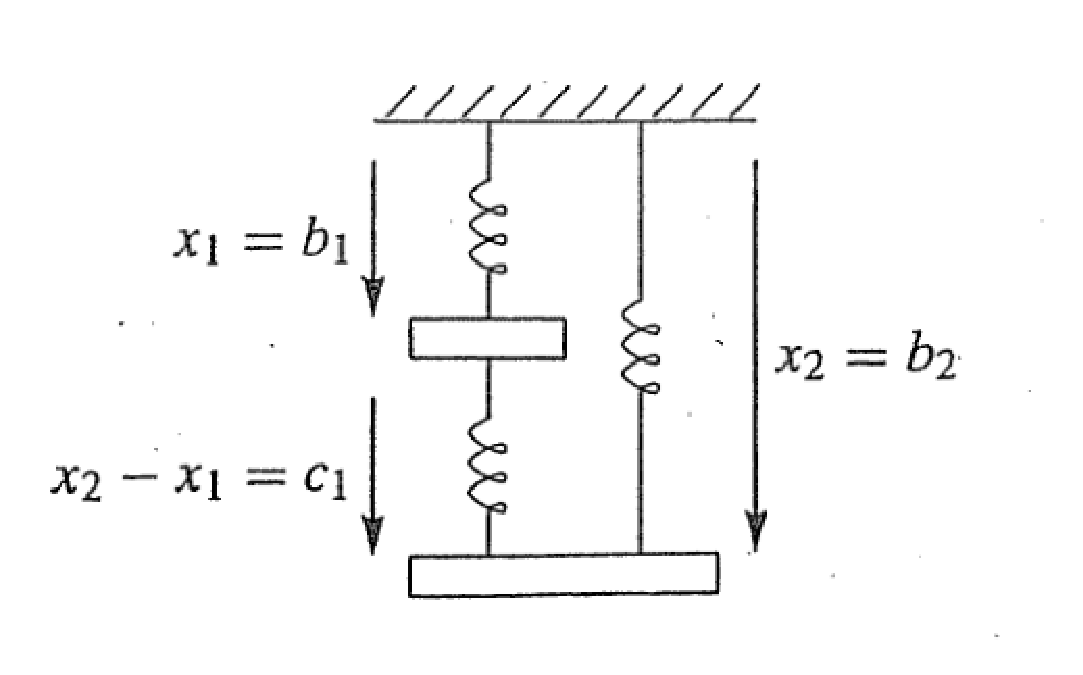
\includegraphics[width=0.7\linewidth]{TeX_files/Part02/chapter04/image/4-4}
		\caption{观测方程和状态方程的质量弹簧当量}
		\label{fig:4-4}
	\end{figure}	
	卡尔曼在每个预测/校正中增加一个弹簧 
	\begin{equation*}
	\hat{x}_{1|1}=b_1  \qquad  \hat{x}_{2|1}=b_1+c_1
	\end{equation*}
	\begin{equation*}
	\hat{x}_2=\hat{x}_{2|2}=\frac{1}{3}(b_1+2b_2+c_1)
	\end{equation*}
	
	解法 \quad  (4.30)中加权最小二乘原则仍给出$\hat{x}_1$和$\hat{x}_2$,最小化为:
	\begin{equation}
	E=\frac{1}{\sigma^2_1}(b_1-x_1)^2+\frac{1}{v^2_1}(c_1+x_1-x_2)^2+\frac{1}{\sigma^2_2}(b_2-x_2)^2
	\end{equation}
	
	加权正常方程$A^TCA=A^TCb$将有$C^{-1}=diag(\sigma^2_1,v^2_1,\sigma^2_2)$,有$C=I,\sigma_1=\sigma_2=V_1=1$:
	\begin{equation}
	\begin{bmatrix}
	\hat{x}_1  \\ \hat{x}_2
	\end{bmatrix}
	=
	\begin{bmatrix}
	b_1-c_1  \\  b_2+c_1
	\end{bmatrix}
	\end{equation}
	给出:
	\begin{equation*}
	\hat{x}_1=\frac{1}{3}(2b_1+b_2-c_1)
	\end{equation*}
	\begin{equation*}
	\hat{x}_2=\frac{1}{3}(b_1+2b_2+c_1)
	\end{equation*}
	
	最新的估计$\hat{x}_2$给了最新的观测值$b_2$一个较大的权重$\frac{2}{3}$。
	
	现在递归计算。关键的一点是$A^TCA$是三对角矩阵(在第8章中,当状态x是一个向量时,它将成为块对角矩阵)。观测方程$A_ix_i=b_i$与状态方程$x_{i+1}=F_ix_i+c_i$相连接,在三对角矩阵$A^TCA$中前向消去法总是一个递归乘法器和一个支点,然后回代是第二个递归,落后于时间。
	
	关键是事实本身,前向递归在观测方程、多达状态方程、还包括时间t=i的基础上,找到最佳估计$\hat{x}_{i|i}$,通常情况下,最终状态的估计$\hat{x}_{n|n}$是我们想要的,然后忘记回代这一步。
	
	回代这一步是调整先前的$\hat{x}_{i|i}$去解释之后的观测方程和状态方程,在时间i之后,以这种方式返回被称为“平滑”,它会使正常方程$A^TCA\hat{x}=A^TCb$产生正确的答案$\hat{x}_{i|n}$。
	
	甚至说寻找$\hat{x}_{i|i}$的前向递归是一个两步法。先前的一步$\hat{x}_{i-1|i-1}$通过时间$i-1$使用所有的信息,接下来状态方程给出一个预测,然后观测值$b_i$加上一个校正,与卡尔曼的滤波一起产生$\hat{x}_{i|i}$,预测和校正为:
	\begin{equation*}
	\hat{x}_{i|i-1}=F_{i-1}\hat{x}_{i-1|i-1}+c_i
	\end{equation*}
	\begin{equation*}
	\hat{x}_{i|i}=\hat{x}_{i|i-1}+K_i(b_i-A_i\hat{x}_{i|i-1})
	\end{equation*}
	该校正像使用增益矩阵$K_i$更新一样被写入,新数据是$c_i$和$b_i$,我们通过最小二乘,一次增加一个方程求解这个完整的系统$Ax=b$。
	
	在递归最小二乘中,有更多的一些东西需要我们计算——估计$\hat{x}_{i|i}$的可信度。协方差矩阵$P_{i|i}=(A^TCA)^{-1}_i$也是递归更新,卡尔曼滤波的每一步都增加一行(或块)到A和C中,一列(或块)到$A^T$和$C$中。预测校正步骤计算$P_{i|i-1}$和$P_{i|i}$,在$\hat{x}_{i|i-1}$和$\hat{x}_{i|i}$中的误差协方差。
	
	公平地说,卡尔曼滤波变得复杂,即使这个计划一直向前。所有的作者试图找到一个清晰的方法去推导$\hat{x}_{i|i}$和$P_{i|i}$的矩阵公式(有多种方式给数值以不同的递归)。平方根滤波用$LDL^T$或$QR$来减少当方差变得很小或很大时的数值不稳定性,我们对卡尔曼滤波的阐述将在第八章进行。
	
	最重要的一点是,协方差矩阵$P_{i|i}$像状态$x_i$具有相同的大小,这个大小与在第i步的观测数量$m_i$无关,如果我们更新最佳拟合直线,我们的矩阵保持2乘以2。
	
	例4.7 \quad (心率)在C=I(单位方差)下,递归找出P和$\hat{x}$:
	
	从$x_1=b_1$开始:\quad\quad  $A_{1|1}=[1]$  给出 $P_{1|1}=(A^TA)^{-1}_{1|1}=[I]$

	加上$x_2-x_1=c_1$:\quad $A_{2|1}=\begin{bmatrix} 1 & 0 \\ -1 & 1 \end{bmatrix}$
	和 $(A^TA)^{-1}_{2|1}=\begin{bmatrix} 1 & 1 \\ 1 & 2 \end{bmatrix}$ 给出  $P_{2|1}=2$
	
	包括$x_2=b_2$:\quad  $A_{2|2}=\begin{bmatrix} -1 & 0 \\ -1 & 1 \\ 0 & 1 \end{bmatrix}$
	和 $(A^TA)^{-1}_{2|2}=\frac{1}{3}\begin{bmatrix} 2 & 1 \\ 1 & 2 \end{bmatrix}$ 给出  $P_{2|2}=\frac{2}{3}$。
	
	第一次估计是$\hat{x}_{1|1}=b_1$(没有平滑!),使用状态方程进行接下来预测$\hat{x}_{2|1}=b_1+c_2$,使用最后的$A_{2|2}$得到校正$\frac{1}{3}(b_1+2b_2+c_1)$。
	
	那些方差$P_{2|1}=2$和$P_{2|2}=\frac{2}{3}$是$(A^TA)^{-1}_{2|1}$和$(A^TA)^{-1}_{2|2}$的最后一项,向量$x_i$引导块的支点$P^{-1}$。这里的2和$\frac{2}{3}$也被看作$b_1+c_1$和$\frac{1}{3}(b_1+2b_2+c_1)$的系数平方和。
	
	回代(平滑)在(4.32)中,调整$\hat{x}_{1|1}=b_1$成为$\hat{x}_1=\frac{1}{3}(2b_1+b_2-c_1)$。
		\section[推导卡尔曼滤波]{推导卡尔曼滤波\\Derivation of the Kalman Filter}

		\section[用于批处理的贝叶斯滤波]{用于批处理的贝叶斯滤波\\Bayes Filter for Batch Processing}

		\section[平滑]{平滑\\Smoothing}

		\section[卡尔曼方法用于稳定模型]{卡尔曼方法用于稳定模型\\Kalman Treatments of the Steady Model}

		\section[等式约束的最小二乘]{等式约束的最小二乘\\Least Squares with Equality Constraints}
		\section[固定约束的卡尔曼滤波]{固定约束的卡尔曼滤波\\Fixing Constraints in the Kalman Filter}

		\section{Quality Control}
Data processing can be performed as non-recursive (batch least-squares) or as recursive
least-squares estimation. This section contains a brief description of the models involved
and the related procedures for testing and reliability. A typical example is the situation
of possible cycle slips in the carrier phase observation. The alternative hypotheses may
consist of cycle slips in GPS carrier observations.
	\subsection{The Non-Recursive Case}
	In hypothesis testing, one usually calls the case without any model errors the null hypoth-esis $H_0$. An alternative hypothesis $H_a$ assumes there is a bias in one or several of the
	observations. Let c be a known m-vector specifying the model error, x be the n-vector of
	unknowns and s its unknown size. Then two hypotheses are defined as
	\begin{equation}
	H_0: b=Ax+e  \qquad weight\,C=\Sigma^{-1}_b
	\end{equation}
	\begin{equation}
	H_a:b=Ax+sc+e  \qquad weight\,C=\Sigma^{-1}_b.
	\end{equation}
	We assume that $m > n$.
	
	Assuming each alternative hypothesis describes the case of a single bias in an observation, the c-vectors consist of canonical unit vectors. The solution to (4.101) under the null hypothesis is given by
	\begin{equation*}
	\begin{split}
	\hat{x}&=(A^TCA)^{-1}A^TCb\\
	\Sigma_{\hat{x}}&=(A^TCA)^{-1}
	\end{split}.
	\end{equation*}
	Testing $H_0$ against $H_a$ consists of three steps:
	
	Detection\; An overall model test determines if unspecified model errors have occurred.
	
	Identification\; If a model error is detected, its potential source is identified by testing the
	original or nominal observation model (4.101) against models extended with bias	parameters, such as (4.102). 
	
	Adaptation \; After the identification of the most likely source for the model error, the observation model is adapted to eliminate the biases in the parameter vector.
	
	The projector $P=I-(A^TCA)^{-1}A^TC$ projects vectors onto the column space of
	A as demonstrated in Section 6.6. The vector of residuals is $\hat{e}=b-A\hat{x}$.
	
	In the detection step the uniformly most powerful test statistic for testing $H_0$ against
	$H_a$ is given as 
	\begin{equation}
	T=\frac{(Pb)^TCb}{m-n}=\frac{\hat{e}^TC\hat{e}{m-n}}.
	\end{equation}
	T is the overall model test statistic. Under $H_0$ and $H_a$, T is F distributed:
	\begin{equation*}
	H_0:T~F(m-n,\infty ,0) \qquad H_a:T~F(m-n,\infty ,\lambda)
	\end{equation*}	 
	The non-centrality parameter $\delta$ is defined as
	\begin{equation}
	\delta=s^2c^TCPc.
	\end{equation}
	Once reference values are chosen for the level of confidence $\alpha_0$ (the probability of rejecting $H_0$ falsely), the detection power $\gamma_0$(the probability of rejecting $H_0$  when $H_a$ is true) and the number of degrees of freedom m — n, the non-centrality parameter $\delta$ can be computed. This is the B-method of testing which was described by Willem Baarda in 1968.
	
	The B-method assumes that an error related to the non-centrality parameter $\delta_0=\delta(\alpha_0,\gamma_0,1)$ is detected with equal probability $\alpha$ by all tests. In other words from $\delta_0=\delta(\alpha_0,\gamma_0,1)=\lambda(\alpha,\gamma_0,m=n)$, with $m-n>1$, the level of confidences $\alpha$ can be computed.
	Once $\delta_0$ is known, the size of the bias that can just be detected follows from (4.104) as
	\begin{equation}
	|s|=\sqrt{\frac{\delta_0}{c^TCPc}}.
	\end{equation}
	This is the Minimal Detectable Bias (MDB). As can be seen from (4.105), the MDB depends on $\alpha_0,\gamma_0$, and the functional and stochastic model, through the design matrix A and
	the covariance matrix $\Sigma_b$ and the alternative hypothesis captured in the vector c.
	
	Remark 4.4\; We bring a detailed description of a procedure for computation of the non-centrality parameter $\delta$.
	
	First the central case (null hypothesis $H_0$): select a value for a which is the probability of an error of the first kind, that is rejecting $H_0$ falsely.
	
	MATLAB uses left tail and we need right tail, so we define $p=1-\alpha$. The number
	of degrees of freedom is f = m - n. The critical value is computed as x = chi2inv(p,f).
	This is the value where the critical region starts (rejection of $H_0$) and extends to $+\infty$.
	
	Next the non-central case (alternative hypothesis $H_a$): We know the critical value x
	and the number of degrees of freedom f, and must solve p = ncx2cdf (x,f,delta ) iteratively
	such that $\delta$ yields the known value for p.
	
	The solution from this iteration yields $\beta=p$(left tail probability of accepting $H_0$,
	while $H_0$ is true). The probability of correct decision is the “power” $\gamma=1-\beta$.
	
	For most GPS applications we set $\alpha_0=0.001,\gamma_0=0.80$ (or even higher) resulting
	in a non-centrality parameter of $\delta_0\approx 17$, see Figure 4.13. The computation is done by the M-file cct.
	
	\begin{figure}[h]
		\centering
		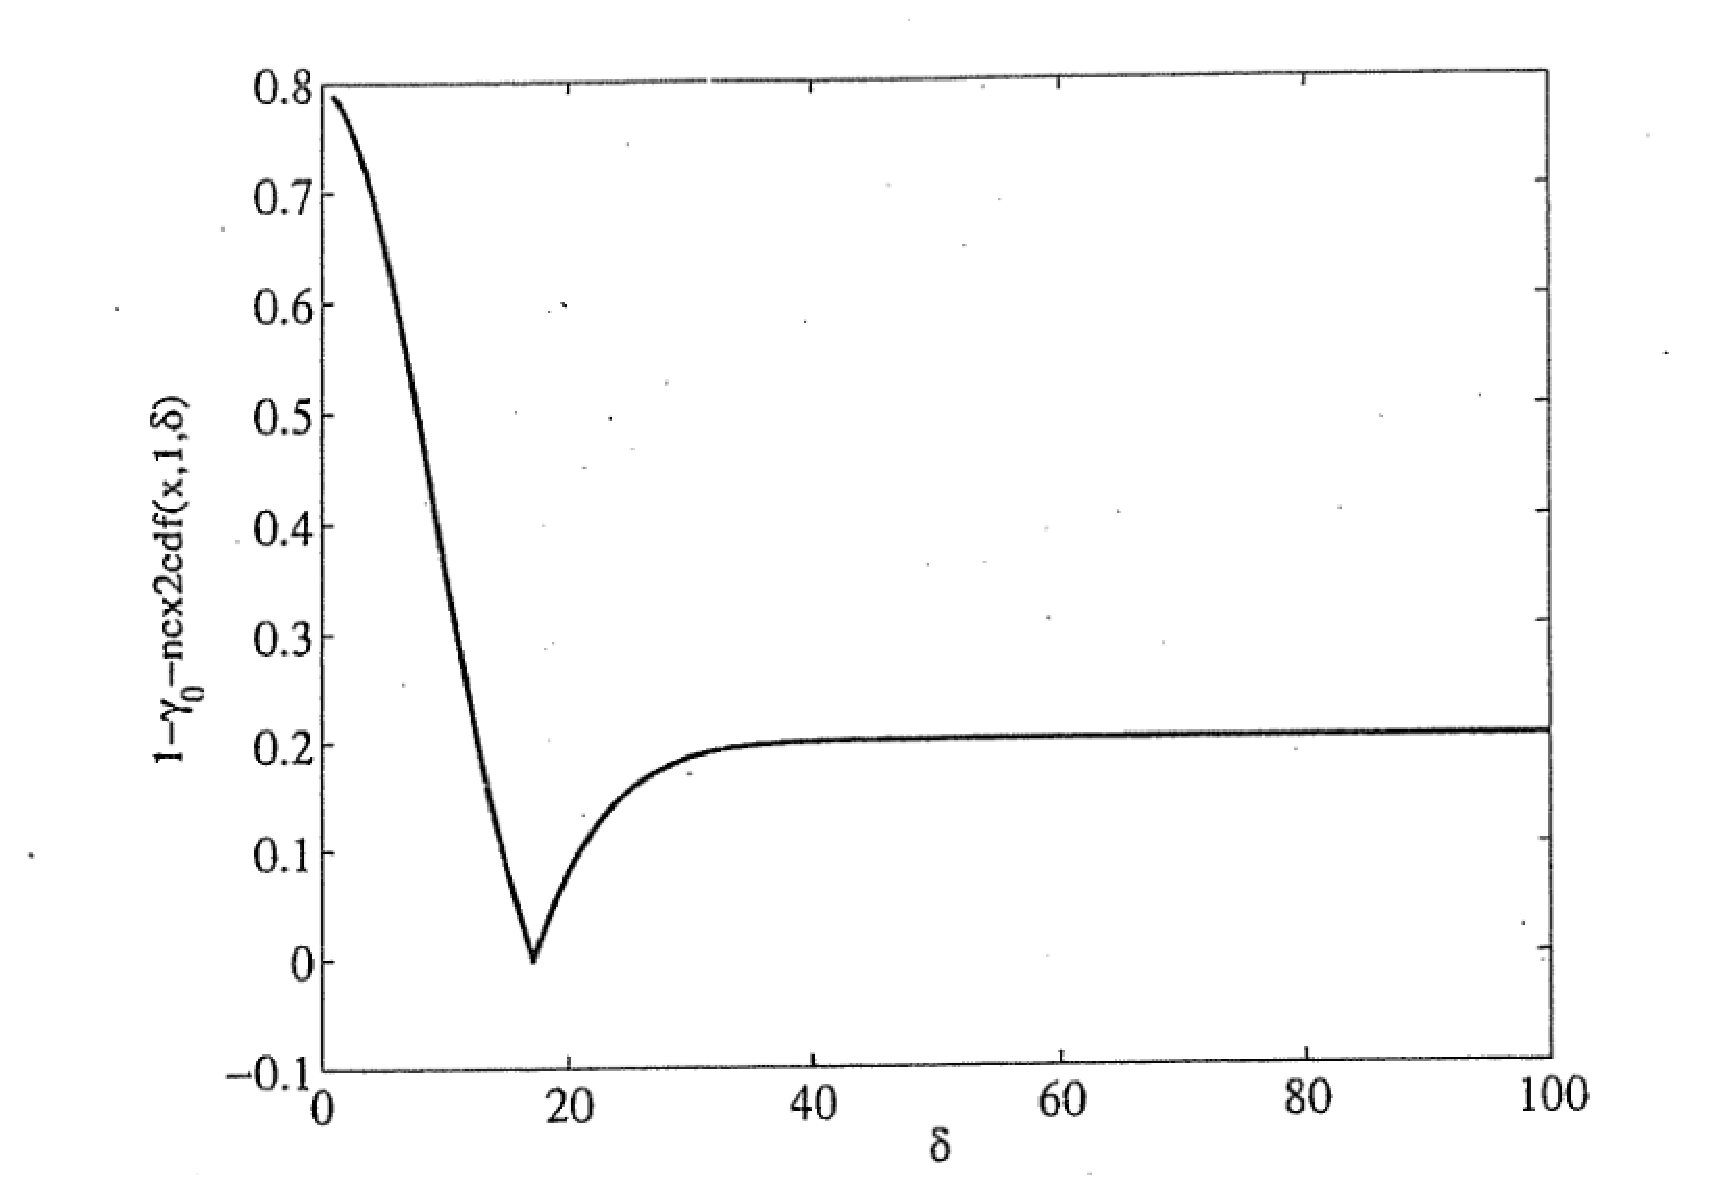
\includegraphics[width=0.7\linewidth]{TeX_files/Part02/chapter04/image/4-13}
		\caption{Figure 4.13\; The function $1-\gamma_0-ncx2cdf(x,1,\delta)$ as function of $\delta$}
		\label{fig:4-13}
	\end{figure}
	
	If the test statistic T exceeds a threshold, we say we have detected a bias s and
	the sources of the possible errors have to be found in the identification step. In practice
	this is accomplished by testing a number of alternative hypotheses, each describing one
	model error at a time, see (4.102). The uniformly most powerful test statistic for testing
	$H_0$ against $H_a$ is given as
	\begin{equation}
	t=\frac{(Pc)^TCPb}{\sqrt{(Pc)^TCPc}}=\frac{c^TCPb}{\sqrt{c^TCPc}}.
	\end{equation}
	This expression is known as a slippage test statistic. Under $H_0$ and $H_a$ the slippage test
	statistic is normally distributed
	\begin{equation*}
	\begin{split}
	 &H_0:t~N(0,1)   \\
	 &H_a:t~N(\sqrt{(Pc)^TCPc}s,1).
	\end{split}
	\end{equation*}
	The practical procedure for identifying model errors is to determine the largest slippage test statistic (in absolute value) and perform another least-squares adjustment until the
	test statistic T is accepted, or until there is no redundancy left, i.e., until m - n = 0 . Once the largest slippage test statistic t has been found, its likelihood needs to be tested. The	likelihood of the identified model error can be tested by comparing the test statistic with the critical value $N_{\alpha_0/2}(0,1)$ where $\alpha_0$ is the level of confidence. If the largest slippage test statistic t in each cycle exceeds the critical value, i.e, if
	\begin{equation*}
	|t|>N_{\alpha_0/2}(0,1)
	\end{equation*}
	then it is likely that a model error has been identified. If not, one should extend the set of alternative hypotheses to consider.
	
	For the adaptation step, several alternatives exist. One way to adapt would be to
	simply discard the bad observations (as already done, actually, in the iterated identification
	step), another to extend the vector of unknowns by one or more additional parameters.
	
	The alternative hypotheses may consist of outliers and cycle slips in GPS code and
	carrier observations, respectively. The MDB is said to describe the internal reliability of
	a system. External reliability is defined as the influence of a bias s with size equal to the
	MDB on the estimated parameters sx:
	\begin{equation*}
	sx=(A^TCA)^{-1}A^TCcs=\Sigma_{\hat{x}}A^TCcs.
	\end{equation*} 
	It should be noted that to compute internal and external reliability parameters, no actual
	data is required. They can already be computed in the design or planning phase of a survey.
	
	\subsection{The Recursive Case}
	The main difference with non-recursive or batch least squares is that for recursive least
	squares the unknown parameters are updated whenever new observations become available. Assuming the unknown parameters remain the same for an entire observation period,
	the null and alternative hypothesis for an epoch k are defined as 
	\begin{equation*}
	\begin{split}
	&H_0:b_k=A_kx   \\
	&H_a:b_k=A_kx +s_kc.
	\end{split}
	\end{equation*}
	Here we assume that a bias $s_k$ is detected and identified at the same epoch it occurred.
	in other words, we consider only local alternative hypotheses as opposed to global ones,
	which consider a number of (or even all) epochs before detecting and identifying the bias.
	Assuming a solution $\hat{x}_{k|k-1}$ with covariance matrix $P_{k|k-1}$ is available (where the subscript (k - 1) means that all epochs up to and including k - 1 were used to compute
	this solution), the recursive solution for k epochs of data under the null hypothesis is given
	as
	\begin{equation*}
	\hat{x}_{k|k}=\hat{x}_{k|k-1}+K_k(b_k-A_k\hat{x}_{k|k-1}) 
	\quad and \quad
	P_{k|k}=(I-K_kA_k)P_{k|k-1}
	\end{equation*}
	with
	\begin{equation*}
	K_k=P_{k|k-1}A^T_k(A_kP_{k|k-1}A^T_k+\Sigma_{e,k})^{-1}.
	\end{equation*}
	The vector
	\begin{equation}
	i-k=b_k-A_k\hat{x}_{k|k-1}
	\end{equation}
	is known as the innovation. Its covariance matrix is
	\begin{equation}
	\Sigma_i=A_kP_{k|k-1}A^T_k+\Sigma_{e,k}.
	\end{equation}
	Alternatively, the matrices $K_k$ and $P_{k|k}$ may be written as
	\begin{equation*}
	\begin{split}
	K_k &= P_{k|k}A^T_k\Sigma^{-1}_{e,k}\\
	P_{k|k} &=(P^{-1}_{k|k-1}+A^T_k\Sigma^{-1}_{e,k}A_k)^{-1}.
	\end{split}
	\end{equation*}
	Let $m_k$ be the number of observations at epoch k. For the detection and identification step,
	the local overall model test statistics T and local slippage test statistics t are given by
	\begin{equation*}
	\begin{split}
	&T=\frac{i^T_k\Sigma^{-1}_ii_k}{m_k}\\
	&t=\frac{c^T\Sigma^{-1}_ii_k}{\sqrt{c^T\Sigma^{-1}_ic}}
	\end{split}
	\end{equation*}
	which under $H_0$ and $H_a$ are distributed as
	\begin{equation*}
	H_0:T~F(m_k,\infty ,0) \qquad H_a:T~F(m_k,\infty ,\delta)
	\end{equation*}	
	and
	\begin{equation*}
	H_0:t~N(0,1) \qquad H_a:t~N(\sqrt{c^T\Sigma^{-1}_ic}s,1).
	\end{equation*}
	The expression for the MDB reads
	\begin{equation*}
	|s|=\sqrt{\frac{\delta_0}{c^T\Sigma^{-1}_ic}}.
	\end{equation*}
	The influence of a bias with size equal to the MDB on the estimated parameters is given as
	\begin{equation*}
	sx=sK_kc.
	\end{equation*}
	For further reading, see Teunissen \& Kleusberg (1998), Chapter 7 on “Quality Control and GPS .”
	

1\; For two independent measurements $x= b_1$ and $x= b_2$, the best $\hat{x}$ should be some
weighted average $\hat{x}=ab_1+(1-a)b_2$. When $b_1$ and $b_2$ have mean zero and
variances $\sigma^2_1$ and $\sigma^2_2$, the variance of $\hat{x}$ will be $P=a^2\sigma^2_1+(1-a)^2\sigma^2_2$. Choose the number a that minimizes P: dP/da = 0.

Show that this a gives the weighting which we have claimed to be best, using weights
$w_1=1/\sigma_1$ and $w_2=1/\sigma_2$.

2\; After N = 4 coin flips (binomial distribution) what are the five probabilities $p_0,p_1,...,p_4$ of M = 0,1,..., 4 heads? Find the mean $\bar{M}=\Sigma Mp_M$.
Show that the variance $\sigma^2=\Sigma(M-\bar{M})^2 p_M$ agrees with N/4 = 1.

3\; (a) At the center of Figure 4.3 with N = 4 and $\sigma^2=N/4 = 1$, check that the actual
height $p_2=\frac{6}{16}$ is a little below the Gaussian $p(x)=1/\sqrt{2\pi}\sigma$.

(b) The center of the Gaussian with $\sigma=\sqrt{N}/2$ has height $\sqrt{2\pi N}$. Using Stirling's approximation to N! and (N/2)!, show that the middle binomial coefficient $p_{N/2}$
approaches that height: 	
\begin{equation*}
(M=\frac{N}{2})   \quad p_{N/2}=\frac{N!}{((N/2)!)^2}\approx \frac{(N/e)^N\sqrt{2\pi N}}{((n/2e)^{N/2}\sqrt{\pi N})^2}=?
\end{equation*}	

4\; The variance $\sigma^2=\Sigma(n-\bar{n})^2p_n$  is computed around the mean $\bar{n}=\Sigma np_n$. Expand $(n-\bar{n})^2=n^2-2n\bar{n}+\bar{n}^2$ to show that this $\sigma^2$ equals $(\Sigma n^2p_n)-\bar{n}^2$.

5\; Imagine a line of masses $p_0,...,p_n$ at the points x = 0,...,n. Explain how the
mean $E\{x\}$ with probabilities $p_j$ corresponds to the center of mass. The variance $\sigma^2$
is the moment of inertia around what point?

6\; Start with r independent random variables $X_1,...,X_r$ with variances $\sigma^2_1,...,\sigma^2_r$. Show that the sum $X=X_1+...+X_r$ has variance $\sigma^2_1+...+\sigma^2_r$.

7\; One flip of a weighted coin has M = 1 (heads) with probability p and M = 0 (tails)
with probability q = 1 - p. What are the mean $\bar{M}$ and the variance $\sigma$? What are
the mean and variance for the number M of heads after N coin flips?

8\; Suppose every number is rounded down to the nearest integer. The distribution of
rounding errors e is still uniform, but on what interval of e's? What is the mean m?
What is the variance around the mean $\int(e-m)^2$ de?

9\; Suppose the random variable X has mean $\mu$ and variance $\sigma^2$.

(a) \; Show that the new variable Y = aX + b has mean $a\mu+b$.

(b) \; Show that the variance of Y is $a^2\mu^2$.

10\; Suppose X is a vector of random variables, each with mean zero, and Y = LX is
related to X by a fixed matrix L(m by n). Derive from (4.16) the “Law of Covariance
Propagation” which brings L and $L^T$ outside:
\begin{equation*}
\Sigma_Y=L\Sigma_XL^T \quad or \quad E\{YY^T\}=LE\{XX^T\}L^T.
\end{equation*}
Problems 11-14 give experience with a small-size Kalman filter

11\; In Example 4.6, extend the matrix A to 5 by 3 with $x_3-x_2=c_2$ and a new measurement
$x_3=b_3$. With unit variances in C = I, solve $A^TA\hat{x}=A^Tb$ for the best estimates $\hat{x_1},\hat{x_2},\hat{x_3}$.

Solution: With $c_1=c_2=0,\hat{x}_{3|3}=\frac{1}{8}(b_1+2b_2+5b_3)$ and $P_{3|3}=\frac{5}{8}$.

12\; In Problem 11, continue the Kalman recursion from $\hat{x_{2|2}}$ in the text to predict 
$\hat{x_{3|2}}$ and correct to $\hat{x_{3|3}}$. As in Example 4.7, find their variances $P_{3|2}$ and $P_{3|3}$ from the last entries in $(A^TA)^{-1}_{3|2}$ and $(A^TA)^{-1}$.

13\; In this Kalman example, the determinants of $A^TA$ come from the Fibonacci numbers
1,1,2,3,5,8,... as new rows are added to A. Find the three pivots of $(A^TA)_{3|3}$ as
ratios of Fibonacci numbers:
\begin{equation*}
A^TA=
\begin{bmatrix}
2&-1&0\\
-1&3&-1\\
0&-1&2
\end{bmatrix}
LDL^T  \quad with\,pivots\,in\,D.
\end{equation*} 	
14\; For $\sigma^2_1=\sigma^2_2=1$ and any $v^2_1$ in (4.31), the covariance matrix is $\Sigma=diag(1,v^2_1,1)$. Solve $A^T\Sigma^{-1}A\hat{x}=A^T\Sigma^{-1}b$. What are the limiting values of $\hat{x}_i$,as $v_1\rightarrow 0$?	
		\section[时间相关的过程噪声]{时间相关的过程噪声\\Process Noise Correlated Over Time}

		\section[离散值滤波的稳定]{离散值滤波的稳定\\Stability of Discrete Filter}

		\section[离散时间的卡尔曼滤波小项目]{离散时间的卡尔曼滤波小项目\\Mini Project on Discrete-Time Kalman Filter}
	%%----------------------------第八章结束-------------------------%%
	
%-----------------------第二部分结束---------------------------%
	
%-----------------------第三部分开始---------------------------%		
\part[定位算法]{定位算法\\Positioning Algorithms}
% \第三篇[目录标题]{正文标题}
	%%----------------------------第九章开始-------------------------%%
	\chapter[接收机伪距定位的方法]{接收机伪距定位的方法\\Receiver Position \\from One-Way Pseudoranges}
	\minitoc %小标题
	\newpage%新页
		\section[使用GPS定位]{使用GPS定位\\Positioning by GPS}
GPS对于定位和地球测量来说是一项革命性的科学技术。一方面在于其精确性,另一方面在于其快捷性和简易性。第三方面在于其廉价性。这些方面的提高导致了GPS方向的应用大量产生。我们真诚的希望我们的读者能够研发新的GPS方面的应用;GPS技术已经成熟,现在需要的是想法,并且主动将这些想法变为现实。

但是这是一本科学的书籍,不是一本宣传手册。我们专注于GPS的一个主要优势:精确度。GPS接收机自生的精确度是可以增强或减弱的。认真处理每一个流程可以提高精度,减弱是引入了显著的信号源误差。我们将使用EASY Suites描述计算的过程。

我们强烈要求重视“GPS时间”这一方面。在GPS定位中,时间是用于描述的第个四维度。这就是为什么我们需要至少四颗,而不是三颗卫星进行接收机定位的原因。这四个定位元素分别是$X$,$Y$,$Z$和$c\,dt$——光速乘以钟差$dt$。这个量$c\,dt$是距离的单位。由于普通的接收机时钟精确度仅仅只能达到秒一级,那么消除$c\,dt$的误差就不再是一个可选的,而是完全必须要处理的改进。

总而言之,GPS定位精确性的关键在于准确的卫星轨道和时间信息,在地面上,开普勒参数是通过实际观测到的轨道来计算的。这些参数上传到卫星的存储器里。卫星里携带着原子钟。它们分别播报它们自己的开普勒参数并在接收机计算。它们同时会播报低精度的其他卫星的开普勒参数。但是这些播报的参数是当前卫星轨道上最后的一部分。GPS定位的主要问题就是定位接收机。

关于GPS有一个事实我们需要注意,就是GPS测量提供的是距离而不是角度。我们通过三边测量的方法而不是三角测量的方法,这是几个世纪以来我们一直想要的,因为角度测量是绝对不方便的。当然在定位的元素$X$,$Y$,$Z$和$c\,dt$中,距离测量也是非线性的。接收机必须解决非线性的方程组。

这一章节的目的是解释GPS是如何进行定位和数学上的关系。我们将从廉价的接收机,伪距测量和有限制的精度开始。这一章使用的是小于\$1000的接收机,测量精度将达到米级。下一章我们将使用大于\$1000的接收机,高质量的接收机(或GPS网)允许使用组合码和相位测量,测量精度将达到毫米级。第十章“差分观测的方法”将处理主要的误差源并且将定位的精度等级提高到令人惊讶的程度。

同样的我们认为MATLAB软件是读者们可以自由获取的。对于这个GPS的前言,Ponsonby(1996)的讲座是特别有帮助的。
	\subsection[钟差和双曲面]{钟差和双曲面\\Clock Errors and Hyperbolas of Revolution}
	现在目标是获得一个可靠的接收机坐标。假设它们没有钟差。那么有三颗卫星到接收机的距离就可以确定一个点。每一个卫星都有一个的距离话可以在空间钟确定一个球体。首先两个球体相交可以获得一个圆。假设三个卫星不再一条直线上时,第三个球体通常和圆交于两点。一点是正确的接收机位置,另一点通常在太空中。所以三颗卫星足够定位,如果时钟是准确的并且所有的距离测量都是精确的。
	
	实际上接收机的时钟很廉价而且不精确。当钟差是$dt$时,每一个距离测量就会立即多出一项距离误差$c\,dt$。我们测量信号到达时间,其中包含的信息有发出时间。(光速大约是$c\approx300m/\mu sec.$ 当然我们使用更加精确的位数表示$c$,这对电离层误差和对流层误差有略微的不同。它们是模型误差之一。)这个不准确的测量值包含着来自未知钟差的$c\,dt$,被称为伪距。
	
	有两个卫星时我们可以获得两个伪距观测$\rho 1$和$\rho 2$。它们的差值$d^{12}=\rho 1 - \rho 2$就没有接收机误差$c\,dt$。接收机必须位于双曲线上,两个卫星分别为焦点。这个曲线图上所有的点在空间中的距离到两个卫星的差值都是$d^{12}$。
	
	第三个伪距值确定接收机在其他的双曲线上(即双曲面)。它们首先相交于曲线。第四个伪距值提供了三个独立的双曲面,它们相切在曲线上(通常是两个)。假如四个卫星不是公面的,我们再一次的获得了两个接收机可能的位置:一个准确位置、另一个在太空中,距精确值偏离了太多所以舍弃了。这个几何结构来自四个伪距观测$p^{k}$:
	\[ (X-X^{k})^{2}+(Y-Y^{k})^{2}+(Z-Z^{k})^{2}+(c dt)^{2}=(\rho ^{k})^{2} \]
	
	\subsection[参考椭球和坐标系统]{参考椭球和坐标系统\\Reference Ellipsoid and Coordinate Systems}
	接收机必须将$X$、$Y$、$Z$坐标转换至大地测量参考标准。对于GPS这个参考是WGS84。俄罗斯的GLONASS的参考系略微有所不同是PZ-90。然后接收机使用一个大地水准体模型计算地理坐标系和海拔高度。通常接收机显示纬度和经度或者在UTM投影上的北距和东距,这样可以使使用者在地图上找到坐标位置。不考虑WGS84到地图投影的修正值的话将极易导致错误。(地图投影仅仅是用来导航)实际上,地图不太可能达到厘米级的精度。尽管如此它们大概足够接近平常用户的用途了。
	\newpage
		\section[EASY Suite工具]{EASY Suite工具\\The EASY Suites}
本章和接下来的章节包含特别的教育工具。这些常见的例子你可以在大多数教科书上找到,例子中大多数的计算描述在相关的MATLAB文件中。我们将其命名为easy1$\sim$easy18的M文件。它们发布为两个部分:第一部分easy1$\sim$easy10是Borre在2003提供的。第二部分easy11$\sim$easy18发布在“Inside GNSS”期刊上。(Borre(2009a)、Borre(2009b)、Borre(2009c)、Borre (2010a)、Borre(2010b)、Borre(2010c)) 

这些文件的原始观测数据正在被维护。这个决定意味着这些文件在本书中看起来是没有归类的。为了补救这种情况我们在下一页提供了这些文件的一个表格\ref{tab:9.1}。

EASY Suite工具从2000年创建用于帮助其他人理解如何使用MATLAB 代码实现GPS定位。我们为第一部分的基础性的文件构建了一个新的专题。这个专题中包含那些能让其他人能够顺利理解的复杂代码。第二部分是其他人请求能够提供的更有价值的专业代码。
\begin{figure}[H]
	\centering
	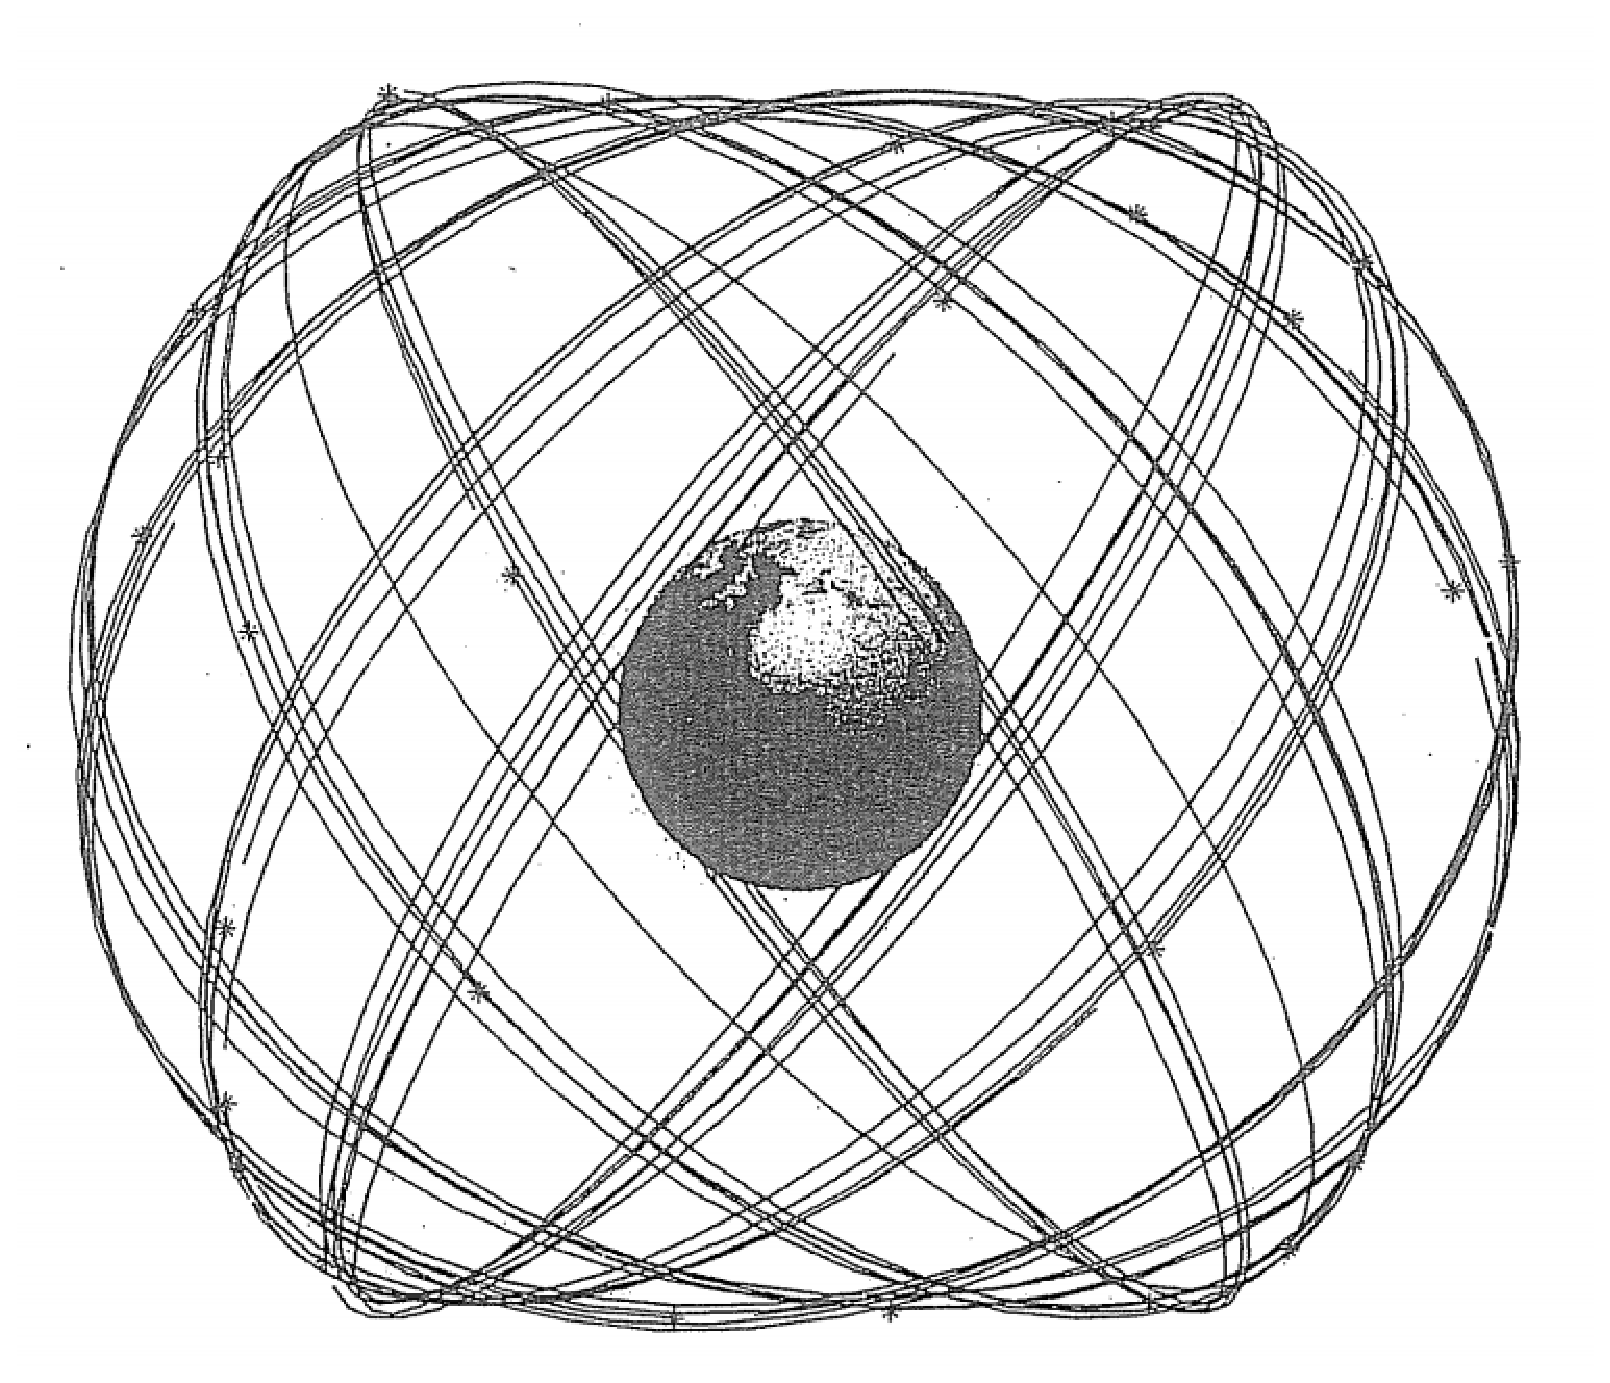
\includegraphics[width=0.4\linewidth]{TeX_files/Part03/chapter09/image/9-1}
	\caption{卫星轨道惯性坐标系——轨道穿过赤道和格林威治子午线(0°纬度、经度0°)。GPS卫星星座有6个轨道面每个上面有4个卫星。绕轨道/天15分钟完成,生产小偏移在每个轨道。}
	\label{fig:9-1}
\end{figure}
\begin{table}\label{tab:9.1}
	\caption{EASY Suites的项目列表}
	\small %设置表格字体大小
	\begin{tabularx}{\textwidth}{cXc}
		\hline  \rule[-2ex]{0pt}{5.5ex}   名称  & 					专题 						  & 页码\\ 
		\hline  \rule[-2ex]{0pt}{5.5ex}  easy1  & 时间转换:时间、UTC、GPS时间、GPS周和GPS秒  		& 第\pageref{subsec:easy1}页 \\ 
		\rule[-2ex]{0pt}{5.5ex}  easy2  & 开普勒法则,使用卫星星历计算卫星位置 			 & 第\pageref{subsec:easy2}页  \\ 
		\rule[-2ex]{0pt}{5.5ex}  easy3  & 使用伪距观测值计算接收机在ECEF系下的坐标 		 & 第\pageref{subsec:easy3}页  \\ 
		\rule[-2ex]{0pt}{5.5ex}  easy4  & 使用伪距单独计算基线					   	    & 第\pageref{subsec:easy4}页  \\ 
		\rule[-2ex]{0pt}{5.5ex}  easy5  & 使用伪距和载波计算基线,观测值使用最小二乘求解 	& 第\pageref{subsec:easy5}页\\ 
		\rule[-2ex]{0pt}{5.5ex}  easy6  & 和上面相同,但是现在用卡尔曼滤波估算基线	  	   & 第\pageref{subsec:easy6}页  \\ 
		\rule[-2ex]{0pt}{5.5ex}  easy6e & 和例5相同,但是引入带权重的观测值 			   & 第\pageref{subsec:easy6e}页 \\
		\rule[-2ex]{0pt}{5.5ex}  easy7  & 估算接收机时钟偏移量 							& 第\pageref{subsec:easy7}页\\ 
		\rule[-2ex]{0pt}{5.5ex}  easy8  & 检查周跳和接收机时钟重置 						  & 第\pageref{subsec:easy8}页   \\ 
		\rule[-2ex]{0pt}{5.5ex}  easy9  & 各种坐标下的给定基线 							& 第\pageref{subsec:easy9}页   \\ 
		\rule[-2ex]{0pt}{5.5ex}  easy10 & 估计电离层延迟对个别卫星的影响			 		& 第\pageref{subsec:easy10}页   \\ 
		\rule[-2ex]{0pt}{5.5ex}  easy11 & 卫星轨道的立体天球图和在当地局部范围的实时预报图 & 第\pageref{subsec:easy11}页   \\ 
		\rule[-2ex]{0pt}{5.5ex}  easy12 & 通过解释一个小的数值的例子来描述LAMBDA模型的细节 & 第\pageref{subsec:easy12}页   \\ 
		\rule[-2ex]{0pt}{5.5ex}  easy13 & 接收机自主完备性监测、水平防护和竖直防护等级 & 第\pageref{subsec:easy13}页   \\ 
		\rule[-2ex]{0pt}{5.5ex}  easy14 & 星基增强系统的样例,校正位置及其在斯坦福图中的呈现 & 第\pageref{subsec:easy14}页   \\ 
		\rule[-2ex]{0pt}{5.5ex}  easy15 & 对伪距单点定位、伪距基线结算和伪距载波联合观测的精度比较 & 第\pageref{subsec:easy15}页   \\ 
		\rule[-2ex]{0pt}{5.5ex}  easy16 & 筛选单向观测进行误差分析 							& 第\pageref{subsec:easy16}页   \\ 
		\rule[-2ex]{0pt}{5.5ex}  easy17 & 卫星轨道在惯性地固坐标系、地心地固坐标系下的图像 & 第\pageref{subsec:easy17}页   \\ 
		\rule[-2ex]{0pt}{5.5ex}  easy18 & 在基站计算不同的改正							 & 第\pageref{subsec:easy18}页   \\ 
		\hline 
	\end{tabularx} 
\end{table}	
原始观测数据是2001年9月4号位于奥尔堡(瑞士)的两台JPS Eurocard接收机收集的。最终生成的Rinex文件分别是site247j.01o、site24$\sim$1.01o、site247j.01n。对于其他需要长时间连续观测的特殊专题,它们所使用的文件被包含在kofi1.01o中。

上面所有提及文件的压缩包在网上都可以获取,网址是http://gps.aau.dk/~borre/esay/和http://gps.aau.dk/~borre/esay2/。
	\subsection[卫星轨道]{卫星轨道\\Orbits of the Satellites}
	卫星的轨道高度大约为3倍的地球半径。轨道接近于圆形,两个完整的轨道为一个恒星日。根据经验伪距观测值在卫星的高度角最小为$10^\circ$或大于$15^\circ$的范围时最可靠。图9.1显示了二维的早期24星的GPS星座图,在这6个轨道面上每一个都有四颗卫星。现在我们有31颗卫星。


	\label{subsec:easy17}\subsection[例子17]{例子17\\easy17}
	
	初学者对卫星轨道的样子实际上经常会有不同的想法。今天由30颗卫星组成的星座在6个不同的轨道面上,轨道面和赤道的夹角为$55^\circ$和之前的轨道面相比这个旋转了$60^\circ$.图\ref{fig:9-1}显示的情况看起来好像距离很远,因此我们叫做惯性参考框架。
	\begin{figure}
	\centering
	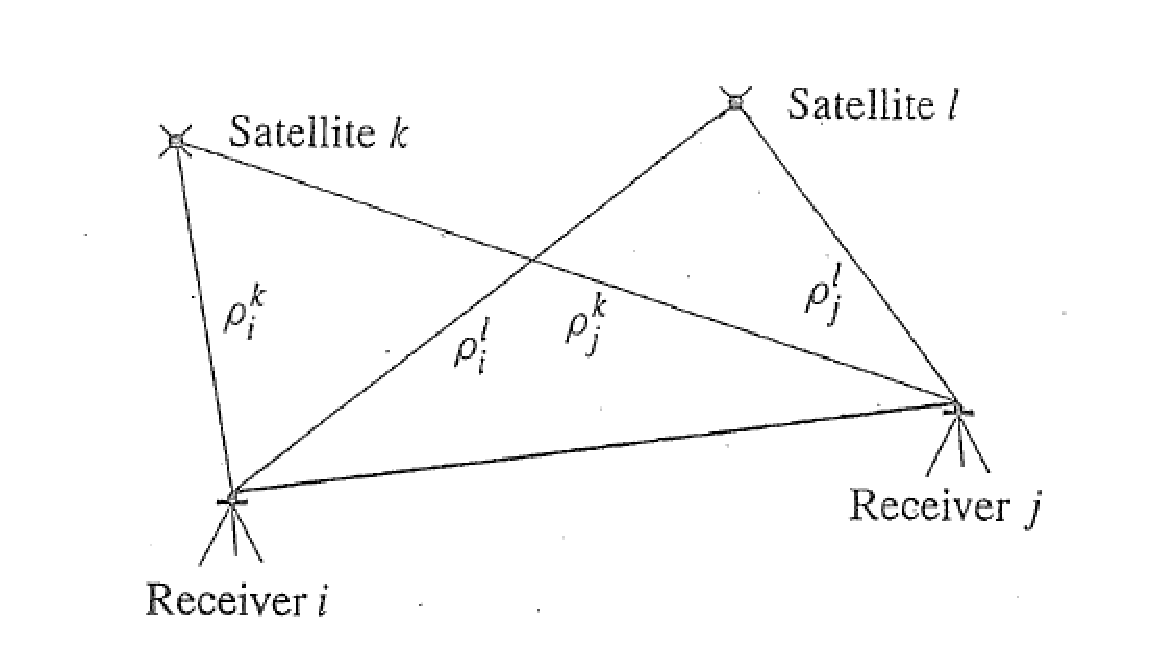
\includegraphics[width=0.4\linewidth]{TeX_files/Part03/chapter09/image/9-2}
	\caption{在ECEF框架下的卫星轨道}
	\label{fig:9-2}
	\end{figure}

	然而当这幅图像在旋转的地球平面上就显得不太清楚了。轨道到底是什么样的呢?非常奇怪。图\ref{fig:9-2}描述了这一情况。现在我们使用的是叫做地心地固坐标系(ECEF)。ECEF坐标系和旋转的地球具有固定的联系。那就是,给定一个点在一个坐标框架下的平面内是固定,除了那些可以移动的壳?(不懂)
	\begin{figure}
	\centering
	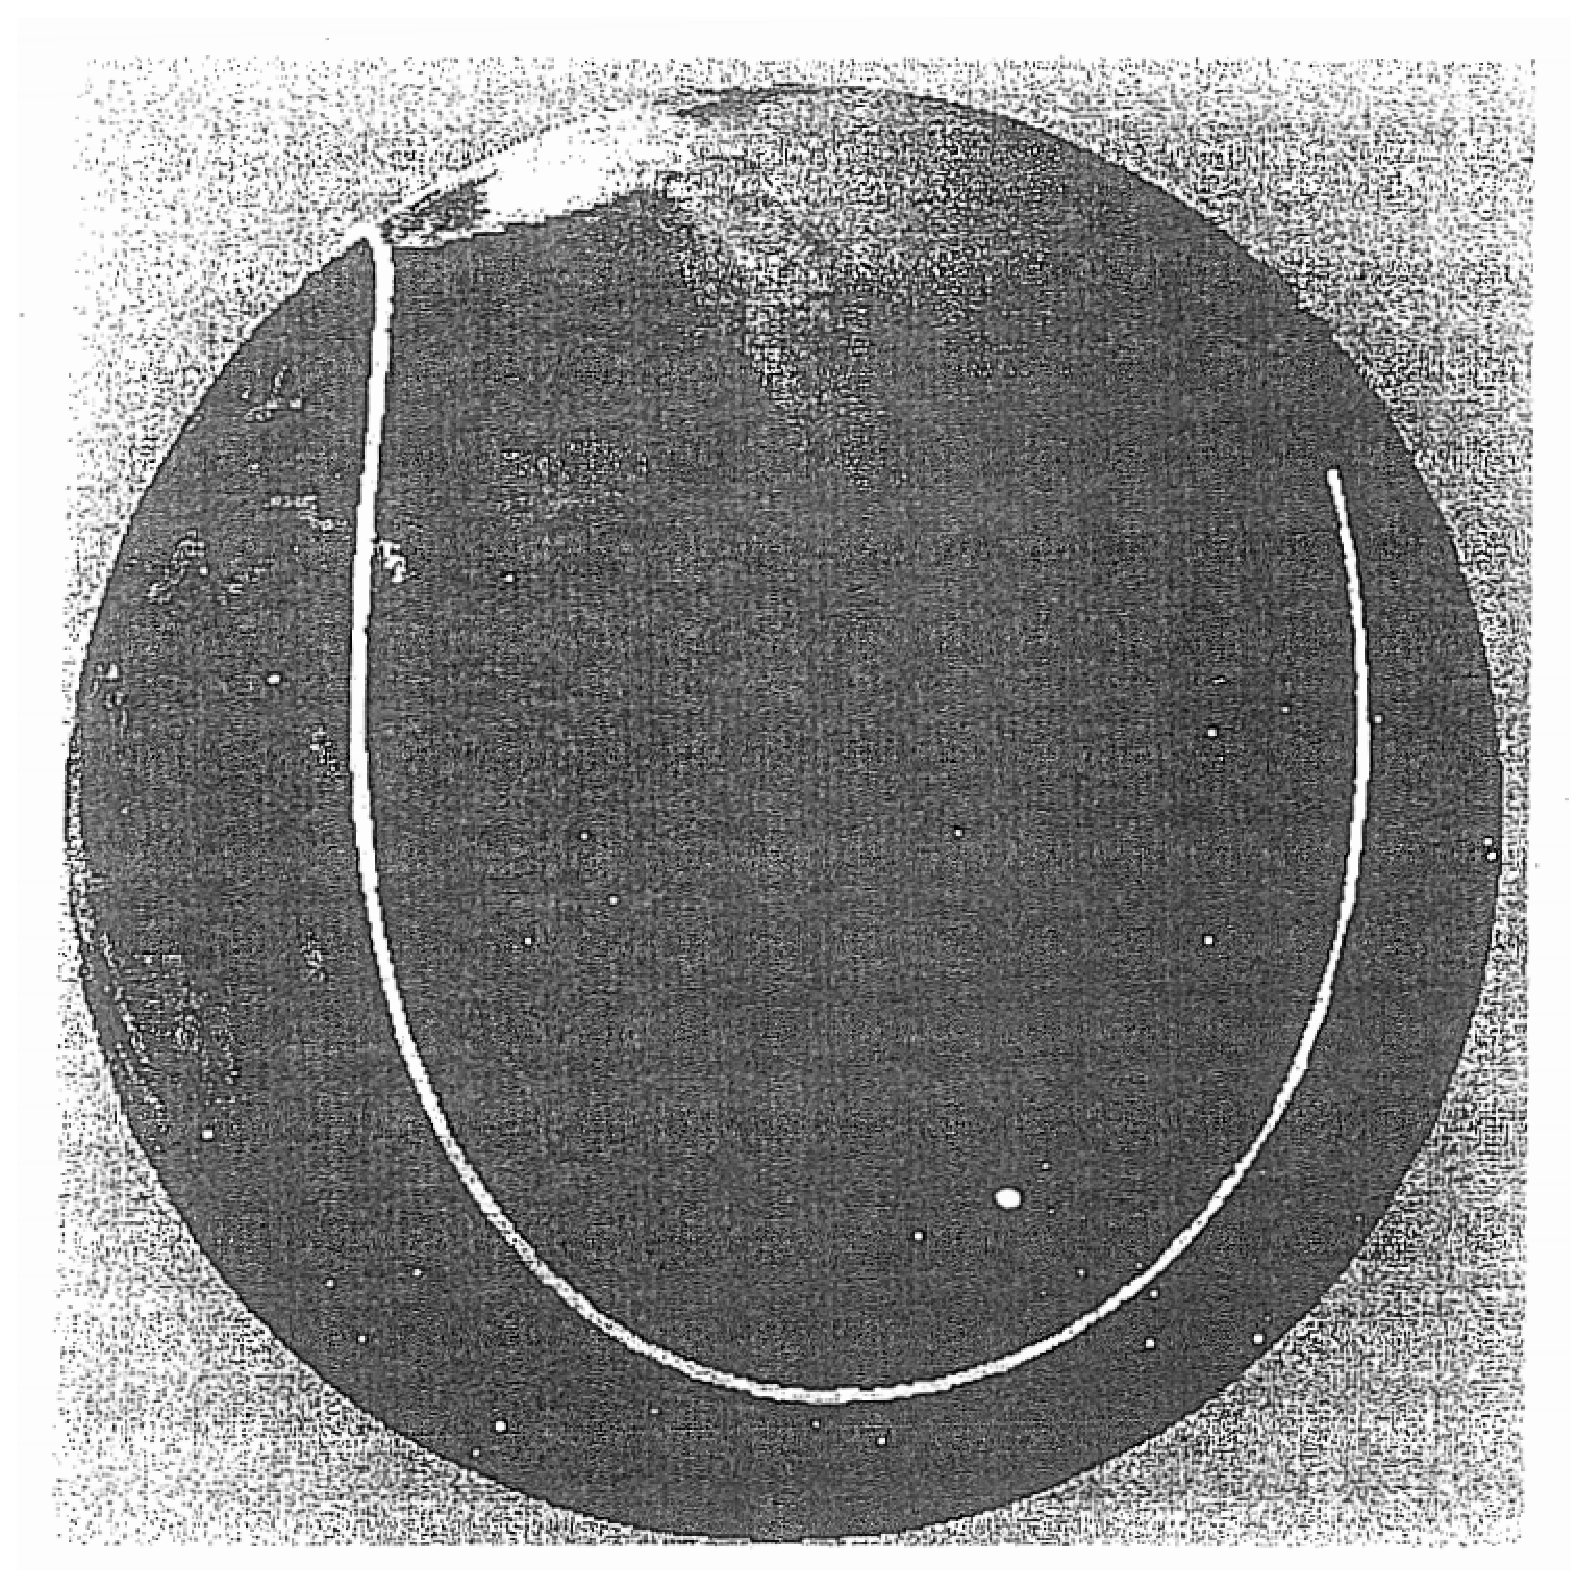
\includegraphics[width=0.4\linewidth]{TeX_files/Part03/chapter09/image/9-3}
	\caption{子卫星点选择的卫星。子卫星的曲线是由点的任意一个轨道的一部分。曲线之间的交点是地球表面和地球中心连线到卫星。}
	\label{fig:9-3}
	\end{figure}

	最后图9.3显示的曲线是子卫星在轨道上任意点的图像。这个曲线和地球中心到卫星的连线所在平面相交。子卫星的轨道在赤道两侧是对称的。这限制了向北和向南的对于轨道和赤道的夹角。
	\newpage
		\section[时间系统对于GPS的意义]{时间系统对于GPS的意义\\Time Systems Relevant for GPS}

	\subsection[狭义相对论和广义相对论]{狭义相对论和广义相对论\\Special and General Relativity}
		
	GPS定位中相对论效应是为数不多的必须要考虑的日常事件。整个系统是基于时钟的,时钟会发生偏移。
	
	所有的时钟都在地球的引力场中,所以广义相对论是很重要的。时钟信号的标称频率为10.23 MHz。实际上,由于相对论效应的影响,卫星钟准确的频率是10.22999999943 MHz 这样就和用户在地球上的10.23 MHz的频率一致了。
	
	由于卫星时钟相对与接收机时钟是运动的,所以在狭义相对论的情况下时间膨胀了。并且地球一直在旋转,光线跟随着螺旋的路径。我们不能完全同步时钟。
	
	萨尼亚克效应的旋转也是迷人的。它破坏了爱因斯坦的同步,这取决于一个常数的光速。这种恒定性局限于惯性系(无相对加速度)。地球的旋转意味着时钟A可以同步时钟B,时钟B可以同步时钟C,但时钟C不同步时钟A。所以我们需要一个世界时,会以不同的速度同步当地时间。这种协调世界时保持在科罗拉多斯普林斯的GPS控制中心。
	
	\subsection[GPS时间和跳秒]{GPS时间和跳秒\\GPS Time and Leap seconds}
	GPS的基本时间单位是国际单位制(SI)的秒。国际单位制的秒在1967年的第13届的国际计量大会上被定义为“铯原子$Cs^133$基态的两个超精细能级间跃迁辐射振荡9192631170周所持续的时间”。国际单位制的天被定义为84400SI秒,一个儒略世纪是36525(SI)天。
	
	为了弥补真太阳时不均匀的缺陷,人们定义了一个假太阳,其运动轨道位于赤道平面,并且它在赤道上的运动角速度时恒定的。平太阳的时角叫做世界时(UT)。

	儒略日JD日期的表达是一段固定的时间和在基本历元后的部分时间(???)。儒略日的起点为公元前4713年1月1日 $12^h$ 世界时。儒略日时间表示日期是连续计数的,
	
	当前时间用JD表示是一个数值比较大的数,所以使用简化儒略日MJD来代替。
	$$MJD = JD-2 400 000.5.$$
	因此J2000.0(公元2000年) = MJD 51544.5。MJD是以1858年11月17日平子夜作为起点。
	\begin{table}
		\centering
		\caption{UTC和GPST之间的调整日期和跳秒数}
		\label{tab:9.2}
		\begin{tabular}{cc}
			\hline 跳秒数 & 调整日期 \\ 
			\hline  
			1 & 1982-06-30 \\ 
			2 & 1983-06-30 \\ 
			3 & 1985-06-30 \\ 
			4 & 1987-12-31 \\ 
			5 & 1989-12-31 \\ 
			6 & 1990-12-31 \\ 
			7 & 1992-06-30 \\ 
			8 & 1993-06-30 \\ 
			9 & 1994-06-30 \\ 
			10 & 1995-12-31 \\ 
			11 & 1997-06-30 \\ 
			12 & 1998-12-31 \\ 
			13 & 1999-12-31 \\ 
			14 & 2005-12-31 \\ 
			15 & 2008-12-31 \\ 
			\hline 
		\end{tabular} 
	\end{table}
	
	为了在世界范围内保持时间和完整的描述闰秒。国际原子时间尺度(TAI)不与太阳时保持同步,由于地球的自转速度是每年放缓近1s。实现平均太阳时称为世界时(UT1)。协调世界时(UTC)与国际原子时(TAI)由一个整秒数的偏移量定期更新,以保持UTC接近UT1。
	
	跳秒是由IERS(国际地球自转服务)提出的,所以协调世界时(UTC)与世界时(UT1)的时刻差不能大于0.9s。(国际地球自转服务也负责维护的连续性与早期光学仪器采集的数据)DUT1是UT1-UTC的差值,播出的时间信号的精度为$\pm$0.1 s
	
	时间信号由GPS卫星广播,而GPS卫星的时间与GPS主控制站(位于科罗拉多州)的原子钟时间同步。全球定位系统时间GPST的起始时刻为1980年1月6日$0^h$,起始时刻与UTC对齐,但并不增加UTC的闰秒。因此,有一个整秒数的偏移抵消GPST和TAI之间19s的差值。
	$$GPST + 19 s = TAI.$$
	表格\ref{tab:9.2}显示了从1980年1月6日到2011年的所有的15个跳秒。
	$$GPST = UTC + 15 s.$$
	
	随着GPST,从一开始介绍了GPS周数。自1980年1月6日,每周都有自己的编号。这本书写在第1625周。在一周中有了周积秒(sow)的概念。这个数字计数是从周六的午夜开始的,周日是GPS一周的开始。
	
	另外为了方便,每周的每一天有一个数字编号:周日是1,周一是2,周二是3,周三是4,周四是5,周五是6,周六是7。
	
	专业的GPS软件使用周积日(dow)有数值的原因。周积秒(sow)就像这么$7 \times 24 \times 60 \times 60 = 604 800 s$大。为了跟踪一个点的位置(mm级),我们必须保证时间在0.01ns的精度水平。使用周积秒(sow)和12位小数超出了大多数计算机的计算能力。所以你可能将一周内真正的秒数分割成一个整数部分和小数部分或者计算时间的GPS周数,周积日和日积秒。
	
	M文件 $gps\_time$ 用于计算GPS时间 (GPS周(w)和周积秒(sow)):
	\begin{lstlisting} 
	t = julday(2011,3,2,10); % year, month, day, hour
	[w,sow] = gps_time(t)
	w = 1625
	sow = 295200
	\end{lstlisting}
	为了避免在一周的开始和结束时发生低于或高于限制的错误我们使用M文件$check\_t$。
	\subsection[例子1]{例子1\\easy1}\label{subsec:easy1}
	几乎所有GPS的处理都开始自时间问题,\ref{subsec:easy1}展示了如何将一个给出年,月,日,小时,分钟,秒和儒略日的历元时间转化为,GPS周和周积秒(sow)。
	
	下面是sate247j的RINEX格式的观测文件的样本:
	
	\begin{figure}
		\centering
		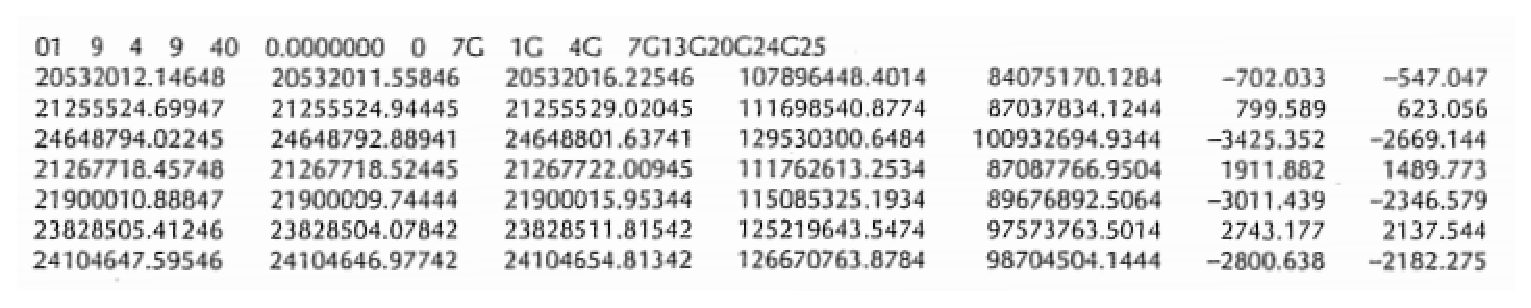
\includegraphics[width=1.0\linewidth]{TeX_files/Part03/chapter09/image/9-site247j}
	\end{figure}
	
	这个数据块的第一行告诉历元时间和有哪些观测到的伪随机噪声卫星。我们解释一下时间是2001年4月9日在9小时40分0秒。随后的0表示接收机处于静态模式;接下来我们读到接收机对7个GPS卫星1、4、7、13、20、24、25进行跟踪。
	
	下面的七行包含七个卫星的伪距和载波观测值有:L1上C/A码所测定的伪距,L1和L2上的P码所测定的伪距,L1和L2上的相位观测值,L1和L2上的多普勒频率。
	
	\subsection[估计接收机时钟偏移量]{估计接收机时钟偏移量\\Estimation of Receiver Clock Offset???}
	现在我们开始使用数据。第一步是估计时钟偏移量$c\,dt_t$。在GPS测量中,观测码$b_t$(伪距)通常被用来估计一个单点的坐标和接收机时钟偏移的顺序(随时间变化)。假设历元时间t提供线性观测值$b_t$:
	
	\begin{equation}\label{eq:9.1}
	A_t 
	\begin{bmatrix}
	x \\	y \\	z
	\end{bmatrix}
	+e_tcdt_t=b_t-\epsilon _t,\qquad t = 1,2,\ldots ,n.
	\end{equation}
	矩阵$A_t$包含t时刻的伪距观测值对坐标的偏导数。后文中式\ref{eq:9.22}。添加每个伪距观测的钟差,$e_t = (1, 1,\ldots ,1 )^T$当该历元有m个卫星时其中便有m项。
	我们收集n个历元的观测值统一成为一个的最小二乘问题
	
	\begin{equation}\label{eq:9.2}
	\begin{bmatrix}
	A_1 \\	A_2 \\	\vdots \\	A_n \\
	\end{bmatrix}
	\begin{bmatrix}
	x \\	y \\	z 
	\end{bmatrix}
	+		
	\begin{bmatrix}
	e_1 & & & \\
	& e_2 & & \\	
	& & \ddots & \\	
	& & & e_n  
	\end{bmatrix}
	\begin{bmatrix}
	c\,dt_1 \\	
	c\,dt_2 \\	
	\vdots \\	
	c\,dt_n
	\end{bmatrix}
	=\begin{bmatrix}
	b_1 \\ b_2 \\ \vdots \\ b_n
	\end{bmatrix}
	-
	\epsilon
	\end{equation}
	\begin{figure}
		\centering
		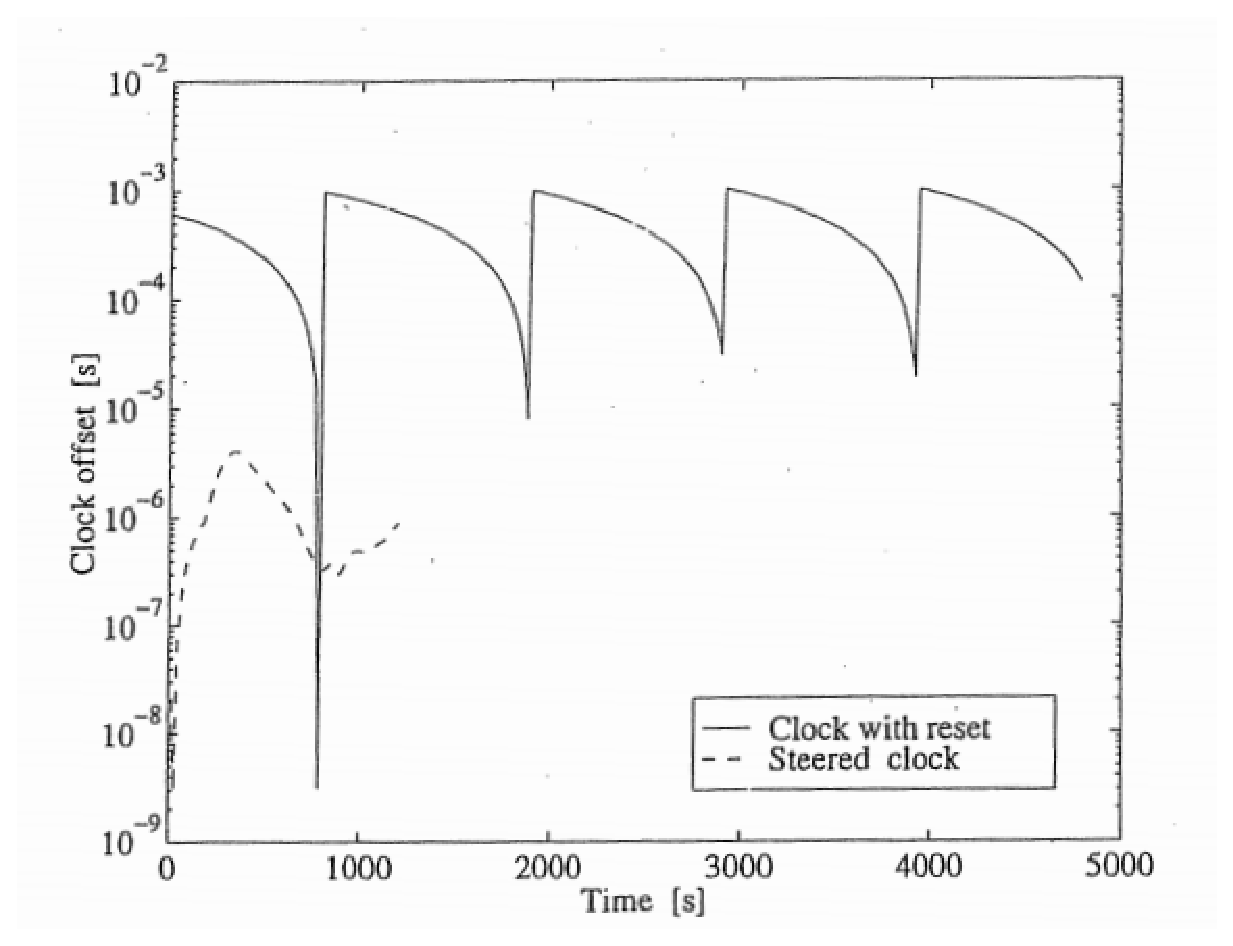
\includegraphics[width=0.7\linewidth]{TeX_files/Part03/chapter09/image/9-4}
		\caption{不同类型接收机的时钟偏移量。时钟重置时间为1ms。}
		\label{fig:9-4}
	\end{figure}
	
	正规方程组\ref{eq:9.2}通过最小二乘方法获得最优的$x,y,z,c\,dt_t$解。
	
	\begin{equation}\label{eq:9.3}
	\begin{bmatrix}
	e^T_1e_1 & & & & e^T_1A_1 \\
	& e^T_2e_2 & & & e^T_2A_2 \\
	& & \ddots   & & \vdots	  \\
	& & & e^T_ne_n & e^T_nA_n \\
	A^T_1e_1 & A^T_2e_2 & \ldots & A^T_ne_n & \Sigma ^n_{t=1}A^T_tA_t
	\end{bmatrix}
	\begin{bmatrix}
	c\,dt_1 \\
	c\,dt_2 \\
	\vdots
	c\,dt_n \\
	x \\
	y \\
	z 
	\end{bmatrix}
	=
	\begin{bmatrix}
	e^T_1b_1 \\
	e^T_2b_2 \\
	\vdots	 \\
	e^T_nb_n \\
	\Sigma ^n_{t=1}A^T_tb_t
	\end{bmatrix}
	\end{equation}
	
	使用普通高斯消元法从n个方程中消去n倍的最后一行。我们写下$E_t$矩阵$e_t(e^T_te_t)^{-1}e^T_t$ 。修正(x,y,z)坐标到初步位置(x°,y°,z°)是由矩阵右下角出现的项来消除的。根据式\ref{eq:6.46}。
	$$x=\begin{bmatrix}
	x \\ y \\ z
	\end{bmatrix}=\left( \sum^n_{t=1}(A^T_tA_t-A^T_tE_tA_t)\right)^{-1}\sum^n_{t=1}(A^T_tb_t-A^T_tE_tb_t) $$
	估计接收机时钟偏移量 $c\,dt_t$是通过回代法解决,$i=n,\ldots,1$:
	\begin{equation}
	c\,dt_t=(e_tb_t-e_tA_tx)/(e_te_t^T).
	\end{equation}
	
	估计模型清楚地显示为什么没有必要为所有历元的静态观测收集四个观测值。但需要足够数量的观测值来保持\ref{eq:9.3}是可逆的。如果只有一个观测值是可以在一个特定的历元估计接收机时钟偏移,但不能估计位置。
	\begin{figure}
		\centering
		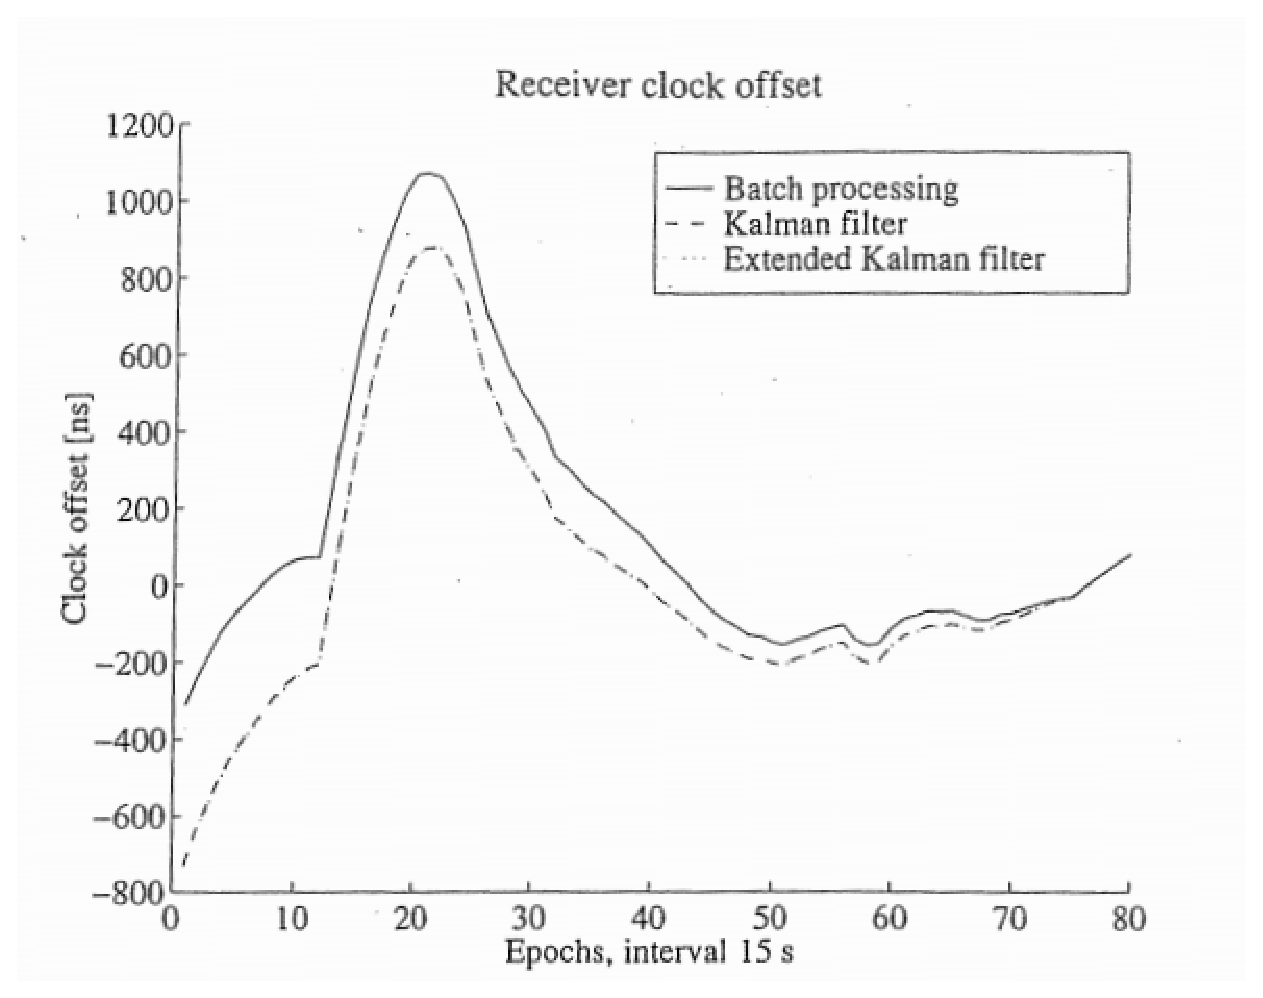
\includegraphics[width=0.7\linewidth]{TeX_files/Part03/chapter09/image/9-5}
		\caption{接收机时钟偏移计算的批处理和卡尔曼滤波。普通和扩展卡尔曼滤波的线性方程}
		\label{fig:9-5}
	\end{figure}
	
	我们建议使用描述程序,一些制造商引入不连续的时钟时间变化以保证误差在规定的补偿要求内。某些接收机时钟在复位时抵消1毫秒。图\ref{fig:9-4}展示了这种跳跃方式抵消钟差的接收机类型,以及这种类型的接收机如何操纵时钟。
	
	图\ref{fig:9-5}显示了接收机时钟偏移量与不断修正以抵消的操纵方式。图像是由M文件recclock提供。代码迭代三次得到正确的接收机位置——时钟估计是线性的!
	
	\subsection[例子7]{例子7\\easy7}\label{subsec:easy7}
	伪距这个词的“伪”部分暗指接收机时钟偏移dt。常常dt是一个不太关心的参数。然而在某些情况下需要知道dt。我们应用该算法(9.4)来获取dt。
	
	实际数据产生$dt\approx0.38 ms$ 如图\ref{fig:9-6}所示。可以看到接收机时钟的速率是在很短的时间内相当稳定。

		\section[定位卫星]{定位卫星\\Satellite Position}
		本节以地球为中心在地心地固坐标系(ECEF)$X,Y,Z$中,通过开普勒轨道参数描述卫星的空间位置。选择开普勒参数的原因是,他们随着时间变化小。之后的五页研究这些轨道参数 $a,e,\omega,\Omega ,i,$ 和$\mu$,如图\ref{fig:9-7}。这是不可避免的技术;许多读者认为可以通过ECEF找到坐标,并继续。
	\begin{figure}
		\centering
		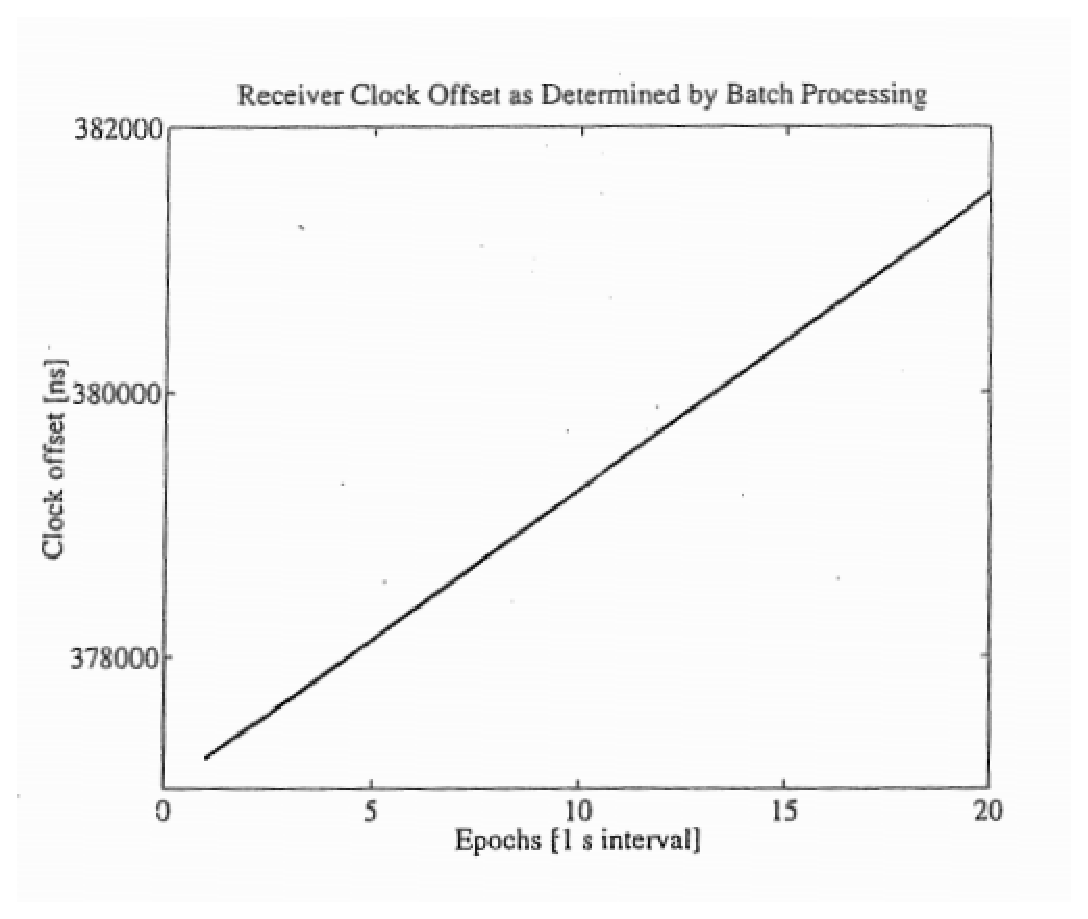
\includegraphics[width=0.7\linewidth]{TeX_files/Part03/chapter09/image/9-6}
		\caption{接收机时钟偏移量 $dt$}
		\label{fig:9-6}
	\end{figure}
	
	X轴指向赤道和格林威治子午线之间的交点。Z轴伴随着地球的自转轴。Y轴的指向正交于这两个方向,形成一个右手坐标系。
	
	轨道平面相交赤道平面交线。交线有两个点与赤道相交。卫星从南到北移动的经过的点称为升交点K。赤道平面和轨道平面之间的夹角称为轨道倾角i。地球中心C和X轴升交点K之间的夹角叫做$\Omega$;这是赤经。轨道上位置最接近地球中心的点(椭圆轨道的焦点)称为近地点。地球中心C、升交点K和近地点P之间的角叫做近地点角距$\omega$;这是从Z轴逆时针增加的方向观察的。
	\begin{figure}
		\centering
		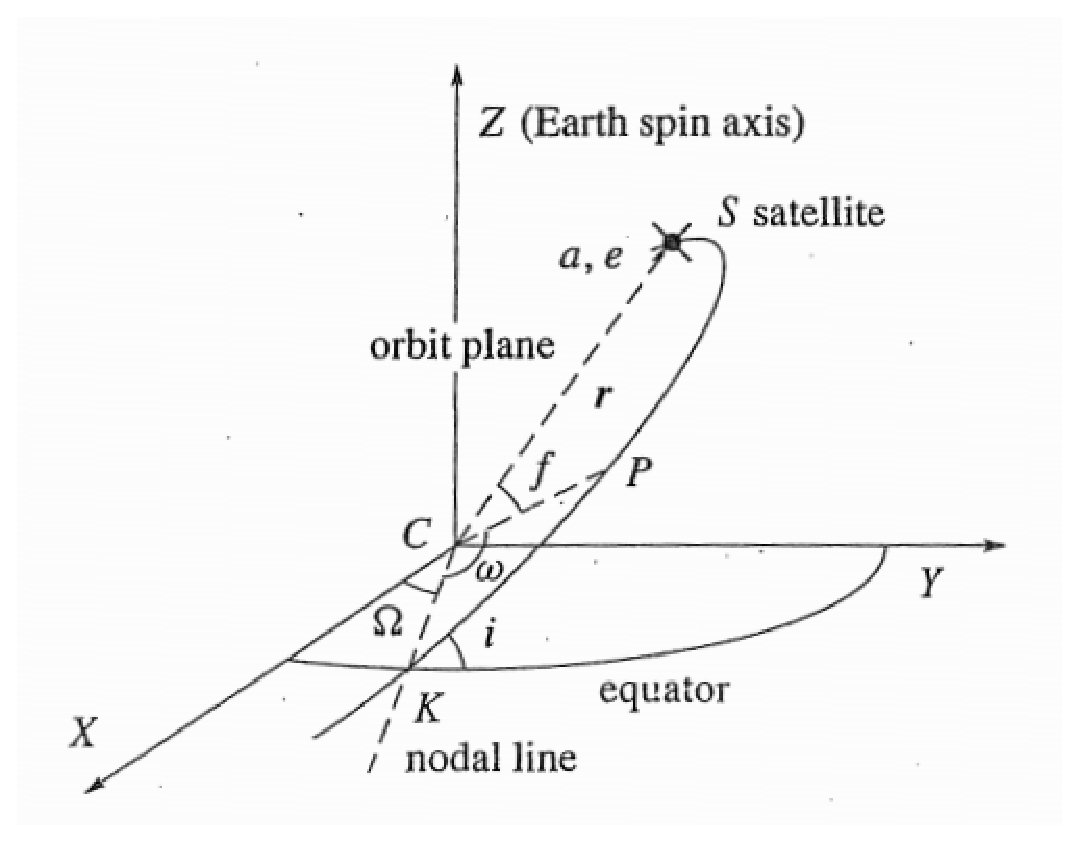
\includegraphics[width=0.7\linewidth]{TeX_files/Part03/chapter09/image/9-7}
		\caption{开普勒轨道参数:长半径 $a$,偏心率 $e$,轨道倾角 $i$,升交点$K$的赤经$\Omega$,近地点角距 $\omega$,和真近点角$f$. 近地点用$P$表示.。地球中心用$C$表示。}
		\label{fig:9-7}
	\end{figure}
	
	图\ref{fig:9-8}显示了轨道面在以地球为中心的坐标系平面中。$\xi$轴指向近地点$\eta$轴指向降交点。$\xi$轴和轨道面正交。从图\ref{fig:9-8}我们可以获得偏近点角$E$和真近点角$f$。我们可以获得:
	\begin{figure}
		\centering
		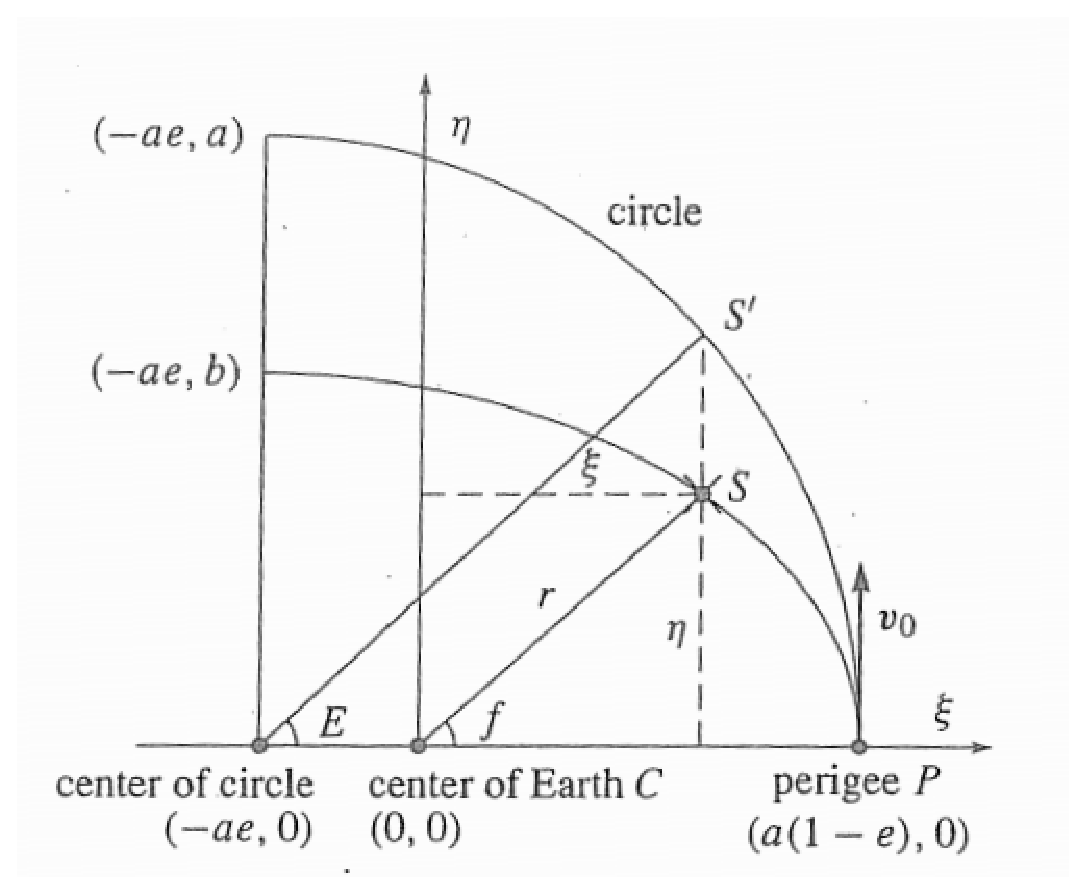
\includegraphics[width=0.7\linewidth]{TeX_files/Part03/chapter09/image/9-8}
		\caption{椭圆轨道在$(\xi,\eta)$坐标系中。真近点角$f$位于地球中心$C$.}
		\label{fig:9-8}
	\end{figure}
	$$\xi = r \cos f = a \cos E - ae = a (\cos E -e). $$
	$$\eta = r \sin f = \frac{b}{a} \sin E = b \sin E = a\sqrt{1-e^2}\sin E.$$
	
	因此,卫星坐标向量$r$在以地球中心$C$表示时是:
	\begin{equation}\label{eq:9.5}
	r=\begin{bmatrix}
	\xi \\ \eta \\ \zeta
	\end{bmatrix}
	=\begin{bmatrix}
	a(\cos E -e) \\
	a\sqrt{1-e^2}\sin E \\
	0
	\end{bmatrix}.
	\end{equation}
	
	通过三角函数变换可以得到下式:
	\begin{equation}\label{eq:9.6}
	\lVert r \lVert = a(1-e\cos E).
	\end{equation}
	一般角E随时间t变化,长半轴a和偏心率e几乎是恒定的。(对于e有长时间运行和短周期扰动,对于a只有短周期扰动。)$\lVert r \lVert$是卫星s到地球中心$C=(0,0,0)$的几何距离
	
	为了供以后参考我们引入平均值n即意味着角卫星运动速度。如果卫星的一个旋转周期是T,并且$GM = 3.986005 • 10^14 m^3/s^2$ 我们就有:	
	\begin{equation}\label{eq:9.7}
	n = \dfrac{2\pi}{T} = \sqrt{\dfrac{GM}{a^3}}.
	\end{equation}
	
	现在,是时候来定义平近点角$\mu$。这个非几何量定义为近地点和一个虚构的卫星之间的角度在圆形轨道卫星同样的焦距和同一周期的情况,但以一个恒定的速度移动。恒速是指卫星的运动。真实的和虚构的卫星穿越近地点和远地点的阶段,对于虚构的卫星,卫星的平均异常是真正的异常。是在t时刻的异常。(???)
	$$\mu = n(t-t_0)$$
	
	$t_0$是穿过近地点的时间。注意$\mu$ 是一个关于时间的线性函数的时间对于圆形轨道我们有$\mu = f + \omega$,参考Misra $\&$ Enge (2006).
	
	著名的开普勒方程关系两个角度,异常值$\mu$和偏近点角E:
	\begin{equation}\label{eq:9.8}
	E = \mu + e\sin E
	\end{equation}
	
	从式\ref{eq:9.5}中我们可获得
	\begin{equation}\label{eq:9.9}
	f = \arctan \frac{\eta}{\xi} = \arctan \dfrac{\sqrt{1-e^2}\sin E}{\cos E-e}
	\end{equation}
	这样我们获得了真近点角f,偏近点角E,平近点角$\mu$。这些关系式是计算卫星位置的基础。
	
	描述开普勒轨道六参数可以构成的一个轨道,所以他们在表\ref{tab:9.3}重复显示。
	
	重要的是要意识到轨道平面在地心坐标系X,Y,Z中仍相当稳定。换句话说:从太空轨道平面仍然和赤道保持固定关系。格林威治子午线平面绕地球自转轴的运动按照格林尼治恒星时(GAST),速度大约是24小时/天。GPS卫星每天绕行两周,它的轨道速度为3.87公里/秒。	
	
	卫星K的轨道平面在笛卡尔坐标系下的图像如图\ref{fig:9-7},我们可以获得
	$$\begin{bmatrix}
	r^k_j\cos f^k_j \\
	r^k_j\sin f^k_j \\
	0
	\end{bmatrix},$$
	
	$r^k_j = \lVert r(t_j)\lVert$由式\ref{eq:9.6}获得,其中$a,e,$和$E$是在时刻$t = t_j$时的值。
	
	这个向量旋转到X,Y,Z坐标系统的三维旋转矩阵对于图\ref{fig:9-7}为:
	$$R_3(-\Omega^k_j)R_1(-i^k_j)R_3(-\omega ^k_j).$$
	
	矩阵绕XY平面的旋转角为$\varphi$,同时Z方向不变。
	\begin{equation}\label{eq:9.10}
	R_3(\varphi) = 
	\begin{bmatrix}
	\cos \varphi & \sin \varphi & 0 \\
	-\sin \varphi & \cos \varphi & 0 \\
	0 & 0 & 1
	\end{bmatrix}
	\end{equation}
	
	同理$R_1(\varphi)$给出了关于X轴的旋转:
	
	\begin{table}
		\caption{卫星轨道的开普勒参数}
		\label{tab:9.3}
		\begin{tabularx}{\textwidth}{lX}
			\hline $a$ 长半轴 &  \multirow{2}*{轨道大小和形状参数} \\
			$e$ 偏心率 &  \\ 
			\hline $\omega$ 近地点角距 & \multirow{3}{150pt}{轨道平面的参数} \\ 
			$\Omega$ 升交点赤经 &  \\ 
			$i$ 倾角 &  \\ 
			\hline $\mu$ 平近点角 & 在平面的位置 \\ 
			\hline 
		\end{tabularx} 
	\end{table}
	
	\begin{equation}\label{eq:9.11}
	R_1(\varphi) = 
	\begin{bmatrix}
	1 & 0 & 0 \\
	0 & \cos \varphi & \sin \varphi \\
	0 & -\sin \varphi & \cos \varphi \\
	\end{bmatrix}
	\end{equation}
	
	卫星K在$t_j$时刻的地心坐标系下的坐标是:
	\begin{equation}\label{eq:9.12}
	\begin{bmatrix}
	X^k(t_j) \\ Y^k(t_j) \\ Z^k(t_j) 
	\end{bmatrix}
	=
	R_3(-\Omega ^k_j)R_1(-i^k_j)R_3(-\omega ^k_j)
	\begin{bmatrix}
	r^k_j \cos f^k_j \\
	r^k_j \sin f^k_j \\
	0
	\end{bmatrix}
	\end{equation}
	
	然而,GPS卫星不遵循了正常的轨道理论。我们必须使用与时间有关的更精确的轨道值:随时间变化的开普勒参数或与其等价的参数。在下文中,通过广播星历可以获得。我们把这些值插入在一个步骤后面,最后我们得到了一组变量式\ref{eq:9.12}。
	
	\begin{figure}
		\centering
		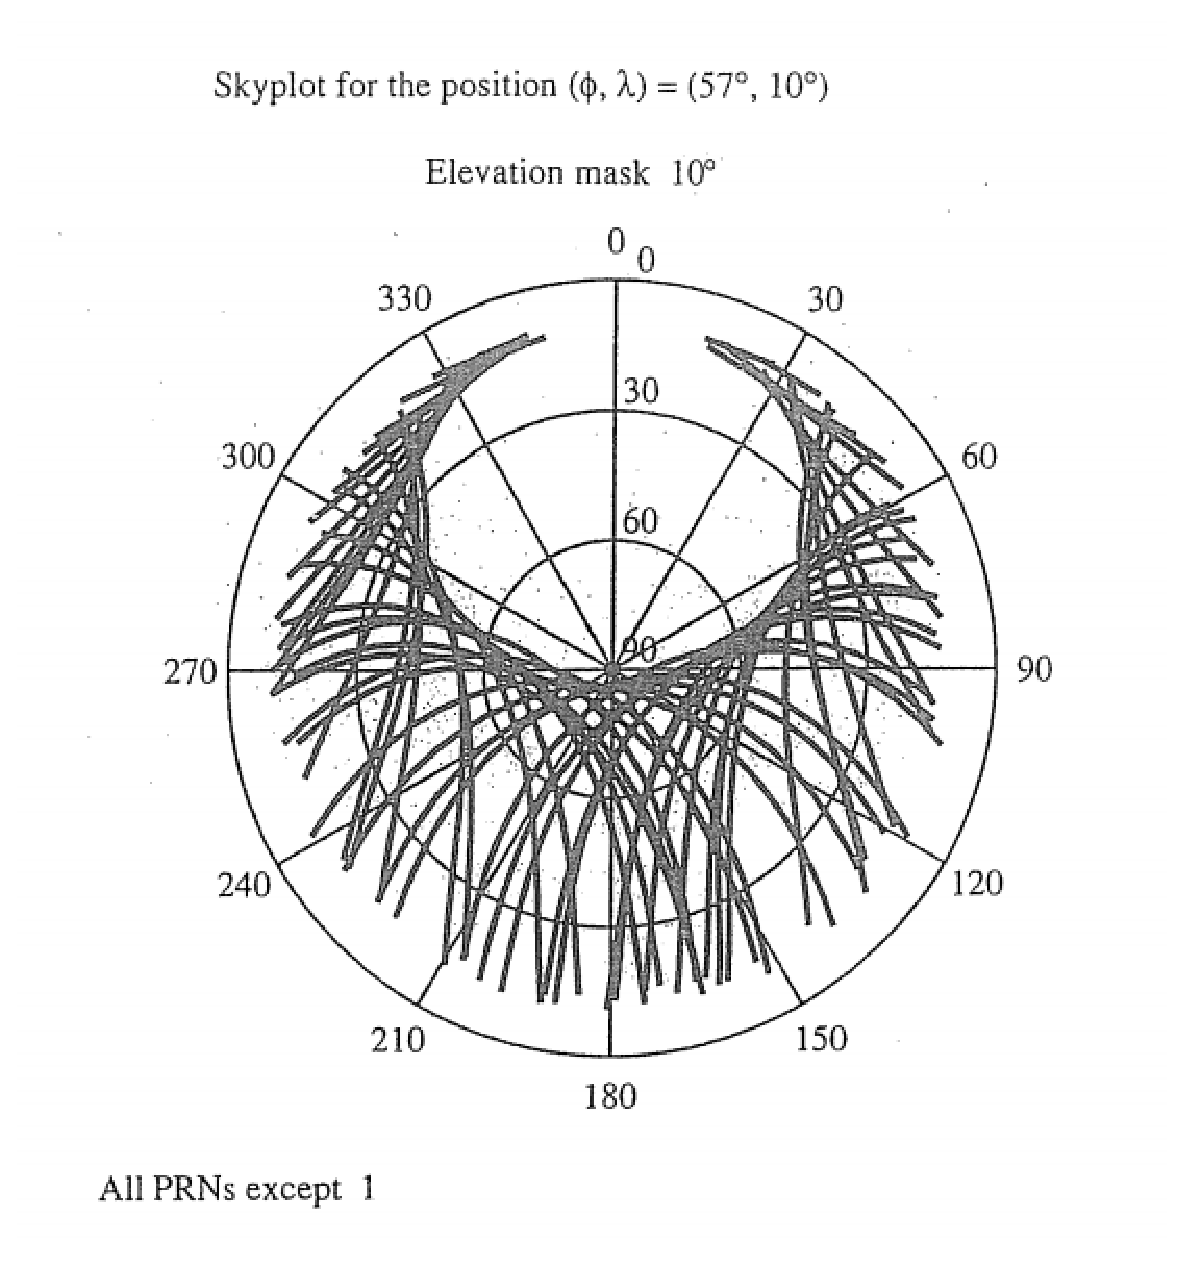
\includegraphics[width=0.7\linewidth]{TeX_files/Part03/chapter09/image/9-9}
		\caption{天空图包括所有GPS卫星在24小时内的给定位置。所有的高度角都为$10^\circ$。其中仅不包含1号卫星。}
		\label{fig:9-9}
	\end{figure}
	
	说一下卫星的星历表。这些参数值在一个特定的时间。每颗卫星传送其独特的星历数据。参数的描述实际的GPS卫星轨道及其开普勒轨道扰动参数。广播星历表使用之前直接计算轨道的一部分,和他们预测的下一个轨道的一部分。广播星历表是准确为1-2米。对于某些大地测量程序更好的精确性是必要的。一种可能性是获取精度在分米级的后处理精密星历表。
	
	星历表是用于从引用计数在GPS周秒时代t,它意味着间隔中心的星历是可用的。广播星历表的目的是在这段时间内使用。他们描述的是轨道2小时之后在指定位置的精度。他们预测4到6小时的曲线拟合数据。广播星历表包括
	
	$$\mu_0,\Delta n,e,\sqrt{a},\Omega_0,i_0,\omega,\dot{\Omega},\dot{i},C_{\omega c},C_{\omega s},C_{rs},C_{ic},C_{is},t_{oe}$$
	 
	在$\dot{\Omega}=\partial \Omega / \partial t$和$\dot{i}=\partial i / \partial t$。系数$C_\omega$,$C_r$,和$C_i$正确的近地点,轨道半径,由于不可避免的扰动理论和轨道倾角变化造成的轨道,地球的重力场,反射率和太阳的光压,太阳和月亮和潮汐力。星历表参数的参考时间是$t_{oe}$。
	
	考虑到传输时间t(在GPST时间)下面提供必要的变量供式\ref{eq:9.12}使用:
	\begin{table}
		\begin{tabularx}{\textwidth}{XX}
			\hline 过去的时间 $t_oe$  & $t_j=t-t_{oe}$ \\ 
			在$t_j$的平近点角 & $\mu_j = \mu_0 + (\sqrt{GM/a^3}+\Delta n)t_j$ \\ 
			地球的引力常数乘以质量 & $GM=3.986005\cdot 10^{14}M^3/S^2$ \\ 
			$E_j$的迭代解决方案  & $E_j=\mu_j+e\sin E_j$ \\ 
			真近点角  & $f_j=\arctan \dfrac{\sqrt{1-e^2}\sin E_j}{\cos E_j-e}$ \\ 
			升交点经度  & $\Omega_j=\Omega_0 + (\dot{\Omega_0}-\omega_e)t_j-\omega_et_{oe}$ \\ 
			地球平均自转   & $\omega_e=7.292115147\cdot10^{-5}rad/s$ \\ 
			近地点角距  & $\omega_j=\omega+f_j+C_{\omega c}\cos2(\omega+f_j)+C_{\omega s}\sin2(w+f_j)$ \\ 
			径向距离  & $r_j = a(1-e\cos E_j)+C_{rc}\cos 2(\omega+f_j)+C_{rs}\sin 2(\omega+f_j)$ \\ 
			轨道倾角  & $i_j = i_0+\dot{i}t_j+C_{ic}\cos 2(\omega+f_j)+C_{is}\sin 2(\omega+f_j)$ \\ 
			\hline 
		\end{tabularx} 
	\end{table}
	
	计算(9.12)的算法在M文件satpos中。函数计算GPS卫星的位置。它是每个位置计算的基础。为更多的细节在WGS84与GPS,见3.6节。
	
	这个m文件satposin计算卫星位置在一个惯性坐标系$\omega_e$ = 0中。
	
	关于开普勒元素的所有信息都包含在星历表。文件通过广播星历表时创建的GPS观测数据下载到一台笔记本电脑中。这些文件通常是特定的二进制格式。幸运的是可以转化为RINEX格式,这些格式见Gurtner(2000)。文件的后缀名第三个字符总是n(导航文件)。
	
	通常我们只需要导航信息中的一部分文件的星历文件。选择和重新格式化是通过以下命令:
	\begin{lstlisting}
	rinexe(ephemerisfile,outputfile);
	eph=get_eph(outputfile);
	satp=satpos(t,eph);
	\end{lstlisting}	
	\subsection[例子2]{例子2\\easy2}\label{subsec:easy2}
		第二个基本问题是计算以地球中心的惯性坐标系(ECI)中的给定位置的卫星伪距发出的时间。ECI GPS坐标系统使用地球赤道平面的方向是UTC时间2000年1月1日12时。x轴指向春分,z轴点北极的方向,y在是选为右手坐标系。
		\begin{figure}
			\centering
			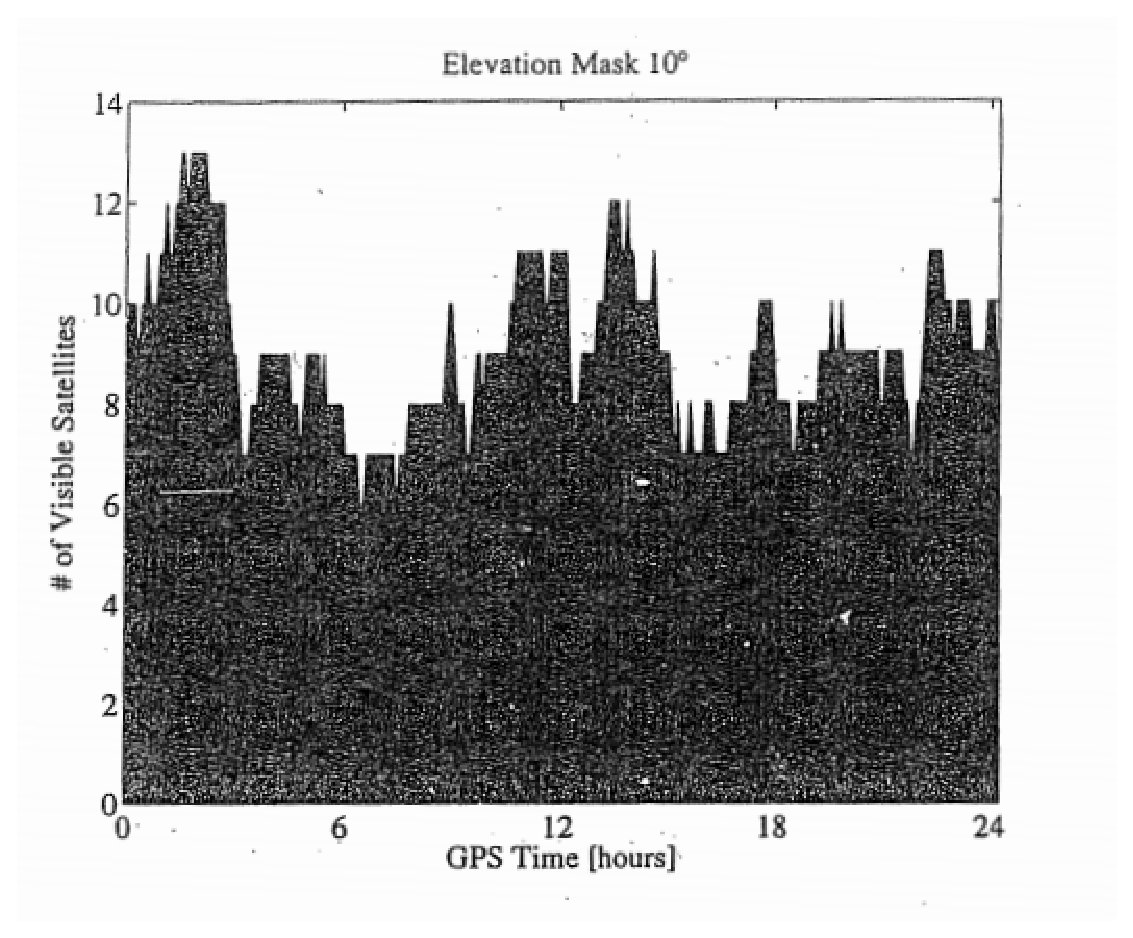
\includegraphics[width=0.7\linewidth]{TeX_files/Part03/chapter09/image/9-10}
			\caption{卫星高度角为$10^\circ$时}
			\label{fig:9-10}
		\end{figure}
		
		给定一个星历表从RINEX获得导航信息文件(n文件),easy2完成这个工作。主函数satpos实现GPS接口控制文档中描述的程序(IS-GPS-200 (2007)),表20-IV。
		
		我们读了RINEX格式的n文件,然后格式化成内部格式的MATLAB矩阵名叫Eph。此外,我们把Eph中的每一个卫星打印成一列。每一列包含21个变量;这些组成一个完整的卫星星历表一。
	
	\subsection[例子11]{例子11\\easy11}\label{subsec:easy11}
		图\ref{fig:9-9}展示了卫星轨道的极坐标图在一个地球上给定的位置。你可以看到的时间连续24小时期间每个卫星都是可见的。
		\begin{figure}
			\centering
			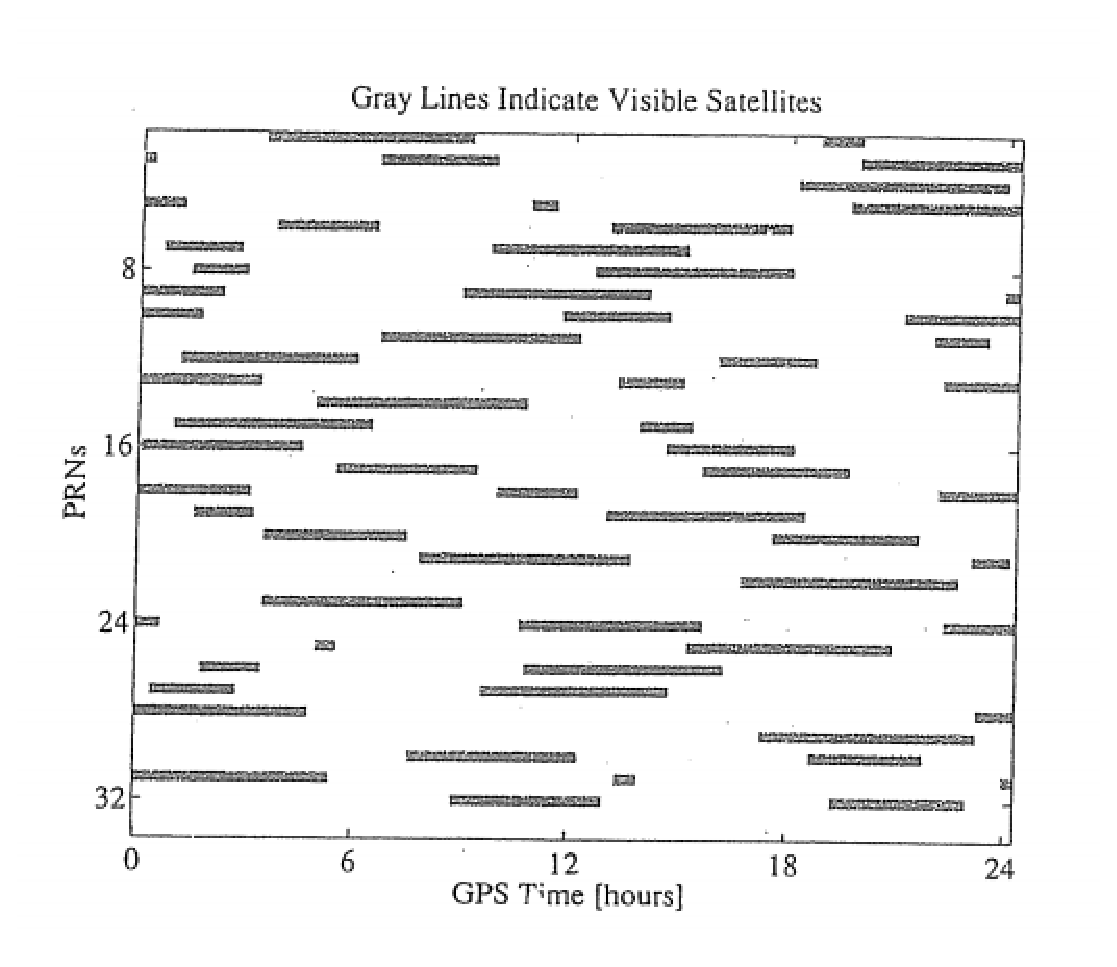
\includegraphics[width=0.7\linewidth]{TeX_files/Part03/chapter09/image/9-11}
			\caption{高度角大于等于$10^\circ$在 $\varphi = 57^\circ$和$\lambda = 10^\circ$位置的卫星}
			\label{fig:9-11}
		\end{figure}
		
		easy11是基于历书下载的最方便的国家大地测量服务ngs.noaa.gov/CORS/Data.html。实际的文件名是brdcl550.08n。
		
		MATLAB的RINEX文件已被重新格式化为二进制格式的卫星星历表,以提供给M文件rinexe使用。用户输入$(\varphi,\lambda)$的位置可以看到在这点的图像和一个需要设置的海拔值,然后将绘制所有可见的方位角和高度角的位置以及卫星计算和绘制极坐标。
		
		下一个遵循记录有多少,哪些卫星可见白天时间当他们可以看到。 图\ref{fig:9-10}和\ref{fig:9-11}将显示这些点。
		
		MATLAB代码很简单,结果令人印象深刻,它是有用的。在早期GPS星座是不完整的。这样的程序尤其有价值,为达成计划的目的是确保足够的卫星可以定位。除了最严重的地形和城市峡谷,接收器可以找到大量的GPS和GLONASS卫星,这种情况会在伽利略卫星发射后变得更加令人满意。
	

		\section[使用观测码定位接收机]{使用观测码定位接收机\\Receiver Position From Code Observations}
	在GPS接收机位置问题如下:卫星跟踪数$m\geq4$。我们假设在任何时间可以计算接收机的坐标。所有卫星和未知位置(X,Y,Z)接收机之间的距离。接收机的时钟是不精确的,所以我们也必须估算其和GPST相比的偏差$dt$。
	
	有四个未知数$X,Y,Z,dt$所以我们为了获得一个位置必须追踪至少四颗卫星。通常我们跟踪8到10颗卫星。
	
	GPS文献提到了几种方法来解决这个问题。普通最小二乘法是一种合理的选择。有的建议对观测到的接近天顶的卫星加权,例如Euler$\&$Goad (1991)。在1990年代Clyde Goad建议搜索在所有可能的位置找到平方和最小的误差。1985年Bancroft概述了基于内积方法,它假定m = 4。Kleusberg 在1994年描述了一个方法,消除了dt和观测方程的平方,再一次m = 4。这样的假设是没有预测到的今天有如此多的卫星。
		
	
	考虑一个GPS信号从卫星k到接收机$i = 1$ 通常$k = 1,……,m$。信号发出时间$t^k$由卫星时钟测定。到达时间$t^i$由接收机时钟测定。传播时间是$\tau^k_i$。如果c是光速,那么伪距$P^k_i$被定义为
	\begin{equation}\label{eq:9.13}
	t_i-t^k=\tau^k_i=P^k_i/c\quad or\quad t^k=t_i-P^k_i/c
	\end{equation}
	时钟并不准确,所以我们定义时钟偏移$dt$:
	接收机钟差
	\begin{equation}\label{9.14}
	t_i = t^{GPST}+dt_i
	\end{equation} 
	卫星钟差 $dt^k$:
	\begin{equation}\label{eq:9.15}
	t^k = (t-\tau ^k_i)^{GPST}+dt^k
	\end{equation}
	卫星时钟校正定义的参数在星历表上有 $a_0$,$a_1$,$a_2$ :
	\begin{equation}\label{eq:9.16}
	dt^k=a_0+a_1(t^k-t_{oe})+a_2(t^k-t_{oe})^2+\ldots
	\end{equation}
	使用$dt^k$后卫星钟的误差在$\pm 10$ns而且通常在$|dt_i|<1$ms.
	
	历元$t_i$定义为接收机的时刻。这个历元可见的所有的收到的信号来自跟踪的卫星。然而,信号的传输时间为$(t-\tau ^k_i)^{GPST}$,其中最重要的是$\mu ^k_i$换句话说就是从接收机i到卫星k的时间。因此首要任务是计算卫星k的传输时间$t^k$,这一步使用方程\ref{eq:9.15}和\ref{eq:9.16}。
	\begin{figure}
		\centering
		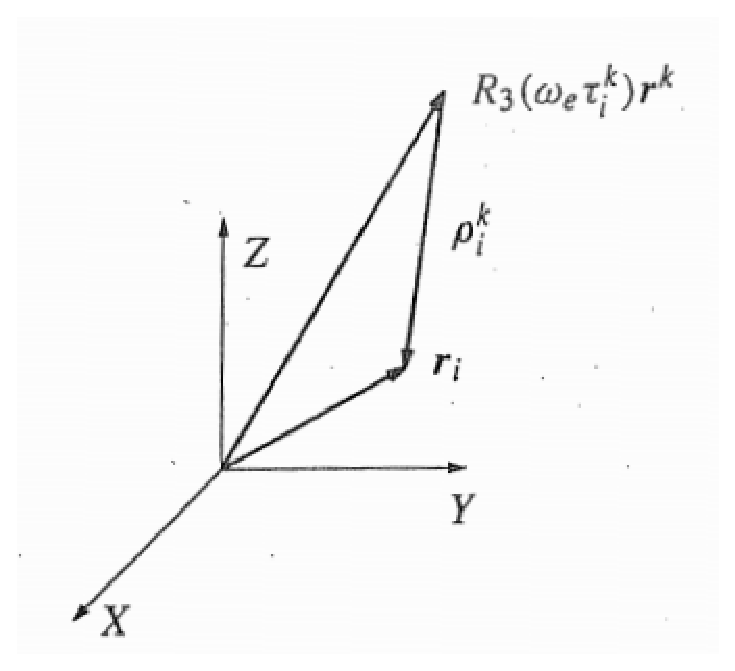
\includegraphics[width=0.7\linewidth]{TeX_files/Part03/chapter09/image/9-12}
		\caption{接收机坐标$r_i$在地心惯性坐标系和卫星坐标$R_3(\omega_e \tau ^k_i)r^k$在地心地固坐标系。 第一个位置是变成ECEF系统在z轴旋转的角度是$\omega_e \tau ^k_i$}
		\label{fig:9-12}
	\end{figure}
	
	根据星历表,所有卫星位置的计算在WGS-84坐标系钟,这是一个地心地固坐标系(ECEF)。这意味着我们必须旋转的卫星位置向量的三个轴向,相当于地球的角位移信号的传播从卫星到接收机。GPS卫星的高度约为20000公里。因此,信号传输时间是66ms。地球每自转$15arcsec$的角位移信号相当于地球的旋转轴的传播$1arcsec$。如果使用ECEF坐标并且没有调整,接收机坐标将偏向约相等于$1arcsec$的经度。
	
	依照图\ref{fig:9-12}卫星k和接收机i的距离对地球自转改正被定义为
	\begin{equation}\label{eq:9.17}
	\rho ^k_i = \Arrowvert R_3(\omega_e\tau^k_i)r^k(t-\tau^k_i)_{inert}-r_i(t)_{ECEF} \Arrowvert = 
	\Arrowvert \begin{bmatrix}
	X^k \\ Y^k \\ Z^k
	\end{bmatrix}-
	\begin{bmatrix}
	X_i \\ Y_i \\ Z_i
	\end{bmatrix} \Arrowvert
	\end{equation}
	
	矩阵$R_3$定义的旋转角度$\omega_e \tau^k_i$当信号传播时为:
	\begin{equation}\label{eq:9.18}
	R_3(\omega_e\tau^k_i) =
	\begin{bmatrix}
	\cos(\omega_e\tau^k_i) & \sin(\omega_e\tau^k_i) & 0 \\
	-\sin(\omega_e\tau^k_i) & \cos(\omega_e\tau^k_i) & 0 \\
	0 & 0 & 1
	\end{bmatrix}
	\end{equation}
	
	信号传播时间从(信号发出)卫星k到(信号接受)接收机i被表示为$\tau$。地球自转速率是$\omega_e$。ECEF系统中的位置向量表示为$r(t)_{ECEF}$。参数t强调对时间的依赖。
	
	伪距观测的基本方程的样子为:
	\begin{equation}\label{eq:9.19}
	P^k_i(t) = \rho^k_i+I^k_i+T^k_i-c(dt^k(t-\tau^k_i)-dt_i(t))-e^k_i
	\end{equation}
	
	电离层延迟为$I^k_i$,对流层延迟为$T^k_i$,c表示真空中的光速$e^k_i$表示一个错误。
	\begin{figure}
		\centering
		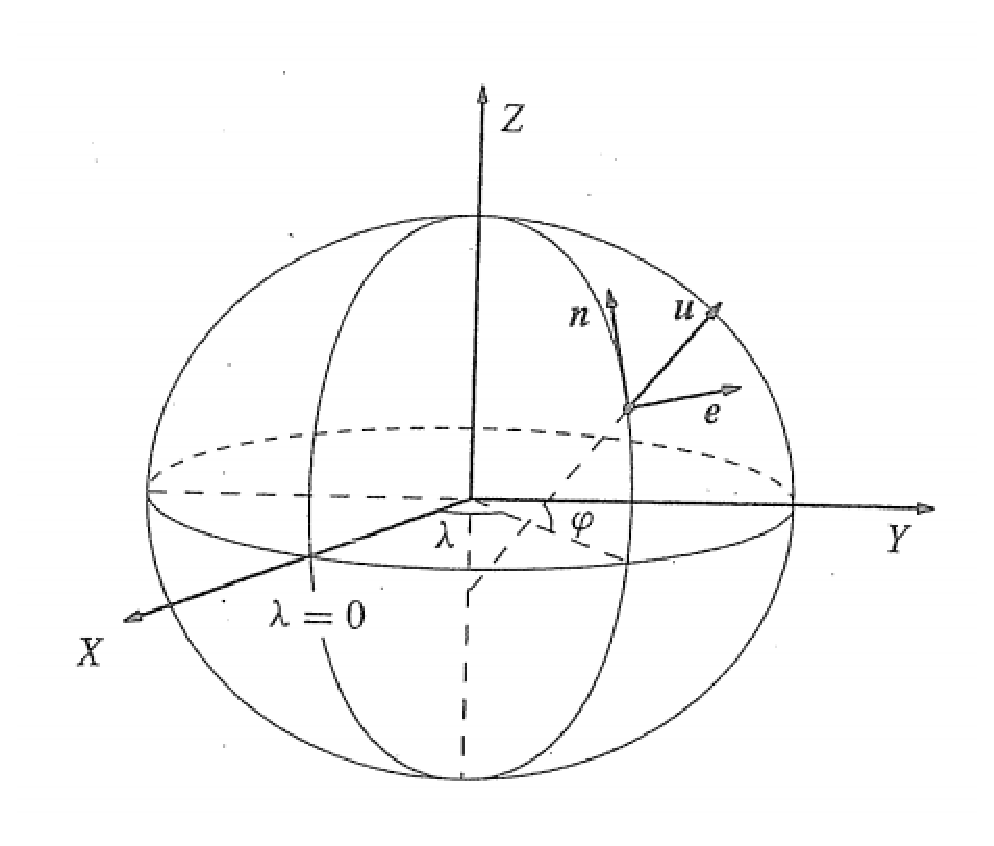
\includegraphics[width=0.7\linewidth]{TeX_files/Part03/chapter09/image/9-13}
		\caption{站心坐标系(e,n,u)}
		\label{fig:9-13}
	\end{figure}
	
	所以我们需要改变一个站心坐标系的向量x到当地的e,n坐标系,u为铅锤线方向,n指向北,e指向西,在图\ref{fig:9-13}中显示。 站心坐标系由地心矢量给出X,和三个单位向量的正交矩阵F已经介绍在(3.31)中介绍。
	\begin{equation}\label{eq:9.20}
	F = \begin{bmatrix}
	e & n & u
	\end{bmatrix}=
	\begin{bmatrix}
	-\sin \lambda & -\sin\varphi\cos\lambda & \cos\varphi\cos\lambda \\
	\cos \lambda & -\sin\varphi\sin\lambda & \cos\varphi\sin\lambda \\
	0 & \cos\varphi & \sin\varphi
	\end{bmatrix}
	\end{equation}
	
	知道笛卡尔坐标的初值$(X^0_i,Y^0_i,Z^0_i)$我们就可以计算接收机的地理坐标$(\varphi,\lambda)$,因此获得矩阵F。现在让$(E,N,U)=F^Tx$。我们立即获得方位角、高度角和距离:
	\begin{table}
		\begin{tabular}{ll}
			 方位角: 		 & $Az = \arctan(E/N)$ \\ 
			 高度角:		 & $El=\arctan(U/\sqrt{N^2+E^2})$ \\ 
			 距离: 		  & $s=\Arrowvert x \Arrowvert$ \\ 
		\end{tabular} 
	\end{table}
	
	知道高度角我们可以计算$T^k_i$。电离层延迟$I^k_i$设置为0,因为我们不知道更好的值,$dt^k$的值由式\ref{eq:9.16}计算得出。未知数$dt_i$和三维坐标$(X_i,Y_i,Z_i)$是隐藏在$\rho^k_i$。所以我们先线性化式\ref{eq:9.19}:
	\begin{equation}\label{eq:9.21}
	-\dfrac{X^k-X^0_i}{(\rho^k_i)^0}x_i-\dfrac{Y^k-Y^0_i}{(\rho^k_i)^0}y_i-\dfrac{Z^k-Z^0_i}{(\rho^k_i)^0}z_i+1(c\,dt_i)=(P^k_i)_{obs}-(P^k_i)^0-e^k_i=b_i-e^k_i
	\end{equation}
	
	第一个近似值我们设为 $\rho^k_i\approx(\rho^k_i)^0=(P^k_i)^0$,通过几何距离的近似值计算卫星和接收机的坐标。$b_i$表示观测值减去计算值。
	
	$(P^k_i)^0$的初值可能是源自或从可能的接收机的初步计算坐标$(X^0_i,Y^0_i,Z^0_i)$获得。这是修正接收机时钟偏移 $dt_i$,与第一个估计值$dt_i=0$。如果初值好则右侧$b_i$很小。注意方向余弦描述的参数使用式\ref{eq:9.17}。
	
	描述线性化观测方程的式子是\ref{eq:9.21}我们设置的未知数是$x=(x_i,y_i,z_i,c\,dt_i)$:
	\begin{equation}\label{eq:9.22}
	Ax=\begin{bmatrix}
	-\dfrac{X^1-X_i}{\rho^1_i} & -\dfrac{Y^1-Y_i}{\rho^1_i} & -\dfrac{Z^1-Z_i}{\rho^1_i} & 1 \\
	-\dfrac{X^2-X_i}{\rho^2_i} & -\dfrac{Y^2-Y_i}{\rho^2_i} & -\dfrac{Z^2-Z_i}{\rho^2_i} & 1 \\
	\vdots & & & \\
	-\dfrac{X^3-X_i}{\rho^3_i} & -\dfrac{Y^3-Y_i}{\rho^3_i} & -\dfrac{Z^3-Z_i}{\rho^3_i} & 1 \\
	\end{bmatrix}
	\begin{bmatrix}
	x_i \\ y_i \\ z_i \\ c\,dt_i
	\end{bmatrix}
	= b-e
	\end{equation}
	
	注意参数c和$dt_i$一起呆在在一个产品中。这样做是为了数值的原因。未知的$c\,dt_i$和另一未知数有着一样的维度,即长度。然而有些人喜欢随着时间估计。这可以通过使用未知的$dt_i$一起相当小系数$c x 10^9$收益率$dt_i$ns。???
	
	Row-wise包含前三列向量的方向余弦在卫星和接收机之间。最小二乘的解决方案是
	\begin{equation}\label{eq:9.23}
	\begin{bmatrix}
	\hat{x}_i \\ \hat{y}_i \\ \hat{z}_i \\ \widehat{c\,dt_i}
	\end{bmatrix}
	=(A^T\Sigma^{-1}A)^{-1}A^T\Sigma^{-1}b
	\end{equation}
	
	伪距观测值被认为是独立等效的方差$e\sim N(0,\sigma^2I)$。换句话说矢量e零均值和协方差矩阵$\Sigma=\sigma^2I$。如果这个假设是正确的,式\ref{eq:9.23}可以化简为
	\begin{equation}\label{eq:9.24}
	\begin{bmatrix}
	\hat{x}_i \\ \hat{y}_i \\ \hat{z}_i \\ \widehat{c\,dt_i}
	\end{bmatrix}
	=(A^TA)^{-1}A^Tb
	\end{equation}
	迭代接收机坐标
	\begin{equation}\label{eq:9.25}
	\hat{X}_i=X^0_i+\hat{x}_i,\quad \hat{Y}_i=Y^0_i+\hat{y}_i,\quad and \quad \hat{Z}_i=Z^0_i+\hat{z}_i,
	\end{equation}
	迭代涉及式\ref{eq:9.22},\ref{eq:9.24} 和 \ref{eq:9.25} 重复直到稳定 $\Arrowvert x\Arrowvert=\sqrt{x^Tx}$ 小于 $10^2$,可以说
	
	最后我们建立一个数据集组成的一个历元。它包含$PRN`s k = 1,4,7,13,20,24,25$在表\ref{tab:9.4}。伪距改正是根据以下方程:
	\begin{equation}\label{eq:9.26}
	P = observed\,pseudorange + c\,dt^k-T.
	\end{equation}
	
	M-文件easy3是调用satpos在传输时间的计算。
	\begin{table}
		\caption{坐标$(X^k,Y^k,Z^k)$ 卫星出现在一个特定的历元。观测到的伪距用$P^k$表示}
		\label{tab:9.4}
		\begin{tabular}{crrrr}
			\hline
			PRN & 1 & 4 & 7 & 13 \\ 
			\hline
			$X^k[m]$ & 14789533.14 &  11784778.93 &  20131229.62 & 22053478.89  \\ 
			$Y^k[m]$ &  7334543.20 & -10589833.27 & -17092167.32 & -4245955.78  \\ 
			$Z^k[m]$ & 20976503.11 &  21427005.76 &   1367264.01 & 14103264.45  \\ 
			$P^k[m]$ & 20589966.21 &  21428477.36 &  24767161.79 & 21266276.50  \\ 
			\hline
		\end{tabular} 
		\begin{tabular}{crrr}
			\hline
			PRN & 20 & 24 & 25 \\
			\hline
			$X^k[m]$ & 12654506.52 &  -1514708.63 & -9091147.00 \\
			$Y^k[m]$ & 17685295.10 & -16394944.97 & 13349830.35 \\ 
			$Z^k[m]$ & 15150460.02 &  21142855.83 & 21347346.61 \\ 
			$P^k[m]$ & 21871195.29 &  23851770.76 & 24109819.35 \\ 
			\hline
		\end{tabular}
	\end{table}	
	
	\begin{figure}
		\centering
		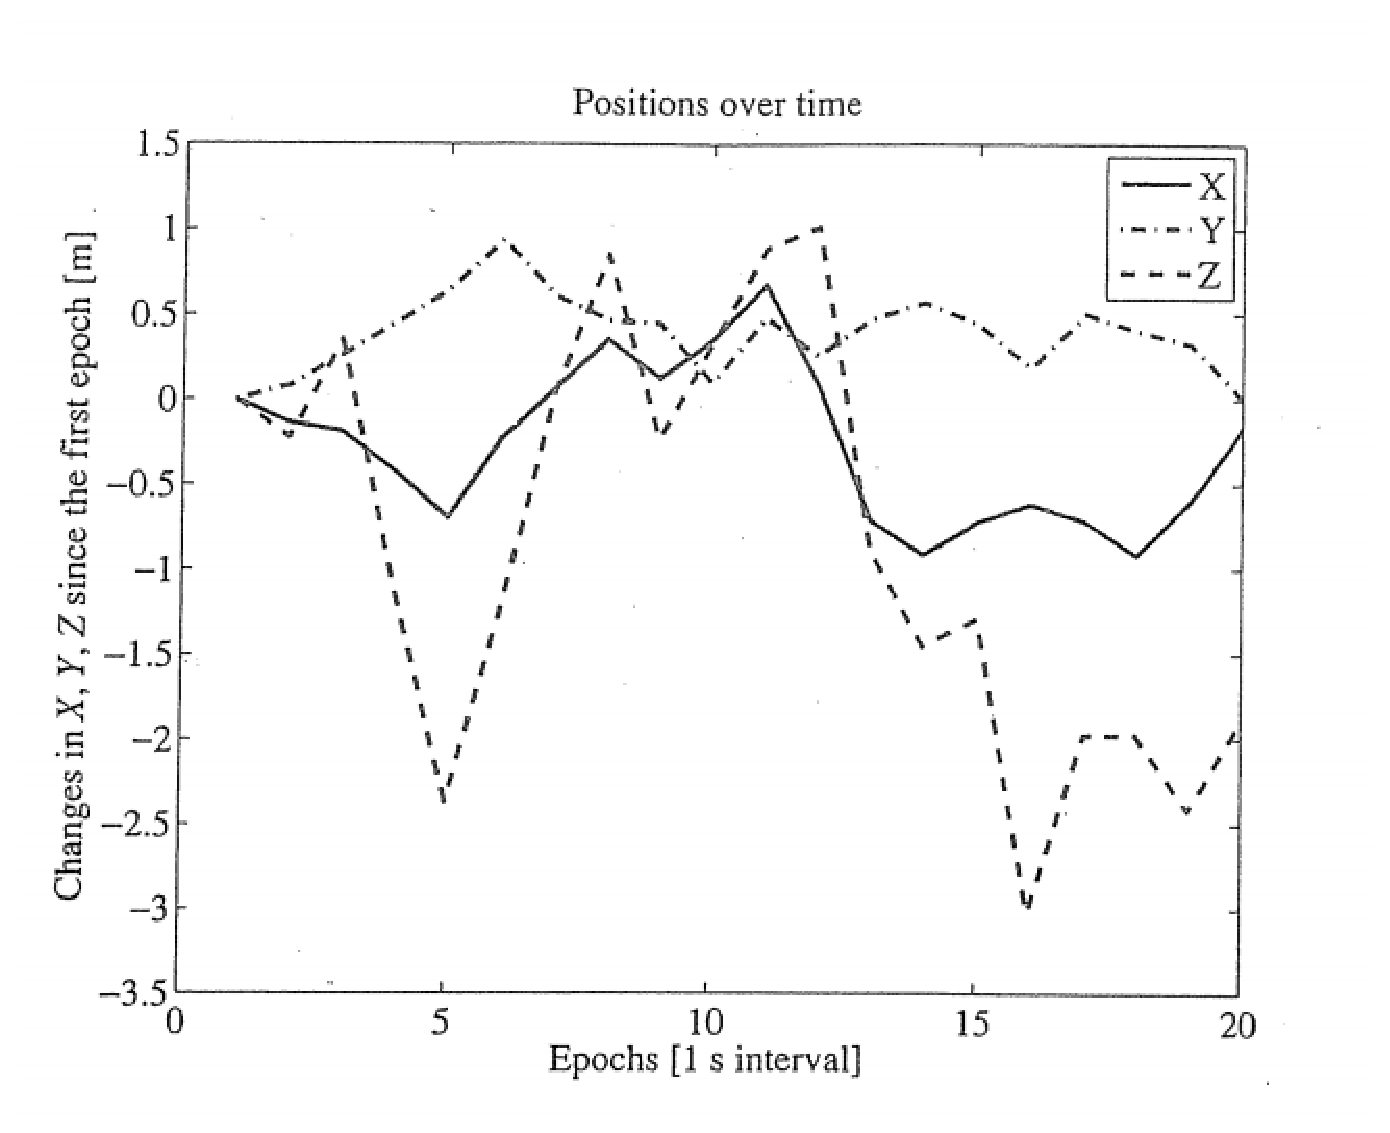
\includegraphics[width=0.7\linewidth]{TeX_files/Part03/chapter09/image/9-14}
		\caption{随时间变化由伪距得出的接收机坐标:X,Y,Z}
		\label{fig:9-14}
	\end{figure}
	
	知道卫星位置和测量的伪距我们可以估计接收机坐标和接收机时钟偏移量$\widehat{c\,dt}$通过最小二乘法:
	
	接收机的时钟偏移量和GPS时间相比为$\widehat{dt} = 0.377 ms$。6次迭代后得到的结果。接收机位置的标准差是2.3米,详见第四章。

	\subsection[例子3]{例子3\\easy3}\label{subsec:easy3}
		在easy3中我们通过O文件和N文件计算了接收机的ECEF坐标,仅仅使用了伪距值。GPST的传播时间是$(t_i-\tau^k_i)^{GPST}$ 用于计算卫星位置。
		
		接下来我们引用一个中心块的代码应用于任何位置计算。第一次可能很难阅读,但是我们试着把单词:目标是找到一个特定的历元在GPST从给定的卫星信号传播。我们知道历元 $t_i$、计算的接收机时钟,当观察值被确定。有信号传播$P/c$秒之前的卫星。我们知道了伪距P和光速c。接下来,我们计算的卫星时钟偏移tcorr参数$a_0$和$a_1$的星历表。然而,这个量取决于星历的时间发布在tOc。所以tcorr的值只能通过迭代,所以你看tcorr出现在左边的两倍。我们终于可以知道tcorr在那一刻计算的真实GPST信号传播时最后卫星的位置。代码如下:
		\begin{lstlisting}
		k = col_Eph(i);
		tx_RAW = time - obs(i)/v_light;
		tOc = Eph(21,k);
		dt = check_t(tx_RAW-tOc);
		tcorr = (Eph(2,k) * dt + Eph(20,k)) * dt + Eph(19,k);
		tx_GPS = tx_RAW- tcorr;
		dt - check_t(tx_GPS-tOc);
		tcorr = (Eph(2,k) * dt -f Eph(20,k)) * dt + Eph(19,k);
		tx_GPS = tx_RAW-tcorr;
		X = satpos(tx_GPS, Eph(:,k));			
		\end{lstlisting}
		下面的代码纠正地球自转导致的信号传播从卫星到接收机的误差。式\ref{eq:9.18}中描述卫星的位置必须在z轴旋转角$\omega_e\tau^k_i$。在第一个迭代中我们不知道确切的传播时间并将其设置为0.072秒。对流层延迟设置为0s。我们在下一次迭代估计卫星的仰角,作为这个角el计算对流层延迟是很重要的。它是实现对流层的代码。
		\begin{lstlisting}
		if iter == 1
			traveltime = 0.072;
			Rot_X = X;
			trop = 0;
		else
			rho2=(X(1)-pos(1))~2+(X(2)-pos(2))~2+(X(3)-pos(3))~2;
			traveltime = sqrt(rho2)/v_light;
			Rot_X = e_i'_corr(traveltime,X);
			rho2 = (Rot_X(l)-pos(1))^2 + (Rot_X(2)-pos(2))"2-r (Rot_X(3)-pos(3))^2;
			[az,el,dist] = topocent(pos(1:3 /:),Rot_X-pos(1:3,:));
			if iter == nojterations, El(i) = el; end
			trop=tropo(sin(el*dtr),0.0,1013.0,293.0,50.0,0.0,0.0,0.0);
		end
		\end{lstlisting}
		接收机的位置计算的关键代码是一个单独的m文件$recpo_ls$.
		
		我们打开一个RINEX格式的O文件读取所有的伪距。从easy2与给定的卫星位置,我们计算出接收机的位置。
		
		重复计算了20个历元。每个位置是迭代最小二乘的结果的过程。位置相对于第一个历元的变化如图\ref{fig:9-14}。坐标的变化值一般小于5米。
		
		
	


		\section[可选择的算法]{可选择的算法\\Alternative Algorithms}
	我们考虑各种最小二乘的模型:为了估计接收机j的坐标,通过给出的卫星位置坐标和伪距我们认为普通最小二乘法和加权最小二乘法模型最适合。下面是基于数值的例子显示在表中\ref{tab:9.4}。这个计算在rp.m文件中被实现。
	\subsection[普通最小二乘]{普通最小二乘\\Ordinary Least Squares}
	这个模型描述了$Ax=b+e$。A中每一行的内容为:
	\begin{equation*}
		\begin{bmatrix}
		
		-\dfrac{X^k-X_i}{\rho^k_1} & -\dfrac{Y^k-Y_i}{\rho^k_1} & -\dfrac{Z^k-Z_i}{\rho^k_1} & 1
		
		\end{bmatrix}
	\end{equation*}
	对应 $b_k$ 的 b 是:
	\begin{equation*}
		P^k - \Arrowvert 
		\begin{bmatrix}
			X^k & Y^k & Z^k
		\end{bmatrix}-
		\begin{bmatrix}
		
		X & Y & Z
		
		\end{bmatrix}
		\Arrowvert_2
		-c\,dt
	\end{equation*}
	经过6次迭代后结果如下:

	\begin{align*}
		\hat{X} = 3427824.23 \\
		\hat{Y} =  603665.35 \\
		\hat{Z} = 5326882.42 \\
		\hat{c\,dt} =  113058.30
	\end{align*}
		与标准偏差为 2.3 m.
	\subsection[加权最小二乘]{加权最小二乘\\Weighted Least Squares}
	可以说,高度角较大的卫星的伪距观测较高度角较小的卫星更精确。让$a_0$和$a_1$作为常数,追踪高度角为h的卫星,高度角的截止角度为$h_0$。然后一个标准模型差为$\sigma_b = a_0 + a_1e^{-h/h_0}$。但是我们使用一个更简单的表达式$\sigma_b=1/\sin h$。权$c_i$通过$c_i=1/\sigma^2_b$计算得出。加权调整的结果为:
		\begin{align*}
			\hat{X} = 3427826.07 m \\
			\hat{Y} =  603664.47 m \\
			\hat{Z} = 5326883.17 m \\
			\hat{c\,dt} = 113059.57 m.
		\end{align*}

	偏离不超过1-2米的每个卫星未加权的结果是。单位权的标准差下降至0.7米。
	\subsection[结论]{结论\\Conclusions}

	一组的高斯方法设置了m个方程和n个未知数,m>n,两个历元后仍保持不变。如下

		\begin{itemize}

			\item 一个独特的(加权)与最小方差最小二乘解

			\item 测量的准确性(协方差)的解决方案。

		\end{itemize}

	在早期的GPS,m和n往往是一个比较小的整数。计算设备的能力是有限的,所以它自然成为寻找最优的解决方案。最常见的选项是放弃一部分。现在我们做得更好。

	示例9.1(精度因子)协方差$matrix_{ECEF}$ for $(x_i,y_i,z_i,c\,dt)$包含的信息决定几何定位的质量。$\Sigma$是更小的($\hat{x}$更精确的)卫星间隔。追踪$\Sigma_{ECEF}$压缩这个信息到一个数字,我们不能恢复置信椭球。坐标追踪系统和四个差异$\sigma^2_X+\sigma^2_Y+\sigma^2_Z+\sigma^2_{c\,dt}$,是独立的坐标系统。除了几何信息这些差异包括观测的准确性。
这可以由$\sigma^2_0$消除。
	
	我们从协方差矩阵的最小二乘问题开始\ref{eq:9.22}:

		\begin{equation}\label{eq:9.27}
			\Sigma_{ECEF} = 
			\begin{bmatrix}

				\sigma^2_X & \sigma_{XY} & \sigma_{XZ} & \sigma_{X,c\,dt} \\

				\sigma_{YX}& \sigma^2_Y  & \sigma_{YZ} & \sigma_{Y,c\,dt} \\

				\sigma_{ZX}& \sigma_{ZY} & \sigma^2_Z & \sigma_{Z,c\,dt} \\

				\sigma_{c\,dt,X} & \sigma_{c\,dt,Y} & \sigma_{c\,dt,Z} & \sigma^2_{c\,dt} 

			\end{bmatrix}
		\end{equation}

	传播规则将$\Sigma_{ECEF}$转换为本地系统中表达的协方差矩阵坐标(E,N,U)。有趣的是3×3子矩阵S$\Sigma_{ECEF}$在\ref{eq:9.27}所示。转换矩阵是$F^T$,这个子矩阵S是:

		\begin{equation}\label{eq:9.28}
			\Sigma_{ENU} = 
			\begin{bmatrix}

				\sigma^2_E & \sigma_{EN} & \sigma_{EU} \\

				\sigma_{NE}& \sigma^2_N  & \sigma_{NU} \\

				\sigma_{UE}& \sigma_{UN} & \sigma^2_U \\
			\end{bmatrix}
			=F^TSF
		\end{equation} 

	F连接笛卡尔坐标和本地坐标系统的差异(纬度$\varphi$和经度$\lambda$)和ECEF坐标系,参考(3.28)这是衍生出的另一种方式。序列(E,N,U)确保当地和ECEF系统应当是右手坐标系:

		\begin{equation}\label{eq:9.29}
		\begin{array}{rcl}

			F^T &=& R_3(\pi)R_2(\varphi-\frac{\pi}{2})R_3(\lambda-\pi) \\

				&=&\begin{bmatrix}

						0 & -1 & 0 \\

						1 &  0 & 0 \\

						0 &  0 & 1

					\end{bmatrix}

					\begin{bmatrix}

					\sin \varphi & 0 & \cos \varphi \\

					0 & 1 & 0 \\

					-\cos \varphi& 0 & \sin \varphi

					\end{bmatrix}

					\begin{bmatrix}

					-\cos \lambda & -\sin \lambda & 0 \\

					\sin \lambda & -\cos \lambda & 0 \\

					0 & 			0 & 1 

					\end{bmatrix} \\

				 &=&\begin{bmatrix}

					-\sin \lambda & \cos \lambda & 0 \\

					-\sin \varphi \cos \lambda & -\sin \varphi \sin \lambda & \cos \varphi \\

					\cos \varphi \cos \lambda & \cos \varphi \sin \lambda & \sin \varphi 

					\end{bmatrix}
		\end{array}	
		\end{equation}
	在实践中我们遇到一些形式的精度因子(缩写为DOP):

		\begin{table}

			\begin{tabularx}{\textwidth}{lX}

				几何精度因子: & $GDOP=\sqrt{\sigma^2_E+\sigma^2_N+\sigma^2_U+\sigma^2_{c\,dt}}/\sigma_0=\sqrt{trace(\Sigma_{ECEF})}/\sigma_0$ \\

				水平精度因子:&$HDOP=\sqrt{\sigma^2_E+\sigma^2_N}/\sigma_0$ \\

				位置精度因子:  & $PDOP=\sqrt{\sigma^2_E+\sigma^2_N+\sigma^2_U}/\sigma_0=\sqrt{\sigma^2_X+\sigma^2_Y+\sigma^2_Z}/\sigma_0=\sqrt{trace(\Sigma_{ENU})}/\sigma_0 $ \\

				时间精度因子:	   &$TDOP=\sigma_{c\,dt}/\sigma_0$ \\

				垂直精度因子:  &$VDOP=\sigma_U/\sigma_0$ 

			\end{tabularx}

		\end{table}

	注意,所有DOF值是无量纲的。他们用错误的范围表示位置的错误(大约)。而且我们有

		\begin{equation*}
			GDOP^2=PDOP^2+TDOP^2=HDOP^2+VDOP^2+TDOP^2
		\end{equation*}

	DOP值在规划观测时间是特别有用的。为此目的的历书没有比广播星历表更高的精度。历书数据允许预先计算卫星位置在几周和有足够的准确性(轨道的星历表表示是在很短的时间内有效)。任何人使用全球定位系统(GPS)时DOP是一个有用的工具,在一些卫星星座比其他的已知最好的卫星覆盖的时候。???

	经验表明,良好的观测是位置误差$PDOP<5$,测量来自至少五个卫星。

	备注9.1伪距观测b是未知的接收机坐标的非线性函数。我们主要线性化观测值和使用泰勒级数展开。
		\begin{equation*}
			b=b_0+(X-X_0)^Tgrab\,b|_{X=X_0}+\frac{1}{2}(X-X_0)^TH|_{X=X_0}(X-X_0)+\ldots
		\end{equation*}

	$X_0$和$X$的是在展开点计算的,和Hessian H是二阶导数。我们的目标是估计二阶项的大小。这一项告诉我们关于截断一阶项后的系数的误差。对一组伪距这导致使用张量,所以我们开发一个简单的例子中,使用一个伪距为b。
			
	我们已经知道的梯度中给定的伪距\ref{eq:9.22}我们省略和时钟偏移相关的最后一列:

		\begin{equation}\label{eq:9.30}
			A=\begin{bmatrix}
			-\dfrac{X^1-X_i}{\rho^1_i} & -\dfrac{Y^1-Y_i}{\rho^1_i} & -\dfrac{Z^1-Z_i}{\rho^1_i}
			\end{bmatrix}
		\end{equation}

	二阶导数在Hessian收集:

		\begin{equation}\label{eq:9.31}
			H=
			\begin{bmatrix}

				\dfrac{(Y^1-Y_i)^2+(Z^1-Z_i)^2}{(\rho^1_i)^3} & \dfrac{(X^1-X_i)(Y^1-Y_i)}{(\rho^1_i)^3} 		& \dfrac{(X^1-X_i)(Z^1-Z_i)}{(\rho^1_i)^3} \\

				\dfrac{(X^1-X_i)(Y^1-Y_i)}{(\rho^1_i)^3}       & \dfrac{(X^1-X_i)^2+(Z^1-Z_i)^2}{(\rho^1_i)^3}   & \dfrac{(Y^1-Y_i)(Z^1-Z_i)}{(\rho^1_i)^3} \\

				\dfrac{(X^1-X_i)(Z^1-Z_i)}{(\rho^1_i)^3} 	  & \dfrac{(Y^1-Y_i)(Z^1-Z_i)}{(\rho^1_i)^3} 		& \dfrac{(X^1-X_i)^2+(Y^1-Y_i)^2}{(\rho^1_i)^3}		
			\end{bmatrix}
		\end{equation}

	和

		\begin{align*}
			X^1=(-9138250.97,13331687.71,21338151.79)^T \\
			X_0=(3427823.97,603665.739,5326881.602)^T
		\end{align*}

	和$\alpha=\frac{1}{2}(X-X_0)^TH(X-X_0)$我们从下表中获得数据:
		\begin{table}

			\begin{tabular}{cccc}

				\hline

				$X-X_0[m]$ & (1,1,1) & (100,100,100) & (10000,10000,10000) \\ 

				$\alpha [m]$ & $3\times10^{-8}$ & $3\times10^{-4}$ & 3.02 \\ 

				\hline

			\end{tabular} 

		\end{table}

	任何模棱两可的成功解决方案取决于伪距观测值;我们目睹,忽略二阶项在正常情况下是无风险的!

			


		\section[搜索定位接收机]{搜索定位接收机\\Receiver Position by Search}
	我们描述一个搜索过程,解决了最小二乘问题没有形成正常的方程。假设四个或更多伪距美元$P_1,P_2,\vdots,P_m$在同一历元。我们要确定我们的接收机的位置,没有先验知识,它的位置。
		
	首先我们计算ECEF坐标的m卫星星历文件。然后wc的笛卡尔坐标变换每个卫星传输时间(可以从伪距获得)到 $(\varphi_i,\lambda_i)$ = (纬度,经度)。平均坐标是我们第一次猜的接收机的位置。
		
	以这个点为中心,我们引入一个网格覆盖一个半球。可能将$\pi/2$十等分,可能16等分$2\pi$的角度。在每个网格点,我们计算剩余 $R_i=P_i-P_1,i=2,\vdots,m $,观察到的伪距之间的差异和第一个值来消除接收机时钟偏移量。接下来我们区分这些差异:
	\begin{align*}
		r_1& = R_2-R^0_2 = (P_2-P_1) - (P^0_2-P^0_1) \\
		r_2& = R_3-R^0_3 = (P_3-P_1) - (P^0_3-P^0_1) \\
		\vdots& \\
		r_{m-1}& = R_m-R^0_m = (P_m-P_1) - (P^0_m-P^0_1) 
	\end{align*}
	\begin{figure}
			\centering
			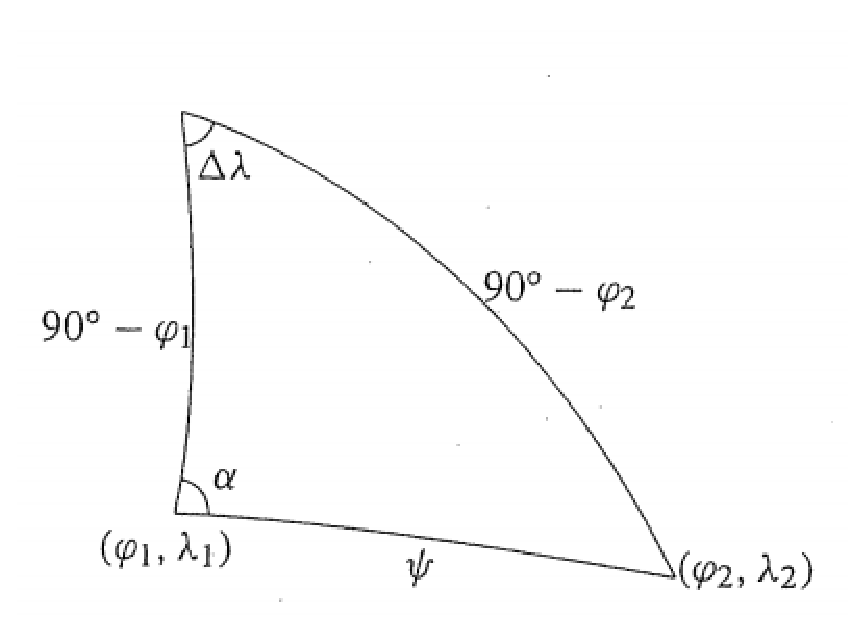
\includegraphics[width=0.7\linewidth]{TeX_files/Part03/chapter09/image/9-15}
			\caption{球面三角形计算接收机的纬度和经度 $(\varphi,\lambda)$}
			\label{fig:9-15}
	\end{figure}

	这给第一个近似和$S=\Sigma r^2_i$之间的所有S的可能值,现我们寻求最小的一个,现与该值是新的接收机的位置的估计值。网格是为更精细的下一次迭代。现一个新的决定和选择如下,细化网格的中心和一个后续的搜索。重复这个过程,直到没有进一步改善位置。

	最后,我们展示如何计算球面三角学的新位置,如图\ref{fig:9-15}。最初点的坐标 $(\varphi_1,\lambda_1)$。我们想要移动$\psi$度沿方位角$(\varphi_2,\lambda_2)$的方向。计算$\varphi_2$和$\lambda_2$是一个经典大地测量问题,以下基本方程产生解决方案在球面上:
	\begin{equation}\label{eq:9.32}
		\sin\varphi_2 = \sin\varphi_1\cos\psi+\cos\varphi_1\sin\psi\cos\alpha\quad and \quad \sin\Delta\lambda=\dfrac{\sin\aleph\sin\psi}{\cos\varphi_2}
	\end{equation}

	这些方程给出新的点的纬度 $\varphi_2$和增量$\Delta\lambda$的经度。的m文件recpos显示了快速的实现代码。最终找到一个接收器位置与轨道的精度一致,折射模型和伪距。
		
	这是另一个最小二乘的一个例子。这里,由于$P_1$减去其他伪距,这显然是相关的差异。任何错误在$P_1$出现在每一个差异中。在搜索中我们忽略这些相关性,因为这个过程只是为了给第一次估计的接收机的位置。
		
	使用适当的协方差矩阵最小二乘过程应该遵循我们的搜索技术。由此产生的猜测是几乎总是(线性)收敛区域内。获得的导航数据rinexe $('ohiostat.96n','rinex_n.dat')$。你可以放大图片按下鼠标按钮。许多你可以读出缩放后的x和y标签的位置。

	将$get_eph$m文件打开,读取和构造一个星历表文件。这样的文件通常包含几个特定卫星数据集。常见的做法是选择立即时代之前的星历表使用。文件$find_eph$便是这个用途。然而保持这种做法,最终导致星历数据的变化。这很可能会引入跳轨道计算。更先进的程序平滑轨道,如果他们需要更长时间的使用。一个更好的解决方案是改用精密星历表。

		\section[GPS观测值的误差项]{GPS观测值的误差项\\Errors in the GPS Observables}

	\subsection[信号的延迟]{信号的延迟\\Delay of the Signal}
	
	\subsection[GPS误差预算]{GPS误差预算\\Error Budget for GPS}
	
	\subsection[例子16]{例子16\\easy16}\label{subsec:easy16}
	
	\subsection[例子10]{例子10\\easy10}\label{subsec:easy10}
	
	\subsection[误差预算的汇总]{误差预算的汇总\\Summary of the Error Budget}
	

		\section[星基增强系统]{星基增强系统\\Satellite Based Augmentation Systems}
	
	\subsection[测距修正和检测站]{测距修正和监测站\\Ranging and Integrity Monitoring Station}
	
	\subsection[SBAS消息和产生]{SBAS消息和产生\\SBAS Messages and Their Generation}
	
	\subsection[总结SBAS修正]{总结SBAS修正\\Summary of the SBAS Corrections}
	
	\subsection[例子13]{例子13\\easy13}\label{subsec:easy13}
	
	\subsection[例子14]{例子14\\easy14}\label{subsec:easy14}
	
	\subsection[伽利略完整性的概念]{伽利略完整性的概念\\The Galileo Integrity Concept}
	

		\section{Quality Control}
Data processing can be performed as non-recursive (batch least-squares) or as recursive
least-squares estimation. This section contains a brief description of the models involved
and the related procedures for testing and reliability. A typical example is the situation
of possible cycle slips in the carrier phase observation. The alternative hypotheses may
consist of cycle slips in GPS carrier observations.
	\subsection{The Non-Recursive Case}
	In hypothesis testing, one usually calls the case without any model errors the null hypoth-esis $H_0$. An alternative hypothesis $H_a$ assumes there is a bias in one or several of the
	observations. Let c be a known m-vector specifying the model error, x be the n-vector of
	unknowns and s its unknown size. Then two hypotheses are defined as
	\begin{equation}
	H_0: b=Ax+e  \qquad weight\,C=\Sigma^{-1}_b
	\end{equation}
	\begin{equation}
	H_a:b=Ax+sc+e  \qquad weight\,C=\Sigma^{-1}_b.
	\end{equation}
	We assume that $m > n$.
	
	Assuming each alternative hypothesis describes the case of a single bias in an observation, the c-vectors consist of canonical unit vectors. The solution to (4.101) under the null hypothesis is given by
	\begin{equation*}
	\begin{split}
	\hat{x}&=(A^TCA)^{-1}A^TCb\\
	\Sigma_{\hat{x}}&=(A^TCA)^{-1}
	\end{split}.
	\end{equation*}
	Testing $H_0$ against $H_a$ consists of three steps:
	
	Detection\; An overall model test determines if unspecified model errors have occurred.
	
	Identification\; If a model error is detected, its potential source is identified by testing the
	original or nominal observation model (4.101) against models extended with bias	parameters, such as (4.102). 
	
	Adaptation \; After the identification of the most likely source for the model error, the observation model is adapted to eliminate the biases in the parameter vector.
	
	The projector $P=I-(A^TCA)^{-1}A^TC$ projects vectors onto the column space of
	A as demonstrated in Section 6.6. The vector of residuals is $\hat{e}=b-A\hat{x}$.
	
	In the detection step the uniformly most powerful test statistic for testing $H_0$ against
	$H_a$ is given as 
	\begin{equation}
	T=\frac{(Pb)^TCb}{m-n}=\frac{\hat{e}^TC\hat{e}{m-n}}.
	\end{equation}
	T is the overall model test statistic. Under $H_0$ and $H_a$, T is F distributed:
	\begin{equation*}
	H_0:T~F(m-n,\infty ,0) \qquad H_a:T~F(m-n,\infty ,\lambda)
	\end{equation*}	 
	The non-centrality parameter $\delta$ is defined as
	\begin{equation}
	\delta=s^2c^TCPc.
	\end{equation}
	Once reference values are chosen for the level of confidence $\alpha_0$ (the probability of rejecting $H_0$ falsely), the detection power $\gamma_0$(the probability of rejecting $H_0$  when $H_a$ is true) and the number of degrees of freedom m — n, the non-centrality parameter $\delta$ can be computed. This is the B-method of testing which was described by Willem Baarda in 1968.
	
	The B-method assumes that an error related to the non-centrality parameter $\delta_0=\delta(\alpha_0,\gamma_0,1)$ is detected with equal probability $\alpha$ by all tests. In other words from $\delta_0=\delta(\alpha_0,\gamma_0,1)=\lambda(\alpha,\gamma_0,m=n)$, with $m-n>1$, the level of confidences $\alpha$ can be computed.
	Once $\delta_0$ is known, the size of the bias that can just be detected follows from (4.104) as
	\begin{equation}
	|s|=\sqrt{\frac{\delta_0}{c^TCPc}}.
	\end{equation}
	This is the Minimal Detectable Bias (MDB). As can be seen from (4.105), the MDB depends on $\alpha_0,\gamma_0$, and the functional and stochastic model, through the design matrix A and
	the covariance matrix $\Sigma_b$ and the alternative hypothesis captured in the vector c.
	
	Remark 4.4\; We bring a detailed description of a procedure for computation of the non-centrality parameter $\delta$.
	
	First the central case (null hypothesis $H_0$): select a value for a which is the probability of an error of the first kind, that is rejecting $H_0$ falsely.
	
	MATLAB uses left tail and we need right tail, so we define $p=1-\alpha$. The number
	of degrees of freedom is f = m - n. The critical value is computed as x = chi2inv(p,f).
	This is the value where the critical region starts (rejection of $H_0$) and extends to $+\infty$.
	
	Next the non-central case (alternative hypothesis $H_a$): We know the critical value x
	and the number of degrees of freedom f, and must solve p = ncx2cdf (x,f,delta ) iteratively
	such that $\delta$ yields the known value for p.
	
	The solution from this iteration yields $\beta=p$(left tail probability of accepting $H_0$,
	while $H_0$ is true). The probability of correct decision is the “power” $\gamma=1-\beta$.
	
	For most GPS applications we set $\alpha_0=0.001,\gamma_0=0.80$ (or even higher) resulting
	in a non-centrality parameter of $\delta_0\approx 17$, see Figure 4.13. The computation is done by the M-file cct.
	
	\begin{figure}[h]
		\centering
		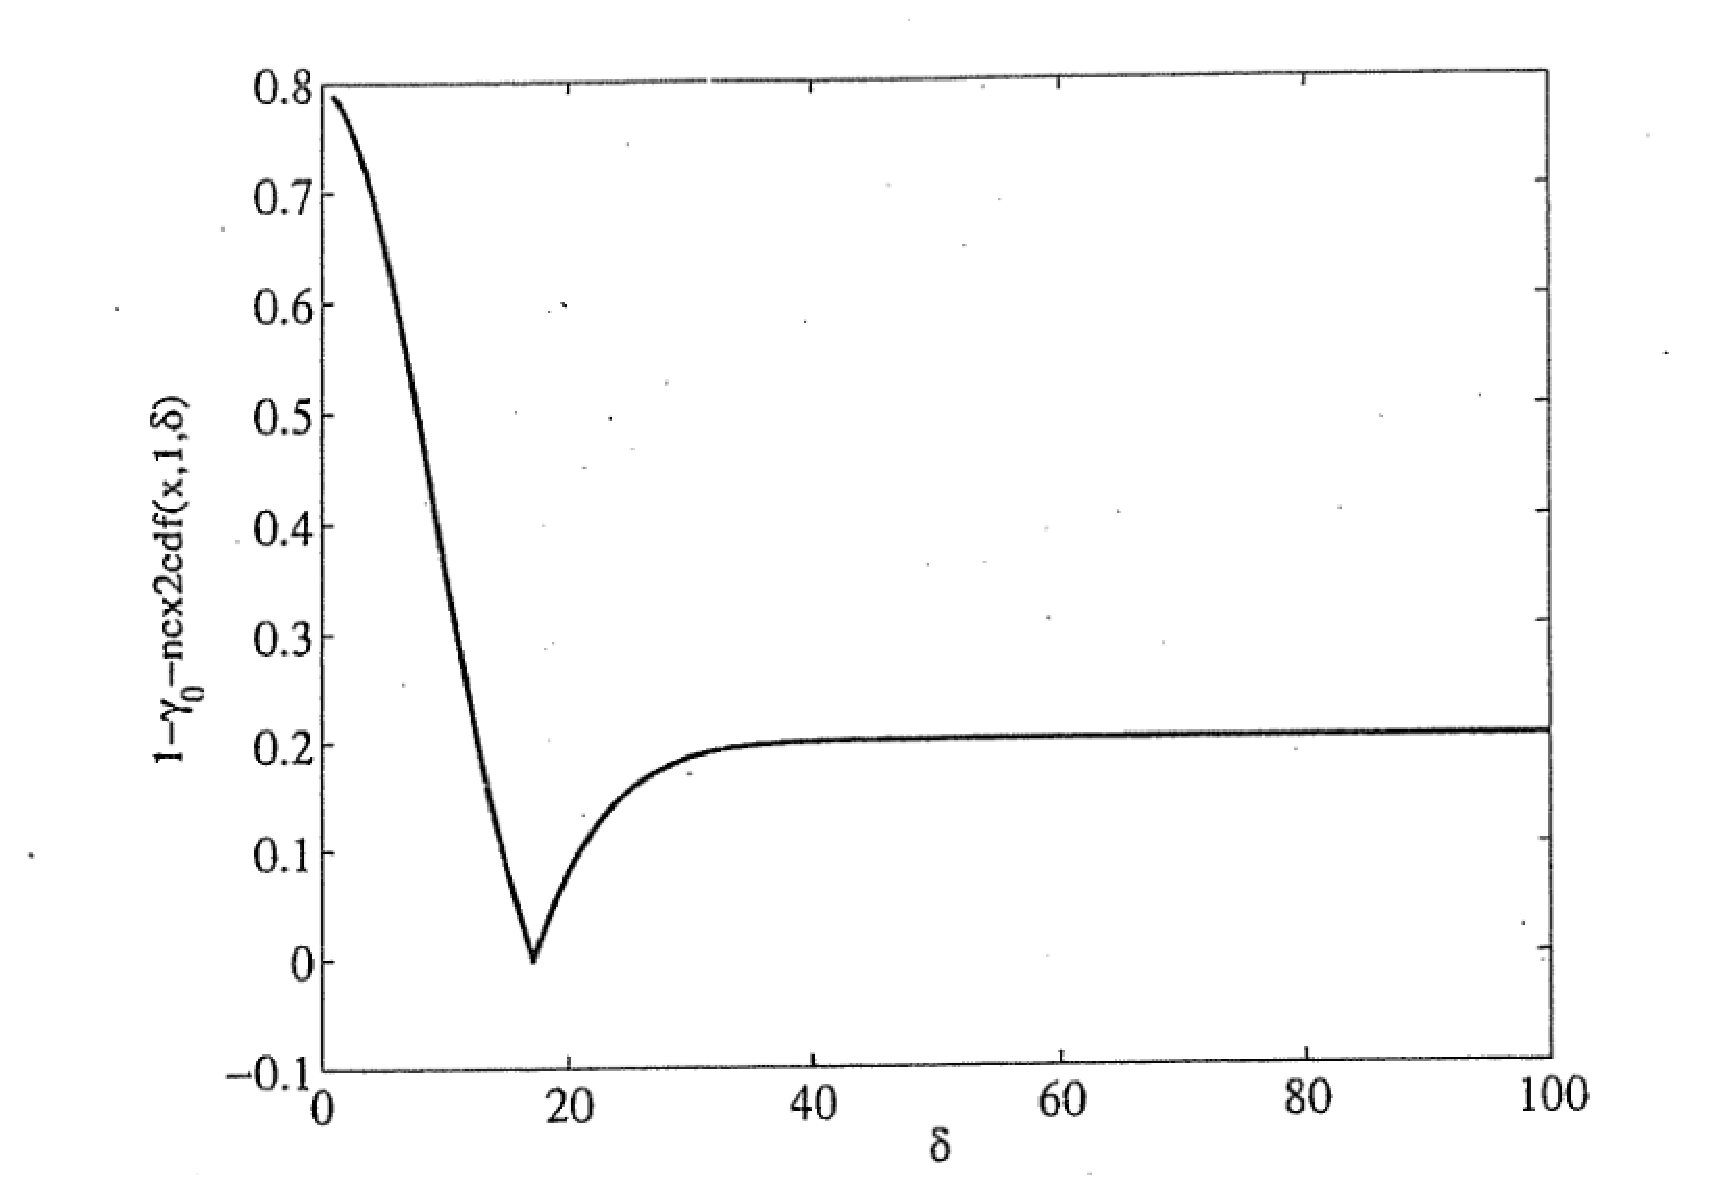
\includegraphics[width=0.7\linewidth]{TeX_files/Part02/chapter04/image/4-13}
		\caption{Figure 4.13\; The function $1-\gamma_0-ncx2cdf(x,1,\delta)$ as function of $\delta$}
		\label{fig:4-13}
	\end{figure}
	
	If the test statistic T exceeds a threshold, we say we have detected a bias s and
	the sources of the possible errors have to be found in the identification step. In practice
	this is accomplished by testing a number of alternative hypotheses, each describing one
	model error at a time, see (4.102). The uniformly most powerful test statistic for testing
	$H_0$ against $H_a$ is given as
	\begin{equation}
	t=\frac{(Pc)^TCPb}{\sqrt{(Pc)^TCPc}}=\frac{c^TCPb}{\sqrt{c^TCPc}}.
	\end{equation}
	This expression is known as a slippage test statistic. Under $H_0$ and $H_a$ the slippage test
	statistic is normally distributed
	\begin{equation*}
	\begin{split}
	 &H_0:t~N(0,1)   \\
	 &H_a:t~N(\sqrt{(Pc)^TCPc}s,1).
	\end{split}
	\end{equation*}
	The practical procedure for identifying model errors is to determine the largest slippage test statistic (in absolute value) and perform another least-squares adjustment until the
	test statistic T is accepted, or until there is no redundancy left, i.e., until m - n = 0 . Once the largest slippage test statistic t has been found, its likelihood needs to be tested. The	likelihood of the identified model error can be tested by comparing the test statistic with the critical value $N_{\alpha_0/2}(0,1)$ where $\alpha_0$ is the level of confidence. If the largest slippage test statistic t in each cycle exceeds the critical value, i.e, if
	\begin{equation*}
	|t|>N_{\alpha_0/2}(0,1)
	\end{equation*}
	then it is likely that a model error has been identified. If not, one should extend the set of alternative hypotheses to consider.
	
	For the adaptation step, several alternatives exist. One way to adapt would be to
	simply discard the bad observations (as already done, actually, in the iterated identification
	step), another to extend the vector of unknowns by one or more additional parameters.
	
	The alternative hypotheses may consist of outliers and cycle slips in GPS code and
	carrier observations, respectively. The MDB is said to describe the internal reliability of
	a system. External reliability is defined as the influence of a bias s with size equal to the
	MDB on the estimated parameters sx:
	\begin{equation*}
	sx=(A^TCA)^{-1}A^TCcs=\Sigma_{\hat{x}}A^TCcs.
	\end{equation*} 
	It should be noted that to compute internal and external reliability parameters, no actual
	data is required. They can already be computed in the design or planning phase of a survey.
	
	\subsection{The Recursive Case}
	The main difference with non-recursive or batch least squares is that for recursive least
	squares the unknown parameters are updated whenever new observations become available. Assuming the unknown parameters remain the same for an entire observation period,
	the null and alternative hypothesis for an epoch k are defined as 
	\begin{equation*}
	\begin{split}
	&H_0:b_k=A_kx   \\
	&H_a:b_k=A_kx +s_kc.
	\end{split}
	\end{equation*}
	Here we assume that a bias $s_k$ is detected and identified at the same epoch it occurred.
	in other words, we consider only local alternative hypotheses as opposed to global ones,
	which consider a number of (or even all) epochs before detecting and identifying the bias.
	Assuming a solution $\hat{x}_{k|k-1}$ with covariance matrix $P_{k|k-1}$ is available (where the subscript (k - 1) means that all epochs up to and including k - 1 were used to compute
	this solution), the recursive solution for k epochs of data under the null hypothesis is given
	as
	\begin{equation*}
	\hat{x}_{k|k}=\hat{x}_{k|k-1}+K_k(b_k-A_k\hat{x}_{k|k-1}) 
	\quad and \quad
	P_{k|k}=(I-K_kA_k)P_{k|k-1}
	\end{equation*}
	with
	\begin{equation*}
	K_k=P_{k|k-1}A^T_k(A_kP_{k|k-1}A^T_k+\Sigma_{e,k})^{-1}.
	\end{equation*}
	The vector
	\begin{equation}
	i-k=b_k-A_k\hat{x}_{k|k-1}
	\end{equation}
	is known as the innovation. Its covariance matrix is
	\begin{equation}
	\Sigma_i=A_kP_{k|k-1}A^T_k+\Sigma_{e,k}.
	\end{equation}
	Alternatively, the matrices $K_k$ and $P_{k|k}$ may be written as
	\begin{equation*}
	\begin{split}
	K_k &= P_{k|k}A^T_k\Sigma^{-1}_{e,k}\\
	P_{k|k} &=(P^{-1}_{k|k-1}+A^T_k\Sigma^{-1}_{e,k}A_k)^{-1}.
	\end{split}
	\end{equation*}
	Let $m_k$ be the number of observations at epoch k. For the detection and identification step,
	the local overall model test statistics T and local slippage test statistics t are given by
	\begin{equation*}
	\begin{split}
	&T=\frac{i^T_k\Sigma^{-1}_ii_k}{m_k}\\
	&t=\frac{c^T\Sigma^{-1}_ii_k}{\sqrt{c^T\Sigma^{-1}_ic}}
	\end{split}
	\end{equation*}
	which under $H_0$ and $H_a$ are distributed as
	\begin{equation*}
	H_0:T~F(m_k,\infty ,0) \qquad H_a:T~F(m_k,\infty ,\delta)
	\end{equation*}	
	and
	\begin{equation*}
	H_0:t~N(0,1) \qquad H_a:t~N(\sqrt{c^T\Sigma^{-1}_ic}s,1).
	\end{equation*}
	The expression for the MDB reads
	\begin{equation*}
	|s|=\sqrt{\frac{\delta_0}{c^T\Sigma^{-1}_ic}}.
	\end{equation*}
	The influence of a bias with size equal to the MDB on the estimated parameters is given as
	\begin{equation*}
	sx=sK_kc.
	\end{equation*}
	For further reading, see Teunissen \& Kleusberg (1998), Chapter 7 on “Quality Control and GPS .”
	

1\; For two independent measurements $x= b_1$ and $x= b_2$, the best $\hat{x}$ should be some
weighted average $\hat{x}=ab_1+(1-a)b_2$. When $b_1$ and $b_2$ have mean zero and
variances $\sigma^2_1$ and $\sigma^2_2$, the variance of $\hat{x}$ will be $P=a^2\sigma^2_1+(1-a)^2\sigma^2_2$. Choose the number a that minimizes P: dP/da = 0.

Show that this a gives the weighting which we have claimed to be best, using weights
$w_1=1/\sigma_1$ and $w_2=1/\sigma_2$.

2\; After N = 4 coin flips (binomial distribution) what are the five probabilities $p_0,p_1,...,p_4$ of M = 0,1,..., 4 heads? Find the mean $\bar{M}=\Sigma Mp_M$.
Show that the variance $\sigma^2=\Sigma(M-\bar{M})^2 p_M$ agrees with N/4 = 1.

3\; (a) At the center of Figure 4.3 with N = 4 and $\sigma^2=N/4 = 1$, check that the actual
height $p_2=\frac{6}{16}$ is a little below the Gaussian $p(x)=1/\sqrt{2\pi}\sigma$.

(b) The center of the Gaussian with $\sigma=\sqrt{N}/2$ has height $\sqrt{2\pi N}$. Using Stirling's approximation to N! and (N/2)!, show that the middle binomial coefficient $p_{N/2}$
approaches that height: 	
\begin{equation*}
(M=\frac{N}{2})   \quad p_{N/2}=\frac{N!}{((N/2)!)^2}\approx \frac{(N/e)^N\sqrt{2\pi N}}{((n/2e)^{N/2}\sqrt{\pi N})^2}=?
\end{equation*}	

4\; The variance $\sigma^2=\Sigma(n-\bar{n})^2p_n$  is computed around the mean $\bar{n}=\Sigma np_n$. Expand $(n-\bar{n})^2=n^2-2n\bar{n}+\bar{n}^2$ to show that this $\sigma^2$ equals $(\Sigma n^2p_n)-\bar{n}^2$.

5\; Imagine a line of masses $p_0,...,p_n$ at the points x = 0,...,n. Explain how the
mean $E\{x\}$ with probabilities $p_j$ corresponds to the center of mass. The variance $\sigma^2$
is the moment of inertia around what point?

6\; Start with r independent random variables $X_1,...,X_r$ with variances $\sigma^2_1,...,\sigma^2_r$. Show that the sum $X=X_1+...+X_r$ has variance $\sigma^2_1+...+\sigma^2_r$.

7\; One flip of a weighted coin has M = 1 (heads) with probability p and M = 0 (tails)
with probability q = 1 - p. What are the mean $\bar{M}$ and the variance $\sigma$? What are
the mean and variance for the number M of heads after N coin flips?

8\; Suppose every number is rounded down to the nearest integer. The distribution of
rounding errors e is still uniform, but on what interval of e's? What is the mean m?
What is the variance around the mean $\int(e-m)^2$ de?

9\; Suppose the random variable X has mean $\mu$ and variance $\sigma^2$.

(a) \; Show that the new variable Y = aX + b has mean $a\mu+b$.

(b) \; Show that the variance of Y is $a^2\mu^2$.

10\; Suppose X is a vector of random variables, each with mean zero, and Y = LX is
related to X by a fixed matrix L(m by n). Derive from (4.16) the “Law of Covariance
Propagation” which brings L and $L^T$ outside:
\begin{equation*}
\Sigma_Y=L\Sigma_XL^T \quad or \quad E\{YY^T\}=LE\{XX^T\}L^T.
\end{equation*}
Problems 11-14 give experience with a small-size Kalman filter

11\; In Example 4.6, extend the matrix A to 5 by 3 with $x_3-x_2=c_2$ and a new measurement
$x_3=b_3$. With unit variances in C = I, solve $A^TA\hat{x}=A^Tb$ for the best estimates $\hat{x_1},\hat{x_2},\hat{x_3}$.

Solution: With $c_1=c_2=0,\hat{x}_{3|3}=\frac{1}{8}(b_1+2b_2+5b_3)$ and $P_{3|3}=\frac{5}{8}$.

12\; In Problem 11, continue the Kalman recursion from $\hat{x_{2|2}}$ in the text to predict 
$\hat{x_{3|2}}$ and correct to $\hat{x_{3|3}}$. As in Example 4.7, find their variances $P_{3|2}$ and $P_{3|3}$ from the last entries in $(A^TA)^{-1}_{3|2}$ and $(A^TA)^{-1}$.

13\; In this Kalman example, the determinants of $A^TA$ come from the Fibonacci numbers
1,1,2,3,5,8,... as new rows are added to A. Find the three pivots of $(A^TA)_{3|3}$ as
ratios of Fibonacci numbers:
\begin{equation*}
A^TA=
\begin{bmatrix}
2&-1&0\\
-1&3&-1\\
0&-1&2
\end{bmatrix}
LDL^T  \quad with\,pivots\,in\,D.
\end{equation*} 	
14\; For $\sigma^2_1=\sigma^2_2=1$ and any $v^2_1$ in (4.31), the covariance matrix is $\Sigma=diag(1,v^2_1,1)$. Solve $A^T\Sigma^{-1}A\hat{x}=A^T\Sigma^{-1}b$. What are the limiting values of $\hat{x}_i$,as $v_1\rightarrow 0$?	
	%%----------------------------第九章结束-------------------------%%
	
	%%----------------------------第十章开始-------------------------%%
	\chapter[差分观测的一种方法]{差分观测的一种方法\\Differences of One-Way Observations}
	\minitoc %小标题
	\newpage%新页
		\section[联合观测的方法]{联合观测的方法\\Combining One-Way Observations}
单向码观测值是指一颗卫星和一台接收机间的观测值。计算一台独立接收机的位置需要4个或者更多的观测值。根据经验可知,相邻位置的误差源(比如大气延迟)是相同的。这就促使我们使用相邻两个接收机观测相同卫星的模型。此模型计算了两个接收机间的不同矢量。但是比起两个接收机位置相减的解法,这种方法并不会得到更好地结果。有时这种差分模型实际上会产生更差的结果。下面看easy4文件。

\subsection[例子4]{例子4\\easy4}
	easy4文件处理了两个接收机C/A伪距码的同步观测值。我们对两个天线的基线进行估计并在图\ref{fig:10-1}中画出了它的$(X,Y,Z)$分量。坐标变化量达到10m。因此,利用单伪距估计得到的天线位置和基线解有相同的噪声水平。这个结论仅对2000年3月2号之后的观测值有效。
	
	因此,如果对来自两个测站的同步观测数据进行处理,我们得到的基线精度是单点定位误差精度的$\sqrt{2}$倍,除非接收机观测到的伪距是负相关的。那么这种差分方法是不能改善这种情况的。
	
	只有通过使用最小二乘法程序对独立观测值(单向的)进行改正,才能提高差分向量的精度。这正是第九章提出的使用卫星地基增强系统(SBSA)的思想。当码观测值和调制在载波L1、L2上的相位观测值进行组合时,图像变化剧烈。这将在327???页做出总结。
	\begin{figure}
		\center{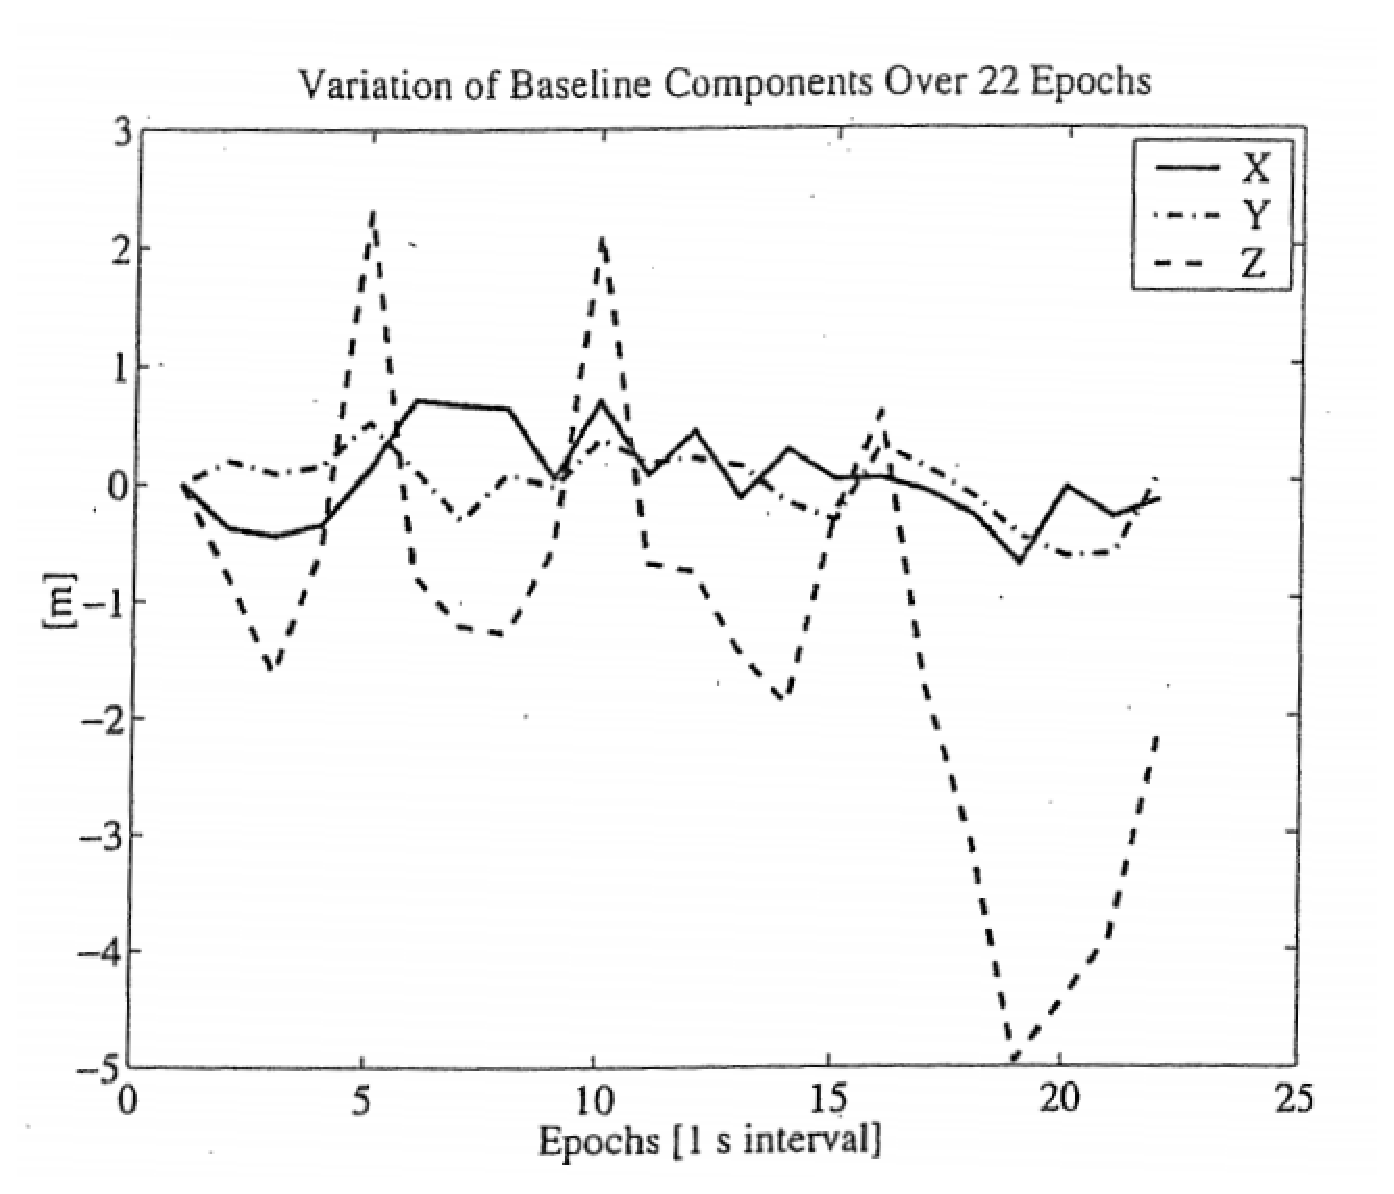
\includegraphics[width=10cm]  {TeX_files/Part03/chapter10/image/10-1.eps}}        
		\caption{ 利用两台接收机的伪距观测值估计得到的基线$(X,Y,Z)$随时间的变化}   \label{fig:10-1} 
	\end{figure}
	%CMD命令:bmeps -c inputFile.PNG outputFile.esp
	
	正如在 公式(10.2)???定义的,相位噪声$\epsilon$的标准差有几毫米,而伪距误差$\varrho$取决于接收机的质量。由于凿速率(频率的另一术语)变慢,C/A 码伪距的噪声值可以达到2$\sim$3m。P码的速率可以达到每秒1023万二进制数字或者每秒1023万位。凿速率是C/A码速率的10倍,这也暗示着P码的噪声水平在10$\sim$30cm。一个小的伪距标准差对快速固定L1,L2载波上的整周模糊度是至关重要的。P码通常是加密的,被称之为Y码。
	
	下面说明了双频接收机是如何工作的:C/A码仅调制在L1载波上,而P码既调制在L1载波上也调制在L2载波上。P码很长并且不是哥德尔序列(Gold码)。接收机利用C/A码实现与P码的同步,数据存储在导航信息中。因此,接收机只需要实现与C/A码的同步,同时解调导航信息,这与单频率接收机非常相似。在导航信息中可以找到记录一个移位寄存器当前内容的数据,这个移位寄存器用来生成P码。用这种方法就能实现P码的同步。现今的新科技允许获取P码或者是加密的Y码。更多细节详见Misra\&Enge(2006)。
	
	这章由以下组成:	
	\begin{itemize}
		\item 相位观测值;载波N的数量是未知的(模糊度)
		\item 周跳的检查;整周数N的变化
		\item 差分GPS;两台接收机
		\item 双差;两颗卫星和两台接收机
		\item 模糊度的估计;经常也是两个频率
	\end{itemize}
	


		\section[计算模型的动机]{计算模型的动机\\Motivation for Computational Models}

假设两台接收机的距离是十分接近的(这里指相距50km之内)。来自两万公里以外的卫星信号将沿着相似的路径到达两台接收机。信号在电离层的延迟是非常相似的。卫星钟差、卫星轨道误差都是相同的。那些误差都将在两台接收机的作差中消除。

时间同步、大气影响和轨道误差对于分离的站点是成正比的。电离层梯度通常为$1^6$数量级(???)。对于单频精密定位,两测站相距100km所产生的误差太大而不能忽视(误差影响可达到10mm甚至超过$1\sim2km$)。对于任何距离的两个站点利用双频观测值几乎都能消除这些误差。轨道计算误差在$1\sim2m$,这就等同于超过100km就会产生5mm的误差。这对地质构造是重要的,而对常规测量或是导航无关紧要。
差分GPS(DGPS)的思想十分简单。如果基准站的坐标位置精确已知,那么很容易计算出它与每颗卫星之间的距离,然后就可以获得以光速传播的传播时间(距离除以光速c)。通过将理论的传播时间与实际的传播时间进行对比获得每颗可视卫星的误差项,并将这些误差项传送给基准站。第二台接收机(或者任意数量的流动站)将会接收这些信息并对相同卫星的传播时间进行改正。

因此,增加额外的收发接收机能够使我们消除电离层的部分自然误差。

差分的工作原理甚至被更多的应用在GPS数据处理的过程中。在本章中将解释双差的含义并不断被应用。利用DGPS原理显著提高了定位精度。

在定位与导航中,角度是传统的观测值,它是大地测量学的基础。但自从20世纪60年代起,测量工作者在科学研究中除了使用角度观测量以外还使用电子测量的距离。对于GPS来说,距离是基本观测值。因此三边测量在很大程度上取代了三角测量。

从大地测量学的观点来看,GPS的关键特性是用户可以随时计算所有可见卫星的位置。在第9章已经描述过计算卫星位置的复杂算法。根据卫星信号携带的信息,接收机可以立即获取卫星坐标。这些坐标涉及到地心地固坐标系,接收机的地心坐标系也与此系统有关。任何好的接收机都能够在开机两分钟之内提供位置信息。

从概念上讲,卫星可以被看作是空中坐标已知的点,并不断向地面发送它们的位置信息。接收机通过测量每一颗卫星到它的距离计算得到自身坐标$(X_i,Y_i,Z_i)$,定位精度在$2\sim10m$之间变化。如果使用位置已知的固定接收机所提供的补偿值进行改正,定位精度会大幅提高。这就是差分GPS。大地测量学中用差分GPS的方式定位可以达到厘米级的精度。

频率**(行内公式P320正数第一段)**=10.23MHz是GPS的基准频率。每颗卫星都发射两种频率的载波(此为在2011年之前,大约在2013年一个新的民用频率L5将用有完全的运行能力)。L1信号的频率为**(行内公式P320正数第一段)**=154 =1575.42MHz,波长为**(行内公式P320正数第一段)**=0.1905m;L2信号的频率为**(行内公式P320正数第一段)**=120 =1227.60MHz,波长为**(行内公式P320正数第一段)**=0.2445m。这两个频率是相干的因为154和120都是整数。L1载波搭载一个精码和一个粗/捕获码,L2载波仅搭载精码P码。导航信息数据就叠加在这些码上。

利用相位观测值可以计算得到最准确的距离,相位观测值是传入的卫星信号的相位和接收机产生的相同频率信号的相位之间的差值。相位差值来自于锁相环而且分辨率能够达到**(行内公式P320正数第二段)**周或是更好。初始观测值仅由相位差值的小数部分组成。在连续跟踪卫星信号且没有发生失锁时,从起始历元开始记录相位差值的小数部分和一部分整周部分。但是相位观测值不提供初始整周数即模糊度N。

记录没有发生周跳的周数是GPS定位中求解模糊度至关重要的方法。这尤其适用于时间较短的双差观测,例如几个小时观测甚至更短。单向观测和单差观测是不能解决模糊度问题的,因为不能消除(10.2)中的**(行内公式P320正数第三段)**项。

精密GPS定位精度的高低高度依赖于估计的卫星钟差和接收机钟差的好坏。由于光速在0.01纳秒传播3mm,因此利用可用的GPS观测值达到毫米级的精度就要求我们获取的时间精度小于纳秒级。

标准的观测方法是指利用两台及以上接收机观测四颗及以上卫星获取相位观测值并按历元存储。每个历元都是一个瞬时时间。对于双差观测值我们只需要获取5微秒以内的抽样历元即可且大多数从P码伪距获取。双差观测只要求接收机振荡器具有良好的短期稳定性,而你的腕表具有更好地长期稳定性,详见表格9.5。

原始观测值是一台接收机和一颗卫星之间的差值(单向),两台接收机对同一颗卫星的估计误差是相同的。接下来我们对站际星际作差即双差,这样得到的双差估计误差对于两台接收机是相同的。最大的误差是接收机钟的偏移,而接收机的频漂是难以估计的。

差分思想对于修复两台接收机的同步误差是有效的。多路径效应是无法消除的,因为它取决于每台接收机所处的具体反射表面的特性。更合理的天线设计和信号处理是当前研究的目标。

我们可以在双差的基础上对两个历元继续作差。利用三差(即站际、星际和历元际)结果估计模糊度N。随着时间的推移,模糊度是恒定不变的。由于作差的影响三差观测值具有较差的几何强度,具有很强的相关性且数值不稳定。	

GPS卫星信号可能会由于建筑物或者构筑物的遮挡而不连续即发生周跳。当失锁的卫星信号再次建立时,整周模糊度很可能是错误的,因此需要重新固定。现如今周跳探测由非常高效的算法实现,该算法假设历元与历元之间的电离层变化是很小的。因此组合观测值**(行内公式P321正数第一段)**对周跳是非常敏感的。当时间间隔小于几秒时,电离层变化可以到达亚厘米级。由于周跳导致的距离误差是波长**(行内公式P321正数第一段)**的倍数,这对严谨的科学研究的影响是十分巨大的。

搭载在高频率L1、L2载波上的卫星信号能够相对容易的穿过电离层。电离层延迟与载波频率的平方成反比,双频接收机利用这个关系可以估计得到大部分的电离层延迟。如果我们能够正确估计出模糊度N的整周数则称之为固定解(对模糊度),而浮点解只能得到一个不准确的非整数解N。

数据处理的最后一步是利用最小二乘原理估计点的坐标,点坐标值作为估计向量。估计值取决于对观测值质量的评估和对可能总误差的检测。GPS测量结果的是通过最小二乘估计得到其位置的网络点。

例子10.1(矩阵**(行内公式P321正数第四段)**和**(行内公式P321正数第四段)**的特性)一个典型的系数矩阵**(行内公式P321正数第四段)**可以描述GPS单一定位的情况。每行包含每颗卫星位置三个方向分量的余弦。第四列是未知的接收机钟偏差,设置为1。
**P321公式**
分别计算前三列的平均值获取各平均方向
**P321公式**
对矩阵**(行内公式P321正数第二段)**前四行(四颗卫星的观测值)取逆可得4×4的块矩阵:
**P321公式**
块矩阵有一个非常明显的特性:前三行每一行的值相加为零,第四行为1。为什么会出现这种情况呢?(因为矩阵**(行内公式P321正数第二段)**的各行元素与矩阵**(行内公式P321正数第二段)**的每列元素是正交的。)

未知量的协方差矩阵由**(行内公式P321倒数第一段)**计算得到,并在4×4的协方差矩阵中选择相关的块矩阵得到三个坐标:
**P321公式**
协方差矩阵**(行内公式P322正数第一段)**的特征值为:
**P322公式**
特征向量为:
**P322公式**

有人可能认为方向向量**(行内公式P322正数第三段)**是与矩阵**(行内公式P322正数第三段)**第三列的特征向量对准的。所有的计算以下列事实为基准:所有被追踪的卫星都在当地地平线以上且其平均方向大致是向上的;提供接收机在地球半径圈上较好的初始近似位置(???)。所有的计算都在M文件的testA.m中执行。
上述我们简要的介绍了如何使用GPS实现定位的,下面我们将着重说明GPS计算方面的问题。

		\section[组合编码和伪距观测]{组合编码和伪距观测\\Combined Code and Phase Observations}

		\section[GPS的计算模型]{GPS的计算模型\\Computational Models for GPS}

		\section[检查观测值]{检查观测值\\Investigations of the Observations}
在处理复杂的RTK码观测值之前,我们把数据处理过程分为更小的Ⅰ、Ⅱ、Ⅲ步。如何同时利用码观测值和载波观测值估计基线向量是个大问题,下面将使用不同的工具演示解决这个问题的更多方法。

\subsection{10.5.1电离层延迟}

\uppercase\expandafter{\romannumeral1}、对于基础方程(10.9)里的观测值$P_{1}$,$\Phi_{1}$,$P_{2}$和$\Phi_{2}$,我们使用第二个和第四个观测值并且处理的是双差观测方程
\begin{equation}
	\begin{split}
		\Phi_{1}=\rho^{*}-I+\lambda_{1}N^{1}-\epsilon_{1}\\
		\Phi_{2}=\rho^{*}-I+\lambda_{2}N^{2}-\epsilon_{2}
	\end{split}
\end{equation}
忽略误差项 $\epsilon_{i}$ ,消掉$\rho^{*}$可得到电离层延迟的表达式

\begin{equation}
	I=\frac{(\Phi_{2}-\lambda_{2}N_{2})-(\Phi_{1}-\lambda_{1}N_{1})}{1-\alpha}
\end{equation}

\begin{figure}
	\centering
	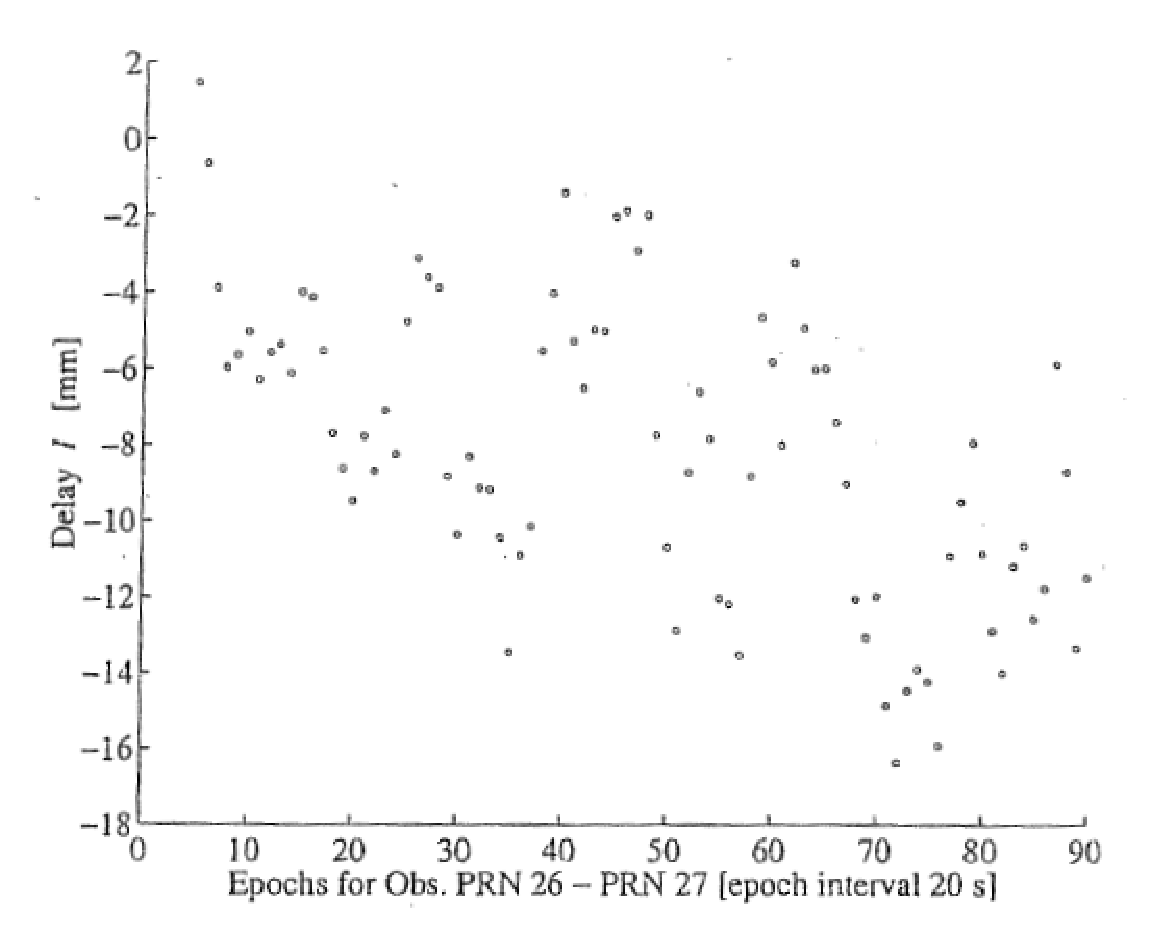
\includegraphics[width=0.4\linewidth]{TeX_files/Part03/chapter10/image/9-7}
	\caption{按照公式(10.21)对于相位双差,电离层延迟变化为2mm到-16mm,基线长度为4.6km}
	\label{fig:9-7}
\end{figure}

电离层延迟变化如图10.7,变化值很分散,在几个厘米以内。因此通过实验可以确定在I=0(没有延迟)的情况下是否能够被接受。

利用(10.20)的两个方程可以消掉电离层延迟项I,得到
\begin{equation}
	60\Phi_{1}/\lambda_{1}-77\Phi_{2}/\lambda_{2}=60N_{1}-77N_{2}
\end{equation}

因为$\frac{f_{1}}{f_{2}}=\frac{154}{120}=\frac{77}{60}$,所以出现系数60和70。但同时如此大的系数扩大了噪声。

\uppercase\expandafter{\romannumeral2}、另外一种消除电离层延迟I的方法是使用双频观测值。电离层延迟从几米到十几米变化不等。幸运的是电离层延迟是分散的,它取决于频率f。利用方程(10.8)我们可以获得双频电离层改正。首先利用同一颗卫星搭载在L1和L2载波上的两个伪距观测值:
$$
P_{1}=\rho^{*}+I-e_{1}
$$
$$
P_{2}=\rho^{*}+\alpha I-e_{2}
$$\\
忽略误差项 $e_{i}$,消掉I可得到理想伪距$\rho^{*}$:
$$
\rho^{*}=P_{1}-\frac{P_{1}-P_{2}}{1-\alpha}=P_{1}+1.545727802(P_{1}-P_{2})
$$\\
这个伪距的线性组合被称为消电离层组合。

\uppercase\expandafter{\romannumeral3}、接下来描述曾在第8章中使用过的一种简单的滤波方法$k_dd4$。它有4个未知量:理想伪距$\rho^{*}$,电离层延迟I和整周模糊度$N_{1}$、$N_{2}$。我们观测双频码伪距P和码相位$\Phi$。重写(10.9)如下:
$$
\begin{bmatrix}
1&1&0&0\\
1&-1&\lambda_{1}&0\\
1&\alpha&0&0\\
1&-\alpha&0&\lambda_{2}
\end{bmatrix}
\begin{bmatrix}
\rho^{*}\\I\\N_{1}\\N_{2}
\end{bmatrix}
=
\begin{bmatrix}
P_{1}\\\Phi_{1}\\P_{2}\\\Phi_{2}
\end{bmatrix}
-e
$$\\
独立观测值$P_{1}$,$\Phi_{1}$,$P_{2}$和$\Phi_{2}$的方差为$0.3^{2}$,$0.005^{2}$,$0.3^{2}$和$0.005^{2}m^{2}$。给出的$x_{0}$初始值,利用5个历元解含有4个未知量的4个方程。由于接收机的冷启动,早期的数据含有相当大的噪声。对于误差$\epsilon$的状态方程中$\rho^{*}$ ,I和模糊度的方差为100, 10, 0和0$m^{2}$,则输出结果包含 $\rho^{*}$,I,$N_{1}$和宽巷模糊度$N_{w}=N_{1}-N^{2}$的滤波值。

电离层延迟的绝对值变化非常剧烈,它取决于季节、纬度、这一天的时间以及其他参数。关于电离层的更多研究在Klobuchar 模型中(1996)进行了阐述。

\subsection{10.5.2 电离层延迟}

在纬度为$\varphi$的地区接收到的GPS信号的电离层延迟模型如下,其中天顶距离为 z = $90^{\circ}$-h。大气压力$P_{0}$ 的单位为豪巴,高度H的单位为千米,温度$T_{0}$的单位为开尔文,水汽分压$e_{0}$的单位为豪巴,则
\begin{equation}
	T=0.002277\frac{1+0.0026cos2\varphi+0.00028H}{cosz}(P_{0}+(\frac{1255}{T_{0}}+0.05)e_{0}).
\end{equation}\\

这个简单的模型可以以不同的方式被扩展。我们的目的是确定短基线向量并达到厘米级精度,而M-file 对流层计算程序能轻易满足这个要求,计算的天顶对流层延迟T$\approx$2.4 m。从公式可以看出对流层延迟与cosz成反比,因此在处理GPS观测数据时,截止高度角通常选为$15^{\circ}$。

M-file 对流层计算程序需要以下参数作为输入:

- sinel  卫星仰角的正弦,

- hsta  以千米为单位的测站高,高度hp以豪巴为单位的大气压力p,

- tkel  高度为htkel以开尔文为单位的表面温度,

- hum  高度为hhum以百分比为单位的湿度,

- hp  以千米为单位的进行压力测量的高度,

- htkel  以千米为单位的进行温度测量的高度和

- hhum  以千米为单位的进行湿度测量的高度。

这个对流层计算代码可能是最近出版的代码中对流层延迟计算结果最精密的。

天顶对流层延迟具有2\%的不确定性甚至更小。当天顶距小于$75^{\circ}$时,这个不确定性并不会增加很多。如果所有的伪距观测值含有的是一个常数偏差,那么计算的位置将不会受到影响,而仅仅是扩大了接收机钟差的偏差。但是如果对流层延迟不是常数,这将会影响定位点的高度。然而,对于短基线双差定位对流层延迟并不是很大的误差。

\subsection{10.5.3 码观测值上的多路径}

多路径效应是指卫星信号沿着多个路径到达接收机天线的情况。卫星发射的信号大部分直接达到接收机,但是部分信号受到周围表面的反射后才到达接收机。多路径效应取决于卫星的几何分布和接收机天线所处的环境,因此很难通过模型确定。24小时的长时间观测在一定程度上可以减小多路径效应的影响,而对于短时间观测,多路径效应是一个不可忽视的问题。

更多关于如何计算多路径效应的细节可参见\textbf{291(根据排版找到相应页码)}页。
		\section[模糊度的GOAD解法]{模糊度的GOAD方法\\The GOAD Method for Ambiguities}

		\section[模糊度的LAMBDA解法]{模糊度的LAMBDA解法\\The LAMBDA Method for Ambiguities}

		\section[GPS和时间]{GPS和时间\\GPS and Time}

		\section[动态实时定位]{动态实时定位\\Real-Time Kinematic Positioning}
	%%----------------------------第十章结束-------------------------%%
	
%-----------------------第三部分结束---------------------------%	

%-----------------------第四部分开始---------------------------%	
\part[大地测量和地球坐标]{大地测量和地球坐标\\Geodesy and Earth Coordinates}
% \第四篇[目录标题]{正文标题}
	%%----------------------------第十一章开始-------------------------%%
	\chapter[椭球面大地测量]{椭球面大地测量\\Geometry of the Ellipsoid}
	\minitoc %小标题
	\newpage%新页
		\section[旋转椭球]{旋转椭球\\The Ellipsoid of Revolution}

		\section[主曲率]{主曲率\\Principal Curvatures}

		\section[子午圈的长度]{子午圈的长度\\Length of a Meridional Arc}

		\section[法截面和测地线]{法截面和测地线\\Normal Section and the Geodesic}

		\section[曲线和测地线的Frenet公式]{曲线和测地线的Frenet公式\\Frenet`s Formulas on Curves and Geodesics}

		\section[克莱劳方程]{克莱劳方程\\Clairaut`s Equation}

		\section[测地线的性能]{测地线的性能\\The Behavior of the Geodesic}

		\section[直接和间接的大地测量]{直接和间接的大地测量\\The direct and reverse problems of geodesy}

		\section[算法]{算法\\Algorithms}
		
	%%----------------------------第十一章结束-------------------------%%
	
	%%----------------------------第十二章开始-------------------------%%
	\chapter[椭球面的正形投影]{椭球面的正形投影\\Differences of One-Way Observations}
	\minitoc %小标题
	\newpage%新页
		\section[直角坐标系到椭球坐标系]{直角坐标系到椭球坐标系\\Rectangular to Ellipsoidal Coordinates}

		\section[椭球的高斯投影]{椭球的高斯投影\\The Gaussian Mapping of the Ellipsoid onto the Plane}

		\section[递归最小二乘(与卡尔曼滤波)]{递归最小二乘(与卡尔曼滤波)\\Recursive Least Squares(and Kalman Filter)}
例4.4 \quad 假设我们已经计算了99个数$b_1,...,b_{99}$的平均数$\hat{x}_{99}$,出现一个新的数$b_{100}$,我们如何在不把前99个数再重新加一遍的情况下得到一个新的平均值$\hat{x}_{100}$(加上$b_{100}$)?我们只想利用$\hat{x}_{99}$和$b_100$。

这是新旧正确的组合$\hat{x}_{100}$,表现为两种形式:

新平均值 
\begin{equation}
\hat{x}_{100}=\frac{99}{100}\hat{x}_{99}+\frac{1}{100}b_{100}=\hat{x}_{99}+\frac{1}{100}(b_{100}-\hat{x}_{99})
\end{equation}
公式中第一项$\frac{99}{100}\hat{x}_{99}$是$(\frac{99}{100})$乘以$(\frac{1}{99})$再乘以$(b_1+b_2+...+b_{99})$,约去99,就是$(\frac{1}{100})$乘以这99个数的和(没有重新加一次!),加上额外的$(\frac{1}{100})$给出所有b的和,再除以100,这就是正确的平均值。

我们更喜欢第二张形式的递推公式(4.24)。通过复杂的创新$b_{100}-\hat{x}_{99}$得到右边更新的$\hat{x}_{99}$,这个创新表明了有多少“新信息”在$b_{100}$中。当$b_{100}$等于旧平均数,创新为0,在这种情况下,更新的$\hat{x}_{100}$就是原来的$\hat{x}_{99}$,校正=预测。

创新是将这个更新公式(4.24)乘以$\frac{1}{100}$,这个增益系数使这个公式正确。想到同样的方法$Ax=b$,从最小二乘解决方程$A_{old}x=b_{old}$入手,新的信息加入,新的观测值$b_{new}$,组合方程$Ax=b$通过最小二乘解出,组合系统为:
\begin{equation}
\begin{bmatrix}
A_{old} \\ A_{new}
\end{bmatrix}
\begin{bmatrix}
x
\end{bmatrix}
\begin{bmatrix}
b_{old} \\ b_{new}
\end{bmatrix}
\end{equation}
引导$\hat{x}_{new}$。

估值$\hat{x}_{new}$从整个系统$Ax=b$得到,在$b_{old}$中的数据仍然有助于$\hat{x}_{new}$,但是我们不想做相同的计算两次。

问题4.1  \quad 我们能否仅用$A_{new}$和$b_{new}$更新$\hat{x}_{old}$和$\hat{x}_{new}$?采取$C=I$
答案 \quad  既然$A^T=\begin{bmatrix} A^T_{old} & A^T_{new}\end{bmatrix}$,我们需要$A^TA$在正常方程:
\begin{equation}
A^TA=A^T_{old}A_{old}+A^T_{new}A_{new}=(known)+(new)
\end{equation}
然后在右边我们需要$A^Tb$,也涉及到新旧值:
\begin{equation}
A^Tb=A^T_{old}b_{old}+A^T_{new}b_{new}=A^T_{old}A_{old}\hat{x}_{old}+A^T_{new}b_{new}
\end{equation}

用$A^TA-A^T_{new}A_{new}$代替$A^T_{old}A_{old}$,然后乘以$(A^TA)^{-1}$找到$\hat{x}_{new}$:
\begin{equation*}
\hat{x}_{new}=(A^TA)^{-1}((A^TA-A^T_{new}A_{new})\hat{x}_{old}+A^T_{new}b_{new})
\end{equation*}

这个更新的公式简化了从原来的值产生新的$\hat{x}$,递推:
\begin{equation}
\hat{x}_{new}=\hat{x}_{old}+(A^TA)^{-1}A^T_{new}(b_{new}-A_{new}\hat{x}_{old})
\end{equation}
最后一项$b_{new}-A_{new}\hat{x}_{old}$是更新,这是我们对于观测值$b_{new}$的预测误差。如果误差为零,数据$b_{new}$与旧估计是完全一致的,没有理由去改变,因此$\hat{x}_{new}=\hat{x}_{old}$。

通常更新项$b_{new}-A_{new}\hat{x}_{old}$不为零,然后(4.28)乘上增益矩阵$K=(A^TA)^{-1}A^T_{new}$找到$\hat{x}$中的变化,增益矩阵是“放大器”,由K(卡尔曼)提出。注意到$A^TA$和$\hat{x}$在更新(4.26)和(4.28)有大小n,比m小。

例4.5 \quad (例4.4完整版)平均值$\hat{u}_{99}=\frac{1}{99}(b_1+...+b_99)$是一元99个方程的最小二乘解,99由1矩阵$A_{old}$是所有的:
\begin{equation*}
\begin{bmatrix}
1 \\ \dots \\ 1
\end{bmatrix}
u=
\begin{bmatrix}
b_1 \\ \dots \\ b_{99}
\end{bmatrix}
A^T_{old}A_{old}\hat{x}_{old}=A^T_{old}b_{old}
\end{equation*}
为:
\begin{equation*}
99\hat{x}_{old}=b_1+...+b_{99}
\end{equation*}
第100个方程是$u=b_{100}=b_{new}$,新的一行是$A_{new}=[1]$,检查所有:

(4.26)更新$A^TA$:
\begin{equation*}
A^TA=99(old)+1(new)=100
\end{equation*}

(4.28)更新$\hat{x}$:
\begin{equation*}
\hat{x}_{100}=\hat{x}_{99}+\frac{1}{100}(b_{new}-A_{new}\hat{x}_{old})=\hat{x}_{99}+\frac{1}{100}(\hat{x}_{100}-\hat{x}_{99})
\end{equation*}

更新的公式与方程(4.24)匹配,增益K是$(A^TA)^{-1}A_{new}=\frac{1}{100}$。

重要的是,你可能认为$A^TA=100$仅仅是对$\hat{x}_{100}$有用的一步,一点也不是,在最小二乘中,$A^TA$(及其逆)是比答案本身更有意义!当我们包含加权矩阵$C=\Sigma^{-1}$时,更新方程(4.26)给出$A^TCA$。我们已经知道为什么想要这个矩阵:逆矩阵$A^TCA=A^T\Sigma^{-1}A$量测$\hat{x}$的可信度P。

在这100个方程的例子中,$b_i$具有相等的可信度,它们有相同的方差$\sigma^2$,来自“标准”正态分布,它们都有$\sigma^2=1$,加权矩阵是$C=I$(正如我们所选),然后$A^TCA=100$的逆量测它们平均值$\hat{x}_{100}$的可信度,如果100个样本有相同的$\sigma^2$,它们的平均值有方差$\sigma^2/100$,当递推最小二乘更新$\hat{x}$时更新矩阵$P=(A^T\Sigma^{-1}A)^{-1}$。

	\subsection[卡尔曼滤波实例]{卡尔曼滤波实例\\Kalman Filter by Example}
	卡尔曼滤波应用在时变最小二乘中,状态x是不断变化的。在离散时间中,我们在每一个$t=i$时间下产生一个估计$\hat{x}_i$,早期的测量仍然给出关于目前状态的信息,因为这种状态是相关的,所以那些$b's$被包含在计算$\hat{x}_i$中。它们可能作用小一些,但是仍然起作用。
	
	例4.6 \quad  有一个未知数x,你的心率,医生第一次测量为$b_1$,之后测量为$b_2$,如果没有理由预测改变,最好的估计$\hat{x}$将是平均数$\frac{1}{2}(b_1+b_2)$,但是如果预测脉率随着年龄的增加而变慢,一个“状态方程”将在这个时间间隔内表示预期变化$c_1$,状态方程为:
	\begin{equation}
	x_2-x_1=c_1+error\epsilon_1
	\end{equation}
	现在我们看关于两个状态值$x_1$和$x_2$。三个方程,它们通过(4.29)联系,观测值和状态方程为:
	\begin{equation}
	x_1 \quad =b_1 
	\end{equation}
	\begin{equation*}
    -x_1+x_2=c_2 
	\end{equation*}
	\begin{equation*}		
	\quad x_2 = b_2
	\end{equation*}
	为:
	\begin{equation*}
	\begin{bmatrix}
	A_{old} \\ A_{state} \\ A_{new}
	\end{bmatrix}
	\begin{bmatrix}
	x_{old}  \\ x_{new}
	\end{bmatrix}
	=
	\begin{bmatrix}
	b_{old} \\ c_{state} \\ b_{new}
	\end{bmatrix}
	\end{equation*}
	重要的是,在这三个方程中都有误差,状态方程并不精确,因为我们的心脏并非以同样的方式变慢,在(4.29)中的状态误差$\epsilon_1$有它自己的方差$\upsilon^2_1$。我们假设误差$e_1,\epsilon_1,e_2$是独立的,这使得一个递归计算(卡尔曼滤波)成为可能。
	
	状态$x_i$通常是一个向量,具有像位置和速度这样的成分(思考追踪一颗空间卫星,或者移动车辆中的GPS),然后(4.29)从旧$x_i$中预测新的位置$x_{i+1}$。通常在$b_i$中会有测量误差的协方差矩阵$\Sigma_i$,在$x_{i+1}=F_ix_i+c_i$中有状态方程误差的协方差$V_i$。		
  
   \begin{figure}
		\centering
		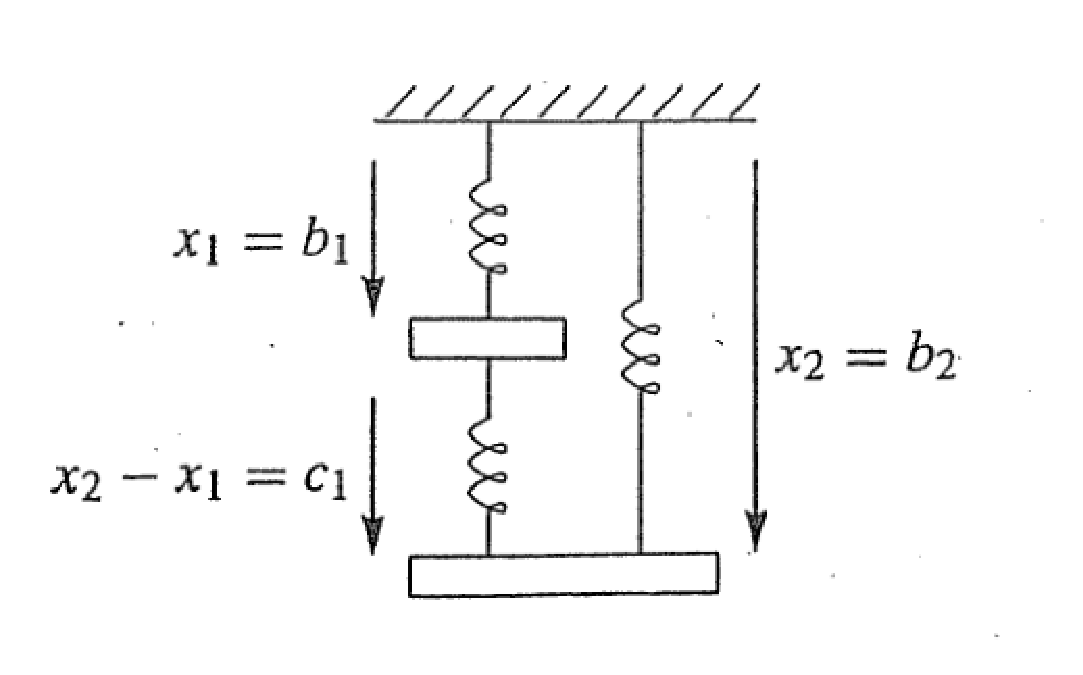
\includegraphics[width=0.7\linewidth]{TeX_files/Part02/chapter04/image/4-4}
		\caption{观测方程和状态方程的质量弹簧当量}
		\label{fig:4-4}
	\end{figure}	
	卡尔曼在每个预测/校正中增加一个弹簧 
	\begin{equation*}
	\hat{x}_{1|1}=b_1  \qquad  \hat{x}_{2|1}=b_1+c_1
	\end{equation*}
	\begin{equation*}
	\hat{x}_2=\hat{x}_{2|2}=\frac{1}{3}(b_1+2b_2+c_1)
	\end{equation*}
	
	解法 \quad  (4.30)中加权最小二乘原则仍给出$\hat{x}_1$和$\hat{x}_2$,最小化为:
	\begin{equation}
	E=\frac{1}{\sigma^2_1}(b_1-x_1)^2+\frac{1}{v^2_1}(c_1+x_1-x_2)^2+\frac{1}{\sigma^2_2}(b_2-x_2)^2
	\end{equation}
	
	加权正常方程$A^TCA=A^TCb$将有$C^{-1}=diag(\sigma^2_1,v^2_1,\sigma^2_2)$,有$C=I,\sigma_1=\sigma_2=V_1=1$:
	\begin{equation}
	\begin{bmatrix}
	\hat{x}_1  \\ \hat{x}_2
	\end{bmatrix}
	=
	\begin{bmatrix}
	b_1-c_1  \\  b_2+c_1
	\end{bmatrix}
	\end{equation}
	给出:
	\begin{equation*}
	\hat{x}_1=\frac{1}{3}(2b_1+b_2-c_1)
	\end{equation*}
	\begin{equation*}
	\hat{x}_2=\frac{1}{3}(b_1+2b_2+c_1)
	\end{equation*}
	
	最新的估计$\hat{x}_2$给了最新的观测值$b_2$一个较大的权重$\frac{2}{3}$。
	
	现在递归计算。关键的一点是$A^TCA$是三对角矩阵(在第8章中,当状态x是一个向量时,它将成为块对角矩阵)。观测方程$A_ix_i=b_i$与状态方程$x_{i+1}=F_ix_i+c_i$相连接,在三对角矩阵$A^TCA$中前向消去法总是一个递归乘法器和一个支点,然后回代是第二个递归,落后于时间。
	
	关键是事实本身,前向递归在观测方程、多达状态方程、还包括时间t=i的基础上,找到最佳估计$\hat{x}_{i|i}$,通常情况下,最终状态的估计$\hat{x}_{n|n}$是我们想要的,然后忘记回代这一步。
	
	回代这一步是调整先前的$\hat{x}_{i|i}$去解释之后的观测方程和状态方程,在时间i之后,以这种方式返回被称为“平滑”,它会使正常方程$A^TCA\hat{x}=A^TCb$产生正确的答案$\hat{x}_{i|n}$。
	
	甚至说寻找$\hat{x}_{i|i}$的前向递归是一个两步法。先前的一步$\hat{x}_{i-1|i-1}$通过时间$i-1$使用所有的信息,接下来状态方程给出一个预测,然后观测值$b_i$加上一个校正,与卡尔曼的滤波一起产生$\hat{x}_{i|i}$,预测和校正为:
	\begin{equation*}
	\hat{x}_{i|i-1}=F_{i-1}\hat{x}_{i-1|i-1}+c_i
	\end{equation*}
	\begin{equation*}
	\hat{x}_{i|i}=\hat{x}_{i|i-1}+K_i(b_i-A_i\hat{x}_{i|i-1})
	\end{equation*}
	该校正像使用增益矩阵$K_i$更新一样被写入,新数据是$c_i$和$b_i$,我们通过最小二乘,一次增加一个方程求解这个完整的系统$Ax=b$。
	
	在递归最小二乘中,有更多的一些东西需要我们计算——估计$\hat{x}_{i|i}$的可信度。协方差矩阵$P_{i|i}=(A^TCA)^{-1}_i$也是递归更新,卡尔曼滤波的每一步都增加一行(或块)到A和C中,一列(或块)到$A^T$和$C$中。预测校正步骤计算$P_{i|i-1}$和$P_{i|i}$,在$\hat{x}_{i|i-1}$和$\hat{x}_{i|i}$中的误差协方差。
	
	公平地说,卡尔曼滤波变得复杂,即使这个计划一直向前。所有的作者试图找到一个清晰的方法去推导$\hat{x}_{i|i}$和$P_{i|i}$的矩阵公式(有多种方式给数值以不同的递归)。平方根滤波用$LDL^T$或$QR$来减少当方差变得很小或很大时的数值不稳定性,我们对卡尔曼滤波的阐述将在第八章进行。
	
	最重要的一点是,协方差矩阵$P_{i|i}$像状态$x_i$具有相同的大小,这个大小与在第i步的观测数量$m_i$无关,如果我们更新最佳拟合直线,我们的矩阵保持2乘以2。
	
	例4.7 \quad (心率)在C=I(单位方差)下,递归找出P和$\hat{x}$:
	
	从$x_1=b_1$开始:\quad\quad  $A_{1|1}=[1]$  给出 $P_{1|1}=(A^TA)^{-1}_{1|1}=[I]$

	加上$x_2-x_1=c_1$:\quad $A_{2|1}=\begin{bmatrix} 1 & 0 \\ -1 & 1 \end{bmatrix}$
	和 $(A^TA)^{-1}_{2|1}=\begin{bmatrix} 1 & 1 \\ 1 & 2 \end{bmatrix}$ 给出  $P_{2|1}=2$
	
	包括$x_2=b_2$:\quad  $A_{2|2}=\begin{bmatrix} -1 & 0 \\ -1 & 1 \\ 0 & 1 \end{bmatrix}$
	和 $(A^TA)^{-1}_{2|2}=\frac{1}{3}\begin{bmatrix} 2 & 1 \\ 1 & 2 \end{bmatrix}$ 给出  $P_{2|2}=\frac{2}{3}$。
	
	第一次估计是$\hat{x}_{1|1}=b_1$(没有平滑!),使用状态方程进行接下来预测$\hat{x}_{2|1}=b_1+c_2$,使用最后的$A_{2|2}$得到校正$\frac{1}{3}(b_1+2b_2+c_1)$。
	
	那些方差$P_{2|1}=2$和$P_{2|2}=\frac{2}{3}$是$(A^TA)^{-1}_{2|1}$和$(A^TA)^{-1}_{2|2}$的最后一项,向量$x_i$引导块的支点$P^{-1}$。这里的2和$\frac{2}{3}$也被看作$b_1+c_1$和$\frac{1}{3}(b_1+2b_2+c_1)$的系数平方和。
	
	回代(平滑)在(4.32)中,调整$\hat{x}_{1|1}=b_1$成为$\hat{x}_1=\frac{1}{3}(2b_1+b_2-c_1)$。
		\section[正态分布与$\chi^{2}$]{正态分布与$\chi^{2}$\\The Normal Distribution and $\chi^{2}$}

		\section[地图叠加]{地图叠加\\Multiplication of the Mapping}

		\section[平滑]{平滑\\Smoothing}

		\section[最好的等角投影]{最好的等角投影\\Best Possible Conformal Mapping}
	
	%%----------------------------第十二章结束-------------------------%%

\backmatter
% bibliography, glossary and index would go here.

\end{document}